\documentclass[nobib, b5paper]{tufte-book}

\hypersetup{colorlinks}% uncomment this line if you prefer colored hyperlinks (e.g., for onscreen viewing)

%%
% Book metadata
\title{Optimization of Future Mobile Communication Systems using Deep Learning}
\date{01/04/2020}
\author[Jakob Thrane]{Jakob Thrane}
\publisher{DTU Fotonik}

\usepackage[backend=biber, natbib=true, style=numeric]{biblatex}
\addbibresource{references.bib}
\usepackage{tikz}
\usepackage{caption}
%\usepackage{subcaption}
\usepackage{booktabs}
\usepackage{graphicx}
\usepackage{fancyvrb}
\usepackage{xspace}
\usepackage[caption=false, font=footnotesize]{subfig}
\usepackage{glossaries}
\glsdisablehyper
\usepackage{amsmath,amssymb,amsfonts}
\usepackage{algorithmic}
\usepackage{bm}
\usepackage{xcolor}
\usepackage{xargs}
\usepackage{color}
\usepackage{listings}
\usepackage{pdfpages}
\usepackage{epigraph}
\usepackage{titlesec}
\makeatletter
\titleformat{\part}[display]
  {\Huge\scshape\filright}
  {\partname~\thepart:}
  {20pt}
  {\thispagestyle{epigraph}}
\makeatother
\setlength\epigraphwidth{.6\textwidth}


\newacronym{ssp}{SSP}{Small-scale Parameter}
\newacronym{lsp}{LSP}{Large-scale Parameter}
\newacronym{los}{LOS}{Line-Of-Sight}
\newacronym{snr}{SNR}{Signal-to-Noise Ratio}
\newacronym{sinr}{SINR}{Signal-to-Interference-Plus-Noise Ratio}

\newacronym{rma}{RMa}{Rurual Macro}
\newacronym{uma}{UMa}{Urban Macro}
\newacronym{umi}{UMi}{Urban Micro}
\newacronym{inh}{InH}{Indoor Hotspot}
\newacronym{embb}{eMBB}{Enhanced Mobile Broadband}
\newacronym{mmtc}{mMTC}{Massive machine type communications}
\newacronym{urllc}{URLLC}{Ultra-reliable and low latency communications}
\newacronym{nlos}{NLOS}{Non-Line-Of-Sight}
\newacronym{tdd}{TDD}{Time Division Duplex}
\newacronym{fdd}{FDD}{Frequency Divison Duplex}
\newacronym{mimo}{MIMO}{Multiple-Input and Multiple-Output}
\newacronym{srs}{SRS}{Sound Reference Signal}
\newacronym{csi}{CSI}{Channel State Information}
\newacronym{mmwave}{mmWave}{Milimeter Wave}
\newacronym{ofdm}{OFDM}{Orthogonal frequency-division multiplexing}
\newacronym{dde}{DDE}{decision-directed estimation}
\newacronym{pe}{PE}{Pilot-based Estimation}
\newacronym{o2i}{O$2$I}{Outdoor-To-Indoor}
\newacronym{i2i}{I$2$I}{Indoor-To-Indoor}
\newacronym{o2o}{O$2$O}{Outdoor-To-Outdoor}
\newacronym{nbiot}{NB-IoT}{Narrowband Internet of Things}
\newacronym{lte}{LTE}{Long-Term Evolution}
\newacronym{nr}{NR}{$5$G New Radio}
\newacronym{3gpp}{$3$GPP}{3rd Generation Partnership Project}
\newacronym{itu}{ITU}{International Telecommunication Union}
\newacronym{cdl}{CDL}{Cluster Delay Line}
\newacronym{tdl}{TDL}{Tapped Delay Line}
\newacronym{h-udn}{H-UDN}{Heterogeneous UltraDense Network}
\newacronym{mdt}{MDT}{Minimization of Drive Tests}
\newacronym{monster}{MONSTeR}{MObile Networks SimulaToR}
\newacronym{otdoa}{OTDOA}{Observed Time Difference of Arrival}
\newacronym{ue}{UE}{User Equipment}
\newacronym{ut}{UT}{User Terminal}
\newacronym{son}{SON}{Self-Organizing Network}
\newacronym{siso}{SISO}{Single Input Single Output}
\newacronym{enb}{eNB}{Evolved Node B}
\newacronym{gnb}{gNB}{Next Generation Node B}
\newacronym{ici}{ICI}{Inter-Cell Interference}
\newacronym{fir}{FIR}{Finite Impulse Reponse}
\newacronym{pci}{PCI}{Primary Cell Identifier}
\newacronym{qpsk}{QPSK}{Quadrature Phase-Shift Keying}
\newacronym{ul}{UL}{Uplink}

\newacronym{kpi}{KPI}{Key Performance Indicator}

\newacronym{dnn}{DNN}{Deep Neural Network}
\newacronym{nn}{NN}{Neural Network}
\newacronym{relu}{ReLU}{Rectified Linear Unit}
\newacronym{cnn}{CNN}{Convolutional Neural Network}
\newacronym{dl}{DL}{Deep Learning}
\newacronym{ml}{ML}{Machine Learning}
\newacronym{rmse}{RMSE}{Root-Mean-Square Error}
\newacronym{mse}{MSE}{Mean-Squared Error}
\newacronym{mae}{MAE}{Mean Absolute Error}
\newacronym{dqn}{DQN}{Deep Q-network}
\newacronym{mc}{MC}{Monte Carlo}
\newacronym{lms}{LMS}{Least-Mean-Square}
\newacronym{ols}{OLS}{Ordinary least squares}
\newacronym{ai}{AI}{Artificial Intelligence}
\newacronym{rsrp}{RSRP}{Reference Signals Received Power}
\newacronym{rsrq}{RSRQ}{Reference Signal Received Quality}
\newacronym{rssi}{RSSI}{Received Signal Strength Indicator}
\newacronym{iq}{IQ}{In-phase and Quadrature components}
\newacronym{mmse}{MMSE}{Minimum mean square error}

\newacronym{r_and_s}{R\&S}{Rohde \& Schwarz}
\newacronym{gnss}{GNSS}{Global Navigation Satellite System}
\newacronym{dtm}{DTM}{Digital Terrain Model}
\newacronym{gpu}{GPU}{Graphics Processing Unit}
\newacronym{lidar}{LIDAR}{Light Detection and Ranging}
\newacronym{mno}{MNO}{Mobile Network Operator}
\newacronym{roi}{ROI}{Region of Interest}
\newacronym{osm}{OSM}{OpenStreetMap}
\newacronym{dsm}{DSM}{Digital Surface Model}
\newacronym{sdn}{SDN}{Software-Defined Network}


\newacronym{gui}{GUI}{Graphical User Interface}
\newacronym{api}{API}{Application Programming Interface}
\newacronym{gis}{GIS}{Geographical Information System}
\newacronym{lpwan}{LPWAN}{Low Power Wide Area Network}
\newacronym{ls}{LS}{Least-Squares}
\newacronym{se}{SE}{Spectral Efficiency}
\newacronym{dci}{DCI}{Downlink Control Information}



\newcommand{\uma}[1]{\gls{uma}\_#1}

%%
% If they're installed, use Bergamo and Chantilly from www.fontsite.com.
% They're clones of Bembo and Gill Sans, respectively.
%\IfFileExists{bergamo.sty}{\usepackage[osf]{bergamo}}{}% Bembo
%\IfFileExists{chantill.sty}{\usepackage{chantill}}{}% Gill Sans

%\usepackage{microtype}

%%
% colors
\definecolor{deepblue}{rgb}{0,0,0.5}
\definecolor{deepred}{rgb}{0.6,0,0}
\definecolor{deepgreen}{rgb}{0,0.5,0}


%%
% For graphics / images
\setkeys{Gin}{width=\linewidth,totalheight=\textheight,keepaspectratio}
\graphicspath{{graphics/}}


% The fancyvrb package lets us customize the formatting of verbatim
% environments.  We use a slightly smaller font.
\fvset{fontsize=\normalsize}


%%
% Prints argument within hanging parentheses (i.e., parentheses that take
% up no horizontal space).  Useful in tabular environments.
\newcommand{\hangp}[1]{\makebox[0pt][r]{(}#1\makebox[0pt][l]{)}}

%%
% Prints an asterisk that takes up no horizontal space.
% Useful in tabular environments.
\newcommand{\hangstar}{\makebox[0pt][l]{*}}


%%
% Some shortcuts for Tufte's book titles.  The lowercase commands will
% produce the initials of the book title in italics.  The all-caps commands
% will print out the full title of the book in italics.
\newcommand{\vdqi}{\textit{VDQI}\xspace}
\newcommand{\ei}{\textit{EI}\xspace}
\newcommand{\ve}{\textit{VE}\xspace}
\newcommand{\be}{\textit{BE}\xspace}
\newcommand{\VDQI}{\textit{The Visual Display of Quantitative Information}\xspace}
\newcommand{\EI}{\textit{Envisioning Information}\xspace}
\newcommand{\VE}{\textit{Visual Explanations}\xspace}
\newcommand{\BE}{\textit{Beautiful Evidence}\xspace}

\newcommand{\TL}{Tufte-\LaTeX\xspace}

% Prints the month name (e.g., January) and the year (e.g., 2008)
\newcommand{\monthyear}{%
  \ifcase\month\or January\or February\or March\or April\or May\or June\or
  July\or August\or September\or October\or November\or
  December\fi\space\number\year
}


% Prints an epigraph and speaker in sans serif, all-caps type.
\newcommand{\openepigraph}[2]{%
  %\sffamily\fontsize{14}{16}\selectfont
  \begin{fullwidth}
  \sffamily\large
  \begin{doublespace}
  \noindent\allcaps{#1}\\% epigraph
  \noindent\allcaps{#2}% author
  \end{doublespace}
  \end{fullwidth}
}

% Inserts a blank page
\newcommand{\blankpage}{\newpage\hbox{}\thispagestyle{empty}\newpage}

\usepackage{units}

% Typesets the font size, leading, and measure in the form of 10/12x26 pc.
\newcommand{\measure}[3]{#1/#2$\times$\unit[#3]{pc}}

% Macros for typesetting the documentation
\newcommand{\hlred}[1]{\textcolor{Maroon}{#1}}% prints in red
\newcommand{\hangleft}[1]{\makebox[0pt][r]{#1}}
\newcommand{\hairsp}{\hspace{1pt}}% hair space
\newcommand{\hquad}{\hskip0.5em\relax}% half quad space
\newcommand{\TODO}{\textcolor{red}{\bf TODO!}\xspace}
\newcommand{\na}{\quad--}% used in tables for N/A cells
\providecommand{\XeLaTeX}{X\lower.5ex\hbox{\kern-0.15em\reflectbox{E}}\kern-0.1em\LaTeX}
\newcommand{\tXeLaTeX}{\XeLaTeX\index{XeLaTeX@\protect\XeLaTeX}}
% \index{\texttt{\textbackslash xyz}@\hangleft{\texttt{\textbackslash}}\texttt{xyz}}
\newcommand{\tuftebs}{\symbol{'134}}% a backslash in tt type in OT1/T1
\newcommand{\doccmdnoindex}[2][]{\texttt{\tuftebs#2}}% command name -- adds backslash automatically (and doesn't add cmd to the index)
\newcommand{\doccmddef}[2][]{%
  \hlred{\texttt{\tuftebs#2}}\label{cmd:#2}%
  \ifthenelse{\isempty{#1}}%
    {% add the command to the index
      \index{#2 command@\protect\hangleft{\texttt{\tuftebs}}\texttt{#2}}% command name
    }%
    {% add the command and package to the index
      \index{#2 command@\protect\hangleft{\texttt{\tuftebs}}\texttt{#2} (\texttt{#1} package)}% command name
      \index{#1 package@\texttt{#1} package}\index{packages!#1@\texttt{#1}}% package name
    }%
}% command name -- adds backslash automatically
\newcommand{\doccmd}[2][]{%
  \texttt{\tuftebs#2}%
  \ifthenelse{\isempty{#1}}%
    {% add the command to the index
      \index{#2 command@\protect\hangleft{\texttt{\tuftebs}}\texttt{#2}}% command name
    }%
    {% add the command and package to the index
      \index{#2 command@\protect\hangleft{\texttt{\tuftebs}}\texttt{#2} (\texttt{#1} package)}% command name
      \index{#1 package@\texttt{#1} package}\index{packages!#1@\texttt{#1}}% package name
    }%
}% command name -- adds backslash automatically
\newcommand{\docopt}[1]{\ensuremath{\langle}\textrm{\textit{#1}}\ensuremath{\rangle}}% optional command argument
\newcommand{\docarg}[1]{\textrm{\textit{#1}}}% (required) command argument
\newenvironment{docspec}{\begin{quotation}\ttfamily\parskip0pt\parindent0pt\ignorespaces}{\end{quotation}}% command specification environment
\newcommand{\docenv}[1]{\texttt{#1}\index{#1 environment@\texttt{#1} environment}\index{environments!#1@\texttt{#1}}}% environment name
\newcommand{\docenvdef}[1]{\hlred{\texttt{#1}}\label{env:#1}\index{#1 environment@\texttt{#1} environment}\index{environments!#1@\texttt{#1}}}% environment name
\newcommand{\docpkg}[1]{\texttt{#1}\index{#1 package@\texttt{#1} package}\index{packages!#1@\texttt{#1}}}% package name
\newcommand{\doccls}[1]{\texttt{#1}}% document class name
\newcommand{\docclsopt}[1]{\texttt{#1}\index{#1 class option@\texttt{#1} class option}\index{class options!#1@\texttt{#1}}}% document class option name
\newcommand{\docclsoptdef}[1]{\hlred{\texttt{#1}}\label{clsopt:#1}\index{#1 class option@\texttt{#1} class option}\index{class options!#1@\texttt{#1}}}% document class option name defined
\newcommand{\docmsg}[2]{\bigskip\begin{fullwidth}\noindent\ttfamily#1\end{fullwidth}\medskip\par\noindent#2}
\newcommand{\docfilehook}[2]{\texttt{#1}\index{file hooks!#2}\index{#1@\texttt{#1}}}
\newcommand{\doccounter}[1]{\texttt{#1}\index{#1 counter@\texttt{#1} counter}}


\titlecontents{part}%
    [0pt]% distance from left margin
    {\addvspace{0.25\baselineskip}}% above (global formatting of entry)
    {}% before w/ label (label = ``Part I'')
    {Part~\uppercase\thecontentslabel}% before w/o label
    {\hfill\thecontentspage}% filler and page (leaders and page num)
    [\vspace*{0.5\baselineskip}]% after

\titlecontents{chapter}%
    [4em]% distance from left margin
    {}% above (global formatting of entry)
    {\contentslabel{2em}\textit}% before w/ label (label = ``Chapter 1'')
    {\hspace{3em}\textit}% before w/o label
    {\hfill\thecontentspage}% filler and page (leaders and page num)
    [\vspace*{0.5\baselineskip}]% after

\titlecontents{section}%
    [4.5em]% distance from left margin
    {}% above (global formatting of entry)
    {\contentslabel{2em}\textit}% before w/ label (label = ``Chapter 1'')
    {\hspace{3em}\textit}% before w/o label
    {\hfill\thecontentspage}% filler and page (leaders and page num)
    [\vspace*{0.5\baselineskip}]% after
%%%% End additional code by Kevin Godby
\titlecontents{subsection}%
    [7em]% distance from left margin
    {}% above (global formatting of entry)
    {\contentslabel{4em}\textit}% before w/ label (label = ``Chapter 1'')
    {\hspace{2em}\textit}% before w/o label
    {\qquad\thecontentspage}% filler and page (leaders and page num)
    [\vspace*{0.5\baselineskip}]% after
%%%% End additional code by Kevin Godby

\titleformat{\chapter}%
  {\huge\rmfamily\itshape\color{black}}% format applied to label+text
  {\llap{\colorbox{black}{\parbox{3cm}{\hfill\itshape\Huge\color{white}\thechapter}}}}% label
  {8pt}% horizontal separation between label and title body
  {}% before the title body
  []% after the title body

\setcounter{secnumdepth}{3}
\setcounter{tocdepth}{1}
\makeglossaries
\makeindex


\begin{document}

% Front matter
\frontmatter

% r.1 blank page
%\blankpage

% r.3 full title page
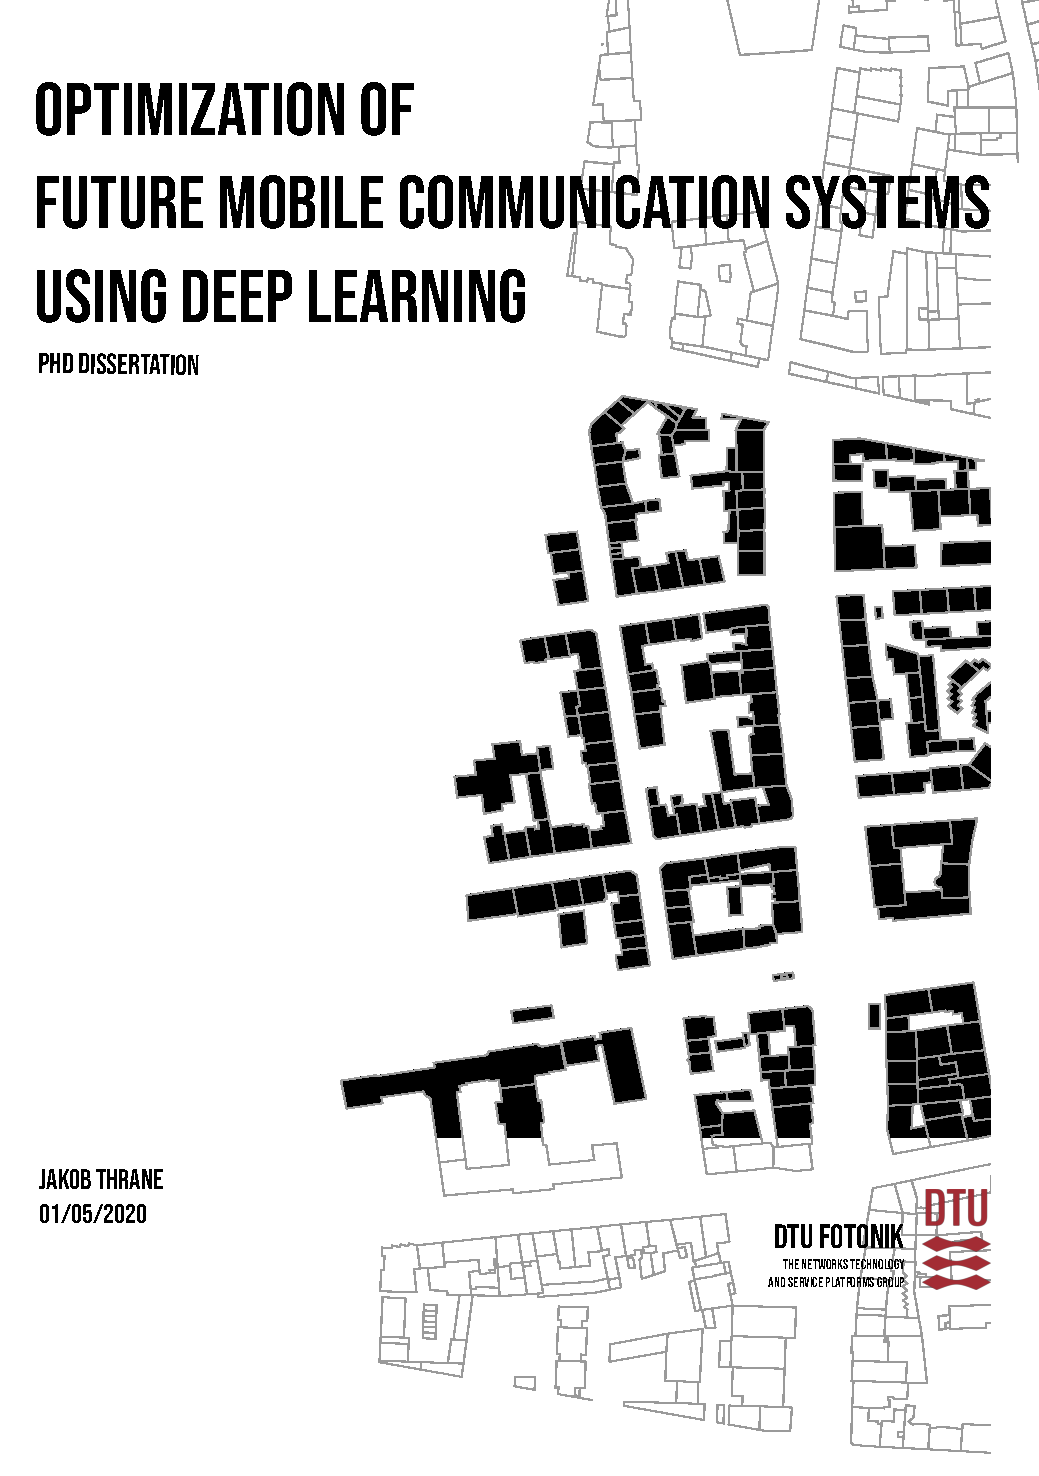
\includepdf[pages=-]{chapters/thesis_frontpage.pdf}


% v.4 copyright page
\newpage
\begin{fullwidth}
~\vfill
\thispagestyle{empty}
\setlength{\parindent}{0pt}
\setlength{\parskip}{\baselineskip}
Copyright \copyright\ \the\year\ \thanklessauthor

\par\smallcaps{Published by \thanklesspublisher}

\par\smallcaps{tufte-latex.github.io/tufte-latex/}

\par Licensed under the Apache License, Version 2.0 (the ``License''); you may not
use this file except in compliance with the License. You may obtain a copy
of the License at \url{http://www.apache.org/licenses/LICENSE-2.0}. Unless
required by applicable law or agreed to in writing, software distributed
under the License is distributed on an \smallcaps{``AS IS'' BASIS, WITHOUT
WARRANTIES OR CONDITIONS OF ANY KIND}, either express or implied. See the
License for the specific language governing permissions and limitations
under the License.\index{license}

\par\textit{First printing, \monthyear}
\end{fullwidth}

\chapter*{Resumé}
Mobil kommunikationsnetværk er komplekse systemer der består af utrolige ingeniørmæssige præstationer. De nuværende og fremtidige mobil kommunikationssystemer er, og i fremtiden endnu mere, komplekse at styre og optimere. Sub-optimale mobilenetværk resulterer i ineffektive implementeringer der forårsager dårlig kundeoplevelse og øgede drifts- og kapitaludgifter for netværksoperatører. Deep Learning har i de seneste år leveret imponerende resultater i komplekse opgaver så som talegenkendelse og billedegenkendelse. Kompleksiteten af mobile kommunikationssytemer forventer at stige og Deep Learning er blevet anerkendt som en nødvendig løsning til at overvinde sådanne udfordringer. Indholdet i denne afhandling er udforskning af nye metodikker fra Deep Learning værktøjskassen. Denne afhandling har bidraget med adskillige anvendelser af Deep Learning for at løse komplekse problemer i mobile kommunikationssystemer. Specifikt præsenteres der tre nye metoder.

1) Nøjagtige forudsigelser af signalkvalitet på umålte lokalisationer med lav datakompleksitet ved hjælp af geografiske billeder. 2) Væsentlige forbedringer af kanalestimering af opnået på sparsomme og få reference signaler i uplink transmission og 3) En adaptiv reinforcement indlæringsalgorithme der er i stand til at undgå interferens i radiomiljøet. Udover dette præsenteres flere empiriske undersøgelser, mest bemærkelsesværdigt kan disse resultater opsummeres som følgende. 1) Komplekse ray-tracing metoder viser ingen præsentations forbedring sammenlignet med enkle empiriske modeller til udbredelsesmodellering af radiobølger i mobile kommunikationssystemer. 2) Nuværende modeller til dybe indendørs scenarier, f.eks. tuneller viser dårlig ydevne og kræver nye løsninger.

Resultaterne præsenteret i afhandlingen viser at Deep Learning kan opnå betydelig præsetations forbedringer på det fysiske lag af mobile kommunikationssystmer. Effektive implementeringer af Deep Learning metoder og beregningskompleksisteten heraf er fundet essentielle for fremtidig forskning. Dette er således også en nødvendighed for at reducere det tidskrævende aspekt af at finde passende modelkompleksitet. Endeligt, indlejring af såkaldt \emph{expert knowledge} er en nødvendighed for anvendelsen af Deep Learning i mobile kommunikationssystemer for at sikre pålideligheden.
\chapter*{Abstract}
Mobile Communication networks are complex systems consisting of many incredible engineering achievements. The current and future mobile communication systems are, and in the future even more so, complex to manage and optimize. Sub-optimal mobile networks result in cost-ineffective deployments causing poor customer experience and increased operational and capital expenses for operators. \acrfull{dl} have in the recent years provided with impressive results in complex tasks such as speech recognition and computer vision. The complex reality of mobile communication systems is expected to increase, and \gls{dl} has been hailed as a necessary component co overcome such challenges. The content of this dissertation is the exploration of novel methodologies available in \acrshort{dl} toolbox. This dissertation has resulted in several advancements for applying \gls{dl} to complex tasks in mobile communication systems. Accurately, three novel methods are presented. 

1) Accurate signal quality predictions in unseen locations with low data complexity using geographical images. 2) Significant improvements to channel estimation applied on sparse reference signals in uplink and 3) An adaptive reinforcement learning algorithm capable of avoiding contamination in the radio environment. In addition to this, several study items are presented. Most noticeably the outcome can be summarized as, 1) Complex ray-tracing methods show little to no performance gain compared to simple empirical models for mobile communication propagation modelling. 2) Current deep-indoor propagation models show poor generalized performance and require novel solutions.

The results presented throughout the dissertation are conclusive and show significant performance gains offered by \gls{dl}-based solutions on the physical layer of mobile communication systems. The implementation and thus, the computational complexity of the proposed \gls{dl} methods are found to be essential and essential for future research. Thus, efficient implementations are necessary to reduce the time-consuming aspect of tuning model complexity which enable further discovery of the fundamental capabilities of the given method. Finally, embedding \emph{expert knowledge} into \gls{dl}-based solutions is seen as a necessity for the application in mobile communication systems to ensure reliability and transparency.
\chapter*{Preface}

This dissertation is submitted in partial fulfillment of the requirments for a Doctoral Degree


\section*{Acknowledgements}




\printglossary[type=\acronymtype, nonumberlist, title=Acronyms]

% r.5 contents
\tableofcontents


%\listoffigures
%\listoftables

% r.7 dedication
\cleardoublepage
~\vfill
\begin{doublespace}
\noindent\fontsize{18}{22}\selectfont\itshape
\nohyphenation
Dedicated to those who appreciate \LaTeX{} 
and the work of \mbox{Edward R.~Tufte} 
and \mbox{Donald E.~Knuth}.
\end{doublespace}
\vfill
\vfill


% r.9 introduction
\cleardoublepage
\chapter*{Introduction}\label{ch:introduction}
\addcontentsline{toc}{section}{\nameref{ch:introduction}}
Mobile communication systems have over the past two decades, become a foundation for modern society. Communication has always been a fundamental necessity for human society, but the recent years have indeed shown how great of an engineering achievement cellular networks are. The mobile phone has evolved into a device that enables an enormous amount of services. For most people, what goes on behind the scenes of a mobile phone is considered black magic. Most people do not question it as long as it just \emph{works}. However, when it does not work, or \emph{no service} is displayed, the annoyance is more significant than anything. Regardless of the annoyance level reached, these mobile communication services are paramount to modern society, if not only for entertainment but also for essential emergency communication services. As technology evolves, so does mobile communication systems. The development and on-going process of deploying \gls{nr} solutions is the foundation for a multitude of communication services. The capabilities of \gls{nr} are many, one of which is the expected industrial revolution where automatization is in focus. However, first and foremost, to offer increased capacity and coverage. The increased capacity, lower latency and improved energy efficiency are vital properties of \gls{nr}-based networks. These improved capabilities are driven not only by demand but also by necessity. 

\gls{ai} have in recent years been shown to be capable of solving complex problems surpassing human performance in tasks such as image recognition or language translation. These performances have not gone unnoticed and have attracted incredible attention from mainstream media. The models behind these advances are in broad strokes identified by \acrfull{ml}. While modern mobile communication systems may be an incredible feat of engineering, it is still faced with many complex problems of management and optimization. The recent advances in \gls{ml} offering automated feature engineering through \acrlong{dl} models coupled with the increased demand for mobile communication systems, sparked the PhD project behind this dissertation. Current mobile communication systems are advanced, sophisticated, and any additions must be selected with patience and deliberation. The adaptability of \acrlong{dl} has been hailed as an essential part in overcoming these problems and a key enabler for future mobile networks. This dissertation seeks to explore the role and feasibility of \gls{ai} solutions in current and future mobile communication systems through novel applications. 

The main limitation of mobile communication networks is the transmission of information over the air using radio waves. The radio environment in mobile communication systems is difficult to characterize due to many complex interactions on both a macroscopic and microscopic level. The fundamental theoretical understanding of radio propagation has been established and can offer insight into this complex and dynamic environment; however, at the cost of extreme computational complexity. To ensure reliable transmission in the current mobile systems, it requires an enormous amount of so-called channel state information. This information is to ensure the right actions are taken when transmitting to and from a user. This amount of information is significant. So significant that it in practice is capable of storing $2^{24}$ channel coefficients per millisecond per operating base station \cite{Studer2018}. The base station is the entity that connects to mobile devices present in the environment. Data quantity is the main driver for \acrlong{dl}-solutions.  By formalizing problems as learning objectives, \acrlong{dl} can be used to obtain correlation, information and insight from otherwise insensible data. The data quantities of the radio environment, coupled with the requirements for \acrlong{dl} defines the areas of contributions within this dissertation.


\section*{Areas of contribution}
The focus of the contributions within this dissertation is on the so-called \emph{physical layer} of mobile communication systems, seen in Fig. \ref{fig:areas_of_contribution}. For any communication system, this layer is associated with the practicalities of transmitting and receiving the raw information over the transmission medium. In the case of mobile communication systems, the transmission medium is foremost considered \emph{the air}. 


\begin{figure*}
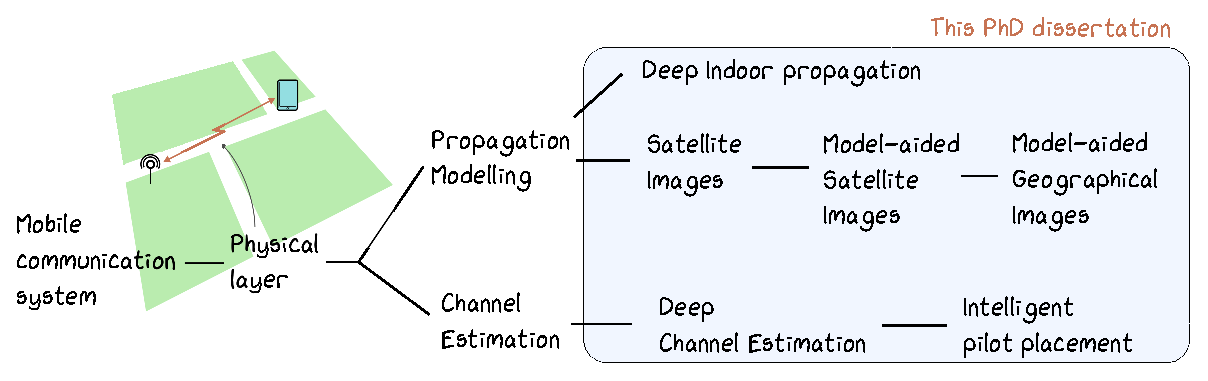
\includegraphics[width=\textwidth]{chapters/figures/intro_figure.eps}
\caption{Contributions of this dissertation}\label{fig:areas_of_contribution}
\end{figure*}

\section*{Contributions}

The contributions of this dissertation can be reduced to the following specific items. 

\begin{itemize}
    \item Chapter \ref{ch:channelmodellingbasics}, A provided Ray-tracing model for mobile communication systems offer no performance improvements compared to existing empirical models.
    \item Chapter \ref{ch:satelliteImages}, Deep Learning can significantly improve path loss estimation for unseen locations.
    \item Chapter \ref{ch:satelliteImages}, Geographical Images contain information useful for path loss prediction that can be extracted with supervised learning.
    \item Chapter \ref{ch:deepindoor}, Deep-indoor propagation characteristic is shown to be determined by a complex combination of geo-statistical features.
    \item Chapter \ref{ch:deepindoor}, Deep Learning is identified as an essential tool for engineering features used for modelling deep-indoor propagation.
    \item Chapter \ref{ch:channel_estimation}, Channel estimation in uplink transmission can significantly be improved by using Deep Learning.
    \item Chapter \ref{ch:channel_q_learning}, Deep Reinforcement Learning can enable autonomous solutions for designing optimum pilot placement in uplink.
\end{itemize}

\noindent Specifically, the above have been formalized into peer-review published research papers. The list of associated research papers can be found below.


\section*{Paper contributions}

The asterisk \emph{*} denotes research papers awaiting peer-review. They can be found in Appendix \ref{app:submitted_papers}.

\vspace{2em}

\noindent \textbf{Thrane, J.} \&  Artuso, M. \&  Zibar, D. \&  Christiansen, H. L. (2018). \textit{Drive Test Minimization Using Deep Learning with Bayesian Approximation}. 2018 IEEE 88th Vehicular Technology Conference (VTC-Fall) \cite{Thrane2018DriveApproximation}

\vspace{2em}


\noindent Artuso, M. \&  \textbf{Thrane, J.} \&  Christiansen, H. L. (2018). \textit{User-Centric Power Saving in Self-Organizing Mobile Networks.} 2018 IEEE 88th Vehicular Technology Conference (VTC-Fall) \cite{Artuso2018User-CentricNetworks}

\vspace{2em}

\noindent \textbf{Thrane, J.} \&  Zibar, D. \&  Christiansen, H. L. (2019). \textit{Comparison of Empirical and Ray-Tracing Models for Mobile Communication Systems at 2.6 GHz}. 2019 IEEE 90th Vehicular Technology Conference (VTC2019-Fall) \cite{Thrane2019ComparisonGHz}

\vspace{2em}

\noindent \textbf{Thrane, J.} \&  M., Zibar, D. \&  Christiansen, H. L. \textit{Model-aided Deep Learning Method for Path Loss Prediction in Mobile Communication Systems at 2.6 GHz}. IEEE Access 2020 \cite{Thrane020ModelAidedDeepLearning}

\vspace{2em}

\noindent \textbf{Thrane, J.} \&  Christiansen, H. L. \textit{Pilot Placement Method for Future Cellular Systems in Uplink at 2 GHz using Deep Q-Learning}. IEEE OJVT 2020, submitted \cite{Thrane2020PilotQ-Learning} *


\vspace{2em}

\noindent \textbf{Thrane, J.} \&  Sliwa, B. \& Wietfeld, C. \& Christiansen, H. L. \textit{Deep Learning-based Signal Strength Prediction Using Geographical Images and Expert Knowledge}. IEEE Globecom 2020, submitted \cite{Thrane2020DeepKnowledge} *

\vspace{2em}
\noindent 
Ruepp S. \& Mateo A. C.  \& Malarski K. M.  \& \textbf{Thrane J.}  \&  Petersen, M. N. (2018). \textit{Internet of Things Connectivity in Deep-Indoor Environments}. 2018 9th International Conference on the Network of the Future \cite{Malarski2018DemonstrationCases}

\vspace{2em}
\noindent Malarski, K. M. \& \textbf{Thrane, J.} \&  Bech, M. G. \&  Macheta, K. \&  Christiansen, H. L.  \& Petersen  M. N. \& Ruepp  S. \textit{Investigation of deep indoor NB-IoT propagation attenuation}. IEEE 90th Vehicular Technology Conference 2019 Fall (VTC2019-Fall) \cite{Malarski2019InvestigationAttenuation}

\vspace{2em}
\noindent \textbf{Thrane, J.} \&  Malarski, K. M. \& Christiansen, H. L. \& Ruepp, S. \textit{Experimental Evaluation of Empirical NB-IoT Propagation Modelling in a Deep-Indoor Scenario}. IEEE Globecom 2020, submitted \cite{Thrane2020ExperimentalScenario} *


\section*{Dataset contributions}

\noindent \textbf{Thrane, J.} \& Christiansen, H. L. \textit{Mobile Communication System Measurements and Satellite Images}. IEEE DataPort 2019 \cite{1xf4-eg98-19}

\vspace{2em}
\noindent \textbf{Thrane, J.} \& Christiansen, H.L. \& Bech, M. G. \textit{Technical University of Denmark LTE drive test measurements} IEEE DataPort 2020 \cite{keyt-8g44-20}

\section*{Implementation contributions}

\noindent \textbf{Thrane, J.} \textit{GitHub repository for the dissertation: Optimization of Mobile Communication Systems using Deep Learning}. GitHub 2020 \cite{Thrane2020RepositoryLearning}.


\section*{Dissertation structure}
 
The dissertation is structured into three separate parts. 

\paragraph{Part I} In chapter \ref{ch:monster} an introduction to the state of mobile communication systems and optimizations hereof is given along. Along with this, a motivation for \gls{dl}-based solutions is given. Additionally, in chapter \ref{ch:mlbasics} a brief introduction to \gls{ml} and \gls{dl} is provided along with short descriptions of the most important \gls{dl} terms used for the remainder of the dissertation. 

\paragraph{Part II} In chapter \ref{ch:channelmodellingbasics} introduces traditional means of modelling the wireless channel. This includes a focus on an empirical and ray-tracing model. A comparison study of the traditional models are presented, discussed and concluded. Chapter \ref{ch:satelliteImages} contains a novel methodology for estimating signal quality metrics for unseen locations in mobile communication systems utilizing geographical images. The method is evaluated and improved over several iterations; the finding of each iteration is presented. Chapter \ref{ch:deepindoor} contains the study of wireless transmission in a deep-indoor situation, utilizing \gls{nbiot} terminology. The results of a comprehensive measurement campaign are presented along with an identified direction for \gls{dl}-based solutions.  The findings of applying \gls{dl} for radio propagation modelling is summarized and discussed in chapter \ref{ch:dl_radio_summary}.

\paragraph{Part III} In chapter \ref{ch:pilot_sequence} so-called pilot signals for current cellular systems are introduced. The current and future issues of so-called \emph{pilot contamination} is introduced along with a discussion of existing solutions found in the literature. In chapter \ref{ch:channel_estimation} a novel method for channel estimation is presented. The results and challenges of the method are discussed in detail. In chapter \ref{ch:channel_q_learning}, a reinforcement learning method for combating pilot contamination and improving channel estimation is presented. Finally, the challenges associated with \gls{dl}-based solutions for channel estimation and pilot optimization are discussed. 

\paragraph{Part IV} In chapter \ref{ch:contributions} an overview of the contributions offered by this dissertation is given. The contributions are discussed in detail, and a perspective to practical considerations is given. Additionally, the challenges identified throughout the dissertation are summarized. A discussion of \gls{dl}-based solutions in mobile communication systems is given. Finally, in chapter \ref{ch:conclusion} a conclusion is provided.







%%
% Start the main matter (normal chapters)
\mainmatter

\epigraphhead[350]{}
\part{Data is a requirement}
\chapter{Optimization of Mobile Communication Systems}\label{ch:monster}

Mobile Communication systems (or Cellular Networks) have become an essential part of modern society. For the better parts of 2 decades, the systems we use in our daily lives have evolved continuously, mostly behind the scenes, but also directly observable for everyone. The introduction of smartphones have required a revolution to existing mobile communication systems and have brought us technologies such as \gls{lte} $4$G and the to-be-deployed in the nearest future \acrfull{nr}. The content of these systems is probably one of the greatest engineering feats achieved in modern times. Such systems are increasingly complex, and future systems will most definitely introduce more complexity in order to increase capacity for the end-users efficiently. Behind this complexity resides the wireless transmission over the air that is the backbone of the systems. By understanding the fundamental physical properties of wireless transmission, the systems and sub-systems of existing technologies have been designed to very effectively transmit and receive signals over long distances. Understanding the wireless channel satisfactory has been a long-standing engineering achievement and has been improved immensely for these modern systems compared to just a few decades ago. The key to further improvement of these systems is by understanding every little detail that makes up the complex and mysterious act that is wireless transmission. So far, the working and operational systems that are deployed and used throughout the world is a manifest to the fundamental understanding of wireless transmission. 

As with any communication system, it is relevant to recall the well-known Shannon–Hartley theorem \cite{Tse2005FundamentalsCommunication}.

\begin{equation}\label{eq:shannon}
    C = B \log_2 \left( 1 + \frac{S}{N} \right)
\end{equation}

The theorem describes the information rate, also known as capacity $C$, is determined by 1) The so-called bandwidth $B$, 2) the received signal power $S$ and 3) the noise of the communication channel $N$. The Shannon-Hartley theorem determines the fundamental limits of capacity and has so far not been proven wrong. If the conditions of the communication channel are static and constant, the only way to increase capacity is by 1) increasing bandwidth and 2) increasing the signal received power.

Increasing bandwidth can be done by introducing new carrier frequencies, as is the case with \gls{lte} and \gls{nr}. A multitude of frequencies is deployed in the current cellular systems to increase the necessary capacity required for users \cite{Goldsmith2005WirelessCommunications, Molisch2007}. For this, we look towards the current and future of cellular networks in terms of so-called \gls{h-udn}.


% \begin{itemize}
%     \item Introduce the concept of cellular networks in broad strokes 
%     \item Mention capacity is dependent on two things, bandwidth, receiver signal power and the noise level
%     \item Introduce provisioning of systems and the relation to capacity
%       \item introduce the concepts of heterogeneous cellular networks
%     \item More capacity is always desired but comes at an expensive cost of deployment
%     \item optimisation of deployment is paramount to ensure reliable capacity and connectivity 
% \end{itemize}

\section{Heterogeneous Cellular Networks}
\gls{h-udn} also termed just Heterogeneous Cellular Networks, is a modification for improving the capacity of existing systems. Classical cellular networks consist primarily of centralised base stations effectively providing both coverage and capacity solutions to all users localised in the site. By doing so, the bandwidth and thus capacity is essentially limited by the base station. Both \gls{lte} and \gls{nr} seek to densify the cellular network architecture to improve bandwidth, and the channel conditions effectively increasing the available capacity. The densification in \gls{h-udn} consists specifically of introducing additional relays, and base station with reduced antenna arrays into the existing site. These are termed micro, pico and femtocells, depending on the deployment and overall requirements \cite{Yunas2015, Ge2016}. The result of this is effectively a reduction in the inter-site distance between the terminals and the deployed base stations. Such a case is depicted in Fig. \ref{fig:hudn_drawing}. The modification is furthermore to accommodate a large amount of available bandwidth in \gls{mmwave} frequencies. The use of \gls{mmwave} is expected to be an essential part of \gls{nr} solutions enabling massive capacity boosts. However, \gls{mmwave} suffer over longer distances to increased path loss and reduced penetration properties. By reducing the inter-site distance in future \gls{h-udn}, novel solutions such as \gls{mmwave} is feasible. 

\begin{figure*}
    \centering
    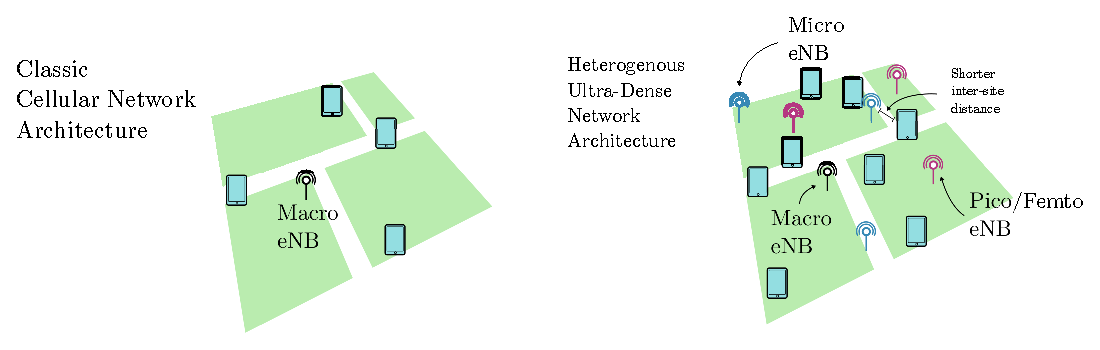
\includegraphics{chapters/part_pathloss/figures/hudn_drawing.eps}
    \caption{Additional sites with different transmissions frequencies are added to the existing network architecture to boost capacity.}
    \label{fig:hudn_drawing}
\end{figure*}


A classic cellular architecture usually consists of a single Macro base station that is tasked with supplying both coverage and capacity. In \gls{h-udn} such centralised base stations are expected only to handle control signals and wide-area low capacity coverage. The smaller base stations are thus tasked with the majority of user data management and the overall capacity. The necessary evolution and deployment of such systems are inevitably subject to complex deployment and management situations. The authors outline this in \cite{Taufique2017} that discuss the challenges and opportunities associated with the planning of such complex systems. The authors discuss the severe need for accurate models for the many aspects of such systems, including energy management, interference modelling, and wireless channel models amongst many others. 




\section{Optimization of Mobile systems}


Two phases describe the life-cycle of mobile communication systems. Before deployment (the planning phase) or during operation (optimization phase) \cite{Taufique2017}. In literature, it is found that the term \emph{optimization phase} is used to describe when the network has been deployed and is operational. However, in this dissertation, the term \emph{optimization} is used to define the improvement of a specific situation or resource. For instance, the planning phase can be optimised to ensure that the future addition of small cells and other unplanned deployments can be achieved without fundamental challenges related to the deployed network. Classic planning techniques are primarily focused on the optimisation of the number of base stations and their location. This has later evolved into a multitude of parameters to be considered. For instance, transmission specific parameters such as antenna tilt, transmission power and others can be used in the planning process to optimise the coverage and capacity of the system. With the emerging technologies of $4$G and $5$G, the planning phase have been extended with an extensive list of parameters  \cite{Taufique2017}. For instance, new capacity improving solutions such as \gls{mimo} require constant configuration and optimisation to ensure the maximum efficiency of the systems is utilised. The evolving complexity of these systems require \glspl{mno} to approach cellular planning differently. This have pushed so-called \gls{son} features to be an essential part of deployment and operation of future mobile communication systems. Additionally, and considered beyond the scope of this dissertation, is network virtualisation and \gls{sdn} methodologies  \cite{Taufique2017}.


In short and brief terms, \gls{son} is the automatization and self-configuration of processes related to the planning and operation of mobile networks. The features of \gls{son} is to ensure that mobile networks are cost-efficient as additional solutions for improving capacity make their way into existing systems. This can be achieved at many levels, for instance, by having a standardised and almost autonomous procedure for cellular deployment that optimise all associated parameters. An overview of \gls{son} features can be found in \cite{Jorguseski2014Self-organizingTrends} and references herein.

\acrlong{son} require intelligent methodologies for effectively providing with the much-needed intelligence. Learning methodologies, as provided by \acrfull{ml} is encompassed to fulfil these requirements. A comprehensive study of \gls{ml} applied for \gls{son} can be found in \cite{Klaine2017ANetworks}. 

In any case, \gls{son} features or not, the optimisation of mobile communication systems is effectively also a result of obtaining the necessary data representative of the deployment, or in the case of the planning phase to-be deployment. This can either be done through measurements, which is limited to deployed networks, or simulations. Simulations have over the recent years sparked an increasing amount of research papers and is a core technique for the optimisation of cellular networks and research hereof. Regardless, radio measurements is a key and necessary element for the performance evaluation of cellular networks and even more so with increased network complexity. Obtaining such measurements can be done with regular and frequent \emph{drive tests}. However, as the complexity of these systems increases the drive testing in itself becomes increasingly expensive. 

\subsection{Drive testing}\label{sec:drive_testing}

\begin{figure}
    \centering
    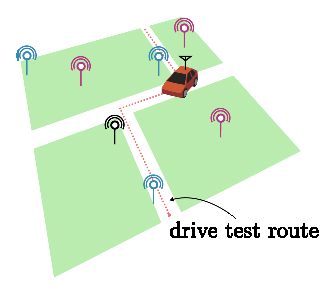
\includegraphics[width=.5\textwidth]{chapters/figures/drive_test_illustration.eps}
    \caption{Drive testing is an effective way of obtaining radio measurements, but time exhaustive}
    \label{fig:my_label}
\end{figure}


Drive testing consists simply of attaching an antenna on top of a vehicle and driving around areas of deployment. Examples of such data sets can be found in Appendix \ref{app:drive_test_study_2017} and \ref{app_drive_test_study_2020}. Obtaining drive test measurements is a costly affair as deployment regions can cover large or hard-to-reach areas. Optimising the drive test procedure have been attempted by utilising hardware in the loop and 3D acceleration \cite{Charitos2017} with promising results. However, the default solution is to practically fit a car with the right equipment and drive around. Drivable roads effectively limit the granularity. Measurement solutions exist for doing it on foot and are useful in non-drivable areas and indoor coverage situations \cite{ROMESmanual}. 

\subsection{\glspl{kpi}}
Depending on the mobile communication system, the \gls{kpi} differ. For \gls{lte} and \gls{nr} an extensive list of relevant metrics exist. For this dissertation the focus in on the following reference signal based metrics
\begin{itemize}
    \item \gls{rsrp}
    \item \gls{rssi}
    \item \gls{rsrq}
\end{itemize}

A set of so-called reference signals are used to infer the value of the above metrics. Additionally to these, \gls{sinr} is a commonly used metric and is a direct indication of the achievable information rate for a given transmission link. The freqeuncy resuse of modern mobile communications introduce interference between neighbouring sites. The metric of \gls{rsrp} is the measure of reference signal power for a single base station. The reference signals between neighbouring base stations differ and therefore an independent measurement of the received power can be obtained. This is different for \gls{rssi} which contains the average power of all reference signals observed. Therefor, \gls{rssi} is the measure of neighbouring base stations within reach of the receiver. \gls{rsrq} is fraction between the \gls{rsrp} and \gls{rssi} and is thus a metric of infering the interference caused by neighbouring base stations. A detailed description of these metrics can be found in \cite{Molisch2007}.

By inspecting the resulting drive tests, improvements to existing deployments can be made. For instance, if any coverage holes or interference sources are identified, they can be remedied to improve capacity and coverage and thus the resulting customer experience. Drive tests are a common practise utilised by \gls{mno} to evaluate the efficiency of deployments continually. Performing drive testing is an extremely costly affair, and there is a significant opportunity to cut both capital and operational costs by reducing the number of needed drive tests. Solutions related to reducing drive testing is termed \gls{mdt}


\subsection{Minimization of drive testing}
\gls{mdt} is introduced with Release 10 of \gls{lte} and introduces principles for minimising the required drive testing. The approach uses reports from the attached \glspl{ue} to evaluate not only the coverage but also the capacity of mobile communication systems. In essence, the concept consists of having the \gls{ue} transmit back a report detailing necessary and important \glspl{kpi} such as \gls{rsrq} and \gls{rsrp} among others. By combining these measured parameters with a localisation metric, so-called \emph{radiomaps} can be constructed. 

In the case of radiomaps, this can be used in combination with so-called \emph{kriging} methodologies enabling interpolation between the received \gls{kpi} reports. By doing so, useful approximations of capacity and coverage can be estimated given only a few measurements (sparse). By doing so, it enables the deduction and analysis of any existing coverage holes and other coverage impairments \cite{Bi2018EngineeringManagement}. 

However, such methods are dependent on accurate positioning. \gls{mdt} as per Release 10 \cite{3GPP2017} can utilize \gls{gnss} solutions if present in the \gls{ue}. However, doing so have to significant drawbacks \cite{Schloemann2016}. 

1) The accuracy of \gls{gnss} when not under open sky suffers from substantial inaccuracies. These inaccuracies are notably the case for indoor scenarios. 

2) The power draws from any \gls{gnss} solutions drain the battery of \glspl{ue} which is not ideal. 

Additionally, \glspl{ue} produce a noticeably difference in the \glspl{kpi} due to different quality electronics and antenna sub-systems \cite{Karstensen2017}. This further complicates the procedure of estimating coverage maps.

The localisation of users is paramount to minimising drive testing. Localisation is not only a necessary parameter for \gls{mdt} but also a necessity for emergency services to localise users in distress. One solution for doing so is utilising the so-called \gls{otdoa}. The parameter is useful for localising users in the radio environment \cite{Johansson2012} and can be used effectively for \gls{mdt} reports. However, utilising such a parameter can yield \emph{overly-optimistic expectations} when introducing a distinct increase in the number of neighbouring base stations \cite{Sivers2015, Schloemann2016}. 

While \gls{mdt} is an efficient way of obtaining measurements for current and future cellular systems, a traditional way of evaluating coverage and capacity include the use of so-called \emph{simulation environments}. 

\subsection{Simulation}
Mobile networks are costly to deploy; thus, network simulation is a powerful and necessary tool for the optimisation and development of future cellular networks. Simulators enable insights that may otherwise be infeasible to obtain through practical deployments. For instance, this includes the estimation of coverage and capacity for a given propagation scenario. It provides with essential insights into, for instance, the optimum locations of the required base stations. Or the upper and lower capacity bounds. By doing so, the properties of the systems can be evaluated and reevaluated to accommodate any needs related to, for instance, existing customers or economic considerations. Network simulators are essential for the future of wireless systems as also indicated by the authors in \cite{Cavalcanti2017}. 

Additionally, as this dissertation is focused around the application of \gls{dl} model, it is logical to use simulation tools for not only data generation but also studying existing optimisation procedures. During the development of the presented models and solutions throughout this dissertation, a significant number of various implementations were completed. It quickly realised that such implementations might be useful for the community. Consequently it was made open-source \cite{monster}$^1$.
\begin{marginfigure}
1 The tool found in \cite{monster} implements the majority of the empirical path loss models found in Chapter \ref{ch:channelmodellingbasics}. A majority of figures throughout this dissertation is created with the use of the framework. The framework is engineered to be modular and has significant ease of implementation for additional modules and extensions. A guide for contribution can be found in the repository. The foundation of the framework is built on the \texttt{LTE toolbox} by MathWorks. This includes also the specific implementations of the fast-fading models of \gls{tdl} and \gls{cdl} as briefly introduced in Chapter \ref{ch:channelmodellingbasics}.
\end{marginfigure}


\subsection{Channel models}

Radio propagation models or wireless channel models is an essential part of the design of mobile communications systems, and future systems even more so. The multitude of frequencies, bandwidths, and overall transmission complexity is subject to many different and complex interactions in the radio environment. Knowing how specific configurations of the communication system perform is essential to optimisation in both the planning and deployment phase of mobile networks. Models for emulating and simulating wireless channels have been an essential part of designing cellular systems as configurations, and new technologies can be tested cost-effectively. Statistics of wireless impairments can be deduced from obtained measurements (for instance, by using drive testing) and can be used in the planning and development of mobile communication solutions. The use of such statistics is a standard procedure and has resulted in the highly effective and straightforward \emph{empirical} wireless channel models. 

Channel models have been an essential element in the planning of mobile communication systems for a very long time \cite{Taufique2017, Cavalcanti2017}. By estimating and approximating the impact of the wireless channel changes and optimisation of the communication system can be achieved. For instance, channel models may enable the study of coverage for a given set of deployed cells. If the accuracy of the channel models are high, and coverage holes in the deployment can be identified, the deployment may be optimised to improve capacity and coverage. All this without doing expensive drive testing.

Modelling wireless interactions is a complex task, and for this reason, a multitude of channel models exist, with different model complexity. The study of the wireless channel has resulted in a few \emph{default} channel models—each with a different purpose. A brief introduction to such models can be found in Chapter \ref{ch:channelmodellingbasics}.

The introduction of \gls{h-udn} and \gls{mmwave} impose new stringent requirements for channel models and the applications for use in \gls{nr} mobile networks 
\cite{Wang2018}. Not only is a wide range of supported frequencies required, but also, more importantly, a wide range of propagation scenarios are needed to improve the performance of the models. 

The applications of channel models are expected not to be limited to the planning and deployment phases of future mobile communication systems. Recently, the talks of so-called anticipatory- and cognitive-networking is expected to be a primary driver for future technologies such as advanced \gls{son} techniques (for improving the optimisation capabilities of cellular systems) and autonomous vehicles \cite{Bui2017ATechniques, Zhang2018}. So, it can be found that accurate wireless channel models are essential to the optimisation of current systems but also a necessity for future systems. The trend of new and improved wireless channel models are furthermore essential to enable the development of solutions for future mobile communication systems. This results in the development of novel methods and solution to not necessarily require a full measurement campaign, which is time-consuming and expensive. Improved channel models thus effectively lead to improved solutions for future mobile communication systems. However, it is essential that improvements to current channel models also consider computational complexity, not only concerning the required data but also in terms of the resulting computational run-times.


\section{Is Deep Learning applicable to Mobile Communication systems?}
\gls{ml} has been hailed to be a key enabler in future mobile communication systems due to the capabilities of learning complex mapping functions. \gls{ml} is capable of learning complex functions through data observations that may otherwise be challenging to engineer. As discussed through the majority of this chapter, future mobile communication systems consist of many complex interactions and sub-systems. Therefore \gls{ml}-based solutions are regarded as an essential element in future cellular systems \cite{Li2017IntelligentIntelligence, Klaine2017ANetworks}. 
 
The specific capabilities of \gls{ml}-based solutions have been shown in recent literature. For instance, in \cite{OShea2017, Dorner2018, Aoudia2018} the authors show how a \gls{dl} model (a subfield of \gls{ml}) can be trained to learn the entire physical layer of a wireless communication system, in what they term \emph{end-to-end} learning. The adaptive model is capable of learning a full transmitter and receiver implementation yielded by the conditions of a channel model using a \gls{nn}. In other words, all sub-systems in a regular \gls{ofdm}-based receiver and transmitter can be learned by obtaining the right measurements. While this may not be feasible for practical systems, it shows the use case of \gls{dl} models in wireless communication system design.


A massive survey paper discussing the use cases of \gls{ml} in wireless network systems can be found in \cite{Zappone2019}. The authors discuss \emph{\gls{ai}-based Wireless Networks} that is driven entirely on data. The authors discuss the future of wireless networks and argue that these networks will consist of extreme complexity which means traditional approaches to network design and management are ineffective or as they print it: \emph{no longer adequate}. This particular point is the point that this chapter is trying to underline and define from the perspective of mobile communication systems. 


This dissertation will attempt to answer the question \emph{"Is Deep Learning applicable to Mobile Communication systems?"} through several novel \gls{dl} applications for mobile communication systems. The state of current mobile communication systems is massive and complex. Therefore, the provided answers will only be related to a reduced scope of applications. The physical layer is identified as a promising area for \gls{dl} applications, due to 1) the data quantities provided by radio measurements, and 2) the unknown characteristics (to some extend) of the radio propagation environment.  In chapter \ref{ch:mlbasics} a very brief introduction to the overwhelming world of \gls{ml} and \gls{dl} is given along with useful literature. 
\chapter{No innovation without data}\label{ch:mlbasics}

The area of \gls{ml} have evolved significantly over the past decade. This development and progression are partly due to the increased availability of computing resources and open-source libraries. Applying\gls{ml} in the year of 2020 is no longer limited to knowledgeable mathematicians/software engineers that are well-versed within the field. Drag-and-drop type interfaces for the non-programmer are even available through services such as Amazon Web Services making it access-able to everyone interested. \gls{ml} have been shown in recent years to improve specific tasks, and solve complex problems. For instance, massive performance gains have been achieved in computer vision and speech recognition tasks. For example, Google Translate is no longer many million lines of code. It is reduced to an adaptive model that has learned from many experiences \cite{Wu2016GooglesTranslation}. So not only has \gls{ml} reduced the complexity of solving the problem, but it has also improved the performance of such a system quite significantly. The most significant gains can, however, be seen in the area of computer vision. State-of-the-art \gls{ml} algorithms can surpass human performance in tasks such as image classification. Stories such as these, and many others, have caused \gls{ml} to find its way to mainstream media. \gls{ml} also termed \emph{\gls{ai}} is foreseen to be the solution to many complex problems where we as humans have great difficulties engineering solutions. However, such solutions come at the cost of transparency. Many \gls{ml} models provide solutions that even the engineers constructing them do not understand. This lack of transparency has increased with the recent introduction of \gls{dl}, a sub-field of \gls{ml} that learns from raw data. These models can have many millions of parameters, and the solution they offer can be challenging to interpret. 

The purpose of this chapter is to outline standard terms associated with the field of \gls{ml} as used throughout this dissertation.



\section{Machine Learning basics}

The tools of \gls{ml} is separated into different families of learning. These are known as \emph{supervised}-, \emph{unsupervised}-, and \emph{reinforcement} learning. Each of these families has different approaches to modelling and is summarised below. 

\paragraph{Supervised Learning}

Is considered the primary and most successful area of \gls{ml}. Supervised learning attempts to construct a mapping function between input $x$ and output $y$ through a function $f(\cdot)$. Thus the task of supervised learning is to find a function $f(\cdot)$ that can map between $x$ and $y$. To formulate a supervised learning problem, input data, as well as observations, are required. 

\paragraph{Unsupervised Learning}

Attempts to learn the underlying function of the data. Thus the task is to find a lower-dimensional latent variable such that the input can be represented by a function $f(\cdot)$ and a latent variable $z$. Subsequently, unsupervised learning is applied where no observations are available, but the data in itself contains information that may be challenging to represent \cite{M.Bishop2006}.

\paragraph{Reinforcement Learning}

Is the idea of learning through feedback. Reinforcement Learning systems are tasked with learning optimal policies. Policies can be defined as taking the \emph{correct} action given a specific state/observation of the system to optimize. Through interacting with the system/environment, the policies are optimized with respect to a reward metric. The metric is to reward or penalize the reinforcement learning system if a good or bad action is taken for a given observation. Over trial and error (i.e. iterations) such a reinforcement learning system learns the optimal policies and will provide the actions that maximize the reward. 

\subsection{Iterative learning}
The learning process in \gls{ml} methods differs significantly from tool to tool. The primary tools used throughout this dissertation are based on iterative algorithms, as commonly associated with such \gls{ml} models as \gls{nn}. It should be noted that not all \gls{ml} tools are based on iterative learning processes. \emph{Classic} \gls{ml} tools are based on analytical mathematics that uses all available observations for computing and learning. Such models as \gls{nn} use an iterative approach to learning from the data. This approach offers not only performance improvements for large datasets but also feasibility in terms of computational runtime. Iterative learning can be shown to be capable of converging towards optimal solutions in both convex and non-convex problems \cite{M.Bishop2006}. A simple example of adaptive iterative learning is attempted given below:

\emph{Adaptive filters} is a relatively intuitive example of iterative learning and can be found in most modern electronic devices. As to whether adaptive filters can be defined as \gls{ml} is up to the reader. However, many of the same principles associated with \gls{ml} are employed. 

The purpose of adaptive filters is to find a filter that approximates a dynamic and unknown system. In mobile communication, such an adaptive filter is available at the receiver in an attempt to \emph{equalize} the changes imposed by the wireless channel. Such a tool is also known generally as an \emph{equalizer} and can be found in most communication systems. The problem in wireless communication is the dynamic and unknown channel; we call it $H$. The channel imposes distortions and noise to the transmitted and originated waveform. With the presence of noise and distortions caused by the channel, the original signal must be extracted to enable and construct a communication system. For this, an adaptive filter is commonly used.  As shown in Fig. \ref{fig:adaptive_filter_system}, the purpose of the adaptive filter is to approximate the channel response $H$. An adaptive filter can be formalized as a \gls{fir} filter and takes the form 

\begin{equation}\label{eq:fir}
    y[n] = \sum_{i=0}^N w_n[i]x[n-i]
\end{equation}

Where $y[n]$ is the samples at the output of the system in time, $w_n$ are the filter weights with a finite number of weights, and $x_n$ are the samples at the input of the system. Thus, the objective is to find the coefficients/weights of $w_n$. 

\begin{marginfigure}
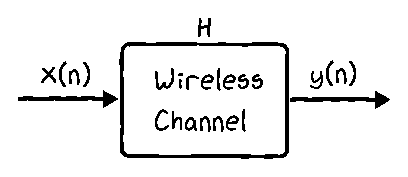
\includegraphics[]{chapters/part_pathloss/figures/adaptive_filter.eps}
\caption{The wireless channel can be seen as a dynamic system. The task at the receiver is to \emph{equalize} the channel conditions, e.g. approximate the response $H$ such that more of the originated signal $x(n)$ can be recovered by $Y = X*H$ thus $X = Y/H$.}\label{fig:adaptive_filter_system}
\end{marginfigure}

A so-called \emph{Weiner filter} is capable of solving such a system. Nevertheless, it requires the so-called inverse auto-correlation, which is computational heavy \cite{Tan2013DigitalProcessing}. More so, the auto-correlation function is based on statistics; therefore, a significant number of samples are required. To combat the complexity of such a filter, an adaptive filter using a \gls{lms} with steepest descent can accurately approximate an optimal filter using iterations. The weights of the filter are updated such that they converge towards the optimum weights. Such a steepest descent can essentially be termed a gradient descent algorithm, which uses the gradient of the error to update the weights. The weight update equation can be seen as
\begin{equation}
    w_{n+1} = w_n - \mu \nabla  \epsilon [n]
\end{equation}

Where $\mu$ is a converging factor, and $\nabla  \epsilon [n]$ is the gradient of the mean-squared error between the output of Eq. (\ref{eq:fir}) and the true observations of the channel. The update equation adjusts the weight by considering the error, and the direction of it. $\mu$ is the step-size of updating the coefficients and is an important parameter for controlling convergence complexity. Updating the weights in this way is essentially the same principle used for updating weights in \gls{nn}. An example of an equalizer applied to a signal in mobile communication can be seen in Fig. \ref{fig:equalizer_example}. The filter successfully corrects phase and amplitude to effectively \emph{cancel out} the imposed channel impairments.

\begin{figure}
    \centering
    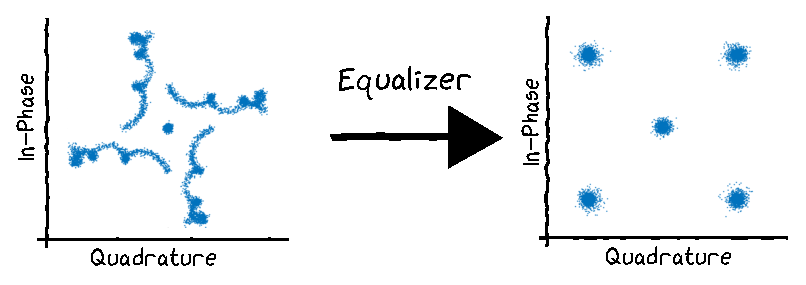
\includegraphics[width=\textwidth]{chapters/part_pathloss/figures/equalizer_example.eps}
    \caption{A received signal under impairments can be seen on the left-hand side. The equalizer is tasked with identifying the channel coefficients through the weight update procedure. The resulting constellation diagram of \gls{qpsk} symbols can be seen on the right-hand side. }
    \label{fig:equalizer_example}
\end{figure}

\subsection{Neural Networks}\label{sec:neural_networks}

Neural Networks are essentially a collection of adaptive weights that are connected, similar to how an \emph{adaptive filter} is constructed. However, one key difference is the use of non-linear transformation functions on said weights (also known as activation functions). \glspl{nn} are highly flexible and is capable of approximating any continuous function in $\mathbb{R}^n$ \cite{Nielsen2015}. This property makes them incredibly useful for many complex problems. The purpose of this section is to provide the reader with basic principles related to \gls{nn}. More details, proofs, and applications can is found in references such as \cite{Nielsen2015}, \cite{M.Bishop2006}.

A two-layer \gls{nn} can be written in the form.

\begin{equation}\label{eq:neural_network}
  y_k(\mathbf{x},\mathbf{w}) = \sum_{j=1}^M w_{kj}^{(2)} h\left( \sum_{i=1}^D w_{ji}^{(1)}x_i+w_{j0}^{(1)} \right) +w_{k0}^{(1)}
\end{equation}

Where $y_k$ is the kth output given a number of inputs $\mathbf{x}$ and a set of weights $\mathbf{w}$, each layer consists of a finite number of weights, in case denoted by $D$ and $M$ for layer (1) and (2) respectively. $h(\cdot)$ can be seen as any transformation function, also termed an \emph{activation} function. The weights are updated using a \emph{loss} function that seeks to compute the error between the predicted $y_k$, and the observed $y_k$. For example, for a single output $y$, with $n$ observations we can write a sum of squares as follows.


\begin{equation}\label{eq:sum-of-squares}
  E(\mathbf{w}) = \frac{1}{2}\sum_{n=1}^N ||y_n(x_n,\mathbf{w}) - t_n ||^2
\end{equation}

In this particular case, the observation is denoted $t_n$. Such a loss function is commonly used when dealing with continuous observations. Different loss function exists for various purposes. However, the principle of minimizing the loss with respect to the weights $\mathbf{w}$ is similar regardless of the loss function used \cite{M.Bishop2006}. For the sum-of-squares error function, as shown in Eq. \ref{eq:sum-of-squares}, it can be shown that maximizing the likelihood function is identical to minimizing the sum of squares. The task is to find a point in the weight space $w$ where the gradient of the error function is zero thus $\nabla E(w) = 0$. However, due to the non-linearities imposed by the function $y_k(\cdot)$ finding an analytical solution is not feasible. For these reasons, the update of weights in \gls{nn} use an iterative approach, much like the adaptive filter. For cohesion, the weight update equation for \gls{nn} in its simplest terms can be written as

\begin{equation}\label{eq:weight_update}
    w_{\tau + 1} = w_{\tau} - \eta \nabla E(w_{\tau})
\end{equation}

In \gls{nn} terms, we can see this as utilizing the gradient information by stepping in the direction of a negative gradient. $\eta$ is known as the \emph{learning rate} and determines the step size. Several techniques for utilizing gradient information exist. The primary difference is related to how large batches of data is iterated over. The two primary principles used throughout this dissertation is:

\paragraph{Stochastic gradient descent}
is also known as an online gradient descent method that seeks to update the weights based on one data point at a time.

\paragraph{Mini-batch gradient descent}
Unlike traditional batch methods such as \emph{steepest descent}, the utilization of mini-batches splits the training set into smaller batches hence \emph{mini-batch}. Mini-batch training has shown to stabilize training and improve convergence time. \cite{Nielsen2015}.

The gradient information is relatively easy to utilize, if and only if, one can compute the gradient with respect to the weights for all weights in \gls{nn}. Even for a two-layered \gls{nn}, a problem arises. It is only possible to measure the error at the output layer; thus, the first layer requires information from the last layer. Here is where the idea of \emph{back propagation} comes into play. Backpropagation is a technique for passing messages backwards through \gls{nn}. It can be shown that by applying the chain rule, we can construct a method for moving around the necessary gradient information. Such a proof can be found in references as \cite{Nielsen2015, M.Bishop2006}. In short, the backpropagation procedure consists of 1) Applying an input to the network and forward propagate the entire network. 2) For all outputs, the derivative of the error is evaluated. 3) the \emph{errors} is propagated backwards such that a derivative is obtained for all hidden units. 
 



\subsection{Training, test and validation}
Learning any model requires separate datasets for training and testing the model to avoid such factors as over and underfitting. If the complexity of the model is higher than what is required for learning the underlying function, it results in learning of the noise present in the dataset instead of the characteristics of the problem, which is usually not desired and is also termed overfitting. If the model is simpler than the function to be learned, the model will not provide effective predictions and is termed underfitting. A comprehensive and detailed introduction to such overfitting and underfitting terms and how it relates to model complexity can be found in \cite{M.Bishop2006}. To test and validate the performance of a trained model the data is split into separate datasets. Some of the data is thus kept unseen to the model when trained. Over time and experiments, it is unavoidable to develop some kind of bias for a particular dataset, regardless of it being seen or not during training. Thus, the more data available, the more validation is possible. A few common tricks of the trade can be used to increase data quantities, such as \emph{data augmentation} (See \ref{sec:regularization}) or \emph{cross-validation}, the objective being the same; improve performance of the model for unseen combinations of features and targets. In other words, separate datasets are required for validating if the underlying characteristics of the problem have been learned and if the model is well-tuned.

\subsection{Optimizers}\label{subsec:optimizers}
Several techniques for gradient descent have been developed over recent years to deal with training issues and improving training speed. A vital concern of traditional stochastic gradient descent is getting stuck in local minima in the cost function space, which restricts the training performance significantly \cite{Goodfellow-et-al-2016}. Optimizers that improve training performance and avoid or can get unstuck from local minima have been used throughout this dissertation, such as Adam, and L-BFGS \cite{Goodfellow-et-al-2016}. 

\subsection{Regularization}\label{sec:regularization}
The common way of reducing over-fitting of trained models is by introducing regularisation. A simple way is by adding a regularisation term to the cost function as given in Eq. (\ref{eq:sum-of-squares}) such that

\begin{equation}
    E(\mathbf{w}) = \frac{1}{2}\sum_{n=1}^N ||y_n(x_n,\mathbf{w}) - t_n ||^2 + \underbrace{\frac{\lambda}{2} \mathbf{w}^T \mathbf{w}}_{\texttt{weight decay}}
\end{equation}

This scales the loss by the weight vector and a parameter $\lambda$ and essentially encourages the weight values to decay towards zero, which has been termed \emph{weight decay} in literature. Several functions for regularisation can be added to the cost function, and such approaches are commonly termed \emph{L1} and \emph{L2} regularisation, depending on the specific term used for the weight decay. However, the purpose is identical, to force or encourage the weights towards zero. However, if too much weight decay is added the issues of under-fitting might arise. It is thus an essential hyper-parameter in the training of any \glspl{nn}.

\paragraph{Dropout}
Regularisation can also be introduced by several techniques directly embedded into the structure of the model. Examples of such layers are, drop-out and batch normalization (See section \ref{subsec:dropout} and \ref{subsec:batch_normalization})

\paragraph{Data Augmentation}
Introducing noise into the data set can also be seen as a regularisation technique as it generates an increase in the quantity of available data. The random noise ensures the model does not memorize the data points as the overall noise present on the observations is increased, which effectively reduces over-fitting and ensures the model converges towards the underlying function capable of characterizing fundamental properties of the data. Such techniques have successfully been applied to image modelling tasks by introducing random rotations on the original input images \cite{Shorten2019ALearning}. Engineering effective data augmentation techniques are considered a challenge for many supervised modelling problems. 

\subsection{Definitions}
The world of \gls{ml} consists of a particular set of terminology. This section will attempt to summarise some of the primary language and notations used throughout the dissertation.

\paragraph{Features}
The term \emph{input} is used interchangeably with \emph{features} to define the variables given to the model. In the world of statistics, such might also be termed predictors or regressors. As a rule of thumb, we define \emph{features} as engineered inputs and is commonly the primary input variable given to classical \gls{ml} methodologies. In \gls{dl}, raw data is processed through deep layered structures to produce \emph{features}. In this case the input variables to \gls{dl} models are by default termed \emph{inputs}. 

\paragraph{Targets}
The terms \emph{target} and \emph{output} are used interchangeably throughout this dissertation. In the world of statistics, this is also known as \emph{response} variables. 

\paragraph{Layers and Depth}
\gls{nn} utilize layers (or hidden layers) to process features and inputs. Layers consist of adaptive weights termed \emph{neurons}. Each layer in \glspl{nn} has thus a certain amount of neurons. A sequence of layers determines the depth and size of the \gls{nn}. In practice, any \gls{nn} with more than two layers is considered a \gls{dnn}, however, used for different purposes and with different inputs \cite{M.Bishop2006}. Thus when refereed to the \emph{depth} of the model, it is the number of sequentially connected layers. 

\paragraph{Generalization}
The term generalization describes how well a trained model is capable of generalizing the underlying characteristics and functions of the problem. In practice, generalization is seen as the gap between training and test losses - also known as the \emph{generalization gap}. 

\subsection{Implementation}
The research of applying and studying \gls{ml} and \gls{dl} methods are contingent on the ease of implementation. Several toolboxes are made available, (either open-source or under license) that ease the efforts required for implementation. For instance, MathWorks, has spent efforts towards designing drag-and-drop \gls{gui} for constructing \gls{dl} models with \gls{gpu} acceleration. that enables the creation of complex models by everyone interested. A few of these toolboxes have been utilized throughout the research documented in this dissertation. Initial models were implemented with Tensorflow \cite{tensorflow2015-whitepaper}. For later and improved implementations, Pytorch \cite{Paszke2017AutomaticPyTorch} was utilized. The Deep Reinforcement Learning was completed using the \cite{MATLABRL_toolbox}. The different implementations do in practice mean different results. However, due to the large communities maintaining these toolboxes, it is believed that performance, regardless of the toolbox used, is comparable. 

\subsection{Evaluation Metrics}\label{subsec:eval_metrics}
The metric of evaluating the training and test loss depends on the model architecture. However, a set of well-known metrics can be used for assessing the performance of the proposed approach. Here $\hat{y_i}$ are the predicted values of the model, while $y_i$ are the true values.

\begin{equation}
    MSE =  \frac{1}{N} \sum_i^N (\hat{y_i} - y_i)^2
\end{equation}

\begin{equation}\label{eq:rmse}
    RMSE = \sqrt{\frac{1}{N} \sum_i^N (\hat{y_i} - y_i)^2}
\end{equation}

\begin{equation}
    MAE =  \frac{1}{N} \sum_i^N |\hat{y_i} - y_i|
\end{equation}


\section{\acrlong{dl} Basics}\label{sec:dlbasics}

\gls{dl} is essentially considered an extension of \gls{ml} and utilize a set of tools and functions for processing raw data. A brief overview of these tools will be given in this section. There is a significant number of resources capable of explaining these functions much better and in improved detail. If the reader requires additional information \cite{Nielsen2015} and \cite{Goodfellow-et-al-2016} are recommended resources. The term \gls{dl} and \gls{dnn} are for the remainder of this dissertation used interchangeably. It is important to note that \glspl{dnn} is a term describing a well-defined toolbox of various computational buildings blocks using \gls{nn} principles, whereas \gls{dl} is a more generic description of a family of models that harness raw data for solving complex problems.

\subsection{Deep Neural Networks}
Or \gls{dnn} in short consists of a large selection of \emph{layers} than can be concatenated to offer various non-linear transformation of inputs. These layers can also be seen as independent building blocks, each with a particular property. The deeply nested structure, cascaded or not, is what define the \emph{deep} in Deep Neural Networks. The purpose of the content in this dissertation is to utilize a set of computational tools for applications in mobile communication networks. More so, the contributions of the dissertation are reduced to the usage and not to optimization and improvements of the tools. The area of \gls{dnn} is extensive and continuously evolving. The content of this section is a brief introduction into a tiny area of \gls{dnn} computational tools. 

\subsection{Convolutions}\label{sec:convolutions}
The performance increase of \gls{dnn} in many areas can largely be contributed to the operation of convolution. Traditional image processing algorithms have shown the usefulness and performance offered by convolutions. This combined with methodologies of \gls{nn} and the use of adaptive weights is what has contributed significantly to the impressive results of state-of-the-art speech recognition and computer vision \gls{dnn} \cite{Goodfellow-et-al-2016}. Such models are also termed \glspl{cnn} due to the importance and success of applying convolutional layers. The operation of convolution enables learning important features from raw data as seen in computer vision tasks \cite{LeCun2015}. There is a slight difference in the regular operation of convolution compared to the traditional operation of convolution

The operation of convolution follows the form.

\begin{equation}\label{eq:convolution}
  s(t) = \int x(a)w(t-a)da
\end{equation}

Here $x$ is the input, and $w$ is the so-called kernel. The kernel is a filterbank of adaptive filters, that is learnable through the use of backpropagation techniques. Convolutional layers are primarily the use of convolutions instead of multiplications as used in regular \gls{nn} layers, however, with a slight difference. The convolutional layers consist of several parameters that can be used to adjust the properties of the convolution. These parameters are briefly explained in this section. All of the terms below are subject to optimization and are considered hyper-parameters.

\paragraph{Filters}
Each convolution is essentially a filter; thus, a convolutional layer is a bank of filters each with a set of parameters. These parameters are then learned through the use of backpropagation. The number of filters used in each convolutional layer can be adjusted and is subject to optimization just like other hyper-parameters. 

\paragraph{Kernel Size (Filter size)}
The kernel size is a term describing how many samples are used in the convolution. For example, if used on a 2D image it determines the number of pixels on which the dot product is computed. 


\paragraph{Stride}
The stride defines the \textit{movement} of the kernel. It determines the number of discrete samples between each convolution. For instance, consider a time-series, if a stride of 2 is used, it corresponds to every 2nd sample of the series. 

\paragraph{Padding}
The combination of kernel size, stride, and dilation may result in a shape of operation that is not compliant with the input series or image. Furthermore, it might be that the edge values of the given input are important. Padding is a term describing the operation of adding zeros to adjust the shape and the size of the input or output. This is to adjust the shape and size of the convolutional layer output given parameters of \emph{kernel size}, \emph{dilation} and \emph{stride}.

\subsection{Pooling}
Pooling is the operation of reducing the dimensionality of the feature maps produced by the prior convolutional layer. Pooling is the operation of modifying the output and create a set of summary statistics of nearby outputs. Several functions can be used for pooling such as \emph{average}, \emph{maximum}, and \emph{minimum}. The function is applied on a set of neighbouring data points, thus effectively summarising the representation of the convolutional layers. Pooling assists in making the resulting representation \emph{approximately invariant} to slight changes in the input \cite{Goodfellow-et-al-2016}.


\subsection{Activation functions}
Activation functions are essentially functions applying non-linear transformation of a given input. The purpose of which is to transform a set of inputs to a set of features that offer information relevant for learning. Several activation functions are commonly used in most \gls{dnn}, such as \emph{sigmoid}, \emph{tanh}. However, \gls{relu} is considered the default activation function due to the simple properties. The linearity of the \gls{relu} function is said to preserve generalization properties of linear models while ensuring the optimization is simple. These are useful properties for very deep and large \gls{dnn}. Furthermore, \gls{relu} ensures that the gradients do not explode and cause instability when learning. However, the use of \gls{relu} can result in a so-called \emph{dying} \gls{relu} where the gradient simply becomes zero and thus offer nothing during backpropagation. By adding a simple linear slope to the negative area of the step function, it provides a small variation required for learning. An example can be found in Fig. \ref{fig:leakyrelu}

\begin{figure}
    \centering
    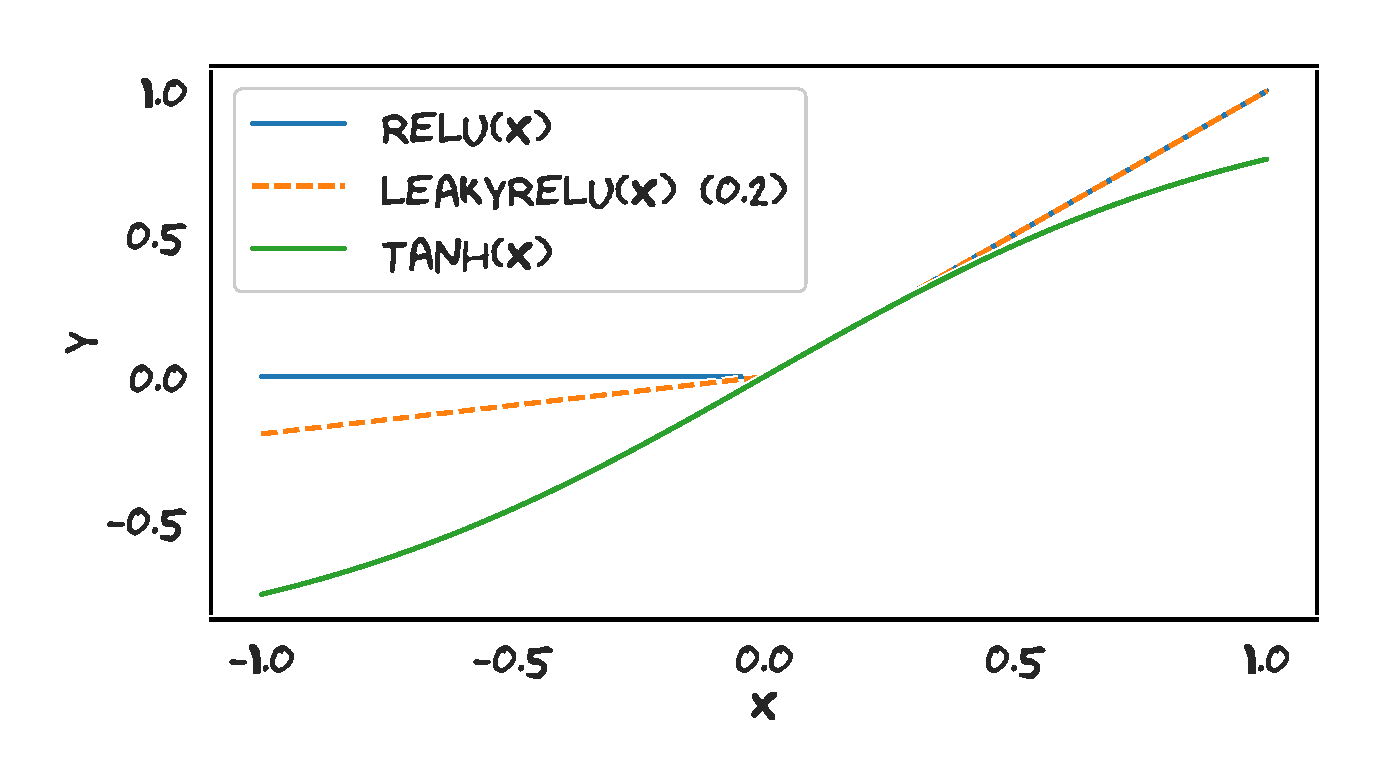
\includegraphics[width=\textwidth]{chapters/figures/relu_leakyrelu_example.eps}
    \caption{Activation output of \gls{relu}, leaky \gls{relu} and tanh.}
    \label{fig:leakyrelu}
\end{figure}


\subsection{Drop-out}\label{subsec:dropout}
Drop-out is a simple method for regularising \gls{dnn}. It is embedded into a layer and acts as a switch for turning off and on nodes. In other words, a probability (usually uniform) is added to all nodes in a layer where drop is wanted. When training, the probability is evaluated causing some nodes to \emph{turn off}. The intuition here is that by turning off some nodes (with some random probability), the combined model does not depend on a specific set of nodes to minimize the loss. This effectively reduces memorization and thus overfitting of the models \cite{Goodfellow-et-al-2016}. Drop-out is the core of the Bayesian approximation method proposed by \cite{Gal2015DropoutLearning}. Very briefly summarised it is utilizing the idea of keeping drop-out layers enabled during testing. By enabling drop-out during testing, an approximation of the posterior distribution can be sampled. The method proposes \gls{mc} sampling of the model, with drop-out enabled, to obtain an approximation of the posterior distribution. The method is based on the idea that overall variance of the underlying problem (given the model is well-tuned) is captured during learning, by the drop-out layers. Understanding the variation when predicting can offer metrics of uncertainty which is extremely useful when dealing with large \gls{dnn}.



\subsection{Batch Normalization}\label{subsec:batch_normalization}
Batch normalization is a key tool in the optimization of \gls{dnn}. The method is considered a so-called \emph{adaptive reparametrization} trick. It reduces the problem of only using the first-order gradient when updating multiple layers which would otherwise only converge using second-order statistics. In basic terms, batch normalization is a set of vectors containing the mean and the standard deviation of the activation output. These vectors are used for normalizing the activation output. Applying this to layers means that learning is stabilized around the distribution of the learning objective and not the expressiveness of the entire network. In other words, the information provided by the first-order gradient might be sufficient in many cases; however, when the \gls{dnn} increase in the number of the layers second-order statistics become non-negligible. Batch normalization improves the training of \gls{dnn} by accelerating it. It can mainly be seen as regularisation tool. It is commonly used instead of drop-out as it has been documented to improve performance in most \gls{dnn} \cite{Goodfellow-et-al-2016}.



\subsection{Upsample/Transposed Convolution}
The components of convolutional layers can effectively apply a set of dimensionality reduction techniques. In some modelling techniques, it is required to scale the resulting dimensionality back to the original input size. A component of building such models is by introducing so-called \emph{upsampling layers} or \emph{transposed convolutions} (also known as a deconvolution). Effectively the output of either method is the same but uses different modes of operation. 


\subsection{Learning Rate scheduler}\label{subsec:lr_scheduler}
The learning rate is a fundamental component of the weight update utilized in backpropagation. As seen from Eq. (\ref{eq:weight_update}) it defines the \emph{step size} of the gradient descent method. When utilizing \gls{dl} models, the weight space in which the gradient is computed tends to be complex. A key issue of training \gls{dl} models (or any \gls{ml} model for that matter) is the presence of local minima. As discussed in section \ref{subsec: optimizers}, the modern optimizers approach this by introducing terms when updating the weight. However, the learning rate is still considered an essential term for the overall weight update. Having too high learning rate effectively results in never reaching the global minima, while having a step size that is too low may result in no convergence within a feasible runtime. Thus, effectively controlling the parameter during training is the purpose of a so-called \emph{Learning Rate Scheduler}. By observing a metric of relevance, the properties of the learning rate can be evaluated while training. One approach is then to notice when no improvements take place during training and lower the learning rate as a result. This is also termed a \emph{Learning Rate Scheduler on Plateau}. An example can be seen in Fig. \ref{fig:learning_rate}, where learning has stagnated and is sequentially reduced.

\begin{figure}
    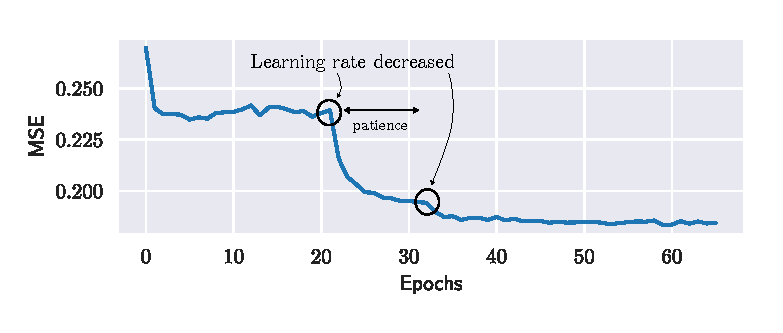
\includegraphics[]{chapters/figures/learningrate_scheduler_example.eps}
    \caption{Example of the training loss with a learning rate scheduler using a patience of 10 epochs before lowering the learning rate. }\label{fig:learning_rate}
\end{figure}

\subsection{Hyper-parameters}

The components of \gls{dnn} consists of many parameters. Such parameters are termed \emph{hyper-parameters} and effectively controls the complexity of the model. Hyper-parameters are fixed and not optimized during regular backpropagation optimization; thus, it is essential to evaluate how a given set of hyper-parameters perform. For the remainder of the dissertation, the notation for a \gls{nn} function $y(\cdot)$ with hyper-parameters is denoted as follows.

\begin{equation}
    t_n = y(x_n, \mathbf{w}, \theta) + \epsilon
\end{equation}

Where $t_n$ is the observation of the learning objective, $x_n$ are the input features, $\mathbf{w}$ are the adaptive weights updated during backpropagation, and $\theta$ denote the used hyper-parameters. An example of such hyper-parameter is the number of samples used in a pooling operation or the number of convolutions applied in the convolutional layer. Deep models are thus exposed to many tun-able parameters and require extensive experimentation to discover optimized hyper-parameters.

Fortunately, the world of computer science is exposed to a particular type of engineers that has the desire to automatize as many tasks as possible, which is also the case for discovering hyper-parameters. Principles of \gls{ml} and in general pattern recognition has successfully been applied to the discovery of the optimum hyper-parameters. Conventional methods include regular exhaustive grid search, random search and the more intelligent Bayesian Optimization which utilize Gaussian Process regression techniques \cite{YuHyper-ParameterApplications}. All of the said methods have been utilized throughout this dissertation.

Regardless of hyper-parameter optimization techniques, the training is still time-consuming. Thus it is necessary to consider relevant early-stopping criteria. Such approaches will be detailed later on for the specific applications.


\subsection{Implementation}
This section has contained some of the many components used in \gls{dnn}. The field is continuously evolving with new and improved methods for not only the processing of raw data like convolutional layers but also optimizers and methodologies for regularisation.  Implementing the state-of-the-art algorithms and structures is a time-consuming affair; however, several open-source libraries ensure that implementation is access-able to any enthusiast. In particular, a few libraries are considered the default selection, the most popular ones are 

\begin{itemize}
    \item TensorFlow \cite{tensorflow2015-whitepaper}
    \item PyTorch \cite{Paszke2017AutomaticPyTorch}
\end{itemize}

Both libraries are mostly a set of highly efficient low-level code written in the \texttt{C}- and \texttt{CUDA}-language. Ensuring ease of implementation is achieved by the abstraction of using the high-level language \texttt{python}. Both libraries enable standard components but also \gls{gpu} acceleration. TensorFlow is a long-standing library maintained by Google, but in recent years PyTorch (supported by subparts of Facebook) has seen an incredible rise in popularity due to the flat and transparent \gls{api} architecture. TensorFlow is not only a \gls{dl} library; it is an extensive collection of computational resources with deployment tools for production environments. The Pytorch library lacks most of these functionalities; however, the ease of implementation greatly out-weighs the benefits offered by TensorFlow. Both libraries have been utilized for the algorithm development in this dissertation. 

\section{Data needs}

Use of any learning algorithm requires data and observations. However, differences in the fundamental learning process (i.e. the family of the adaptive model) requires different kinds of data. For instance, supervised learning (as used predominantly throughout this dissertation) need large quantities of data when utilizing deeply nested models such as \gls{dnn}. Also, depending on the difficulties of the problem, the quantities of data may vary significantly. Obtaining such data is the first bottleneck to overcome. The fundamental properties of the chosen adaptive models put forward a different set of data requirements, and an overview of such requirements can be found in work such as \cite{RohAPerspective}. For example, acquiring necessary labels used for the classification of images is exhaustive and time-consuming, which has consequently lead to the rise of \emph{semi-supervised} approaches. Such methods use tricks and techniques to effectively improve the quantities of data without the need for obtaining additional. The authors show the pressing need for accurate and scalable data collection techniques, which is furthermore enabled by the promise of utilizing \gls{dl} for solving complex tasks. 

The expressiveness of the constructed models furthermore dictates the data requirements. In the case of complex models, the number of parameters and adaptive weights can easily surpass that of the available data points. The resulting models will fit to the observation noise, which is the definition of overfitting. If the data quantities are not constrained, proper regularisation is a necessity to find the optimal model complexity. 

Adaptive models associated with so-called \emph{Reinforcement learning} does not require massive data sets. It, however, requires integration with the actual system in which the problem or optimization task is present. Development of such a combination is time-consuming to engineer and must consider stringent requirements on not only latency but also processing power. Such requirements are usually a bottleneck for the integration of \emph{Reinforcement learning} solutions into real-world systems. For such reasons, simulation and emulation environments are essential for the future of \emph{reinforcement learning}. 

The methods and approaches used for obtaining the necessary data in order to apply the tools of \gls{dl} effectively are put forward in chapter \ref{ch:monster}. 

\section{Summary}
The world of \gls{ml} is massive. The toolbox is so deep and continually evolving that it is expected to get lost somewhere. However, a few terms and principles are expertly maintained and are regularly relevant for state-of-the-art algorithms. The content of this chapter is a brief introductory effort into the world of not only \gls{ml} but also \gls{dl}. To not further confuse the reader the content can be summarised to the following items

\begin{itemize}
    \item Adaptive models is a proven and necessary part of mobile communication systems. The basic principles of these models share the fundamental properties with Neural Networks. 
    \item Neural Networks is a powerful modelling technique that learns through cascaded structures of adaptive weights and non-linear transformations.
    \item \gls{dl} is a subfield of \gls{ml} that primarily utilize \gls{nn}-methodologies and definitions to process and learn from raw data.
    \item Open-source \emph{implementations} are paramount to the development of novel solutions.
    \item Data is the catalyst for novel \gls{dl}-based solutions.
\end{itemize}

\epigraphhead[350]{.}
\part{Estimation of invisible waves}
\chapter{Wireless propagation models}\label{ch:channelmodellingbasics}

The propagation of waves in any medium can be modeled using fundamental principles of physics. It has been shown that the fundamental understanding of these physics are quite accurate and can provide any researcher with a satisfactory knowledge of how waves propagate in air. Wireless transmission is essentially electromagnetic radiation from a transmitter to a receiver. We have the well known \emph{Maxwell} equations for calculating the electromagnetic fields that is received. From such equations it can be seen that as distance $r$ increases the electric field decreases with $r^{-1}$. This means the power of the field decreases by $r^{-2}$ given a sphere is radiating. This is only if we assume the surface area of such a sphere increase as $r^2$ \cite{Tse2005FundamentalsCommunication}. Such a notion is only relevant in free space propagation situation where no reflections are happening, which in the world of mobile communication systems is not typical. Even a very simple situation (such as a reflecting wall and a moving antenna) can be shown to significantly change the profile of the electromagnetic field and its power. This is due to patterns of constructive and destructive interference. This is also known as multipath fading, thus signals can propagate along different paths but arrive at the same time cancel (effectively) each other out. In practice many obstacles are present in a transmission scenario, which means that the power at the receiver decreases with distance much faster than $r^{-2}$. At large distances such a decay is exponential-like. The modelling of this decay in practical transmission scenarios (and the nature of it) is the purpose of this chapter.

Obstacles in the transmission scenario cause signal attenuation as power is absorbed and scattered. This phenomenon is known as shadowing, and can be seen as obstacles blocking (or partly block) the dominant paths of the traversing radio waves. The attenuation of a signal is thus varying over time and frequency, but also determined largely by the obstacles in the radio environment. This complex function of attenuation is normally and regularly described using two key terms, \emph{slow} and \emph{fast} fading. Also termed, Large-scale or Small-scale fading respectively. Both have been studied extensively and can be modeled using statistical and geometric principles.

\paragraph{Large-scale fading}
also known as \emph{slow} fading, is the product of obstacles shadowing the signal. This can also be seen as a change in the number of scatters for a receiver in a given position $x,y,z$. In other words, such obstacles change the paths and reflections of the radio waves which cause spatially determined fluctuations of attenuation at the receiver. 


\paragraph{Small-scale fading}\label{sec:small_scale_fading}
also known as \emph{fast} fading, or just \emph{fading} \cite{Rappaport:2001:WCP:559977} is the effect of interference between several verions of the transmitted wave arriving shifted in time. This is caused by obstacles in the propagation environment causing reflections thus the waves arrive from many directions and with different propagation delays. A large quantity of factors influence small-scale fading such as multipath propagation, the speed of the mobile, the speed of surrounding objects and the bandwidth of the signal. A comprehensive description of small-scale fading can be found in \cite{Rappaport:2001:WCP:559977}. 


\section{Established methodologies for received power estimation}
The received power is determined not only by the impairments and path losses associated with the wireless channel. Several other items have an impact on the final received power. Modelling the final received power is commonly done through the use of so-called link budgets. The link budget is an essential part of designing reliable communication systems and can give insights in the needed requirements of the hardware composing the communication system \cite{Molisch2007}.


\begin{equation}\label{eq:link_budget}
    P_{rx} = P_{tx} + G_{tx} - L_{tx} - L_{PL} + G_{rx} - L_{rx}
\end{equation}

Here $P_{rx}$ is the received power, $P_{tx}$ is the transmitted power, $G_{tx}$ and $L_{tx}$ are gains and losses associated with the transmitter. $G_{rx}$ and $L_{rx}$ are gains and losses associated with the receiver and finally, $L_{PL}$ are the path losses. The complete estimation of received power consists thus of a multitude of terms. In most cases gains and losses of both the receiver and transmitter components can be quite accurately approximated through calibration procedures  \cite{Molisch2007}. The above link budget is rather simplified for use in mobile communication systems and should contain many more parameters to accurately predict received power. In any case the most attenuation of the link budget is associated to path losses, thus predicting and estimating accurate path losses is the most essential element. Unfortunately the task of estimating accurate path losses are either 1) computational complex to ensure high accuracy or 2) computational fast but at the cost of inaccurate estimations. Models for obtaining path loss estimations are from hereon termed \emph{wireless channel models} or just \emph{channel models}. However, it is important to note that wireless channel models must consider not only power but also delays and other components. A complete overview of wireless channel models will not be given in this dissertation, and the reader is refereed to the content of common textbooks such as \cite{Tse2005FundamentalsCommunication}.

Obtaining approximations of $L_{PL}$ is challenging and many approaches for doing so have been developed over the existence of mobile communication systems. Channel models for wireless transmission have been subject to much research and are seperated into two fundamental \emph{families} of channel models. Such families are either considered \textbf{statistical} or \textbf{geometric}. This chapter will outline the purpose and properties of various existing channel modelling methodologies. This is necessary in order to motivate and visualize where learning methods could improve the current methodologies.

\begin{figure}[thbp]
    \centering
    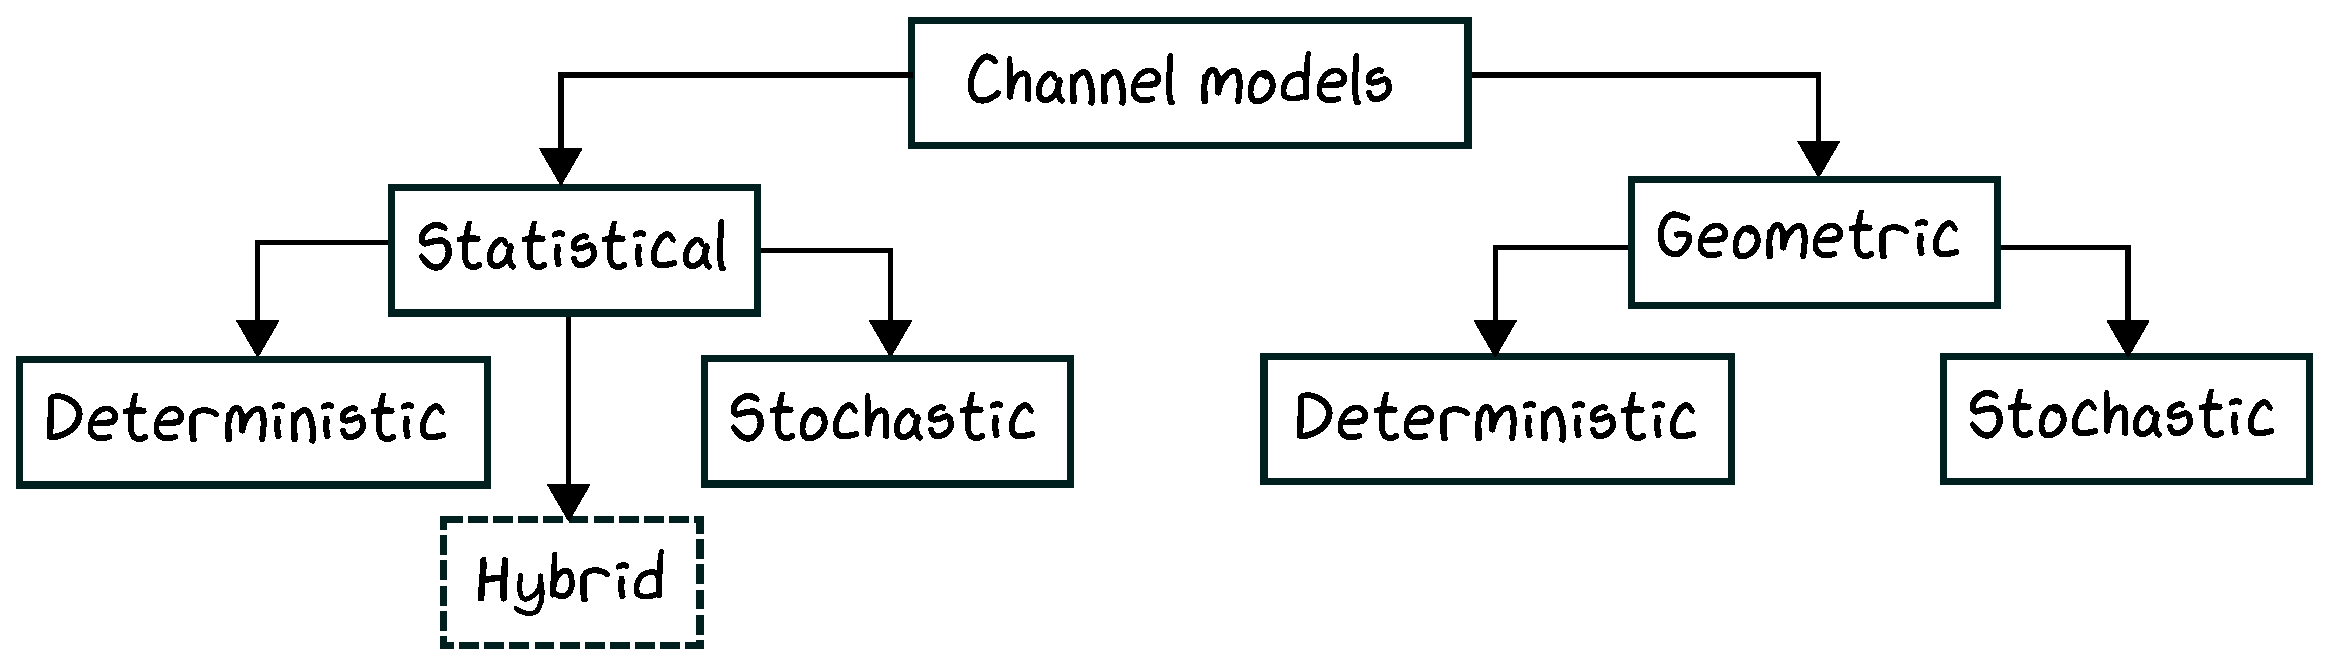
\includegraphics[width=\textwidth]{chapters/part_pathloss/figures/channelmodel_tree.eps}
    \caption{Two \emph{families} of channel models have been the default approach for modelling the wireless transmission impairments. Each of the families, statistical and geometric deal with both deterministic and stochastic approaches. Recently hybrid methods have gained attention for improving accuracy while keeping valuable statistical properties.}
    \label{fig:channel_models}
\end{figure}


\subsection{Statistical}
By obtaining measurements of radio propagation, the resulting statistics can be studied and exploited for estimating path loss. This is the basis of so-called \emph{statistical channel models}, also termed \emph{empirical models}. The use of statistical methods have a long standing history due to the simplistic required analysis. The variations of path loss can furthermore be described with additional statistics in a stochastic setting. For instance, the variations provided by large-scale fading impairments have been found to be representative with a log-normal distribution. The parameters of the distribution is then propagation scenario dependent. Additional approaching for utilizing such statistics can be found in Section \ref{sec:stochastic_channel_model}.

Analysing the statistics of radio propagation measurements is a practical way of obtaining effective approximations of the radio channel. However, it can also be understood that engineering statistics to cover all possible transmission scenarios is simply not feasible. For such reasons the statistical methods turn to stochastic approaches which can offer valuable margins for further link budget analysis. In some well defined propagation scenarios a set of deterministic features enable increased accuracy in path loss estimation which have sparked hybrid models. These hybrid models mix very specific propagation statistics with a stochastic representation of any variations in the path loss. 

Statistical methods is a classical way of providing path loss estimations using regression techniques. A brief introduction to such models can be found in Section \ref{sec:empirical_path_loss}.


\subsection{Geometric}
In practice radio propagation can be described as the propagation of \emph{radiowaves} through electromagnetic radiation. This can in a theoretical and mathematical setting be reduced to the idea of the waves taking certain \emph{paths} determined by the objects in the propagation environment. Geometric models is the study and thus approximation of how the radiating radiowaves will propagate throughout the given propagation scenario. This is reduced to computing the most dominant and likely paths the signal will traverse \cite{Tse2005FundamentalsCommunication}. In essence the result of doing so is in principle an approximate solution to utilizing Maxwell's equations. Geometric channel models are based on these principles and can be reduced to a deterministic and stochastic representation.

Ray-tracing is a deterministic way of computing the dominant and likely paths in a propagation scenario by assuming a finite number of reflectors. However, such channel models require detailed information of objects present in the propagation environment, which can be a significant bottleneck in the creation of such models. Example of ray-tracing models and the resulting accuracy are given in Section \ref{sec:ray-tracing}.

Geometric stochastic models consists of representing so-called \emph{scatterers} in the radio environment by using not only distributions of spatial location, but also the distributions of the resulting angle of propagation. Such models are essential for the study and simulation of realistic \gls{mimo} transmission.  

\section{Empirical path loss models}\label{sec:empirical_path_loss}

One of the earliest examples of such a model is the Free-space path loss model \cite{Goldsmith2005WirelessCommunications}. However, as noted earlier models assuming free-space struggle in outdoor propagation scenario with the presence of many objects and the resulting obstruction of transmission. One of the earliest examples of a path loss model derived and calibrated for urban propagation statistics is the Okumuara-Hata propagation path loss model \cite{Hata1980}. The authors showed that a model with simple parameters is capable of predicting path loss with satisfactory accuracy using a function of distance. The field strength can be described as a function of distance ($R$) following the form
\begin{equation}
    L(dB) = A + B \log_{10} R
\end{equation}

\begin{marginfigure}
    \centering
    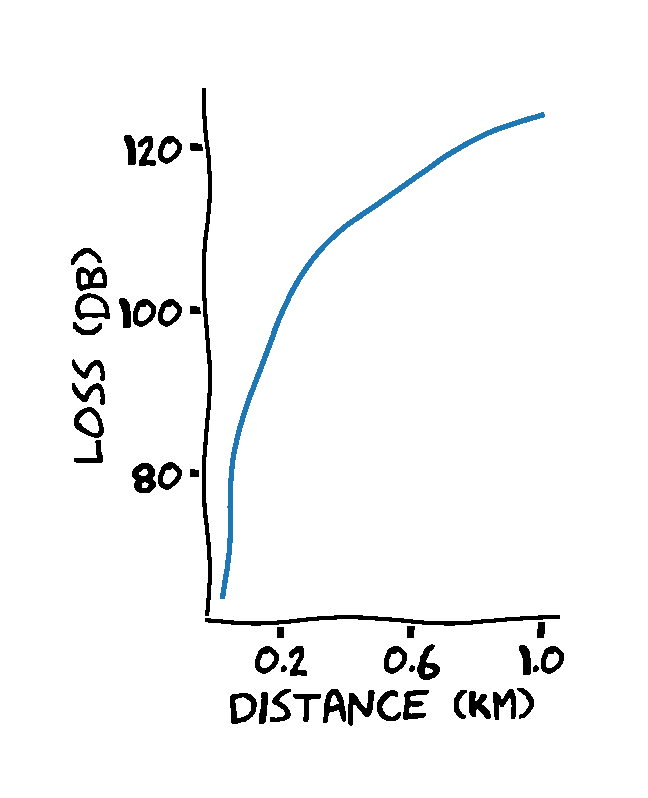
\includegraphics{chapters/part_pathloss/figures/okumura-hata-pathloss.eps}
    \caption{The Okumuara-Hata path loss model and the exponential decay of attenuation related to distance.}
    \label{fig:my_label}
\end{marginfigure}

Where $A$ and $B$ are correction factors that account for characteristics of the propagation scenario, such as the transmitter/receiver antenna height and the frequency. Such parameters, $A$ and $B$ was derived using field measurements in an attempt to \emph{generalize} the propagation characteristics. It has ever since been validated to be a simple and effective approach of estimating losses related to distance of transmission. A few corrections to the original models have been made over the years which has resulted in new measurement studies. These studies have paved the way for more accurate path loss models that is capable of generalizing more propagation scenarios.

Significant efforts have been spent in an attempt to achieve empirical path loss models that generalize well. This is illustrated by the recent technical documents as proposed by \gls{3gpp} and \gls{itu}. In particular, the documents of interest are titled

\begin{itemize}
\item \textbf{\gls{3gpp} TR 38.901 - \cite{3GPP38901}} - Study on channel model for frequencies from 0.5 to 100 GHz
\item \textbf{\gls{itu}-R M.2412 \cite{ITU2412}} - Guidelines for evaluation of radio interface technologies for IMT-2020
\end{itemize}

In both sources a detailed process for the modelling for radio propagation for mobile communication networks is supplied and summarized. The content of both documents are thus considered the default approach for modelling the wireless channel in mobile communication systems per \gls{lte} and \gls{nr} deployed solutions. The content of both documents are rather vast, a focus on the modelling of mean path loss using the empirical models under shadow-fading impairments are given below.

\subsection{Propagation scenarios under consideration}
Inherently different settings of propagation. An attempt to generalize the amount of obstacles and overall propagation characteristics of a given propagation scenario. For example, as defined by \gls{3gpp} in \emph{38.901} are three distict propagation scenarios, each considering different statistics. 

\begin{itemize}
    \item \gls{rma}
    \item \gls{uma}
    \item \gls{umi}
\end{itemize}

For the case of ITU-R M.2412 \cite{ITU2412} a few additions are given. Moreover, such additions are defined as \emph{test environments} for IMT-2020 and are as follows
\begin{itemize}
    \item Indoor-\gls{embb}
    \item Dense Urban-\gls{embb}
    \item Rural-Indoor-\gls{embb}
    \item Urban Macro-\gls{mmtc}
    \item Urban Macro-\gls{urllc}
\end{itemize}

Such environments does not only define a path loss models, but also more specific transmission configuration parameters along with more general network configuration parameters. For example, each of the listed test environments consider specific configurations of \gls{ue} density. A large selection of configuration details for each of the test environments can be found in \cite{ITU2412}.


The title of the \gls{3gpp} document makes the point quite clear. Having channel models that are capable of generalizing losses in the frequency range of 0.5 to 100 GHz. A complication of state of the art measurements campaigns have been utilized in both documents, and the share many similarities. Without summarizing the entirety of the documents, the main differences (in terms of path loss models) can be outlined as:

\begin{itemize}
\item M.2412 offers:
\begin{itemize}
\item \gls{inh}\_A, \gls{inh}\_B
\item Dense urban: \gls{uma}\_A, \gls{uma}\_B, \gls{umi}\_A, \gls{umi}\_B
\item Rural: \gls{rma}\_A, \gls{rma}\_B
\end{itemize}
\item \gls{3gpp} 38.901
\begin{itemize}
    \item Indoor: \gls{inh}
    \item Urban: \gls{uma}, \gls{umi}
    \item Rural: \gls{rma}
\end{itemize}
\end{itemize}

Thus, M.2412 offers models termed $A$ and $B$. The difference is related to the carrier frequency ($f_c$). Models termed $A$ is for a frequency range of $0.5\; \text{GHz} \leq f_c \leq 6 \;\text{GHz}$. Whereas $B$ is for $0.5 \; \text{GHz} \leq f_c \leq 100 \; \text{GHz}$. In relation to 3GPP TR 38.901 this is slightly different. The ITU model termed $B$ is identical (and based on the same channel measurement campaigns) to that of 3GPP 38.901. A \gls{los} and \gls{nlos} model exist for all propagation scenarios. The modelling of the \gls{los} state is similar for both documents and is briefly outlined in section \ref{subsec:los}.

\subsection{Recent empirical path loss models}

In \gls{3gpp} TR 38.901, attenuation for an Urban Macro scenario (\gls{uma}), given a \gls{nlos} transmission state is defined as

\begin{equation}\label{eq:uma_nlos_pathloss_max}
     PL_{UMa-NLOS}^{'} = \text{max} \left( PL_{UMa-LOS}, PL_{UMa-NLOS}^{'} \right)
\end{equation}

Where

\begin{align}\label{eq:uma_nlos_pathloss}
\begin{split}
     PL_{UMa-NLOS}^{'} &= 13.54+39.08\log_{10}(d_{3D}) \\
      &\quad+ 20\log_{10}(f_c) - 0.6(h_{UT}-1.5) \\
  \end{split}
 \end{align}

Additionally, it uses the \gls{uma} \gls{los} model, $PL_{UMa-LOS}$. The loss in the \gls{los} model is dependent on a so-called \emph{breakpoint} distance which essentially turns the path loss function into to a multistep path loss function. The breakpoint distance is defined as $d_{bp} = 4 h_{BS} h_{UT} f_c / c$. In summary, the empirical model is a factor of the following parameters: $\mathbf{h_{BS}}$ (Base station height), $\mathbf{h_{UT}}$ (User terminal height), $\mathbf{d_{3D}}$ ($3$D distance), and $\mathbf{f_c}$ (Carrier frequency). The \gls{3gpp} path loss models can be found in \cite{3GPP38901} Table 7.4.1-1. 

The \gls{rma} model utilize additional parameters of $\mathbf{h}$ (average building height) and $\mathbf{W}$ (average street width).

% \begin{align}\label{eq:rma_nlos_pathloss}
% \begin{split}
%     PL_{RMa-NLOS} &= 161.04-7.1\log 10( W) + 7.5 \log 10(h) \\
%      &\quad- (24.37 -3.7*(h/h_{bs})^2)\log 10(h_{bs}) \\
%      &\quad+(43.42 - 3.1\log 10(h_{bs}))(\log 10(d_{3D})-3) \\
%      &\quad+20\log 10(f_c) - (3.2(\log 10(11.75h_{UT}))^2 - 4.97)
%  \end{split}
% \end{align}

\subsection{Stochastic modelling of impairments}\label{sec:stochastic_channel_model}
The complete budget of attenuation related to transmission can be modeled as a \emph{\textbf{statistical and stochastic process}} by introducing terms for fading. More specifically, terms for Large-scale fading and Small-scale fading. Parameters related to these phenomenons are termed \gls{lsp} and \gls{ssp} respectively. It has been shown that the overall loss can be modeled as described

\begin{equation}\label{eq:pathloss_model}
  PL(d,t) = L(d) + X_\sigma + L(t)
\end{equation}

Where $L(d)$ is the mean path loss, for instance the \gls{uma} model as seen in Eq. (\ref{eq:uma_nlos_pathloss_max}), $X_\sigma$ is shadow fading and $L(t)$ is small-scale fading. Guidelines and parameters of both the large- and small-scale terms are given in the \gls{3gpp} and \gls{itu} documents. The amount of parameters are quite significant thus only a small selection of principles, methodologies and parameters are included in this dissertation. 

\begin{figure}
    \centering
    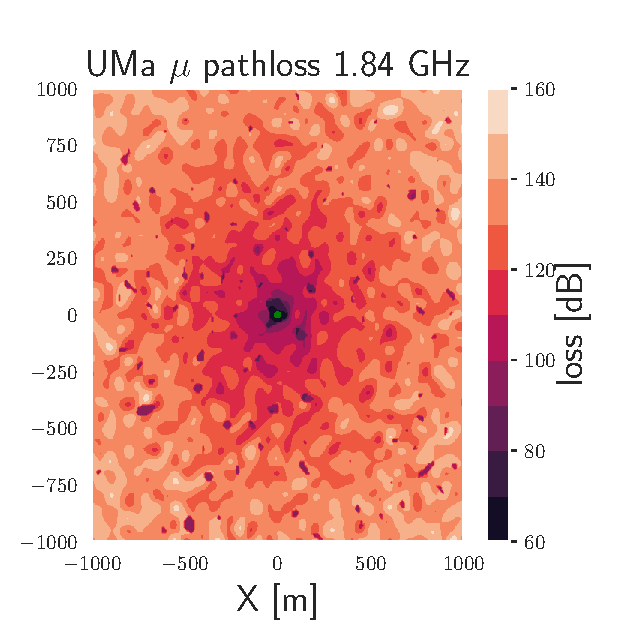
\includegraphics[width=0.6\textwidth]{chapters/part_pathloss/figures/UMaPL.eps}
    \caption{Example of Eq. (\ref{eq:pathloss_model}) for a time-invartiant channel with spatial consistency.}
\end{figure}


\subsection{Shadow fading}
\begin{figure}
    \centering
    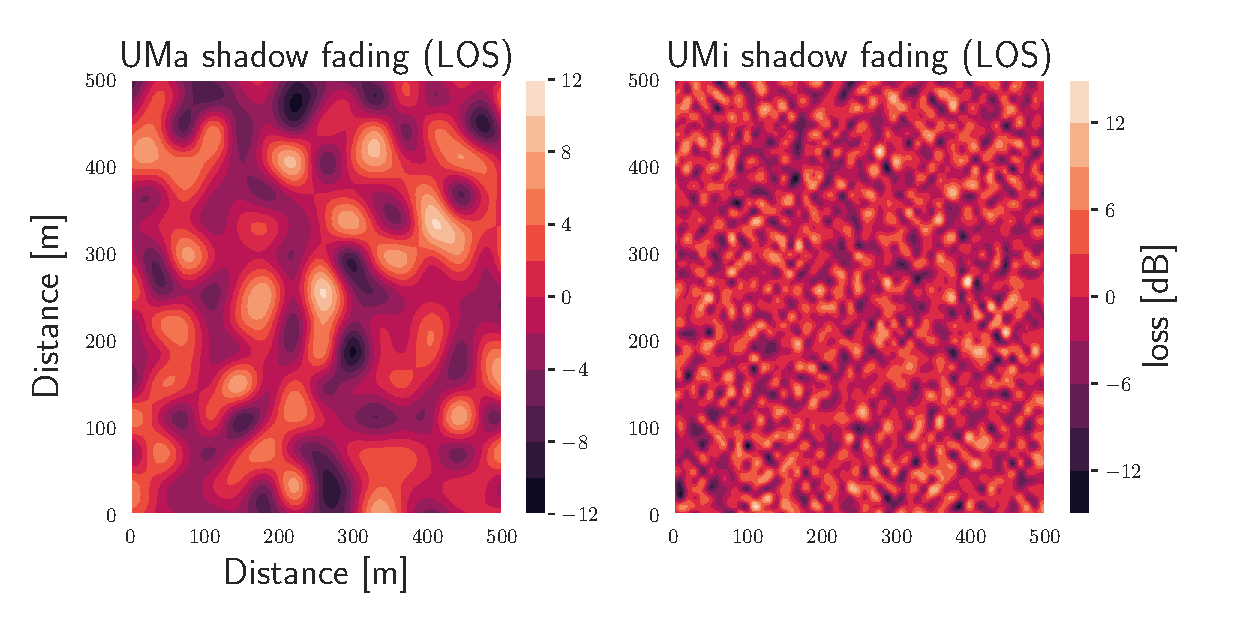
\includegraphics{chapters/part_pathloss/figures/UMaUMiShadowFadingMapLOS.eps}
    \caption{Example of shadowing fading magnitude maps in x,y coordinates with spatial consistency for \gls{uma} and \gls{umi}.}
    \label{fig:uma_umi_shadow_fading_example}
\end{figure}

    
As noted eariler, large-scale and more specifically shadow fading is well represented by a log-normal distribution. Thus $X_\sigma \sim \mathcal{N}(\mu, \sigma^2)$ is a log-normal distribution with mean zero and a variance determined by $\sigma$. The magnitude of $\sigma$ is dependent on the propagation scenario, for instance \gls{uma} or \gls{rma}. The variance of the distribution dictates the variability of the shadowing impairments and is also known as \emph{local variability} \cite{Perez-Fontan2008}. The magnitude of shadowing is determined using measurement studies, such as the one seen in \cite{Sun2016}. The studies mentioned in the fore mentioned work is used as a baseline for the models proposed and defined in \textit{\gls{3gpp} 38.901}. An example of the standard deviation, i.e. the magnitude of shadowing in dB can be observed in Table \ref{tab:sigma_SF} for each of the defined propagation scenarios.


\begin{table}[b]
    \centering
    \begin{tabular}{@{}ll@{}}
    \toprule
    Scenario   & Shadow fading std (dB)               \\ \midrule
    RMa (LOS)  & $\sigma_{SF} = 4$, $\sigma_{SF} = 6$ \\
    RMa (NLOS) & $\sigma_{SF} = 8$                    \\
    UMa (LOS)  & $\sigma_{SF} = 4$                    \\
    UMa (NLOS) & $\sigma_{SF} = 6$                    \\
    UMi (LOS)  & $\sigma_{SF} = 4$                    \\
    UMi (NLOS) & $\sigma_{SF} = 7.82$                 \\ \bottomrule
    \end{tabular}
    \caption{Shadow fading magnitude from \cite{3GPP38901}.}\label{tab:sigma_SF}
\end{table}


However, it is also important to note that such distributions have a so-called \emph{decorrelation distance}. This is to ensure spatial consistency between the magnitude of shadowing effects. In other words, obstacles causing the shadowing are likely spatially dependent and thus users moving with a region of the propagation space will experience the same magnitude of shadowing. This is also illustrated in Fig. \ref{fig:shadowing_decorrelation_distance}. The magnitude of shadow fading can be seen as a Gaussian distribution around the mean estimated path loss. The \emph{decorrelation distance} is then the distance between each Gaussian distribution. In practice this can be seen as the shadow fading effects not being sudden, but rather a function of objects surrounding the receiving antenna. If the receiving antenna is to move slowly the shadow fading does not change immediately but related to the so called decorrelation distance. In other words, the decorrelation distance is a term to seperate the objects in the environment that cause and create the shadowing effect. Shadowing a complex function of interactions but it has been found that utilizing such a decorrelation distance is a good approximation. However, it is important to consider also spatial consistency when modelling these impairments.


\begin{figure*}[h]
    \centering
    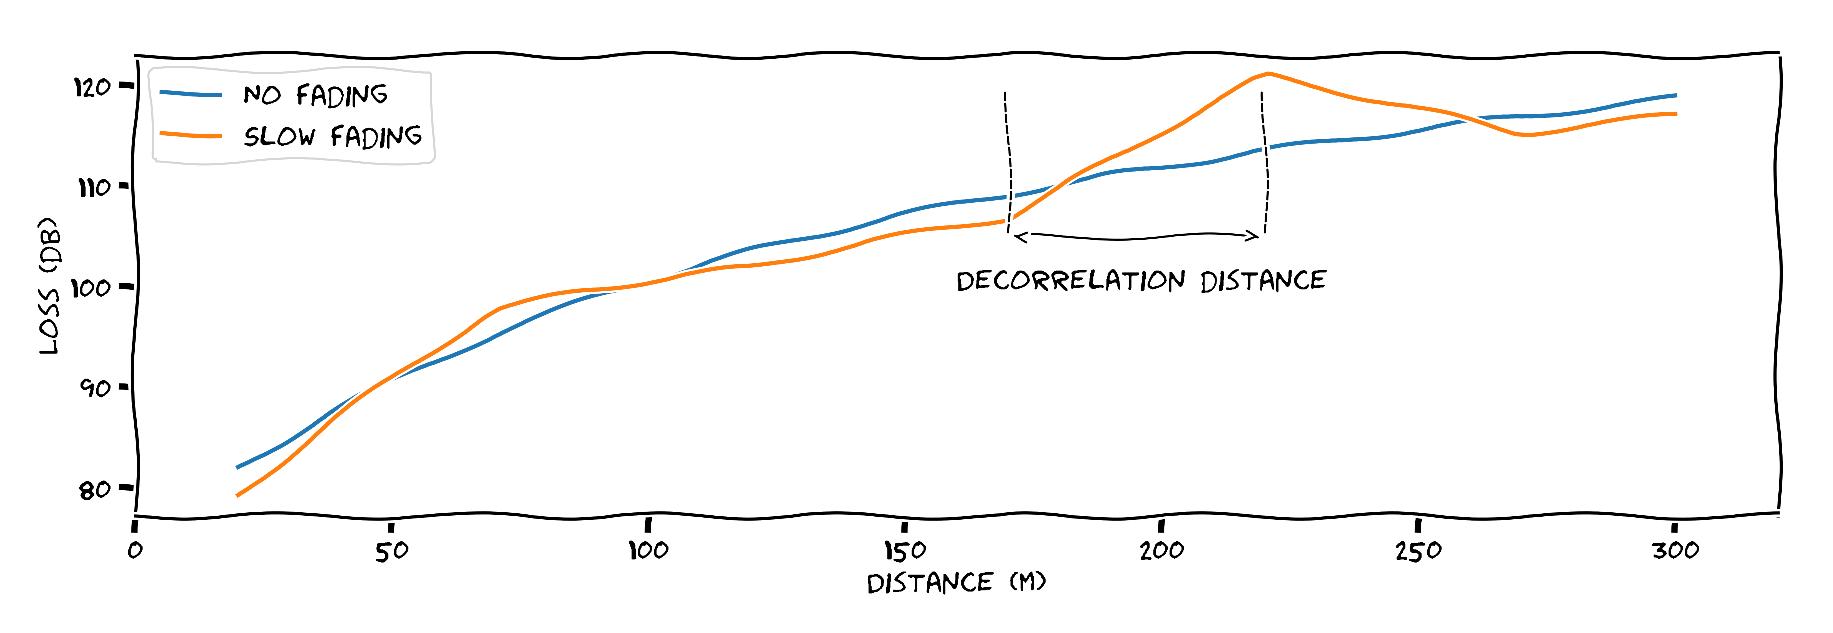
\includegraphics{chapters/part_pathloss/figures/slowfading.eps}
    \caption{Large scale fading, also known as slow fading is the effect of obstacles shadowing the signal. When a receiver moves  the magnitude of such fades change. The distance at which the magnitude changes can be described as a \emph{decorrelation distance}.}
    \label{fig:shadowing_decorrelation_distance}
\end{figure*}



\paragraph{Spatial consistency}
Positions close to one another share common propagation properties, thus it is reasonable to assume that fading impairments have some decorrelation distance. However, in a radio environment this distance needs to also consider a directionality. What this means is that shadow fading is not only dependent on a distance between the fading phenomena but rather dependening on a position with the radio environment. In short, the modelling of shadow fading should consider positions within a space rather than a single distance metric. This results in a necessary translation to 2D coordinates. An example of such a constructed map of shadow fading can be seen in Fig. \ref{fig:uma_umi_shadow_fading_example}.


The figure is produced utilizing a simple procedure as follows 1) realised Gaussian distributions for $N$ points in the grid with a decorrelation distance, and 2) a 2D filtering technique to interpolate values between the realised Gaussian distributions. The number of normal distributions to realise in a position grid is thus given by limits in the X and Y axis and the resulting decorrelation distance. Meaning, for each distance in x and y space, a Gaussian distribution is realised. This results in an incomplete and sparse map which is then 2D filtered.

The large-scale parameters is not only the consideration of shadow fading. More exists with seperate decorrelation distances, meaning the 2D map turns into a multidimensional map of realised distributions. This is computionally infeasible using standard 2D filtering techniques. Using a set of matrix factorization techniques such as the Cholesky factorization the map can be computed while limiting the memory usage and keeping the computational complexity low.


\subsection{Small-scale fading}
\begin{figure}
    \centering
    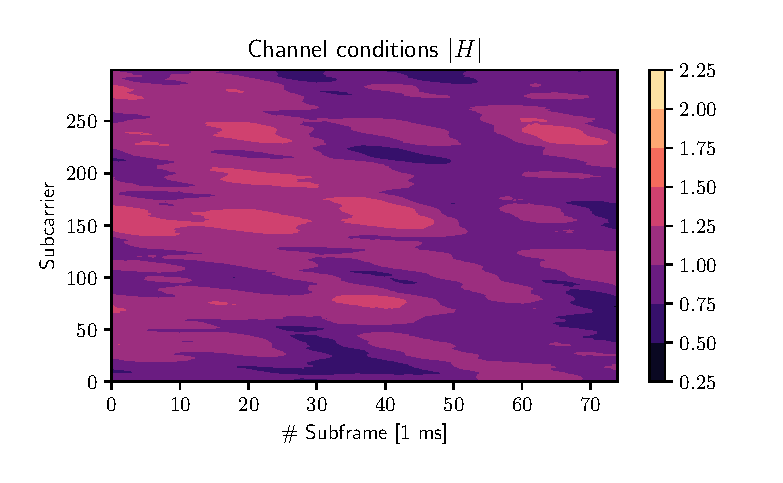
\includegraphics{chapters/part_pathloss/figures/fast_fading_example.eps}
    \caption{Example of the \texttt{\gls{tdl}-E} model at $6$ GHz for $300$ subcarriers.} 
    \label{fig:fast_fading_example}
\end{figure}


The modelling of small-scale fading (or \emph{fast} fading) is more relevant for the immediate design of reliable and efficient communication links. More specifically, fast fading margins is something that is commonly added to link budgets, but, due to the fast varying nature of it; mobile communication systems are unlikely provisioned with respect to this margin. It is something to be considered, but not something that determines cell-site locations and solutions for coverage holes. Here large-scale fading is more relevant. Regardless, the modelling of small-scale fading is paramount to the development of efficient \gls{mimo} solutions and the timing constrained subsystems of mobile communication systems. Common distributions for modelling these impairments include, Rayleigh and Rician.

Since the documents from both \gls{3gpp} and \gls{itu} offer also geometric stochastic models, the modelling of fast fading impairments can be done in several ways. For non-\gls{mimo} study scenarios two models are found in the 38.901 document. More specifically, a so-called \gls{cdl} and \gls{tdl}. A \gls{tdl} model is a common and efficient way of implementing the cause of fast fading i.e. the multi-paths of the channel. The general notion is the implementation of multiple so-called flat-fading generators that are independent. Flat-fading meaning they are not frequency dependent. The implementation is done as a \gls{fir} filter with specific number of taps, each of which have a specific delay (in time),  power attenuation (in dB) and Doppler information. Table 7.7.2-1 in \cite{3GPP38901} describes the delay profile for the so-called \gls{tdl}-A model. The \gls{cdl} model is an extension of the \gls{tdl} model that considers reduced variability and fixed parameters \cite{ITU2412}. An example of the absolute channel coefficients using the \gls{tdl}-E model can be seen in Fig. \ref{fig:fast_fading_example} over time and frequency. 


% Example maybe?

\subsection{Line-Of-Sight}\label{subsec:los}
From the path loss models, e.g. Eq. (\ref{eq:uma_nlos_pathloss_max}) it can be noted that \gls{los} and \gls{nlos} states exists. Determining \gls{los} can be a tricky endavour in outdoor propagation scenarios situations for mobile communication systems. Therefor, the \gls{los} can be modeled in a stochastic manner, using a probability distribution that can be approximated by distance from the transmitter and the height of both the receiver and transmitter antenna. An example of \gls{los} probability can be seen in Fig. \ref{fig:los_probability}. It shows that distances within $20$ meters have $100\%$ of being within \gls{los}, and decreases exponentially given the distance to the transmitter. 

\begin{marginfigure}
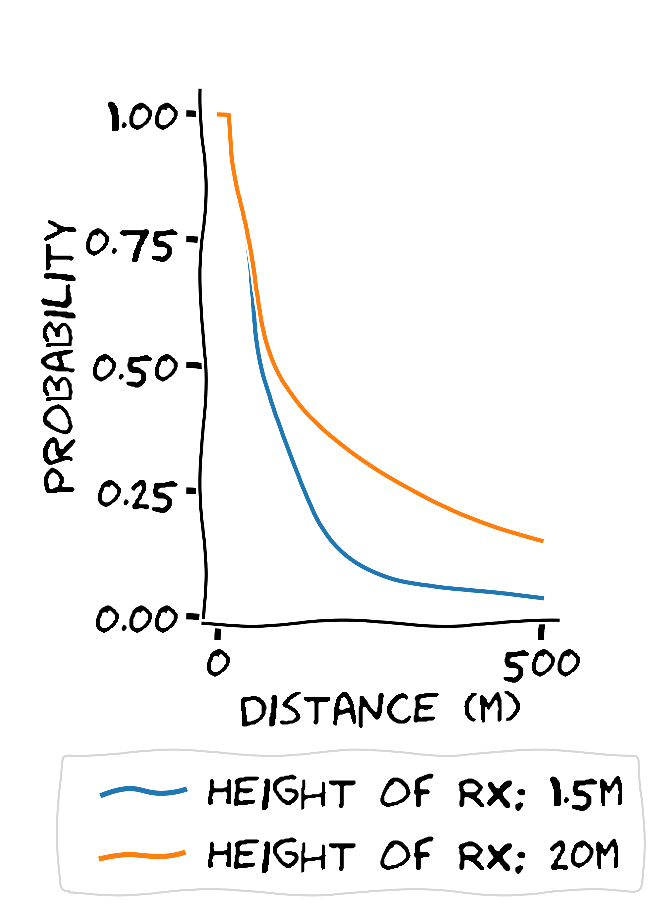
\includegraphics[]{chapters/part_pathloss/figures/LOS_probability.eps}
\caption{The probability of having line-of-sight for a given distance. Two scenarios of receiver height are shown. The probability of having \gls{los} within 25 meters is according to most models 1. }\label{fig:los_probability}
\end{marginfigure}



\subsection{Summary}

The features and details of the channel models described in 3GPP TR 38.901 and ITU-R M.2412 are extensive. Which is a definite need given the board range of supported frequencies (0-100 GHz). A brief view into the documents have been given in this section. It is found that both the documents contain empirical models for a series of different propagation scenarios. The empirical models are based on simple features that can be engineered without the need for complex geographical data. The empirical models are aided by stochastic methods for generating distributions of the most important impairments imposed by wireless transmission. Additionally the modelling approaches are fast and efficient making them useful for approximate predictions of path loss. Furthermore, both the documents contain useful guidelines for creating accurate stochastic channel models. 




\section{Ray-tracing}\label{sec:ray-tracing}

Ray-tracing models consider the physical presence of objects in the propagation model. Depending on the wavelength and the dielectric properties of the objects, the properties of the reflecting, diffracted or absorbed radio waves change. Ray-tracing is a useful tool for many applications, not only mobile communication systems, where the study of particles and their behaviour is to be studied. The recent advanced in computational resources (for instance by using \gls{gpu}) have enabled many advances in the area of ray-tracing technology.

In essence, ray-tracing is a propagation modelling tool that offers estimates, of not only path loss but also the angle of arrival, and the associated time delays. Computing these estimations is enabled by introducing the concept of \emph{rays} that have simplified properties of propagation compared to actual electromagnetic waves. This assumption has shown to be effective at approximating the essential characteristics of electromagnetic propagation. For instance, a ray travels in a straight line if the medium is homogeneous. Furthermore, it obeys the laws of refraction, reflection and diffraction and carries a set of energy \cite{Yun2015}. 
The principle of ray tracing is considering a single point source from which many rays are emanating, also termed \emph{ray-launching}, an example can be seen in Fig. \ref{fig:raytracing_launching}. The multitude of launched rays can then be grouped into different types depending on the interactions occurring in the propagation environment. Some rays are directly \acrlong{los} to the receiving point, causing them to be direct rays. Objects (depending on the material) reflect rays, and some are diffracted. Diffraction causes a single ray to produce a multitude of rays. The combination of these effects and the simplification of using the definition of \emph{rays} can effectively approximate the famous Maxwell equations.  Several algorithms for computing the behaviour of rays can be found in \cite{Yun2015} and references herein.


\begin{figure*}
    \centering
    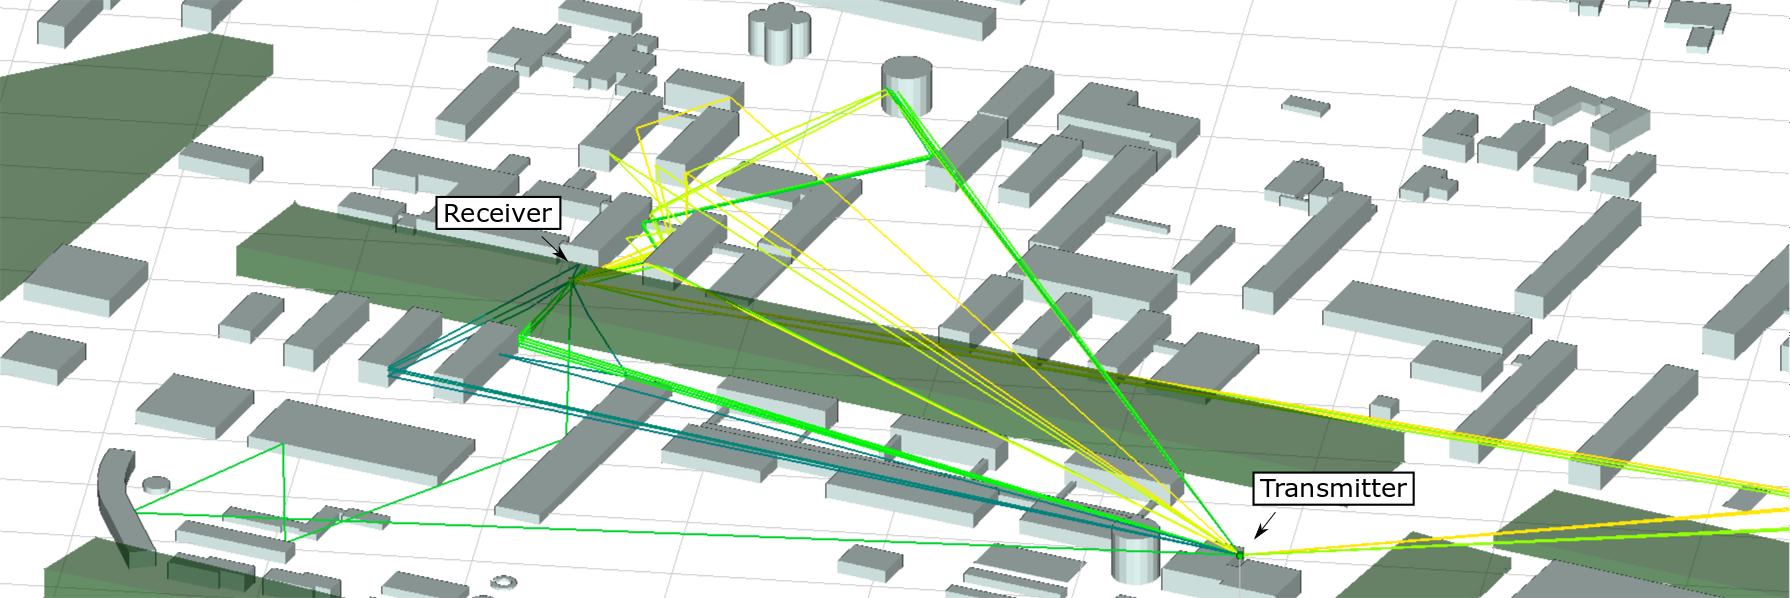
\includegraphics{chapters/part_pathloss/figures/RemcomRayLaunchingv2.png}
    \caption{An example of launched rays in Remcom Wireless Insite.}
    \label{fig:raytracing_launching}
\end{figure*}

In outdoor propagation scenarios of mobile communication systems the number of objects significantly vary from region to region. And furthermore, the number of relevant objects change significantly given the change in frequency and thus the wavelength. We use the term \emph{objects} here to represent any obstacle or \emph{thing} in the radio environment. This is for instance, buildings, vegetation, cars and even humans. By having detailed information on all objects in the propagation scenario ray-tracing solutions can be applied and the resulting propagation statistics of the \emph{rays} can be determined. However, it is also clear the such models are data exhaustive and increasingly so as the wavelength shortens \cite{Tse2005FundamentalsCommunication}. Thus for the multitude of high frequencies in the heterogeneous network architecture ray-tracing is simply unfeasible and challenging to approach. But, if the data is available the accuracy is in theory as close to the actual physical interactions as possible.

The data required for modern ray-tracing applied for use in mobile Communication systems can be split into several categories as below
\begin{itemize}
    \item Clutter (vegetation information)
    \begin{itemize}
        \item Position
        \item Height and type
    \end{itemize}
    \item Buildings
    \begin{itemize}
        \item Position
        \item Material composition
        \item Height and shape
    \end{itemize}
    \item Terrain
    \begin{itemize}
        \item Material composition
        \item Height
    \end{itemize}
\end{itemize}

The data only increases as a multitude of propagation scenarios are considered. For instance, in order to model \gls{o2i} propagation significant detail of not only the buildings and their material is required but also the internal layout and floor dimensions. In addition to these parameters, several configuration elements are also required. Such as the configuration of the transmitter and receiver antennas, along with calibrated noise figures representative of the hardware used. Modern ray-tracing engines such as Remcom Wireless Insite \cite{remcom} simplifies the procedure of integrating a large selection of data by having predefined material composition definitions with permittivity properties. However, not supplied by such modern engines is the data pipeline required for constructing the scene for modelling the propagation scenario. A contribution of this dissertation is the development of a $3$D ray-tracing model of Technical University of Denmark Campus. The necessary details and the resulting procedure for constructing such a model is outline for the remainder of this section.

\subsection{$3$D modelling}

The terrain information can in most cases be obtained using survey data, which is in most cases a necessary practice for many applications such as construction, utility and others. The Danish governmental institution \emph{styrelsen for dataforsyning og effektivisering} have made such data public and can be downloaded for free \cite{kortforsyningen}. Furthermore, the entire country of Denmark is \gls{lidar} scanned with high frequency (every 5-10 years) and high resolution. Such a public data set is paramount to obtaining the ray-tracing model as developed for this dissertation. More specifically \gls{lidar} data is supplied with a resolution of 4.5 measurements per $m^2$. An example of such data be seen in Fig. \ref{fig:lidar_data_example}. 

\begin{figure}
    \centering
    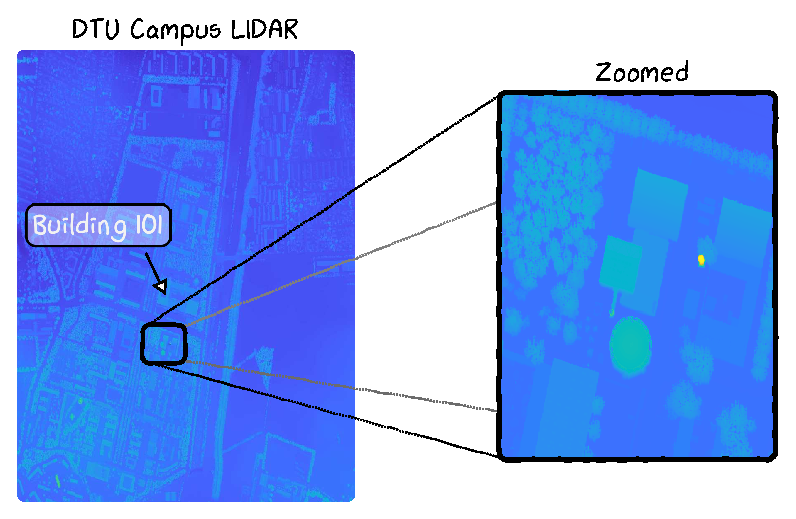
\includegraphics[width=\textwidth]{chapters/part_pathloss/figures/LIDAR_example.eps}
    \caption{Height measurements provided by \cite{kortforsyningen} using a LIDAR scan. Shown is DTU campus with a zoomed cutout. 4.5 points are available per $m^2$. Such data offer the basis for constructing a realistic 3D model for ray-tracing.}
    \label{fig:lidar_data_example}
\end{figure}

Even with this data, a significant effort is required to convert it to independent height of buildings. The procedure is three-fold. Firstly, it requires knowledge of building locations and their respective shapes. Secondly, assumptions of roofing and height must be applied for each building. Third, and lastly, the effective height of the buildings must be extracted. This was performed by utilizing the \gls{lidar} scans to effectively sample the height of buildings. The buildings were identified using zonal descriptions obtained through \gls{osm} \cite{OpenstreetMapWiki}. The mean of all samples within each building footprint (polygons) effectively provided an altitude measurement for each building, and thus a 3D polygon.

The exported file contains polygons, thus buildings and their shape with coordinates and the effective height of each polygon. The effective height is computed as the mean of $N$ number of \gls{lidar} measurements within the building footprints. Thus, if a roof is not flat a significant error to the building height is obtained. Thankfully, most buildings at DTU campus (if not all) have flat roofing. The file can be directly imported into Remcom Wireless Insite where further modelling of antennas are required. Additionally, and possibly even more import, is the definition of materials - this is where the model starts to become increasingly complex. A detailed description of the ray-tracing model can be found in Appendix \ref{app:ray_tracing_model}.

The authors in \cite{Vitucci2015} outline the difficulties of complex ray-tracing models, and more so, the resulting prediction accuracy. There exist a significant lack of literature comparing ray-tracing models and simple empirical models to experimental measurements. Even though the authors in \cite{Vitucci2015} argue the inaccuracy of ray-tracing models - it is still expected that a 3D model of the propagation scenario outperforms any empirical models due to the incorporation of propagation specific information. A result of such a study can be seen in the published work: \cite{Thrane2019ComparisonGHz}. The work compares the resulting 3D ray-tracing model with state-of-the-art empirical as detailed prior in this.



\section{Evaluation of classic methods}\label{sec:comparison_ghz_paper}
The result of a comparison study can be found in the published work \cite{Thrane2019ComparisonGHz}. Two operating frequencies are studied, specifically 811 MHz and 2630 MHz. The study compares existing methodologies such as ray-tracing (see section \ref{sec:ray-tracing}) and empirical models (see section \ref{sec:empirical_path_loss}) for predicting signal quality metrics of \gls{rsrp}. The study is based on experimental drive test data, more information can be found in Appendix \ref{app:drive_test_study_2017}. The measured \gls{rsrp} operates at a bandwidth of $20$ MHz. The base station location is kept constant, therefore the \gls{rsrp} is measured for a single base station with multiple sectors of different operating frequencies. 


\subsection{Results}

\begin{figure*}[thbp]
    \centering
    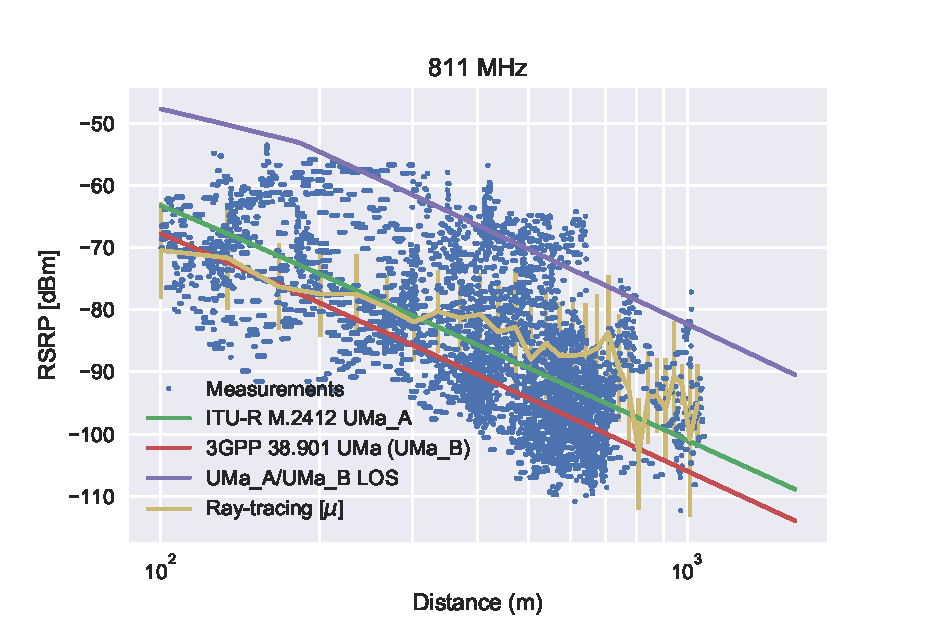
\includegraphics[width=0.48\textwidth]{chapters/part_pathloss/figures/results/811MHz_RSRP.eps}
    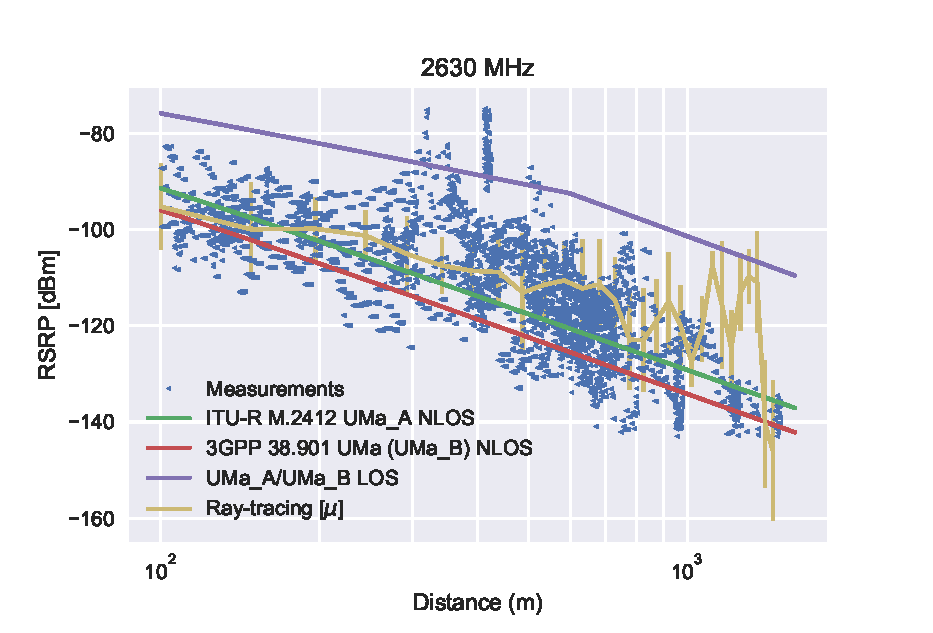
\includegraphics[width=0.48\textwidth]{chapters/part_pathloss/figures/results/2630MHz_RSRP.eps}
    % \vspace{1em}
    % \stepcounter{figure}\label{fig:rsrp_811_2630_distance}
    % \begin{flushleft}
    % \smallskip\noindent\footnotesize Figure \thefigure: The linear regression properties in the log-scale offered by 38.901 (thus \gls{uma}\_B) and ITU-R M.2412 (\gls{uma}\_A) for 811 and 2630 MHz. 
    % \end{flushleft}
    \caption{The linear regression properties in the log-scale offered by 38.901 (thus \gls{uma}\_B) and ITU-R M.2412 (\gls{uma}\_A) for 811 and 2630 MHz.}\label{fig:rsrp_811_2630_distance}
\end{figure*}

Measured \gls{rsrp} for 811 and 2630 MHz respectively can be seen in Fig. \ref{fig:rsrp_811_2630_distance}. The \gls{rsrp} predictions provided by both models, i.e. the ray-tracing and the empirical models are shown. The empirical models of \gls{3gpp} are utilized and termed \uma{B}. The empirical models provided by \gls{itu} M.2412 is denoted \uma{A}. Additional information can be found in section \ref{sec:empirical_path_loss}. The \gls{los} version of both empirical models are identical and shown for reference. 

The ray-tracing model offers point simulations. This is achieved by importing the drive test data into the ray-tracing environment. however, this results in no regression type comparative figure like the empirical models. The binned mean for each distance is shown for reference. A total of 30 bins are used for the averaging. The standard deviation is shown as errorbars. 

It can be seen from the results, that the binned average performance of the ray-tracing model is sufficient for lower distances. This can be seen by the average predicted \gls{rsrp} being more representative of the average \gls{rsrp} measured over the antenna distance separation. Additionally, a few \gls{los} clusters are observed which are well represented by the predictions of the empirical models. 



\begin{figure}
    \centering
    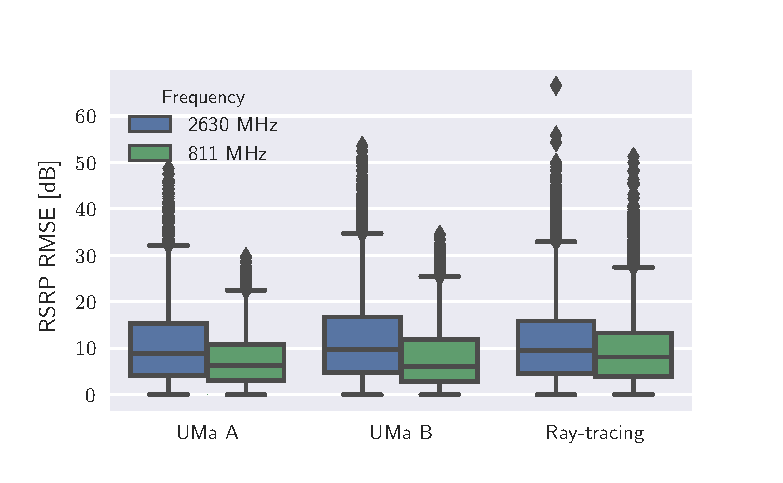
\includegraphics{chapters/part_pathloss/figures/results/improved_boxplot_results_comparison_ghz.eps}
    \caption{Predictive error of ray-tracing model for \gls{rsrp} at 811 and 2630 MHz compared to empirical models \uma{A} and \uma{B}.}
    \label{fig:rmse_boxplot_rsrp_comparison}
\end{figure}


The \gls{rmse} (See Eq. \ref{eq:rmse}) is used for evaluating the predictive performance of the empirical and ray-tracing methods. The results can be seen in Fig. \ref{fig:rmse_boxplot_rsrp_comparison}. The best performing model have the lowest \gls{rmse}. The best model is found to be \uma{A} with a \gls{rmse} of $7.6$ dB and $10.76$ dB at $811$ and $2630$ MHz respectively. The ray-tracing model is reported with an \gls{rmse} of $9.25$ dB and $11.13$ dB at $811$ and $2630$ MHz respectively. It can be observed that the performance of the \uma{A} model and the ray-tracing model at 2630 MHz is similar. Finally, it can be seen that on average an improvement in predictive performance of $\approx 3$ dB is achieved on $811$ MHz compared to that of $2630$ MHz.


% \begin{figure*}
%     \centering
%     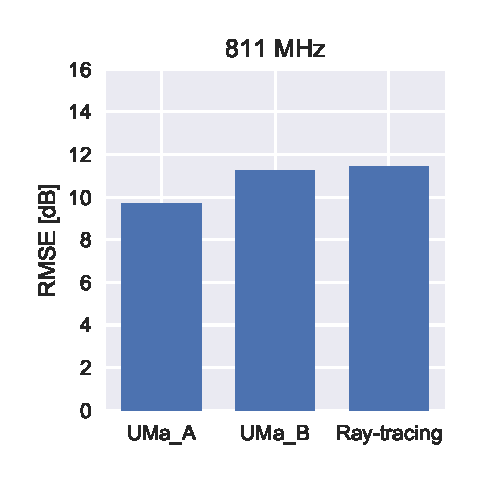
\includegraphics[width=0.48\textwidth]{chapters/part_pathloss/figures/results/811MHz_RMSE.eps}
%     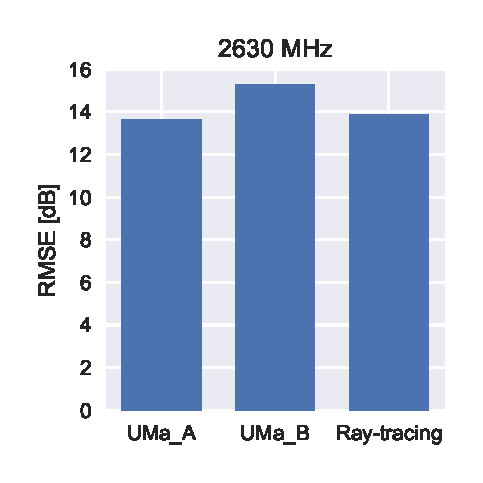
\includegraphics[width=0.48\textwidth]{chapters/part_pathloss/figures/results/2630MHz_RMSE.eps}
%     \vspace{1em}
%     \stepcounter{figure}
%     \begin{flushleft}
%     \smallskip\noindent\footnotesize Figure \thefigure: Error of the empirical path loss models and the ray-tracing model for 811 and 2630 MHz respectively.
%     \label{fig:rsrp_811_2630_RMSE}
%     \end{flushleft}
% \end{figure*}

\subsection{Discussion}
As indicated by the results, and as discussed in the paper \cite{Thrane2019ComparisonGHz}, the results are interesting for one primary reason. The ray-tracing model was expected to outperform the empirical models by some margin. This however, is not the case as the empirical \uma{A} model offers a predictive improvement in \gls{rmse} of $1.65$ dB at 811 MHz, and $0.37$ dB at 2630 MHz for \gls{rsrp}. This is contributed to several reasons, also found in existing literature \cite{Vitucci2015}. While the proposed ray-tracing model may seem complex the results show that it is not complex enough to accurately depict the realistic propagation setting of the measured area. This is identified to be caused by the following short-comings of the proposed ray-tracing model.

\begin{itemize}
    \item Clutter data in the ray-tracing model kept at a minimum.
    \item Approximation and generalization of building materials across architecture. 
    \item Concrete/brick materials assumed with a fixed and constant permittivity.
    \item Significant yearly difference between measurement study area and the LIDAR scan used for generating 3D objects.
    \item Inaccurate modelling of transmitting and receiving antennas
\end{itemize}

Additionally, the results show an overall decrease in predictive performance for all compared models at higher frequencies of $2630$ MHz. The results are inconclusive as to the reasons of this, but it is suspected that the increased frequency and thus lower wavelength increase the influence of smaller objects in the propagation scenario. These objects are not modeled by either the ray-tracing model or the empirical model.

\subsection{Conclusion}
The comparative study shows that current empirical path loss models for \gls{rsrp} predictions are capable of offering satisfactory performance in terms of $7.6$ dB and $10.76$ dB at $811$ and $2630$ MHz respectively. The measurements are furthermore compared to a ray-tracing model of the measured area. The initial hypothesis was that such a model would offer improved prediction performance compared to simple empirical models. This however is not the case, and a decrease in predictive performance is observed for a ray-tracing model, especially at $811$ MHz. Finally, it is found that predictions at $811$ MHz are on average $3$ dB improved to that at $2630$ MHz. 



\section{Summary}
This chapter have briefly introduced the area of wireless propagation modeling. Different models approaches have been introduced and the a comparative performance study have been presented and discussed. The scope of this chapter is reduced to \emph{empirical}- and \emph{ray-tracing}-based wireless channel models as they represent two inherently different means for computing the wireless channel propagation effects. An introduction to state-of-the-art empirical models as provided by \gls{3gpp} have been presented, along with an implementation of a ray-tracing model centered around the campus of the Technical University of Denmark. The differences between the models have been studied, both in terms of performance but also data complexity. The performance of both approaches were further studied by using measurements from a comprehensive drive test. The results showed that the ray-tracing models did not offer any performance gains compared to simple empirical models utilizing simple distance metrics. From theory it is clear that an increased amount of detail of the propagation area will result in more accurate computation of far-field statistics. However, this is not the case with the ray-tracing model implemented. Thus, in practice the increase of data complexity for wireless channel models does not directly translate to improvements in performance. 

While the proposed ray-tracing model suffer from large variability and poor performance several improvements have been identified. For instance, almost no clutter data is imported into the model and the model materials are very approximated. In any case, the empirical models have shown to offer satisfactory performance using simple metrics. Furthermore, the complexity of the model is highly dependent on the application needed. It is thus a constant trade-off between selecting the right model for the task at hand and the data available. Thus it is a challenge to model wireless propagation effects from not only the perspective of improved predictive performance, but also from a data complexity perspective. 

Not only is channel modelling a difficult task, it also impose practical problems of data engineering. It is of great interest to study how adaptive and iterative learned models perform on both performance accuracy but also computational performance. In the next chapter \gls{dl} for path loss estimation is introduced. While the task of current models consist of known model structures and methodologies, by applying \gls{dl} it is desired to learn the optimum model complexity through iterative learning principles as introduced in chapter \ref{ch:mlbasics}. The proposed methodology is shown to be effective in utilizing a completely data-driven approach of obtained measurements, but even more so, by introducing expert knowledge of path loss estimations (as introduced in this chapter) the stability and performance can be improved.
\chapter{Harnessing Meta-data}\label{ch:satelliteImages}
% \textcolor{red}{

% \begin{itemize}
%     \item What is the issue of current modelling methodologies?
%     \item \emph{Generalization} and \emph{Complexity}
%     \item How can Generalization be remedied? 
%     \item Obtaining features of propagation scenarios that are generalizable across propagation scenarios
%     \item how can Complexity be remedied?
%     \item 
    
% \end{itemize}}

Any kind of propagation modelling requires data of the propagation scenario. Detailing propagation-specific information requires data and a pipeline, regardless of propagation model. The necessary level of detail is directly related to the accuracy of the channel model. For instance, using principles such as ray-tracing the far-field statistics can be computed with high accuracy, but if and only if, the propagation scenario is described with sufficient detail. Accurate channel models consider a data complexity trade-off. By default, if more data is available, it will offer fewer generalization issues but in return, require a complicated data pipeline for modelling. Less data complexity results in more generalization issues. So, is there a sweet spot where the complexity is low, and the generalization is high? This chapter aims to explore this area and supply an attempt at answering such a question. The requirements for low and high complexity propagation modelling methods is outlined in Chapter \ref{ch:channelmodellingbasics} along with the basics of wireless channel propagation impairments. 


\section{Generalization and Complexity \label{sec:generalization}}



Generalization and complexity is the core issue of path loss prediction. If detailed propagation specific data can be obtained, one can obtain accurate path loss estimates using complex models such as ray-tracing. However, if such data is not available, simpler model using closed-form solutions with simple parameters are useful. It has been shown that both methodologies have their use cases. For instance, simpler path loss models are used for initial link budgets and preliminary studies, while more complex models are used for complex optimization and the research of novel solutions.


Simple path loss models are used in combinations with margins to ensure communication can be established. This however, will result in a margin of optimization and if channel models with higher accuracy could be utilized such a margin could be exploited. This exploitation could result in substantial gains in the overall cost of deployment and further optimization. So why not just use more accurate path loss models? They clearly exist and are well studied. In very simple terms, the data complexity is high and requires substantial efforts. In this chapter, \gls{dl} is applied to path loss estimation. More specifically, a novel \gls{dl} method is developed utilizing geographical images and expert knowledge for improving path loss estimation. Finally, the method is shown to be based on a feasible data complexity with a simplistic data pipeline that require no complex pre-processing procedures, such as required for ray-tracing models (See Section \ref{sec:ray-tracing}).

\subsection{Feature engineering}

Generalization has been a long standing issue for channel models as illustrated in \ref{sec:generalization}. In Machine Learning, the issue of generalization is also well studied and many direct comparisons can be made. It is well known, in the area of Machine Learning, that the features (and the resulting parameters of the model) are directly responsible for the performance on unseen data.  Such is the same in the area of channel models. Thus, it can be said that the performance of channel models are directly related to the input parameters used, or in other words, the features used. A comprehensive study of input parameters (features) and the relation to path loss can be found in \cite{Popoola2019}. 
 
Examples of features used in combination with \gls{nn}: \emph{Longitude, Latitude, Distance, elevation, Altitude, Clutter height, portion through building, height, thickness, transmitting power, street width, building height, building speration, transmitter position, street orientation, base station antenna and rooftop height difference, direct ray, reflected ray from ground, two dominant reflected rays, frequency}

The primary difference between models such as empirical models (See Eq. \ref{eq:uma_nlos_pathloss_max}), and \gls{nn}-based models can be outlined in simple terms. In Machine Learning, the aim is not only to discover the best parameters, e.g. features, but also the best model. Traditional path loss models are the result of significant research and measurement campaigns. Therefor, the path loss models is the result of a curve-fit given parameters that have statistical importance to the path loss. In such cases, the model is known and takes a from that is similar to that of Eq. \ref{eq:pathloss_model} (but with additional terms to account for various attenuation differences).

The features used in \gls{nn}-based models versus traditional path loss models are similar for good reason. Having a complete data-driven approach should ultimately provide with similar answers as research have provided in terms of traditional path loss models. The benefit of working with adaptive models is that statistical knowledge is not necessary and is inferred from obtain observations. For instance, by using adaptive models, features that are not directly related to path loss (or at least by some unknown factor) are used to improve predictive performance. This have benefits and downsides. The benefits are that the performance of the models will improve as more data is obtained. The downside is that the performance can be challenging to evaluate with respect to propagation scenarios inherently different from where measurements have been obtained. With that being said, the end goal of path loss models must be to offer generalization regardless of propagation scenario and the features used. This goal is identical whether a traditional single-slope path loss model is used, or it is the product of training. 

Ultimately \gls{nn} are limited in performance by the engineered features \cite{Alom2019AArchitectures}. Meaning, while the use of traditional \gls{nn} approaches may yield significant improvements to empirical models they are limited by the engineered features. This is not the case for \gls{dl}-based models. such models seek to learn from raw data. In this case we look towards the use of geographical images for improving the estimation of attenuation caused by large-scale parameters.


\section{Use of satellite imagery}

To avoid the need for complicated features, and time-consuming feature engineering aspects, we look towards \gls{dl}. The main principles of \gls{dl} and subsequently \gls{ml} are highlighted in Chapter \ref{ch:mlbasics}. 

A novel methodology for path loss and signal quality parameter approximation using satellite images is proposed in this thesis. The results of the documented methods have resulted in three publications \cite{Thrane2018DriveApproximation, Thrane020ModelAidedDeepLearning, Thrane2020DeepKnowledge}. The main contributions of the publications are introduced in the remainder of this chapter, along with a more in depth discussion and conclusion. The model architecture for providing path loss and received signal quality metrics using satellite images have been under constant evolution. A significant difference in model architecture and complexity can be observed for all proposed methods.  For cohesion, all methods and the resulting performance is outlined in this section. However, all methods share the same essential component, utilizing images for improving signal quality parameter prediction. The evolution of the proposed method can be termed according to the iterations, thus \cite{Thrane2018DriveApproximation} as \emph{version 1 (v1)}, \cite{Thrane020ModelAidedDeepLearning} as \emph{version 2 (v2)} and \cite{Thrane2020DeepKnowledge} as \emph{version 3 (v3)}. 
\begin{itemize}
    \item A summary of \emph{version 1} can be found in Section \ref{sec:summary_version1}. 
    \item A summary of \emph{version 2} can be found in Section \ref{subsec:conclusion_v2}. 
    \item A summary of \emph{version 3} can be found in Section \ref{subsec:conclusion_v3}
    \item Discussion, Conclusion and future outlook can be found in Section \ref{sec:satellite_image_discussion}
\end{itemize}
\noindent
High resolution satellite images of areas are obtainable using such services as the \emph{static API} from Google Maps \cite{GoogleAPI}, or Mapbox API \cite{MapboxWebsite}. The latter is utilized for this work. The idea of predicting path loss from such images stems mainly from the data availability, but also because such images outline the actual details of a propagation environment. The magnitude of details present in high resolution satellite images greatly surpass that of available open-source meta-data used in models such as ray-tracing. In order to formalize the use of satellite images for path loss prediction, several factors and features needs to be considered in order to aid the learning process. Given the empirical knowledge of path loss in outdoor propagation scenarios as presented in Chapter \ref{ch:channelmodellingbasics}, we can hypothesise where such images may offer the most gain. Local variability, is a term describing losses associated with local obstacles in relation to a receiver position for instance, buildings or vegetation. The primary purpose of the satellite images is to assist in determining attenuation related to local variability from imagery that visualize the local area of the receiver. Thus, in order to effectively utilize such images, they must contain information of local variability, e.g. the large-scale fading present in the environment. In order to do so the images must be of high enough resolution such that buildings, vegetation and other structure can clearly be observed.


\subsection{Problem statement}

The function we desire to learn is the received power for a given position in relation to the transmitter. If the reader recall the link-budget from \ref{ch:channelmodellingbasics}. It takes the form
\begin{equation}
    P_{rx} = P_{tx} + G_{tx} + G_{rx} + L_{rx} + L_{tx} + \underbrace{L(x,y)}_{\text{Path loss}}
\end{equation}
The received power is dependent thus on constants, such as transmission power, gains associated with the transmitter and receiver and losses hereof. The mostly unknown constant of the link budget is dependent on the position in the radio environment. Thus the function we desire to learn consists of constants, and a function that is positional dependent.  

The task is to obtain a model that can continuously predict received power given an image and some position location features. In the world of \gls{ml}, such a model is of type \emph{regression} and follows the form:
\begin{equation}\label{eq:dl_model_satellite}
    t_n = y(x_n, \mathbf{w}, \theta) + \epsilon
\end{equation}

Where $y(\cdot)$ is the function we desire to learn given input parameters $x_n$, a set of learned weights $\mathbf{w}$ and some hyper-parameters $\theta$. We define the output of the model $t_n$. Different techniques can be used to learn the function $y(\cdot)$, in this work \gls{dnn} are used due to the use of images. The methodologies associated with vision type models are rooted in \gls{nn}-based models.



We define the a single input to consists of the following

\begin{equation}\label{eq:dnn_inputs}
    x_n = [\text{lat}, \text{lon}, B_{tx}, d_{\text{lat}}, d_{\text{lon}}, d, \mathbf{A}]
\end{equation}

$\text{lat}, \text{lon}$ identify the geographical coordinates of the receiver, $B_{tx}$ is a variable used to identify the transmitter. $ d_{\text{lat}}, d_{\text{lon}} $ denote the distance in latitude and longitude direction respectively. $d$ denote the distance straight as the crow flies. It is important to note that the only engineered features are the distance metrics, as they are derived based on position of the receiver and the transmitter. $\mathbf{A}$ is used to denote the image of the local area around the receiver position. 

In order to be able to capture and process images, principles from computer vision are applied. This is termed \gls{cnn} as described in Section \ref{sec:convolutions} and uses convolution operations to process the properties of images.

This is posed as a supervised learning problem, thus for each system input ($x_n$) a target is required ($t_n$). The LTE-A reference parameter \gls{rsrp} is used as a definite approximation of received power for the transmitting base station. \textcolor{red}{Define RSRP}. Thus $t_n = \text{\gls{rsrp}}$. It should be noted that several targets can be assigned for the same input, as accomplished in \cite{Thrane2018DriveApproximation}, such as \gls{rssi} and \gls{sinr}. The reason for not including these in later research are described in Section \ref{sec:satellite_image_discussion}.

To learn in a supervised fashion, a cost function is required. The sum-of-squares error function between the model output and the observation is used Eq. (\ref{eq:sum-of-squares}). If recalled, minimizing such an error function corresponds to maximize the likelihood function if the targets have noise that is Gaussian distributed. This is also denoted as $\epsilon \sim \mathcal{N}(\mu,\,\sigma^{2})$ from Eq. (\ref{eq:dl_model_satellite}). If the reader can recall from Chapter \ref{ch:channelmodellingbasics}, the distribution of local variability, e.g. large-scale fading can be approximated with a log-normal distribution. We thus assume, that the observations of $t_n$ are under the influence of large-scale fading.

The optimization is complete using principles of gradient descent and back propagation, as detailed in Section \ref{sec:neural_networks}.



\subsection{Images}


\begin{figure}[h]
    \centering
    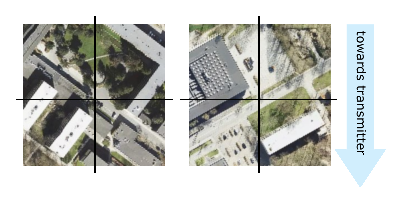
\includegraphics{chapters/part_pathloss/figures/satellite_example.eps}
    \caption{Example of satellite images and the proposed rotation to separate transmitters in same locations.}
    \label{fig:satellite_example}
\end{figure}
A single image of size $256 \times 256 \times 3$ (width, height, RGB color channels) was obtained for each measurement. The area spanned by the images corresponds to roughly $180 m^2$. The reasoning for the image size and the area covered was mainly sparked from the observed level of detail. The images contain a large enough area to display important buildings and vegetation with sufficient detail. When constructing the dataset with the images, two main concerns arose
\begin{enumerate}

    \item Measurements from different transmitters at the same position, how would the images need to differ?
    \item How to embed distance between transmitter and receiver?
\end{enumerate}

The approach for 1) was to rotate according to the transmitter. That way, images are the same area (or same position even) were inherently different. A fixed image size is simplifies the \gls{dl} model greatly, so it was avoided to embed further information into the images. to ensure 2) is addressed, the distance was thus given as a feature along with the positional locators. This ensure the primary objective of the images, is to offer information of geostatistics representing local variablility. An example of such a rotation can be seen in Fig. \ref{fig:satellite_example}.



\section{Signal quality prediction utilizing Satellite images (v1)}\label{sec:initial_v1}
The system documented in \cite{Thrane2018DriveApproximation} explores the use of colourized satellite images and multiple signal quality metrics as output, e.g. \emph{v1}. The inputs are separated into two neural networks and at a later stage combined into a deep output layer. The inputs and outputs can be observed in Fig. \ref{fig:dnn_architecture_drive_test_minimization}. For this work, the approach was to develop a method that can minimize drive testing, as this is an expensive practice as also highlighted in section \ref{sec:drive_testing}.

\begin{figure}
    \centering
    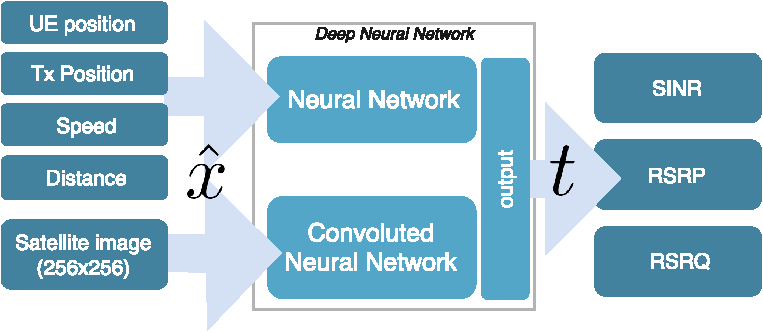
\includegraphics{chapters/part_pathloss/drive_test_minimzation_paper/input_output_figure.pdf}
    \caption{Model architecture used in \cite{Thrane2018DriveApproximation} with a multiple of outputs. Two neural networks are used and concatenated at the output layers.}
    \label{fig:dnn_architecture_drive_test_minimization}
\end{figure}

The size of the layers for both the convolutional neural network and the regular neural network can be seen in Table. \ref{tab:dnn_architecture_drive_test_minimization}

\begin{table}[ht]
  \centering
  \caption{Architecture and layer size of the model used in \cite{Thrane2018DriveApproximation}.}
  \label{tab:dnn_architecture_drive_test_minimization}
  \begin{tabular}{l|l|l}
                & NN settings     & CNN settings      \\ \hline
  Layer size & $[40, 40]$      & $[32, 16, 16, 8]$ \\
  Dropout       & $0.3$           & $0.1$             \\
  Activation    & \textit{ReLU} & \textit{ReLU}  
\end{tabular}
\end{table}

The only regularization added to the model weights were done using dropout layers. The use of dropout layers further enabled so-called \emph{Bayesian approximation} through Monte-Carlo sampling of the layers. The principles are explained in Section \ref{sec:neural_networks}. 

The drive tests detailed in Appendix \ref{app:drive_test_study_2017} compromised the foundation for the data set used for training. The measurements were split into more defined routes as to \emph{emulate} the process of a drive-test and thus limit the available amount of training examples. A total of $39000$ input and target pairs constructed the data set. Of the $\sim 39000$, $\sim 9000$ compromised the test set, as also shown in blue in Fig. \ref{fig:drive_test_routes_split}. Two specified routes, \texttt{Route 1} and \texttt{Route 2}, compose the testing set. Colourized images were used as input to the Deep Learning model. The images were downloaded from Mapbox API \cite{MapboxWebsite}. The colourized images were rotated according to the transmitter to distinguish images at the same position but from different transmitters.

\begin{figure}
    \centering
    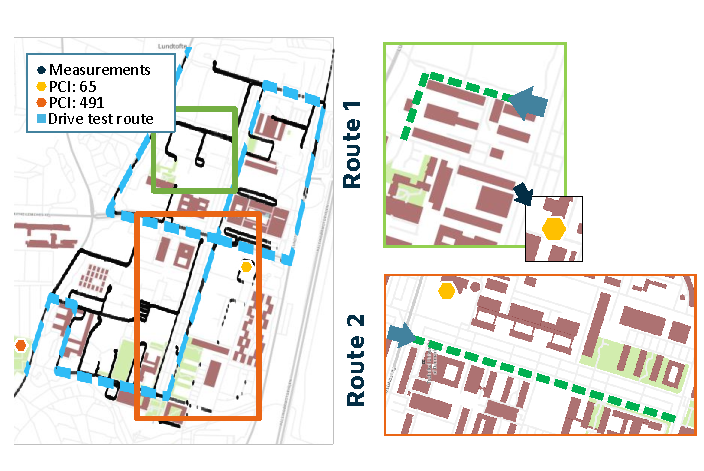
\includegraphics{chapters/part_pathloss/drive_test_minimzation_paper/route_drawing.pdf}
    \caption{The majority of roads at DTU campus area were covered during drive testing. The training was isolated to the main roads of campus, while two specific routes were isolated for testing and evaluation, \texttt{Route 1} and \texttt{Route 2}.}
    \label{fig:drive_test_routes_split}
\end{figure}

The implementation and training of the model was done with open-source libraries \emph{Keras} \cite{chollet2015keras} with \emph{TensorFlow} \cite{tensorflow2015-whitepaper}. The training was accelerated with GPU and mini-batch training. The batch size was heavily limited by the RAM available on the GPU device and was thus limited to $5$. 


\subsection{Results}
\begin{marginfigure}
    \centering
    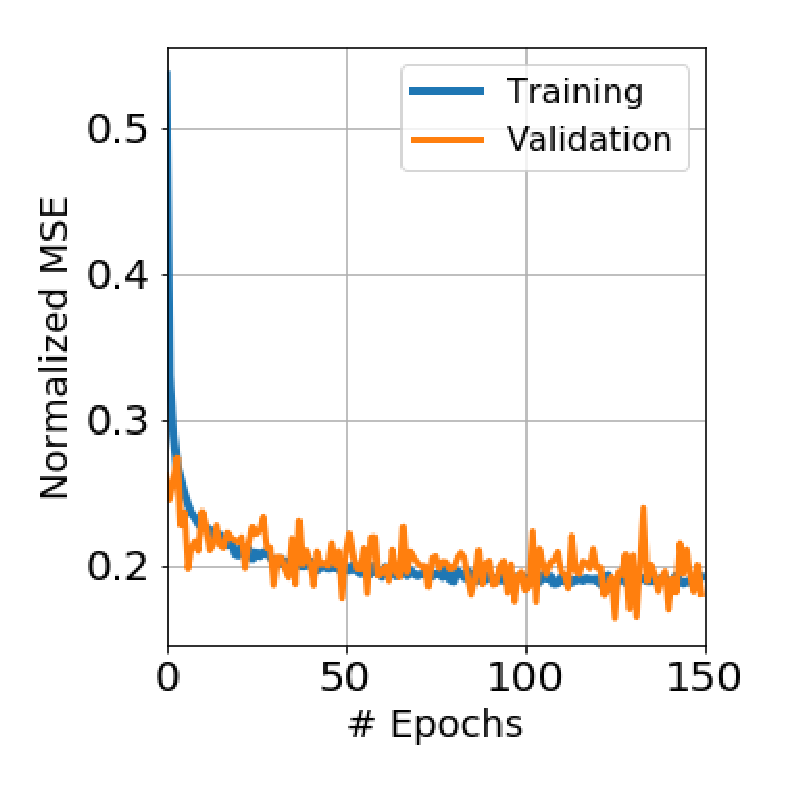
\includegraphics{chapters/part_pathloss/drive_test_minimzation_paper/training_val_test_5ab7fb562d60543b24f857af.eps}
    \caption{Training and validation error for the training of the model.}
    \label{fig:training_val_error}
\end{marginfigure}

The \gls{rmse} error for both rest routes can be observed in Table \ref{tab:rmse_error_v1} for all output metrics. The sampled standard deviation $\sigma$ using the Bayesian approximation method is also presented. The standard deviation can also be presented in terms of a confidence interval, as visualized in Fig. \ref{fig:route_1_v1} (RSRQ as a function of measurement) and \ref{fig:route_2_v1} (RSRP as a function of measurement) along with the prediction (the mean $\mu$) for both rest routes. The measurements are sorted sequentially so the route progression can be studied. This allows for the evaluation of the obstacles during the measurement sequence. For instance, a large obstacle (building) is observed in the radio environment and can be identified by the prediction of the model. 

The \gls{rsrp}, as a function of measurements for route 2, is shown in Fig. \ref{fig:route_2_v1}. It can be seen that a significant decrease in \gls{rsrp} is observed for both predictions and measurements. The decrease in \gls{rsrp} is due to the sequence of measurements. The sequence is increased separation between the transmitter and the receiver, i.e. the vehicle moving away from the \gls{enb}. The trained model captures this and provide sufficient predictions of \gls{rsrp} with an added confidence interval. Most of the measurements are within the $95\%$ confidence interval, which illustrates the usefulness of the Bayesian approximation. 

The training and validation error is shown in Fig. \ref{fig:training_val_error}. The final test error performance of the system (in terms of normalized MSE) was observed to be $\mathbf{0.37}$ MSE. 

\def\arraystretch{1.5}
\begin{table}[]
\centering
\begin{tabular}{@{}lll@{}}
\toprule
\textbf{Parameter} & RMSE   & $\pm \sigma$ \\ \midrule
SINR               & $5.2$ dB & $4.1$ dB       \\
RSRP               & $7.7$ dB & $5.9$ dB       \\
RSRQ               & $3.1$ dB & $2.2$ dB       \\ \bottomrule
\end{tabular}
\caption{\gls{rmse} for both rest routes with the sampled $\sigma$ }\label{tab:rmse_error_v1}
\end{table}



\begin{figure}
    \centering
    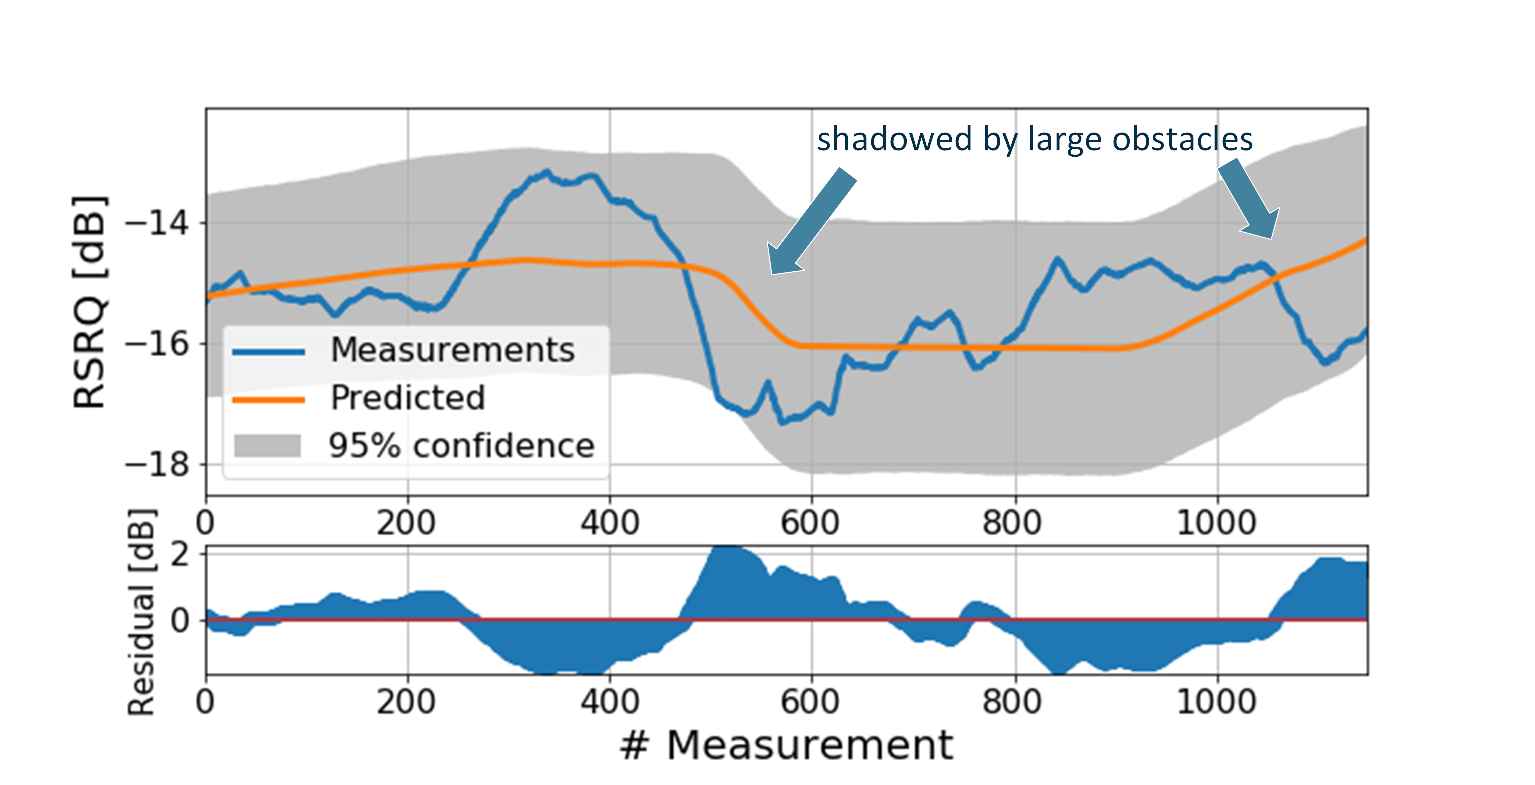
\includegraphics{chapters/part_pathloss/drive_test_minimzation_paper/route_1_predictions_5ab708662d60543b24f857a1_annotated.eps}
    \caption{Prediction of \texttt{route 1} \gls{rsrq} with added $95\%$ confidence interval.}
    \label{fig:route_1_v1}
\end{figure}


\begin{figure}
    \centering
    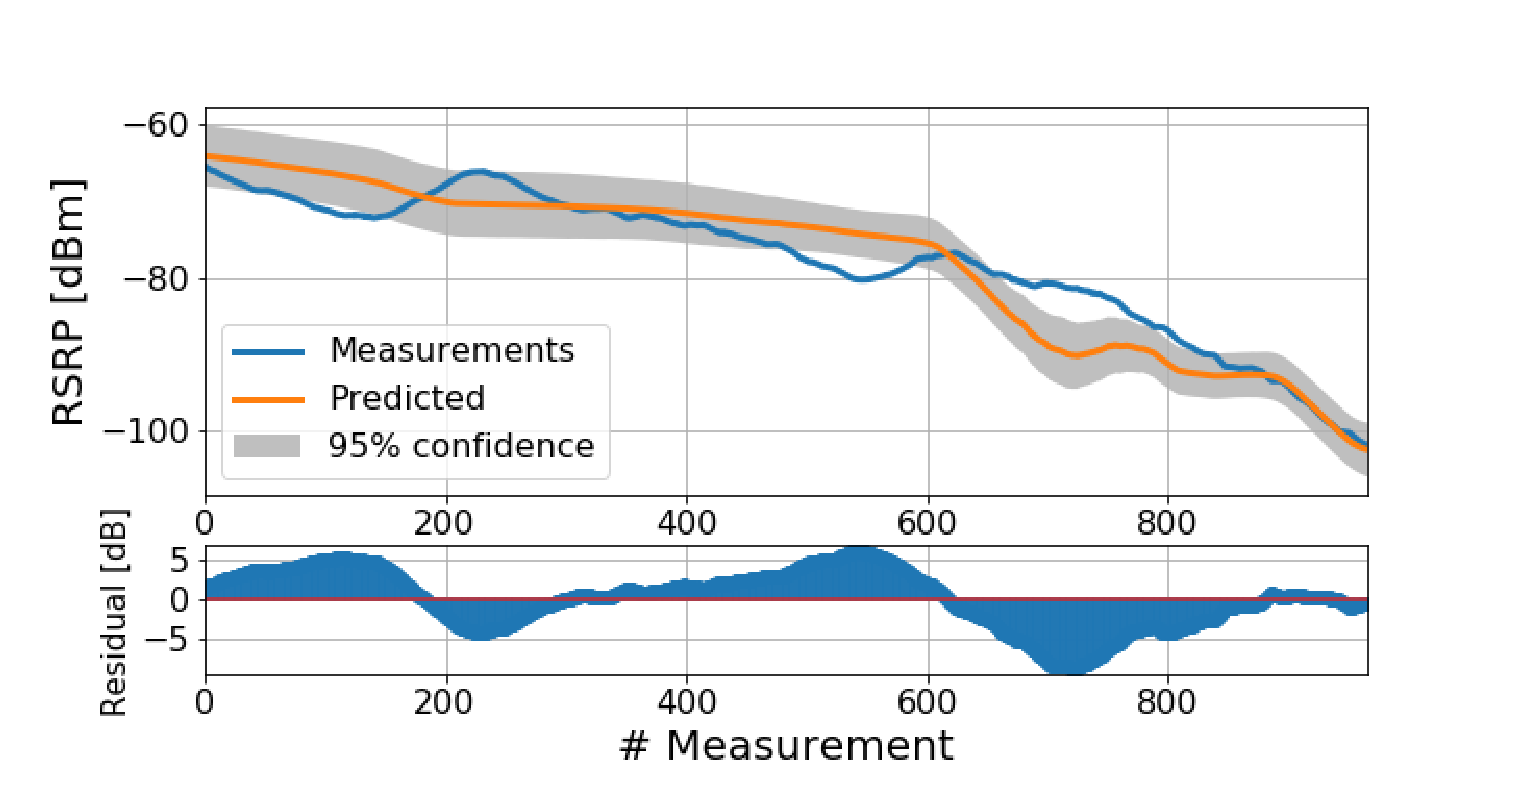
\includegraphics{chapters/part_pathloss/drive_test_minimzation_paper/route_2_predictions_5ab708662d60543b24f857a1.eps}
    \caption{Prediction of \texttt{route 2} \gls{rsrp} with added $95\%$ confidence interval.}
    \label{fig:route_2_v1}
\end{figure}

\subsection{Discussion and Conclusion}
It has been shown that the trained model is capable of providing accurate predictions in unseen areas using limited training data. This was evaluated using two independent routes for testing, e.g. \texttt{route 1} and \texttt{route 2}. From the prediction results of \texttt{route 1}, it was observed that the model is capable of achieving some insight into the local variability. However, it is unknown if the images or sufficient information causes this insight through distance features. It does indicate that the satellite images are useful; however, it requires further studies. 
For \texttt{route 2}, the model is observed to be capable of providing a decrease in \gls{rsrp}, which is primarily related to transmitter and receiver separation distance. 

In terms of model generalization, some issues exist. This is highlighted by the gap between training/validation and test error; thus, further model regularization can improve the overall prediction accuracy of the system. In summary, the \emph{version 1} of utilizing satellite images provided the following conclusion

\begin{itemize}
    \item The model is capable of predicting a drop in \gls{rsrq} explained by the shadowing of a large building.
    \item The model is capable of predicting an accurate decrease in \gls{rsrp} as a function of transmitter-receiver antenna separation.
    \item The gap between training and test error highlights generalization issues
\end{itemize}

It is thus of interest to explore 1) the specific prediction improvements caused by images and 2) the generalization of the model (and techniques hereof).

\section{Generalization issues}\label{sec:summary_version1}
The method has some shortcomings, especially related to generalization. The gap between the test and training set is seen as being significant. However, and possibly most interesting, the documented work introduces the novel idea of introducing automatized meta-data extraction for use in path loss estimation.
As recalled by section \ref{sec:generalization}, \glspl{nn} are capable of providing a satisfactory regression solution to path loss prediction. It is possible and likely that the majority of the accurate path loss predictions are directly related to the primary feature \emph{distance}. The results show that some large-scale fading impairments can be predicted; however, it is unknown if this is due to image-related features. Further studies were deemed a necessity. Specifically, a benchmarking study against traditional path loss prediction methodologies would identify and quantify both the shortcomings and benefits of the documented method. Additionally, it is of interest to study the specific performance gain offered by the inclusion of images. Such a study was completed and published in \cite{Thrane020ModelAidedDeepLearning}.  

\section{Embedding expert knowledge (v2)}\label{sec:expert_v2}
The architecture of the method was completely revised for the second study to ensure the possibility of validating and studying two particular aspects that are of interest:

\begin{itemize}
    \item Generalization improvements by aided learning (expert knowledge)
    \item Performance improvements by images
\end{itemize}

Obtaining generalization in any \gls{ml}-type solutions remains the primary objective of any engineered \gls{ml} solution. Recently, papers introducing model-aided learning have gained popularity due to the achieved generalization properties and the overall simplification in the learning process. It is argued that scientists over the recent decades have constructed quite good models for the reality we live in, and such models should be utilized in \gls{ml} processes. 

What sparked the idea and interest was the work detailed in \cite{Zheng2016}, where a robot is tasked with throwing and catching objects. To throw and catch objects accurately, a predictive model is necessary. The authors show that by utilizing a basic ballistic model for predicting the trajectory in combination with a \gls{ml} system, significant performance gains can be achieved. More specifically, considerable accuracy improvements could be gained by introducing a simple model into the learning process. Even though the model is not accurate, it assisted the learning process to learn the unknown factors associated with the overall throwing system, for instance, the complexity added by the friction of the mechanical joints in the robot etc. This approach reduced the whole learning task from learning the entirety of the system, including the ballistic model, to only learn a correction of the theoretical ballistic model.

Aiding the \gls{ml} models with expert knowledge have been shown to be useful for path loss estimation in \cite{Cavalcanti2017} while expert knowledge for utilization in wireless systems has been hailed as a necessity for future \gls{ml}-based and \gls{dl}-based solutions \cite{Zappone2019}.

Given the recent results of \cite{Thrane2019ComparisonGHz} also seen in section \ref{sec:comparison_ghz_paper}, simple empirical path loss models were evaluated to be valuable. The second version was thus the integration of simple empirical models into the path loss prediction to improve the shortcomings identified in \emph{version 1}. 

\begin{figure*}
    \centering
    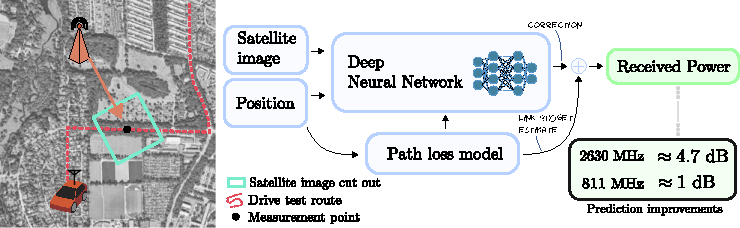
\includegraphics{chapters/part_pathloss/model_aided_paper/version2_approach_figure.pdf}
    \caption{The improved approach introduces expert knowledge for improving training stability and testing accuracy.}
    \label{fig:my_label}
\end{figure*}

\subsection{Model architecture}
The model definition was changed and simplified to adjust to isolated experiments. The previous model architecture provided several output metrics of signal quality, in order to determine the performance increase of the model approach this was isolated to a single output parameter, namely \gls{rsrp}. I.e. we define the model as:

\begin{equation}\label{eq:model}
    y(x_n, \mathbf{w}, \bm{\theta}) = \underbrace{z([x_n, L(d)], \mathbf{w}, \bm{\theta})}_{Correction} + L(d)
\end{equation}

Where $z(\cdot)$ is the model of the \gls{dnn}. The $L(d)$ term is an integrated path loss model and provides an estimated link budget. The link budget is estimated as:

\begin{equation}\label{eq:path_loss_model_linkbudget}
L(d) = PL(d) + G_{tx} + L
\end{equation}

Where $PL(d)$ is the \uma{A} path loss model as detailed in Chapter \ref{ch:channelmodellingbasics}. $G_{tx}$ is the estimated transmission power and related gains (constant). We define $L$ as additional losses, such as cable loss and antenna attenuation (constant). 

The defined model is still formalized concerning regression, e.g. Eq. (\ref{eq:dl_model_satellite}) is still the case, however $t_n = RSRP$ and not a vector including such output metrics of \gls{rsrq} etc. The path loss model is integrated into the supervised learning process, as shown in Fig. \ref{fig:combined_model_approach}. The task of the \gls{dnn} is no longer to learn and approximate the received power by itself, it is aided by expert knowledge: a simplified path loss model. We term the output of the \gls{dnn} a \emph{correction}.


\begin{figure}
    \centering
    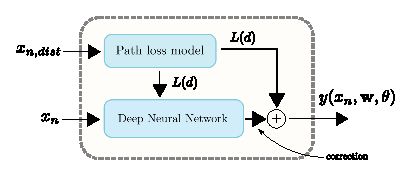
\includegraphics[width=\textwidth]{chapters/part_pathloss/model_aided_paper/combined_model_approach.eps}
    \caption{Combining a path loss model and a \gls{dnn} for estimating \gls{rsrp}.}
    \label{fig:combined_model_approach}
\end{figure}

 $x_{n,dist}$ defines the 3D distance for each measurement point, which, is provided as a feature to the \gls{dnn}. The list of features is the same as presented in Eq. (\ref{eq:dnn_inputs}) with one exception. The estimated link budget is added to the list and is further visualized in Fig. \ref{fig:satellite_model_setup_v2}.
 
The \gls{dnn}, as seen in Fig. \ref{fig:satellite_model_setup_v2} utilize two fully-connected neural networks, and a convolutional neural network. The \gls{nn} termed \texttt{NN} is tasked with managing the engineered features, while the \gls{cnn} is tasked with processing the satellite images. The output of both \gls{nn} are added and combined into a \gls{nn} termed \texttt{NN2}, tasked with processing the information provided by the engineered features and the satellite images resulting in a single output metric. The size of the layers can be seen in Table \ref{tab:cnn_structure} and \ref{tab:nn_structure}.

\begin{figure}
    \centering
    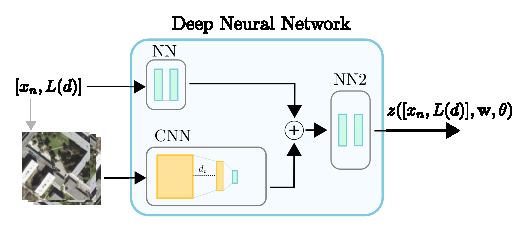
\includegraphics{chapters/part_pathloss/model_aided_paper/setup_model.eps}
    \caption{The Deep Neural Network consists of a convolutional neural network (\emph{CNN}) and two fully connected neural networks, \emph{NN} and \emph{NN2}.}
    \label{fig:satellite_model_setup_v2}
\end{figure}

\subsection{Training}\label{sec:training_v2}
The training of the model was accomplished using Pytorch \cite{Paszke2017AutomaticPyTorch}. The training makes use of backpropagation and the minimization of \gls{mse} loss as described in chapter \ref{ch:mlbasics}. Additionally, the findings of \emph{system v1} highlight the requirement for further generalization techniques. Data augmentation of the images is a common practice to improve dataset size and reduce overfitting during training \cite{Shorten2019ALearning}. The purpose is to feed the algorithm slightly different versions of the same image as to explore the generalization of the method. This was achieved by using a \emph{random  affine  transformation} that shears and rotate the image random but keeps the center of the image invariant. Examples of the data augmentation can be seen in Fig. \ref{fig:data_augmentation}. The transformation utilizes a random rotation angle of $\pm 20$ degrees with $\pm 10$ degrees of shear. The augmentation if applied to the original images for every observation, e.g. for every training iteration. In other words, the original images supplied are randomly transformed during each training iteration. A large finite number of versions of the original image are produced, effectively increasing the amount of available images. Unlike \emph{v1}, grey-scaled images were used to improve generalization. 


\begin{figure}
    \centering
    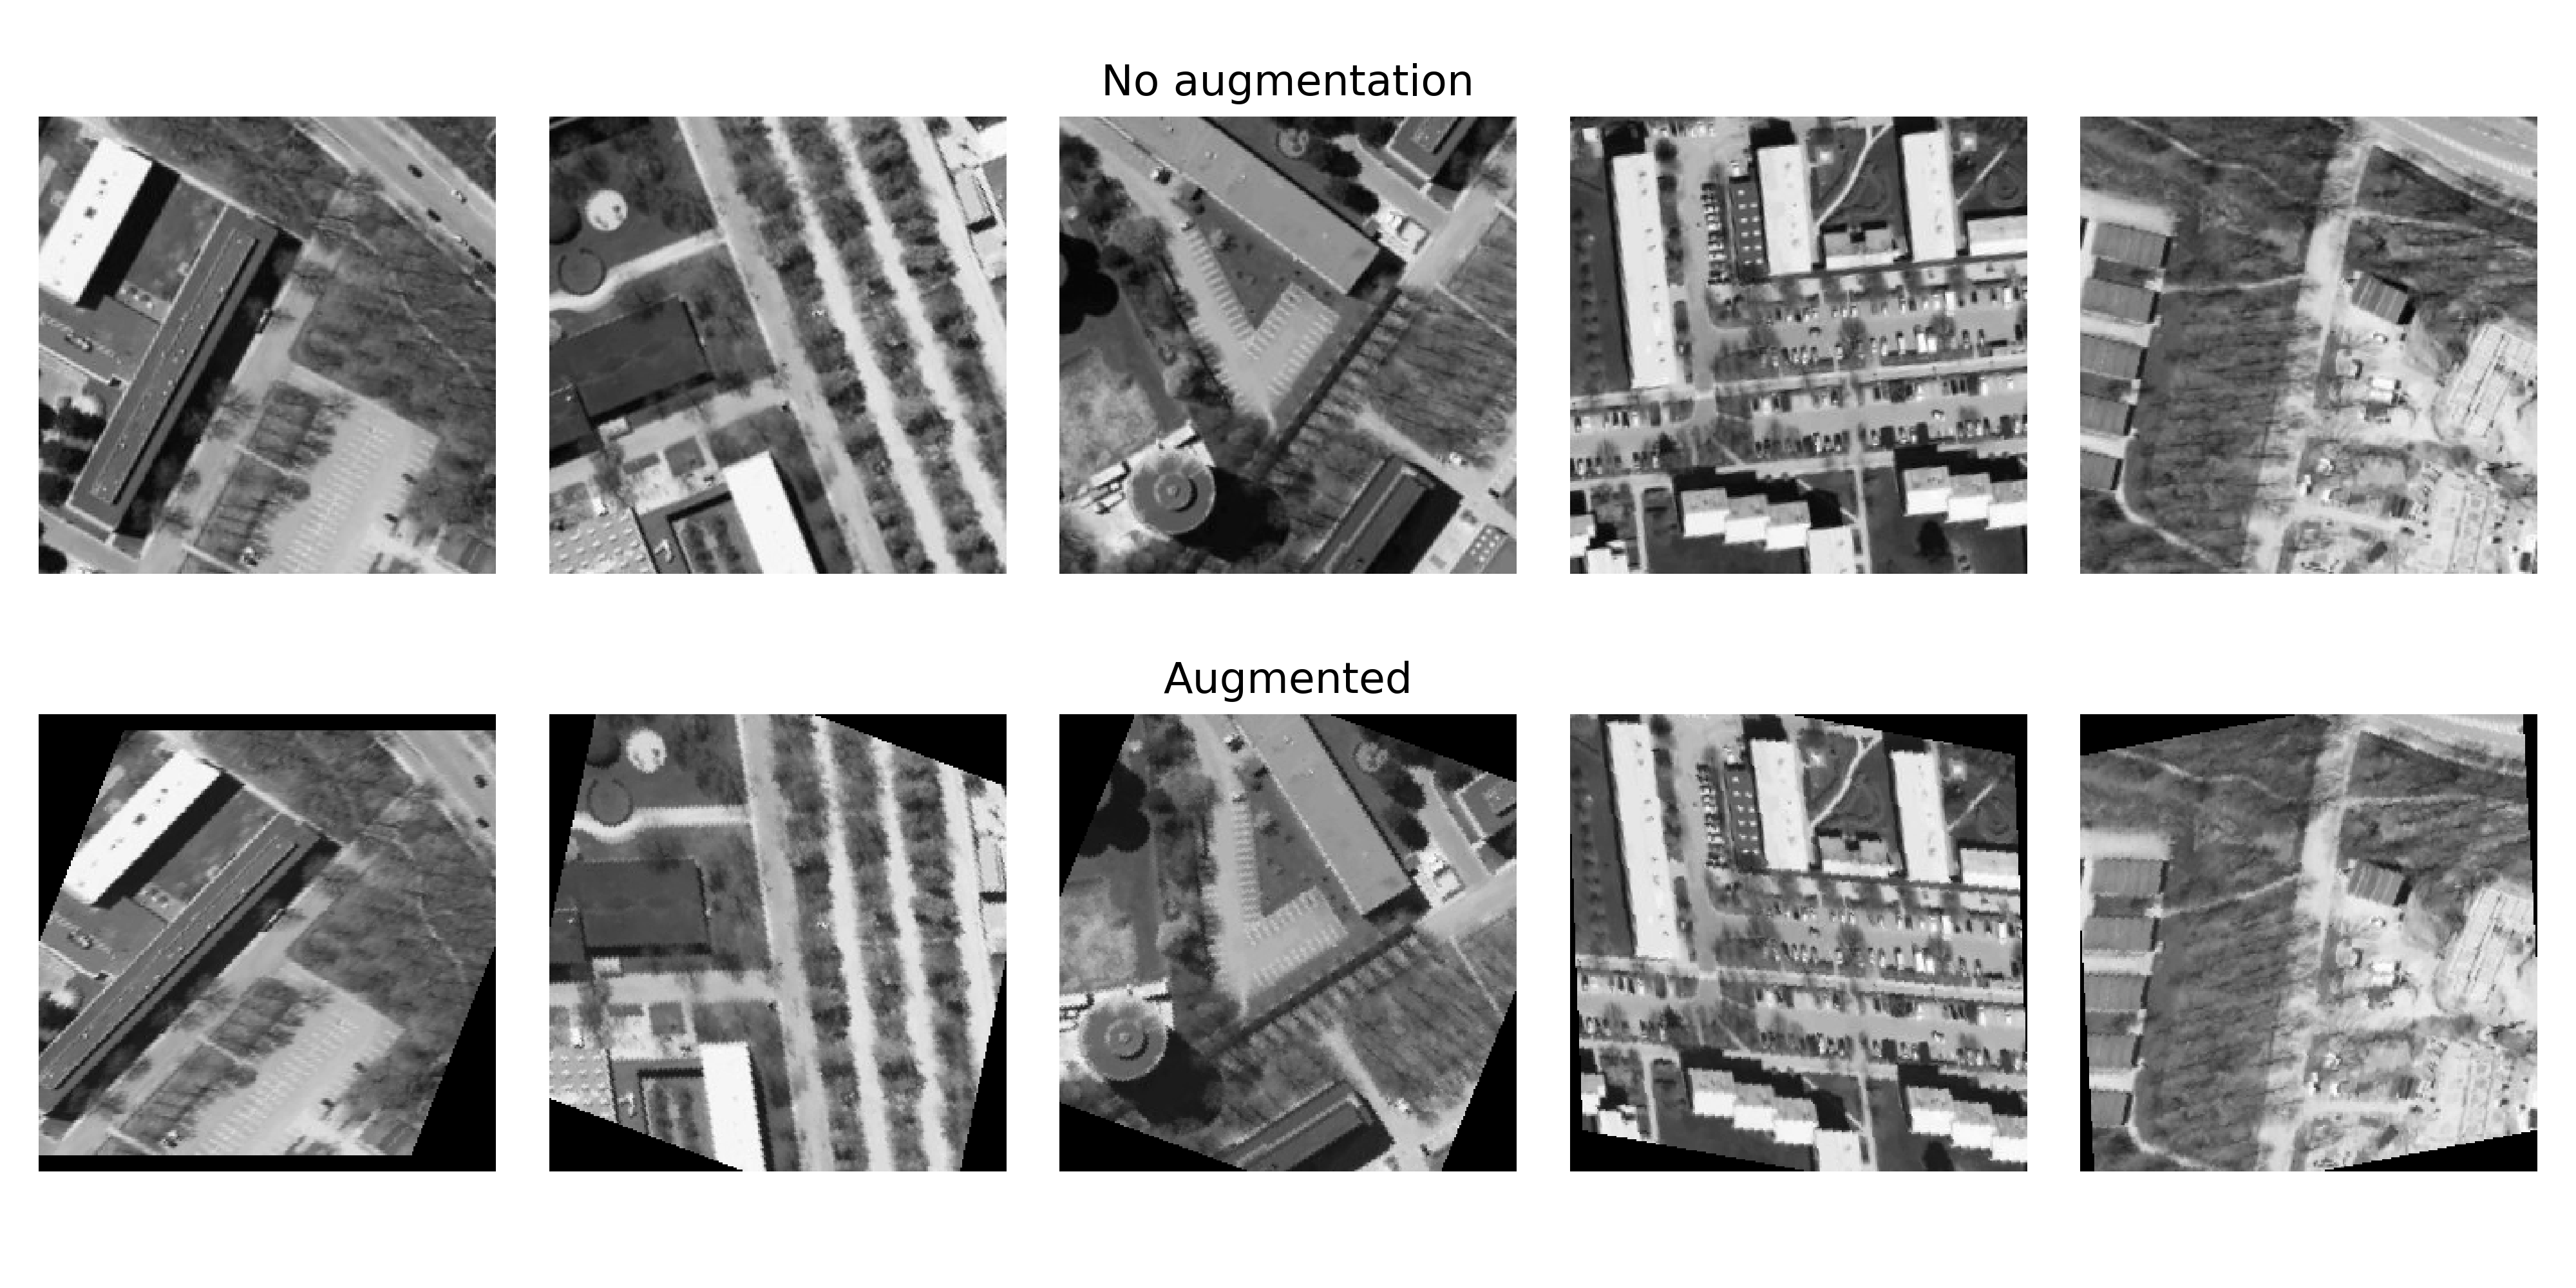
\includegraphics{chapters/part_pathloss/model_aided_paper/data_augmentation.png}
    \caption{A random affine transformation of satellite images used for data augmentation.}
    \label{fig:data_augmentation}
\end{figure}

A significant number of experiments were completed for scanning hyper-parameters. A complete list of hyper-parameters can be found in Table \ref{tab:cnn_structure}, \ref{tab:nn_structure} and \ref{tab:hyperparam_rest}. A total of $177$ experiments were conducted using different image strategies; the specific number of experiments can be observed in Table \ref{tab:experiments}. The scanning was done with a random search technique, meaning the hyper-parameters were sampled using a uniform distribution between ranges of interest \cite{Bergstra2012RandomOptimization}. A learning rate scheduler was applied with a patience parameter of $5$ epochs. Meaning, if no improvement in test error has been observed for at least five epochs, the learning rate is reduced with a factor of 10. This is also termed, \emph{reducing learning rate on plateu} and has been shown to improve the convergence of \glspl{nn} \cite{SmithSuper-Convergence:Rates}. The training is terminated when the learning rate reaches a value of $< 10^{-8}$.

\def\arraystretch{1.5}
\begin{table}[]
\begin{center}
\begin{tabular}{ll}
\multicolumn{2}{c}{\textbf{CNN}}                                                       \\
\multicolumn{1}{l|}{Input ch.}           & 1                                          \\ \hline
\multicolumn{1}{l|}{No. of convolutions} & [200, 100, 50, 25, 12, 1]                  \\ \hline
\multicolumn{1}{l|}{Activation}          & \emph{ReLU}                                       \\ \hline
\multicolumn{1}{l|}{Kernel size}         & [(5,5), (3,3), (3,3), (3,3), (2,2), (2,2)] \\ \hline
\multicolumn{1}{l|}{Max pooling}         & 2                                          \\ \hline
\multicolumn{1}{l|}{Padding}             & 2                                          \\ \hline
\multicolumn{1}{l|}{Stride}              & 1                                         
\end{tabular}
\end{center}
\caption{Architecture of the \gls{cnn} used for processing satellite images as detailed in Fig. \ref{fig:satellite_model_setup_v2}}\label{tab:cnn_structure}
\end{table}



\begin{table}
\subfloat[][]{
\begin{tabular}{ll}
\multicolumn{2}{c}{\textbf{NN}}                                                       \\
\multicolumn{1}{l|}{Layer size} & [200, 200]                  \\ \hline
\multicolumn{1}{l|}{Activation}          & \emph{ReLU}                                     
\end{tabular}
}
\subfloat[][]{
\begin{tabular}{ll}
\multicolumn{2}{c}{\textbf{NN2}}                                                       \\
\multicolumn{1}{l|}{Layer size} & [200, 16, 1]                  \\ \hline
\multicolumn{1}{l|}{Activation}          & \emph{ReLU}                                     
\end{tabular}
}
\vspace{1em}
\caption{Architecture of the sub-models considered in the final model architecture. }\label{tab:nn_structure}
\end{table}

\begin{margintable}
\begin{tabular}{@{}ll@{}}
\toprule
\textbf{Parameter} & \textbf{Value}   \\ \midrule
Batch size         & $30$             \\
Epochs             & $100$            \\
Image Size         & $256 \times 256$ \\
Learning Rate      & $0.001$            \\
Augmentation Angle & $\pm 20^{\circ}$ \\
Weight Decay       & $0.0029$         \\ \bottomrule
\end{tabular}
\caption{Best performing hyper-parameters for model \emph{v2}}\label{tab:hyperparam_rest}
\end{margintable}


\begin{table}[]
\centering
\begin{tabular}{@{}ll@{}}
\toprule
\textbf{Images} & \textbf{Experiments} \\ \midrule
Gray-scale images            & 114                  \\
Color images                 & 48                   \\
No data augmentation         & 15                   \\ \midrule
\textbf{Total}               & \textbf{177}         \\ \bottomrule
\end{tabular}
\caption{Number of experiments conducted for different image strategies.}\label{tab:experiments}
\end{table}


\subsection{Results}

The performance of the hyper-parameters weight decay and the augmentation angle is observed in Fig. \ref{fig:hyperparameters_weight_decay} (lower is better). A trend in an increase in performance is observed for both test and training, for decreasing values of weight decay. The trend for the augmentation angle is not as clear, as shown by the standard deviation and the mean of the experiments. Even though the mean observed performance of $10^{\circ}$ is better than the mean performance of $20^{\circ}$, the $\sigma$ at $20^{\circ}$ brings the overall test error closer to the training error. Thus the best performing model was found among the models trained at $20^{\circ}$ of data augmentation angle. The best performing found hyper-parameters can be seen in Table \ref{tab:hyperparam_rest}.

\begin{figure}
    \centering
    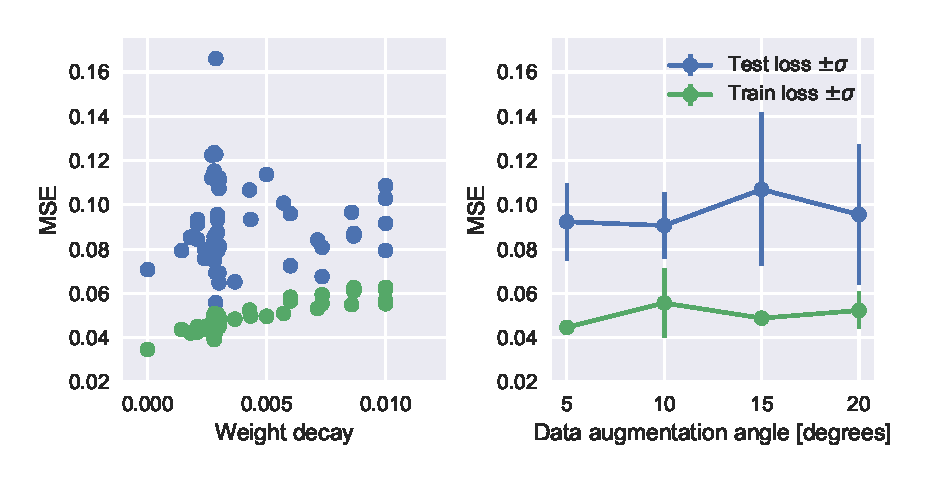
\includegraphics{chapters/part_pathloss/model_aided_paper/hyperparameters_grayscale.eps}
    \caption{Training and test error in MSE for weight decay and the augmentation angle.}
    \label{fig:hyperparameters_weight_decay}
\end{figure}


Using the traditional approaches of channel modelling, we can compare the performance. The comparison can be seen in terms of \gls{rmse} (lower is better) in Fig. \ref{fig:model_comparison_bar_group} for 811 and 2630 MHz respectively for the \uma{B} model and the ray-tracing model. The proposed approach is observed to outperform traditional modelling techniques for both 811 MHz and 2630 MHz, respectively. A gain of $\approx 1$ dB for 811 MHz, and $\approx 4.7$ dB for 2630 MHz is achieved compared to the traditional option, \uma{B}. 


\begin{figure}
    \centering
    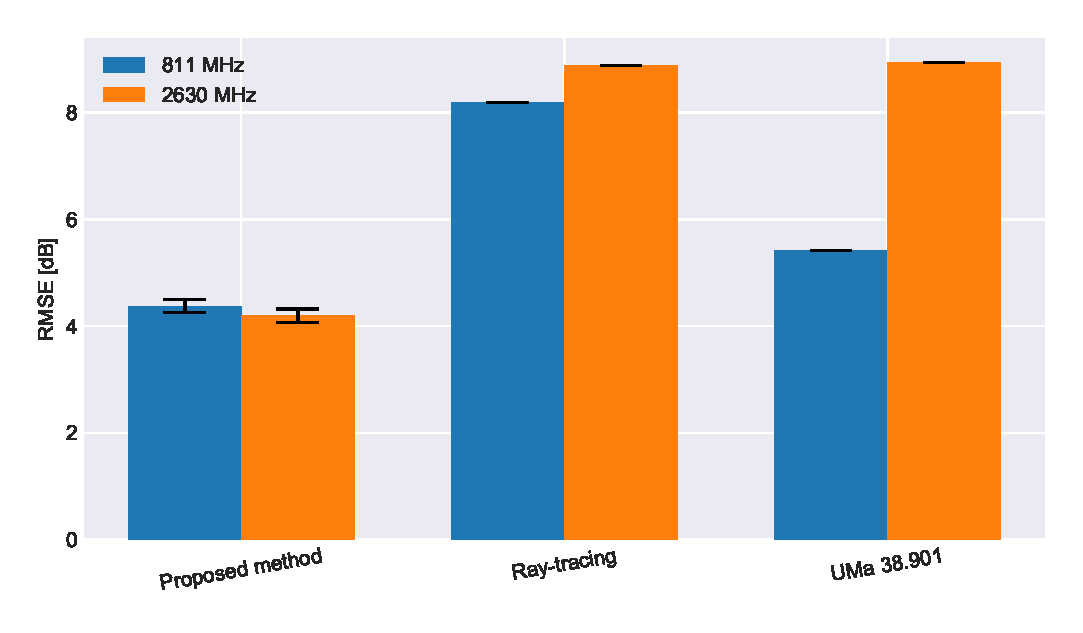
\includegraphics{chapters/part_pathloss/model_aided_paper/model_comparison_bar_group_std_split.eps}
    \caption{RMSE performance at 811 MHz and 2630 MHz for the proposed model \emph{v2} compared to traditional modelling techniques.}
    \label{fig:model_comparison_bar_group}
\end{figure}

The performance of the model is investigated in Fig. \ref{fig:train_models_barplot} where different versions of the proposed model are compared. More specifically, 1) no inclusion of a simple path loss (e.g. only data-driven), 2) no use of images (e.g. only features) and 3) with the aid from a simple path loss model and images (e.g. the complete proposed model). The \gls{rmse} in predictive performance, by including and processing satellite images, is  $\approx 4.37$ dB and $\approx 4.19 $ dB for $811$ and $2630$ MHz respectively. Meanwhile only using the features and being completely data-driven (e.g. no images or convolutional neural network and not aided by the path loss model) offer a performance of $\approx 5.12$ and $\approx 4.9$ dB for $811$ MHz and $2630$ MHz respectively. 

The introduction of the simple path loss model improves 1) the standard deviation of the predictive error and 2) the predictive performance. The standard deviation of the predictive error is the result of training multiple models with the same hyper-parameters, although instantiated with random weights. It can be seen as the error bars in Fig. \ref{fig:train_models_barplot}. By aiding the training process with a simple path loss model, the standard deviation of predictive performance was reduced from $\approx 0.57$ to $\approx 0.05$ dB. The performance increase can be observed to be $\approx 0.19$ and $\approx 0.54$ dB for 811 and 2630 MHz respectively comparing the fully data-driven approach and the introduction of a simple path loss model. 

The observed performance of the complete model (thus the use of satellite images and aided by a path loss model) increases the predictive performance, however with a slight increase in the standard deviation of prediction. More specifically, the gain provided by including images (compared to only using features) can be observed to be $\approx 0.55$ and $\approx 0.15$ for $811$ and $2630$ MHz respectively. The standard deviation increased to $\approx 0.05$ to $\approx 0.12$ dB. 

In summary, aiding the model with a path loss model improved the predictive capability by $\approx 0.54$ dB at $2630$ MHz while a reduced improvement was seen at $811$ MHz of $\approx 0.19$ dB. Including the images improved performance additionally by $\approx 0.55$ dB at $811$ MHz and $\approx 0.15$ dB at $2630$ MHz.

\begin{figure}
    \centering
    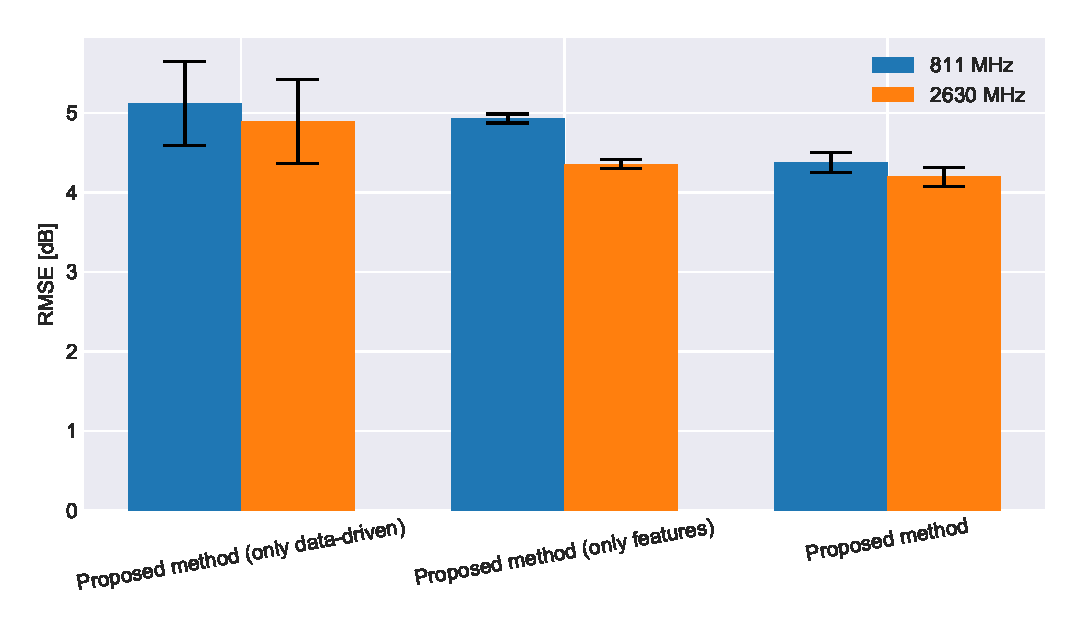
\includegraphics{chapters/part_pathloss/model_aided_paper/trainedmodels_barplot.eps}
    \caption{Comparison of different model techniques and structures.}
    \label{fig:train_models_barplot}
\end{figure}

The result of applying data augmentation can be observed in Fig. \ref{fig:dataaugmentation_training_test_error}. The test set is evaluated for each training epoch, thus providing the test and training error with and without data augmentation. A significant reducing in the generalization gap is observed and reduced from $\sim 0.13$ to $< 0.09$. 

\begin{figure}
    \centering
    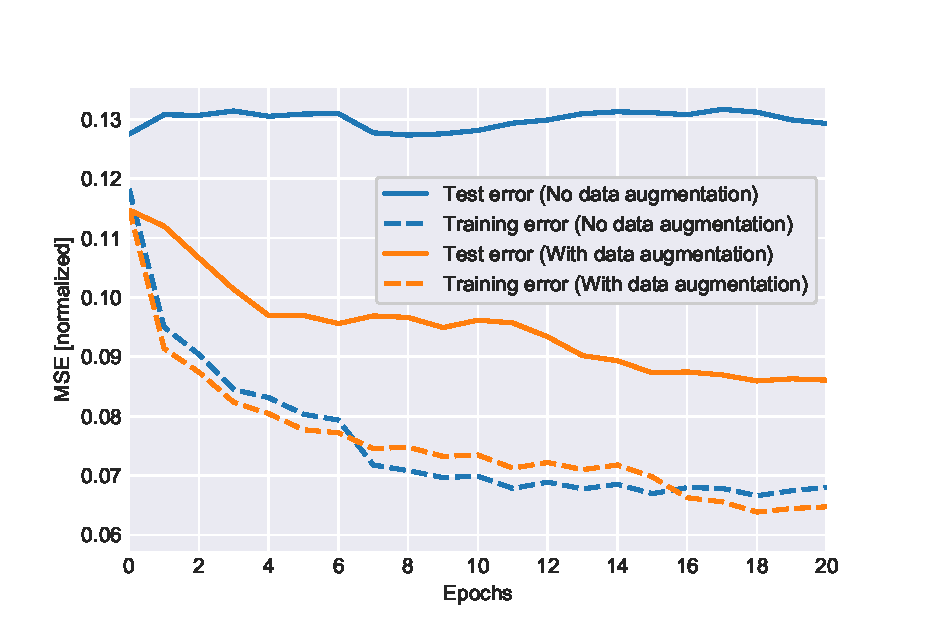
\includegraphics{chapters/part_pathloss/model_aided_paper/dataaugmentation_training_test_error.eps}
    \caption{The test and training error evaluated with and without the use of data augmentation techniques.}
    \label{fig:dataaugmentation_training_test_error}
\end{figure}

The output of $z(\cdot)$ as noted by Eq. (\ref{eq:model}) can be observed in Fig. \ref{fig:rsrp_correction_hist} for both 811 and 2630 MHz. The Deep Learning model produces thus a correction-element to the simple link budget estimation. The correction is similar to a Gaussian distribution, which is the model prerequisite and also how large-scale fading can be modelled. It should be noted that the distributions are not entirely centred, which illustrates a calibration offset. No gain was observed in re-calibrating the model such the mean was centred around $0$, e.g. $\mathcal{N}(0, \sigma)$.

\begin{figure}
    \centering
    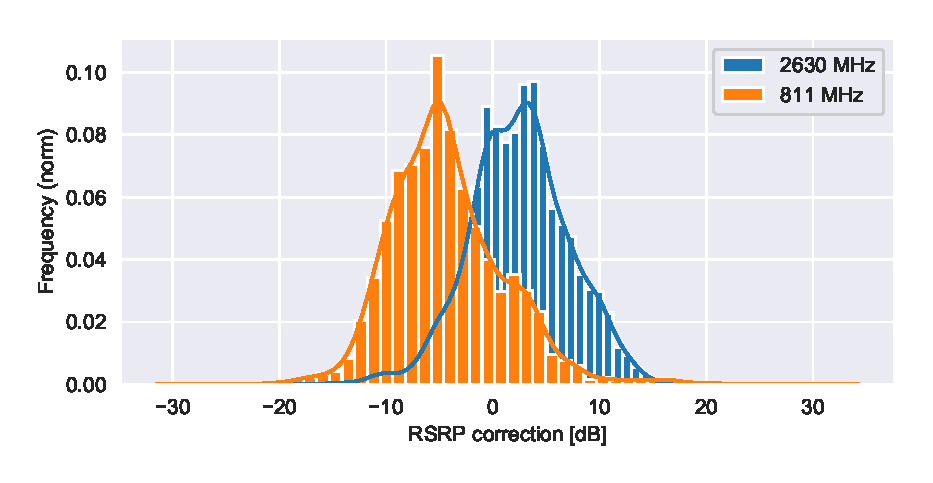
\includegraphics{chapters/part_pathloss/model_aided_paper/rsrp_correction_hist.eps}
    \caption{RSRP correction as noted by the output of $z(\cdot)$ in Eq. (\ref{eq:model}).}
    \label{fig:rsrp_correction_hist}
\end{figure}

The distributions of the \gls{rsrp} measurements and the prediction can be seen in Fig. \ref{fig:dist_pred_target} for both 811 and 2630 MHz. The performance difference between 811 and 2630 MHz, (as visualized by Fig. \ref{fig:model_comparison_bar_group}) comes to show here. A visually pleasing fit between predicted and measured is observed for 2630 MHz, while at 811 MHz, the model have issues with values of \gls{rsrp} around $-100$ to $-90$ dBm.

\begin{figure}
    \centering
    \subfloat[811 MHz]{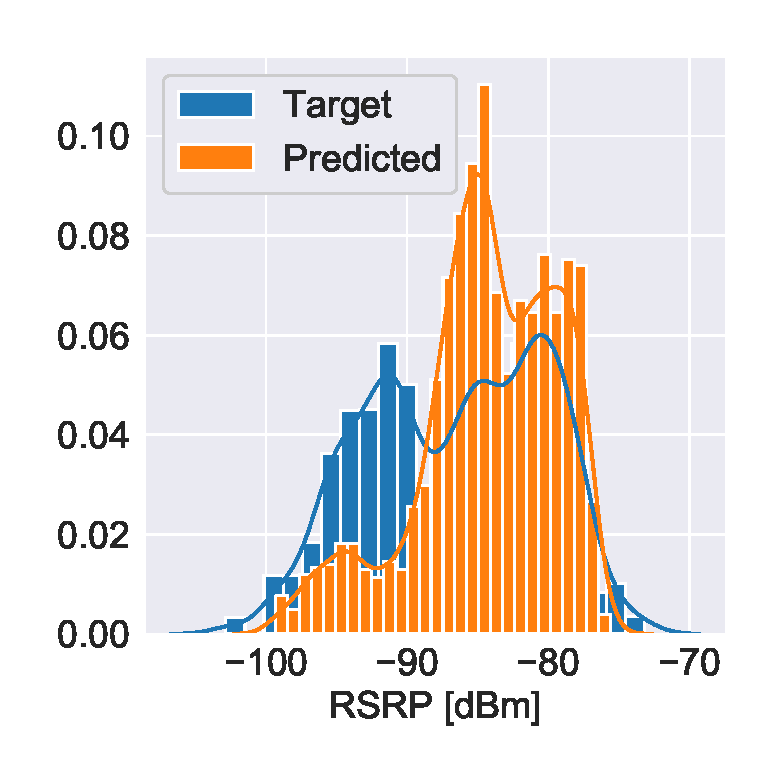
\includegraphics[width=0.4\textwidth]{chapters/part_pathloss/model_aided_paper/hist_63b17fa0-89e0-440b-952c-aa7f2e63e49c_811mhz.eps}\label{fig:dist_811}}  
    \subfloat[2630 MHz]{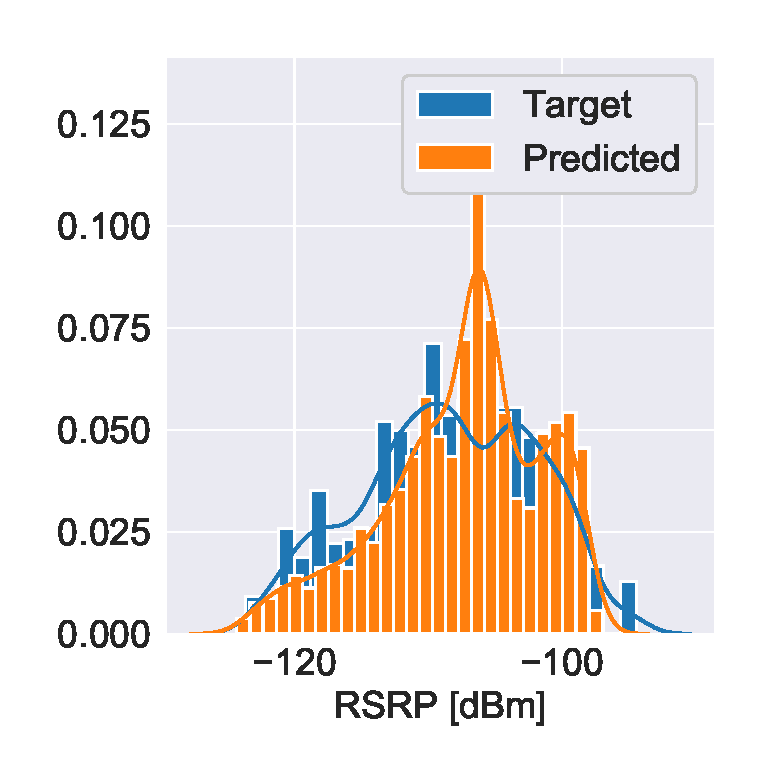
\includegraphics[width=0.4\textwidth]{chapters/part_pathloss/model_aided_paper/hist_63b17fa0-89e0-440b-952c-aa7f2e63e49c_2630mhz.eps}\label{fig:dist_2630}}
    \caption{Distribution of RSRP for 811 (a) and 2630 (b) MHz on the test set and the model output.}
    \label{fig:dist_pred_target}
\end{figure}

\subsection{Discussion}
The proposed approach is capable of outperforming traditional methods such as ray-tracing and empirical models. The predictive performance improvement at $2630$ MHz is $\approx 4.7$ dB while $\approx 1$ dB of gain is achieved at 811 MHz. The performance at 2630 MHz indicates the necessity of data describing local variability, which is not present in either the implemented ray-tracing model (limited clutter detail) or the empirical model. Clutter data is, however, observable in the proposed satellite images. The result indicates that this is not solely caused by including satellite images. The specific performance gain offered by the inclusion of the images is documented to be, on average, $\approx 0.8$ dB. Thus, the performance increase (compared to the traditional methodologies) seem to overall indicate the usefulness of \gls{nn} in path loss predictions. The majority of the performance increase is not caused by the inclusion of satellite images but rather the adaptive nature of \gls{nn}. However, by including the images and aiding the model with a simple path loss model, additional improvements to performance are achieved. 

The area spanned by the image offer details of clutter, nearby buildings and even parked cars. However, the area spanned by the images might contain details not relevant to differences in frequency. For instance, higher attenuation is associated with higher frequencies when it comes to clutter data due to the lower wavelength. In this case, it might be more relevant to include a more detailed version of the image spanning a reduced area. Moreover, it might be that the images simply contain too much information necessary for relevant propagation statistics. Such insight was gained during the hyper-parameter scanning, of which many experiments were conducted. Likely, simplistic images or the vectorization of such images (e.g. footprints/outlines of buildings) may improve the predictive performance, or in any case, enhance the task of finding the best-performing hyper-parameters.

The task of hyper-parameter scanning is complex and time-consuming. From the results, it is clear that performance improvements have been achieved in both utilizing features, a simple path loss model and satellite images. However, it should be noted that the documented hyper-parameters is an attempt at an optimum solution. It is likely that better hyper-parameters can be found using extensive scanning and possibly even Machine Learning-based sampling methodologies as documented in Chapter \ref{ch:mlbasics}. The model achieved requires approximately 300 experiments, each with 240 minutes of training time. The amount of experiments completed leads to the discussion of complexity. It is argued that the proposed method requires reduced complexity as compared to a traditional ray-tracing approach. The geostatistics and data necessary for local variability approximations are embedded into the supplied images and requires only the convolution and multiplication operations for extracting the \emph{correction} to a predicted path loss. It can be argued that the model only needs to be trained once, upon discovery of the best hyper-parameters. So in short, the complexity of the trained method solely lies in the prediction time and the memory necessary hereof. 

\subsection{Conclusion}\label{subsec:conclusion_v2}
The introduction of a simple path loss model (expert knowledge) for aiding the training process, in combination with satellite images, have improved the overall generalization properties of the Deep Learning model. The study items identified in \emph{version 1} have successfully been explored in an attempt to quantify the properties of the proposed approach and achieve insight into the specific prediction improvements by including satellite images. Furthermore, compare how the method performs to traditional approaches. The technique is capable of improving prediction accuracy by $\approx 1$ dB at $811$ MHz and $4.7$ dB at $2630$ MHz. The model provides an average prediction error of $\approx 4.1$ dB when predicting \gls{rsrp} in an unseen area for both $811$ and $2630$ MHz, which is a significant improvement to traditional methodologies. It is furthermore concluded that the complexity of the model is primarily associated with the untrained model, e.g. hyper-parameters and the selection hereof. The trained model is capable, with only position and available satellite images to produce an accurate prediction of receiver power in unseen areas.


\section{Reduced image complexity (v3)}\label{sec:osm_v3}
The implication of utilizing both satellite images and expert knowledge (in terms of a path loss model) requires further investigation and explorations. In particular, it is of interest to effectively reduce the model complexity to enable a more transparent inference of the prediction capability. Additionally, and possibly, more importantly, it is of great interest to validate the approach by using inherently different data sources. 

In the work \cite{Thrane2020DeepKnowledge}, the proposed approach is validated using simplified geographical images and additional drive test data. More specifically, this includes the use of so-called \emph{OpenStreetMap} data to supply the needed information for the used images. Furthermore, to enable generalization and interpolation between inherently different data sources, some changes were conducted to the features. The approach of this is visualized in Fig. \ref{fig:version3_architecture_figure}.

\begin{figure*}
    \centering
    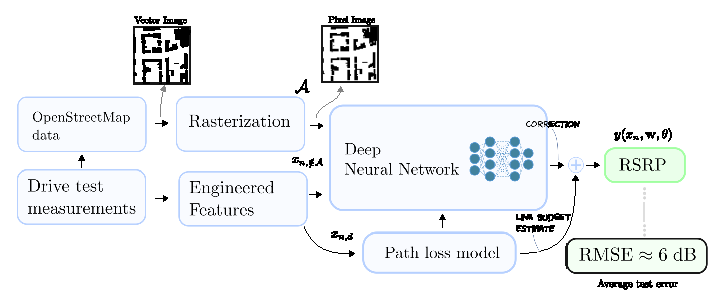
\includegraphics{chapters/part_pathloss/osm_images_paper/figures/version3_architecture_figure.eps}
    \caption{Architecture is set to utilize images provided by \gls{osm} instead of satellite images.}
    \label{fig:version3_architecture_figure}
\end{figure*}




\subsection{German measurements}

The experimental measurements of the previously used drive test data (See appendix \ref{app:drive_test_study_2017}, \cite{1xf4-eg98-19}) is appended with data from Dortmund, Germany \cite{SliwaEmpiricalNetworks}. The dataset contains measurements from multiple \glspl{mno} in different propagation scenarios at different operating frequencies. The essential characteristics can be seen in Table \ref{tab:drive_test_data_total}. The fundamental characteristics of the data allow for engineering the relevant features required for applying the proposed \gls{dl} model.

\begin{table*}[h]
\footnotesize
\begin{tabular}{@{}llll@{}}
\toprule
Dataset      & Samples & MNOs & Frequencies  [MHz]       \\ \midrule
DK Campus    & $57586$   & $1$    & $[811, 2630]$ \\
GER Campus   & $8579$    & $3$    & $[850, 860, 1815, 1845, 1865, 2630]$                   \\
GER Urban    & $11921$   & $3$    &  $[850, 860, 1845, 1865, 2630, 2650, 2680]$ \\
GER Suburban & $27152$   & $3$    &  $[850, 860, 1815, 1845, 1865,2630]$                   \\
GER Highway  & $20662$   & $3$    & $[850, 860, 870, 950, 1815, 1845, 1865,2630]$                    \\ \midrule
Total        & $125900$  &      &                     \\ \bottomrule
\end{tabular}
\vspace{1em}
\caption{Additional drive test data is available for training and testing consisting of various transmission frequencies.}\label{tab:drive_test_data_total}
\end{table*}

\subsection{Methodology}\label{subsec:osm_methodology}

Upon initial prototyping of the proposed method, it was found that the general features of \gls{gnss} positions, e.g. latitude and longitude coordinates caused severe extrapolation issues. More specifically, the model attempted to interpolate between the coordinates. The importance of the coordinates to the prediction of \gls{rsrp} caused the model to learn latent features of spatial importance. When evaluating the methodology in a different region (significant difference in latitude and longitude coordinates), the trained model would then provide a wrong interpretation of the spatial features by interpolating between coordinates. For this reason, a few changes to the formalized of the required engineered features were made. More specifically this resulted in

\begin{equation}
    x_n = [v, d, \Delta_\text{lat}, \Delta_\text{lon},  f_c, \mathcal{A}]
\end{equation}

Where $v$ is the velocity of the vehicle, $d$ is the distance in $3$D, $\Delta_\text{lat}$, $\Delta_\text{lon}$ are the difference in latitude and longitude between the receiver and the \gls{enb} respectively. $f_c$ is the carrier frequency in MHz, and $\mathcal{A}$ is the new simplified image.

The image was constructed similarly as \emph{v1} and \emph{v2}, using a \gls{roi} and a rotation towards the transmitter. Instead of the rotation causing the transmitter to be direction south (down) in the image, the image was rotated such that a direct path is to the east (right) in the image. Any performance gains did not cause this change, but rather ease of implementation. An example of such an image can be seen in Fig. \ref{fig:roi_image_preperation}. The area spanned by the image was adjusted to find the optimum use of the images. The rasterized image was kept constant at a size of $64 \times 64$ pixels. The images were extracted with the tool as documented in \cite{SliwaLightweightNetworks}. Data augmentation, as discussed in Section \ref{sec:training_v2}, was applied similarly.


\begin{figure}
    \centering
    
\includegraphics{chapters/part_pathloss/osm_images_paper/figures/map_to_image.eps}
    \caption{The \gls{roi} was determined around the measurement position spanning a variable size of area covered.}
    \label{fig:roi_image_preperation}
\end{figure}

\subsection{Model architecture}

The model architecture was kept similar to the one used in \emph{v2} embedding expert knowledge of path loss. A change to model complexity was necessary due to the simplification of 1) the engineered features and 2) the geographical images. The general idea of the model architecture is identical to that of Fig. \ref{fig:combined_model_approach} and Fig. \ref{fig:satellite_model_setup_v2}. The reduction in model complexity resulted in a significant increase in the number of hyper-parameters scanned and the automatization hereof. A Bayesian optimization scheme was applied to find the most probable hyper-parameters given the weight space provided by the final test error \cite{YuHyper-ParameterApplications, wandb}. Over $500$ experiments of different hyper-parameters and combinations hereof was conducted, resulting in a large model complexity reduction. An example of the hyper-parameter experiments can be found in Fig. \ref{fig:hyper-paramters_scan}. The final achieved hyper-parameters can be found in Table \ref{tab:hyper-parameters}.

Specifically, a reduction of convolutional filters can be observed. For instance, the first layer of the \gls{cnn} is reduced with $\approx 170$ filters compared to \emph{v2}. Furthermore, the size of the fully-connected layers processing the engineered features has also seen a reduction from $200$ to $32$. Additionally, the last \gls{nn} sub-module has been reduced from $200$ to $16$. This reduction has reduced not only the memory footprint of the proposed model but also the training performance and thus the resulting inference performance. Specifically, the model complexity reduction has resulted in sub-millisecond prediction times (accelerated with a GPU). 

\begin{figure*}
    \centering
    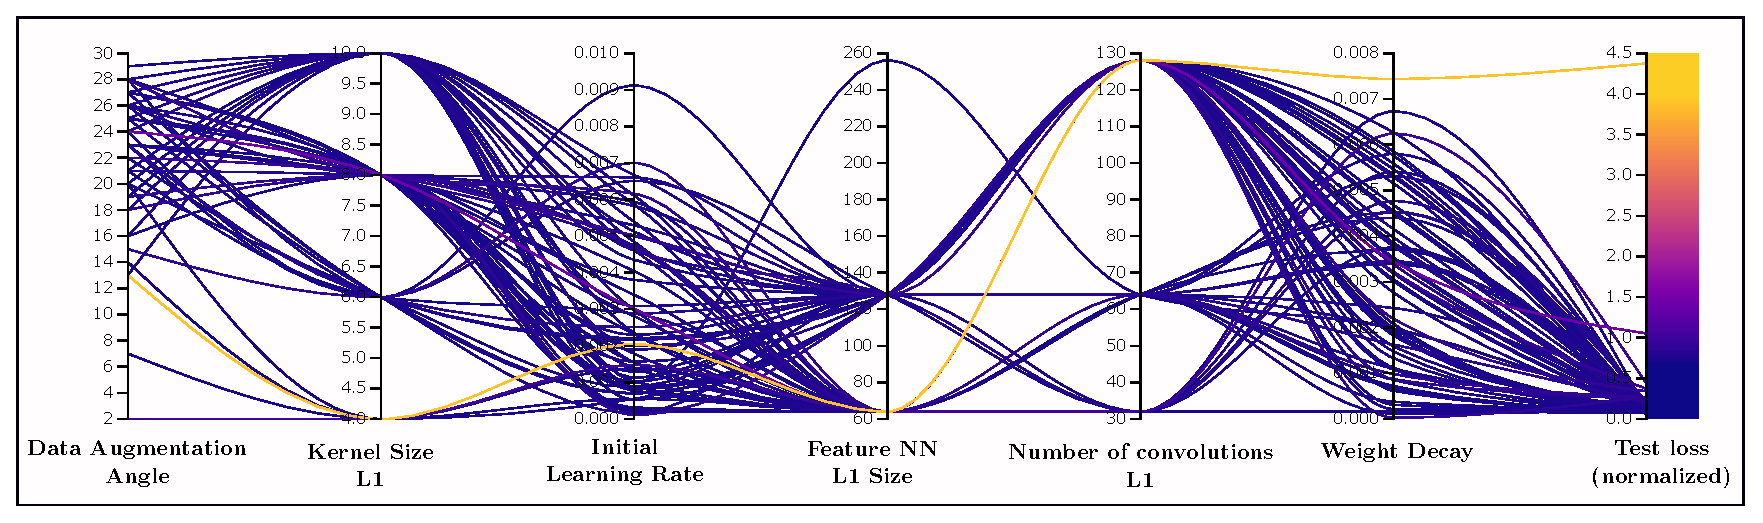
\includegraphics{chapters/part_pathloss/osm_images_paper/figures/hyperparameter_scan.eps}
    \caption{Bayesian optimization applied during hyper-parameter scan \cite{wandb}.}
    \label{fig:hyper-paramters_scan}
\end{figure*}


\begin{table}[]
    \centering
    \footnotesize
    \caption{Hyper-parameters for the deep neural network model.}\label{tab:hyper-parameters}
    \begin{tabular}{@{}lll@{}}
    \toprule
    \textbf{Parameter}          & \textbf{Value}                &  \\ \midrule
    Weight decay                & 8e-4                          &  \\
    Learning rate               & 1e-3                          &  \\
    Filters                     & [32, 32, 10, 1]               &  \\
    Kernel size                 & [(5,5), (3,3), (3,3), (2,2)]  &  \\
    Max pooling                 & [2, 2, 2, 2]                  &  \\
    Feature NN layer size       & [32, 32]                      &  \\
    Output NN layer size        & [16, 16]                      & \\
    Image augmentation angle    & 20                            & \\
    Image size                  & $64~\text{px} \times 64~\text{px}$                & \\
    Batch size                  & 12                            &  \\ \bottomrule
\end{tabular}
\end{table}

\newpage
\newpage


\subsection{Comparative results}
The results of utilizing simple geographical images instead of the satellite images can be seen in Fig. \ref{fig:model_comparison_access}. The overall performance can be seen to be identical to that of \emph{v2} on the same test set. A slight decrease at 811 MHz in performance is observed, however with a slight difference in the standard deviation across several version of the final trained models. Similar performance at $2630$ MHz was achieved.

\begin{figure}[h]
    \centering
    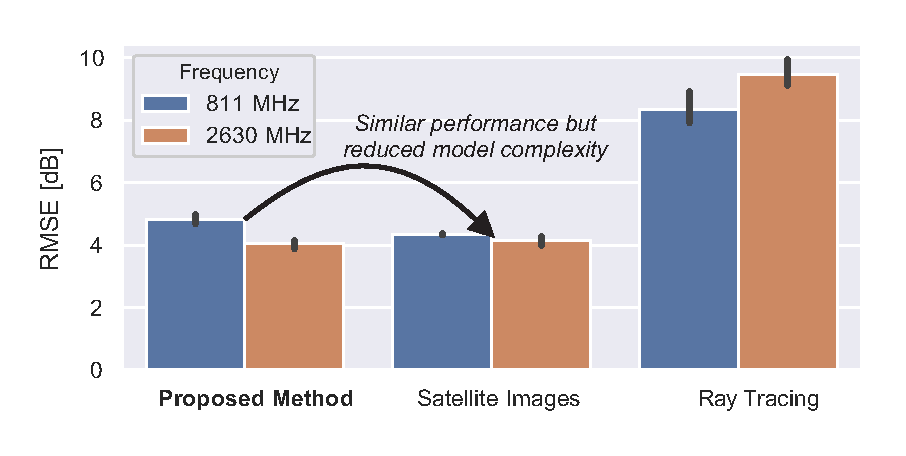
\includegraphics{chapters/part_pathloss/osm_images_paper/figures/model_comparison_access.eps}
    \caption{Comparison of simple \gls{osm} images with satellite images and ray-tracing.}
    \label{fig:model_comparison_access}
\end{figure}


To further explore the performance across all of the data subsets, a cross-validation approach was employed. Specifically, this entailed training on the majority of subsets while keeping one scenario for testing, repeated for all subsets. For instance, when refereed to the performance of \texttt{GER Campus} - it is trained on all other subsets of data excluding the \texttt{GER Campus} subset. The generalization gap for all subsets can be seen in Fig. \ref{fig:generalization_gap}. The figure shows the difference between the test and training error for each training epoch; in other words, how well the trained model performs on the remaining subset. If close to zero a generalization across the data subset is achieved. It can be seen that the \texttt{GER Campus} subset achieves by far the best generalization performance. The worst generalization is achieved for the \texttt{DK campus} subset. Both the \texttt{GER suburban} and \texttt{GER urban} subset achieved similar performance.

\begin{figure}[h]
    \centering
    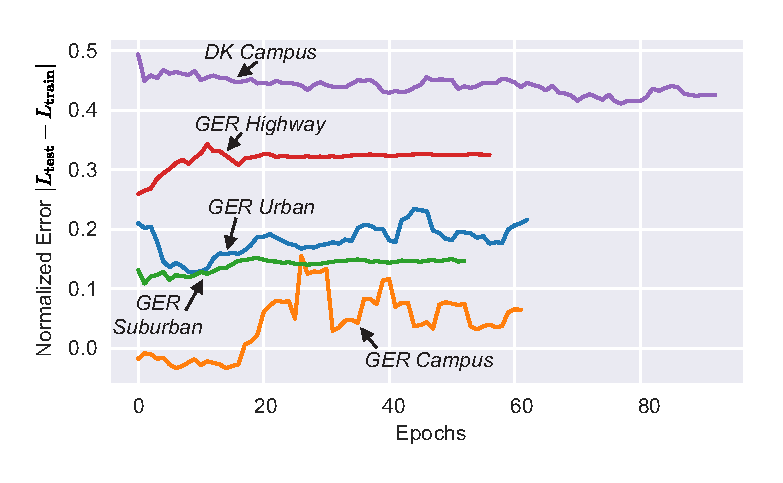
\includegraphics{chapters/part_pathloss/osm_images_paper/figures/training_test_error_crossvalidation_diff.eps}
    \caption{Generalization gap for all subsets.}
    \label{fig:generalization_gap}
\end{figure}

The performance is also evaluated in terms of \gls{rmse} (see \ref{eq:rmse}). This can be observed in Fig. \ref{fig:rmse_boxplot_osm} (lower is better). The cross-validated performance is shown for all subsets. The \gls{rmse} is computed for all mini-batches of samples, thus the figure shows the average \gls{rmse} across all mini-batches and the resulting standard deviation. Furthermore, outliers are also displayed. The best performance is achieved on the \texttt{GER campus} subset with a \gls{rmse} of $6.3$ dB and $\sigma = 3.6$ dB. The worst performance is seen on the \texttt{GER Highway} subset, with an \gls{rmse} of $9.7$ dB and $\sigma = 1.2$ dB.


\begin{figure}[h]
    \centering
    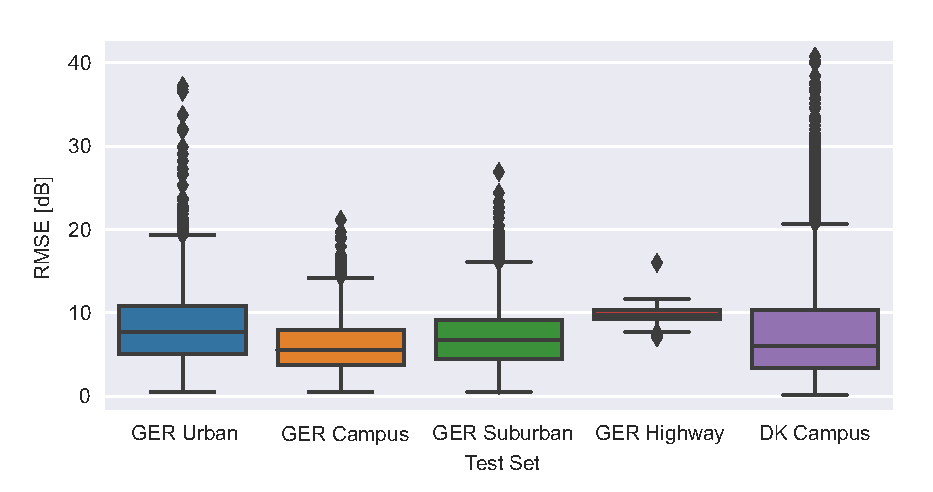
\includegraphics{chapters/part_pathloss/osm_images_paper/figures/RMSE_boxplot.eps}
    \caption{Cross-validation results of all data subsets. Each subset is evaluated using a model trained on the remainder of the subsets.}
    \label{fig:rmse_boxplot_osm}
\end{figure}

\subsection{Image distance results}
As a result of the reduced model complexity, additional exploration of the importance of spatial dependency has been completed. This has resulted in the comparison of so-called \emph{full-size} images instead of the \emph{regular} \gls{roi} images (centered around the measurement coordinate). The \emph{full-size} images consider not only the receiver location but also the transmitter location. In other words, both positions are within the spanned \emph{full-size} image. Thus, if the antenna separation distance increase, the area spanned by the image increase.  \emph{Regular} images have a constant area covered by the image regardless of antenna separation distance. A so-called \emph{violin} plot is found in Fig. \ref{fig:rmse_violin_image_comparison}. The figure shows the estimation of the kernel density provided by batch-wise \gls{rmse} computation. The distribution and range of using \emph{full-size} images are noticeably different than using the \emph{regular} images spanning 250 meters. More so, the number of outliers (and the range) increased. Using \emph{regular} images resulted in an \gls{rmse} of $6.3$ dB while an \gls{rmse} of $7.3$ dB was achieved using the \emph{full-size} images.



\begin{figure}[h]
    \centering
    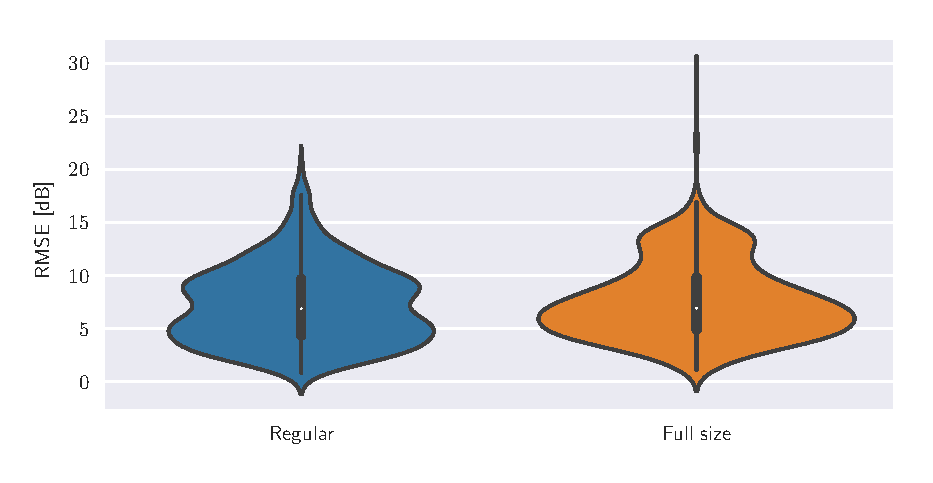
\includegraphics{chapters/part_pathloss/osm_images_paper/figures/RMSE_violin.eps}
    \caption{Performance comparison of varying the area spanned by the images. Evaluated on \texttt{GER Campus}, trained on the remainder.}
    \label{fig:rmse_violin_image_comparison}
\end{figure}


The impact of the area spanned by the \gls{roi} is evaluated in Fig. \ref{fig:boxplot_ci_image_distance}. The area spanned by the images are varied, while the pixel size of the image is kept constant. The performance is evaluated concerning the \texttt{GER Campus} subset, with a model trained on the remainder of the subsets. The best performing images were found spanning a distance of $250-300$ meters with similar predictive performance. Decreasing the distance spanned by the images offers a slight increase in \gls{rmse}. The same is observed for increasing the distance spanned by the images.

\begin{figure}
    \centering
    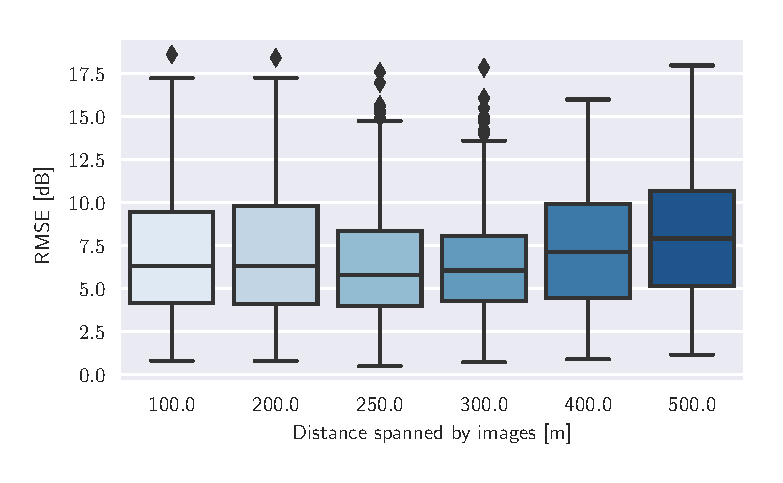
\includegraphics{chapters/part_pathloss/osm_images_paper/figures/boxplot_ci_image_distance.eps}
    \caption{Performance comparison of utilizing different distances for the images. The performance is with respect to the \texttt{GER Campus} subset, trained on the remainder.}
    \label{fig:boxplot_ci_image_distance}
\end{figure}

\subsection{Heatmap generation}

The trained models can effectively extrapolate and interpolate measurements in the area of the originated drive tests. An example of this for 2630 MHz can be seen in Fig. \ref{fig:osm_heatmap}. The model is trained on the entirety of the data points in the \texttt{DK Campus} subset. A grid of features is generated for all latitude and longitude coordinates in the area of interest. The model is then evaluated for the generated features. The results show a feasible range of predicted \gls{rsrp} values, in the range of $-80$ to $-140$ dBm. Furthermore, an increase in \gls{rsrp} is seen near the \gls{enb} location. 

\begin{figure}[!h]
    \centering
    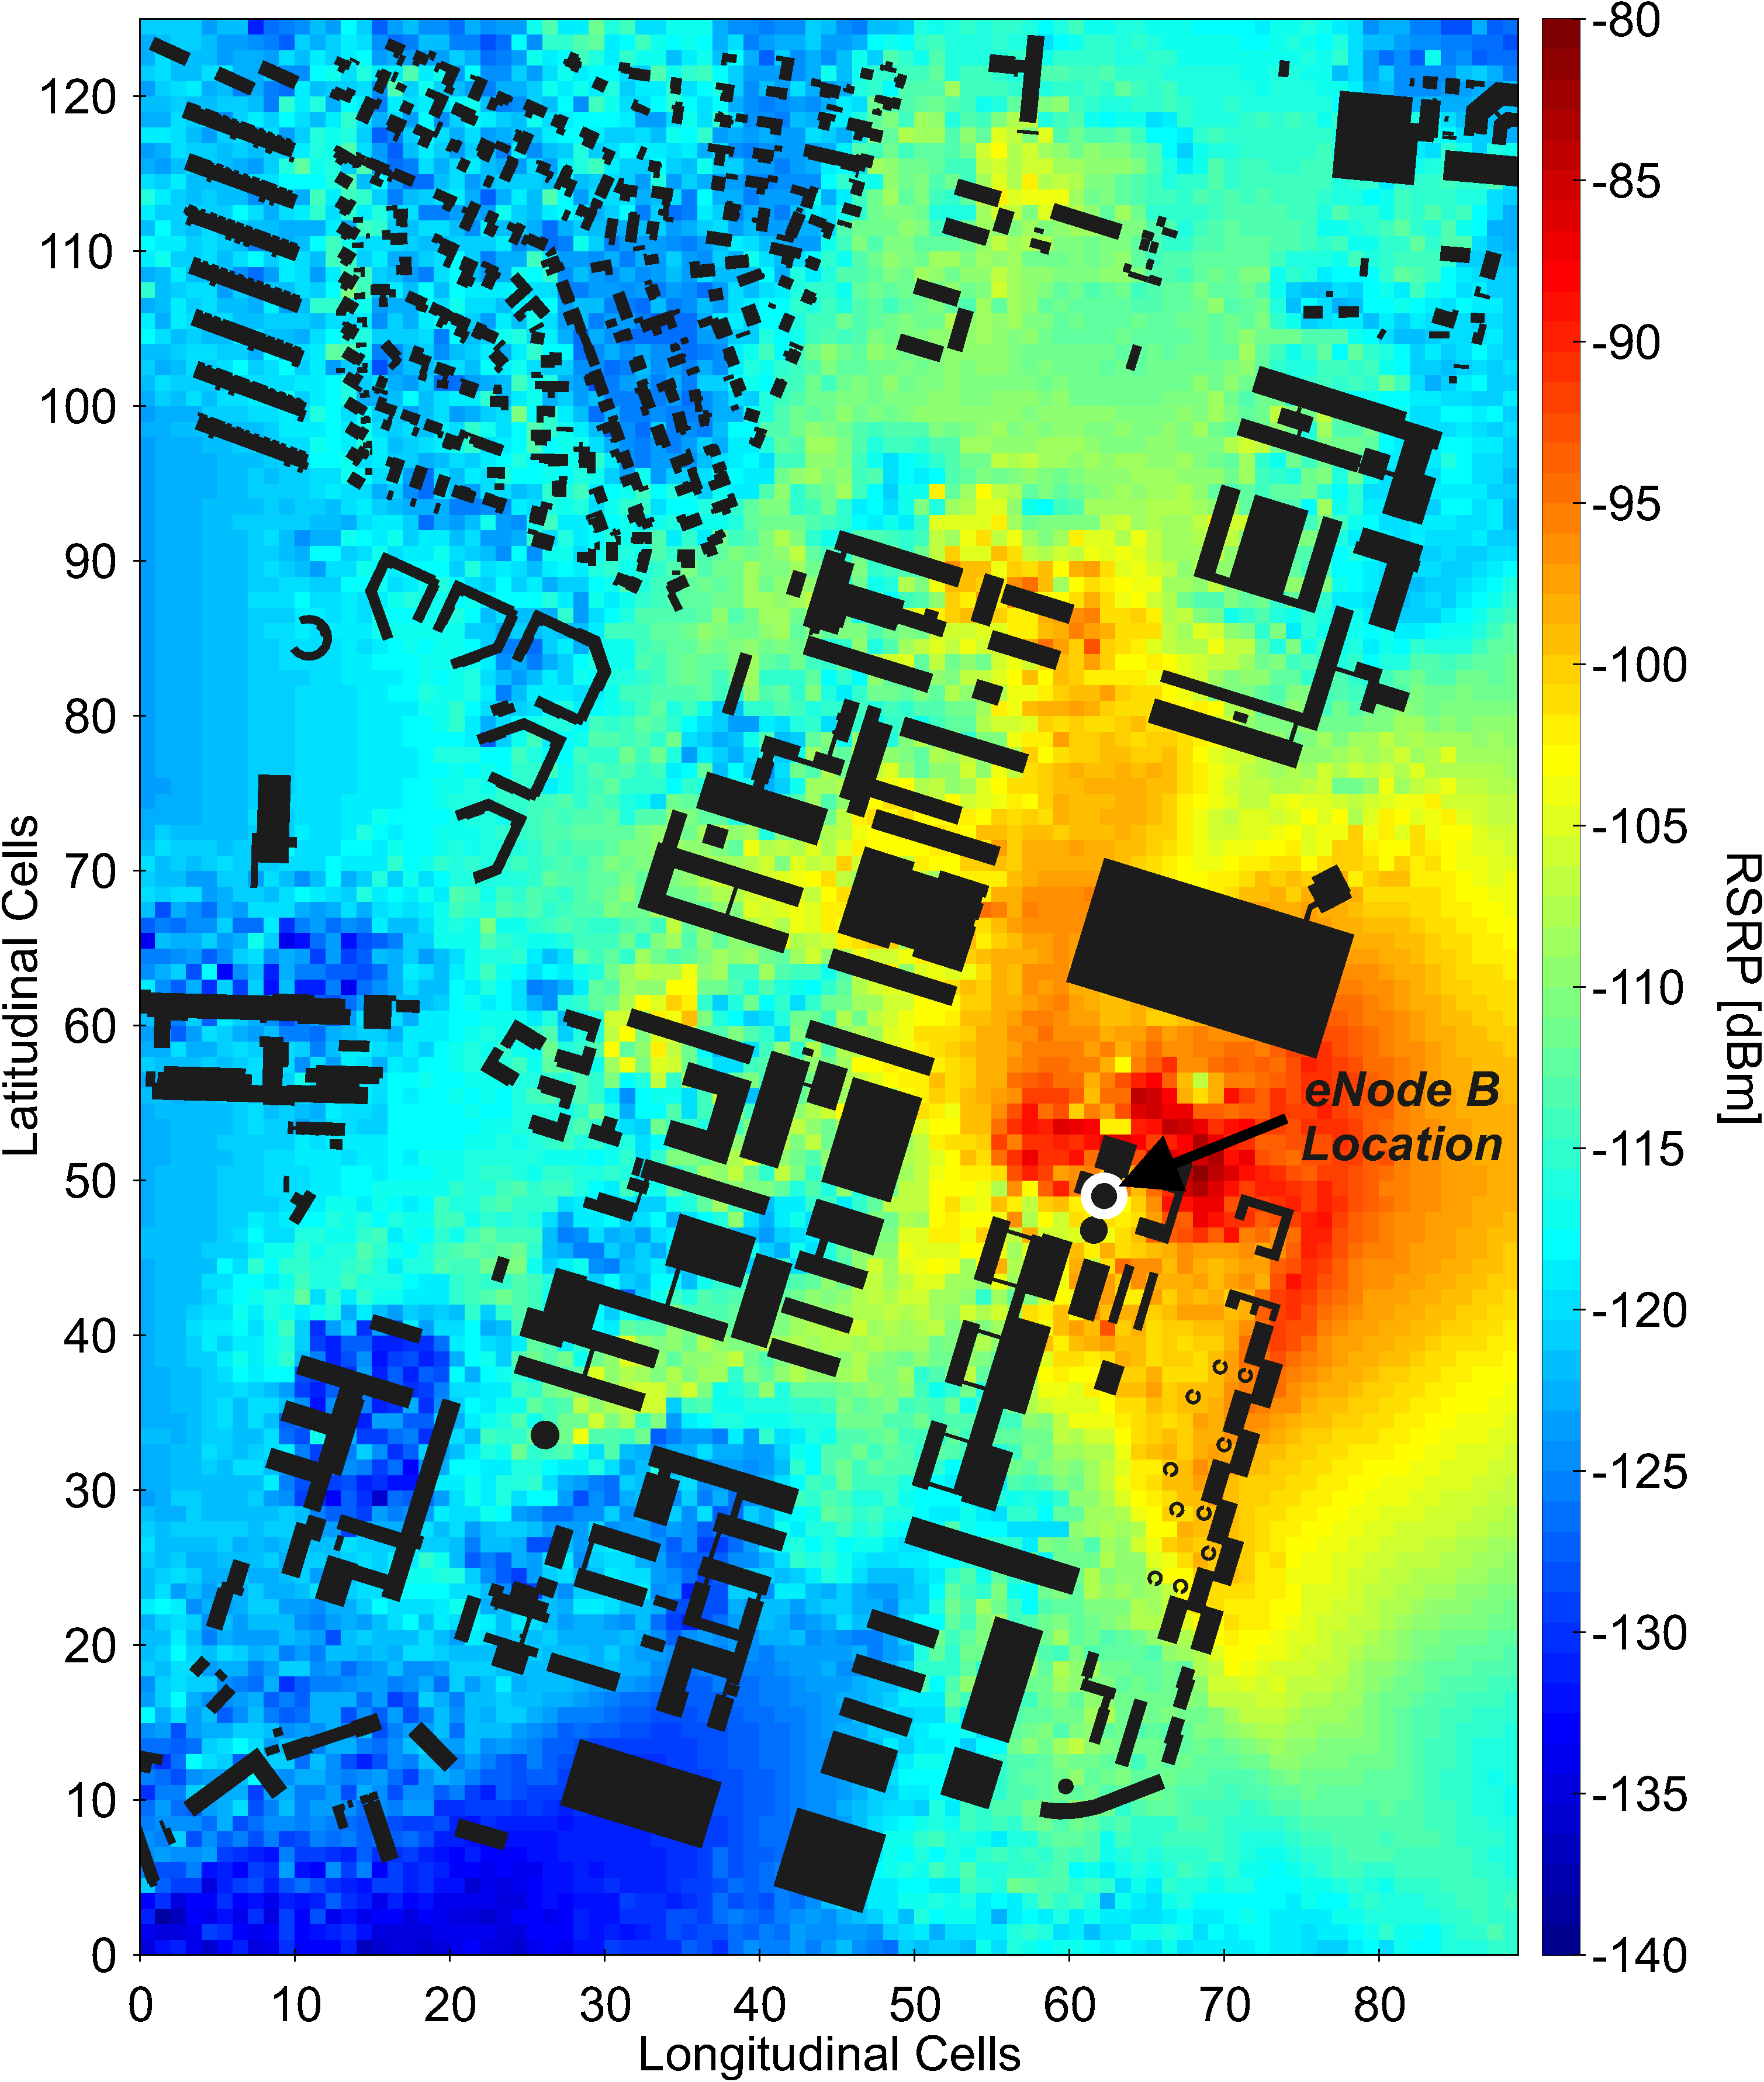
\includegraphics{chapters/part_pathloss/osm_images_paper/figures/heatmap.pdf}
    \caption{Extrapolated heatmap at 2630 MHz using generated features for all latitude and longitude coordinate pairs.}
    \label{fig:osm_heatmap}
\end{figure}

\subsection{Discussion}

A necessary procedure of the proposed method is experimental validation from inherently different data sources. The above-documented results contribute towards such a validation. The use of the German-based datasets is an essential first step in showing the properties and gains of the proposed method. The German-based datasets consist of several frequencies not present in the original \texttt{DK} dataset. More so, it effectively doubles the number of available samples for learning. The procedure for generating the geographical images is simplified as it only requires \gls{osm} data. 

The generalization performance has been analyzed using a cross-validation approach. A necessity of this approach is multiple trained models which is contingent on feasible training times. Evaluating the \texttt{DK Campus} subset is effectively extrapolation across data with an inherently different origin. The results indicate that the generalization across datasets with different data origin is possible and offer accurate performance $\text{\gls{rmse}} = 7.8$ dB. However, by including data from different origins the accuracy is effectively improve as is indicated by the performance $\text{\gls{rmse}} = 6.3$ dB of the \texttt{GER Campus} scenario. The  \texttt{GER Campus} is the campus of TU Dortmund, which does share many architectural similarities with the \texttt{DK Campus} scenario. The results indicate that this is inferred from data with a different origin. 

The geographical images supplied by a \gls{osm} pipeline have effectively resulted in a simplified training procedure and a significant reduction in hyper-parameters. Even with the reduction of hyper-parameters, the original reported gains (as seen in \emph{v2} and \cite{Thrane020ModelAidedDeepLearning}) on the \texttt{DK Campus} dataset are maintained. A direct result of this reduction is the main driver for the cross-validation procedure to be completed in a feasible time. The training time, with over double the amount of samples and a lower batch-size, is maintained at approximately $120$ minutes. The inference time is halved to sub-millisecond predictions.

The produced heatmap offers insight into the predictive capabilities of the method. Even though the heatmap is produced on the scenario at which it was trained, it still had to infer \gls{rsrp} for non-measured locations. The fact that the range of \gls{rsrp} values is within expected values is a favourable property of the trained \gls{nn}. Furthermore, the heatmap shows an increased intensity around the location of the \gls{enb}, which is probably. Finally, some sectorization of the \gls{enb} can, with some imagination, be observed. Future work of the methodology is not only to further test the generalization properties but also the performance to existing methods of producing radiomaps, for instance, compare the proposed approach to that of \emph{Kriging}.

% Altitude information embedding
Additionally, the images contain only information on the building footprints. It would be of great interest to study the embedding of altitude and height information into such images. 


\subsection{Conclusion}\label{subsec:conclusion_v3}
Simple geographical images, along with expert knowledge supply strong prior information for predicting \gls{rsrp} for unseen locations. It is shown that latent features for describing local radio characteristics can be found using simple geographical images. The proposed approach is vigorously validated on additional experimental data. The images were produced using a simplified pipeline utilizing \gls{osm} data and contain only information on buildings and the location. Images spanning a distance of $250-300$ meters was found to produce improved performance. The results show that the proposed method is able to generalize across inherently different data origins. The best predictive performance on an unseen propagation scenario is reported to be $\text{\gls{rmse}} = 6.3$ ($\sigma = 3.6$ dB) on a multitude of operating frequencies.





\section{Identified Challenges}\label{sec:identified_challenges_satellite}
A multitude of model architectures and training procedures have been documented throughout this Chapter. Along the way several pressing technical challenges have been identified. These can be reduced to the following items.

\begin{itemize}
    \item Convolutional layers are challenging to interpret.
    \item Embedding expert knowledge for other signal quality parameters.
    \item Clutter and Altitude/Height information not easily available.
\end{itemize}

The use of a \gls{cnn} for processing the images is a powerful tool for enabling latent features useful for signal quality parameter prediction. Essentially, \gls{cnn} use convolutional layers (or filterbanks) to apply a set of filters and feature extraction principles for reducing input images into useful features. In other words, the trained model consists thus of filters. The filters activate on important statistics present in the images, that are useful for the final predictors. Thus, in order to effectively improve the proposed methods, such filters needs to be further investigated and explored. However, such a testing and experimental procedure is not trivial and requires not only vigorous testing but also a significant number of samples for validating any resulting knowledge obtained. The addition of the German-based measurements enables such studies, therefor it is imperative for future studies that the learned filters are analysed.

It is shown that the model can be improved by embedding expert knowledge, in terms of a path loss model, into the training procedure. The results of the initial version (\emph{v1}) show that other signal quality parameters (such as \gls{rsrq} and \gls{sinr}) can be predicted with high accuracy. An identified challenge is the embedding of expert knowledge capable of aiding the prediction capabilities of such parameters. 

The use of simplified geographical images does not increase the prediction errors compared to utilizing high-resolution satellite images. In both cases no altitude or height information is embedded. Some height information are embedded in the satellite images, in terms of shadows of the resulting buildings and other details. However, as shown in state-of-the-art image segmentation algorithms, deducing building height from shadows alone is prone to significant errors. Thus, a challenge of the methodology would be to explore new avenues of embedding height information. In the \gls{osm} images, such a feature could be directly enabled onto building shapes by for instance using a color-mapping. Clutter data, important for higher frequencies (e.g. shorter wavelengths) is shown to have significant impact on the received power of the receiving devices. Thus being able to model such data is critical to accurate predictions. Therefor, extending the image information with clutter related data while keeping the data complexity low seems like a logical next step for the use of the methodology.


\section{Summary}\label{sec:satellite_image_discussion}
The process of utilizing satellite images for path loss prediction has been an ongoing process of relevant study items. The different iterative steps for improving and studying the approach has been documented throughout this chapter, an termed by the different \emph{versions}. The outcome of each iteration has extensively been discussed and can be summarized as follow:
\begin{itemize}
    \item \emph{Version 1} Initial exploration - Proof of concept. Generalization issues and further need for comparative studies.
    \item \emph{Version 2} Model-aided approach - Applied techniques for improving generalization and the comparison to traditional approaches.
    \item \emph{Version 3} Simplified images - Additional measurements from an inherently different origin. The study of simplistic images and the impact on predictive performance
\end{itemize}

\textcolor{red}{Maybe add figure here if time allows it}


The iterative improvements of the model has allowed for well-defined conclusions. Taking a step back, the knowledge obtained can be reduced for relevant terms associated with wireless communication and cellular networks. It was well known in literature that \gls{nn} can provide with highly accurate path loss predictions that can (possibly) assist in deployment and optimization processes of the cellular networks. However, what is not discussed is the underlying dangers of supervised learning. It can be seen throughout \emph{version 1} and also to some extent \emph{version 2} that high performance can be achieved on the dataset at which the model is trained. Which is obvious due to the fundamental principles of \gls{ml}. The dangers of supervised learning arise when the generalization is unexplored or with significant bias. This is explore and testing in \emph{version 3} by using a inherently different data source. If \gls{nn}-based path loss models are to be of any use, vigorous testing and comparative studies are essential otherwise such models are useless. The aim of the method developed throughout this PhD project has been to go beyond that and lay the foundation for methods that not only improve performance in terms of dB but also ensure the predictions are within reason and intuition. 

Much more data can essentially be integrated into path loss modelling using the principles documented throughout chapter. It is important that the complexity of such that (not only obtaining it but also processing it) remains low otherwise the models become useless for their sole purpose: \emph{To model capacity and coverage for the optimization of cellular systems and infrastructure.}
\chapter{The unforgiving LOS-state}\label{ch:deepindoor}
The task of predicting attenuation of radio transmission in \gls{o2o} scenarios increases in complexity with increased distance, due to the increased number of objects in the radio environment. The task of predicting attenuation in \gls{o2i} is significantly more complex, due to specific interactions of the different materials in between the transmitter and receiver antennas. The campus of The Technical University of Denmark (DTU) consists of a unique underground system. Given the efforts spent in understanding and applying Deep Learning to path loss estimation for \gls{o2o} scenarios, utilizing this unique tunnel system for studies seemed relevant for improving and evaluating current models available in literature. This has resulted in to publications

\begin{itemize}
    \item \textbf{Investigation of deep indoor NB-IoT propagation attenuation}, IEEE VTC-Fall 2019 \cite{Malarski2019InvestigationAttenuation}
    \item \textbf{Experimental Evaluation of Empirical NB-IoT Propagation Modelling in a Deep-Indoor Scenario}, submitted for Globecom 2020 \cite{Thrane2020ExperimentalScenario}
\end{itemize}

The former introducing the concepts of Deep Indoor propagation modelling with an initial measurement study. This was extended in the latter work, with an extensive measurement campaign utilizing complex LIDAR data to offer accurate positions and features. The latter is furthermore the foundation for the majority of the content throughout this chapter. 

\section{Deep Indoor}

With the development and standardization of \gls{lpwan} technologies such as \gls{nbiot} battery powered sensors are being deployed in unreachable scenarios (usually indoor) to allow for new application and services \cite{Sinha2017ANB-IoT}. This will result in a significant number of complex deployment situations where an accurate coverage model is a necessity \cite{Lauridsen2016CoverageArea}. In the case of indoor deployments where already deployed 4G, \gls{lte} or 5G, \gls{nr} basestations are utilized for transmission we term the transmission scenario as \gls{o2i}. A comprehensive introduction and summary of the inner workings and best practices for deploying \gls{nbiot} can be found in references such as \cite{Sinha2017ANB-IoT, Li2018SmartNB-IoT, Chen2017NarrowThings} and references herein.

The applications of \gls{nbiot} are many due to the long-range transmission qualities, and the battery operated sensors. The application of \gls{nbiot} to remote monitoring is subject to reliability concerns regarding 1) reliably connectivity and 2) regulated power consumption. For instance, placing sensors in hard to reach areas, such as used for smart water metering it is essential that the sensors are reliable and not subject to repair or replacement within short periods of deployment \cite{Popli2019AChallenges}. 



\begin{figure*}
    \centering
    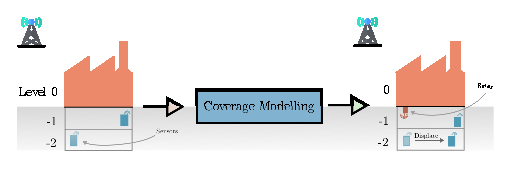
\includegraphics{chapters/part_pathloss/figures/outdoor_to_indoor/approach_figure.eps}
    \caption{Deployment of sensors in deep indoor situations may require displacement or added relays to ensure the desired connection reliability.}
    \label{fig:outdoor_to_indoor_approach}
\end{figure*}

Coverage modelling is an essential element for deploying any \gls{nbiot} sensor, and an even more important aspect when deploying sensors in hard to reach areas. This is the case from both the perspective of the \gls{mno}, but also the cosumer and enterprise owning the sensors. For instance, as visualized in Fig. \ref{fig:outdoor_to_indoor_approach} some sensors might require displacement to ensure reliable connection, and in some cases it might even be necessary to deploy local relays. Both of which require expensive trial-and-error experiments if no accurate coverage modelling can be applied.  

\subsection{Outdoor-To-Indoor empirical models}
Both \gls{3gpp} and \gls{itu} have in the latest technical reports, concerning coverage models and path loss estimation, supplied with so-called \gls{o2i} models. The models provide with terms for attenuation associated with 1) penetration losses and 2) the distance inside the building. The documents are focused on indoor scenarios related to regular buildings. E.g. distances indoor define the distance to the outer most wall that seperates the receiver antenna from the transmitter antenna. More specifically, the losses are decomposed as followings

\begin{equation}\label{eq:o2i_pl}
    PL_{O2I} = PL_{b} + PL_{tw} + PL_{in}
\end{equation}

Where $PL_{b}$ is the basic outdoor path loss as denoted by the \uma{A} and \uma{B} models as described in Section \ref{sec:empirical_path_loss}. The terms, $PL_{tw}$ and $PL_{in}$ are losses associated with building penetration and the distance indoor respectively. The losses associated with the penetration, are composed into a low-loss and high-loss model, both being frequency dependent, but constant with distance.  On the other hand losses related to indoor distance ($PL_{in}$) are dependent on an indoor distance parameter as follows

\begin{equation}\label{eq:o2i_pl_in}
    PL_{in} = 0.5 \cdot d_{in,2d}
\end{equation}

Where $d_{in,2d}$ denotes the distance indoor, i.e. the distance to the outer most wall in the direction of the transmitter. The entirety of Eq. (\ref{eq:o2i_pl}) are undefined for indoor scenarios different from level 0, 1 and 2. Furthermore, the indoor distance metrics are unspecified for underground positions. 

The remainder of this chapter contains an experimental investigation for deep indoor path loss modelling. More specifically, evaluating current models and the performance for scenarios that are different than regular buildings, i.e. \gls{o2i} where the indoor attenuation is partially underground. 

\subsection{Deep Indoor attenuation}
Radio propagation modelling for tunnels have been subject to significant research due to the many radio applications residing in tunnels. For instance, railway operators require reliable communication networks to ensure safety and effective maintenance. A comprehensive survey of radio propagation modeling for tunnels can be found in \cite{Hrovat2014ATunnels}. The paper discuss the use of ray-tracing models and empirical models (among others) and the resulting predictive accuracy. It is found that the geometry of the tunnel system, especially the cross-sectional shape is significantly important for estimation of radio propagation. It is found that ray-tracing models that utilize such cross-sectional geometry information perform better in both NLOS and LOS situations. However, this is not the case for empirical models that are found to be lackluster in predictive performance when predicting the NLOS state. Finally, it should be said that the scope of the research generally considers transmission within tunnel systems. In other words, the unreliable transmission characteristics of \gls{o2i} pushes mobile operators to install relays and base stations inside the tunnel systems making radio propagation models inside tunnels important. The purpose of the study is not to enrich literature with improved empirical models for radio propagation in tunnel systems. It is however the objective to investigate how current empirical models preform for \gls{nbiot} technologies in a \gls{o2i} transmission scenario.

\section{Deep Indoor Measurements}
Getting positions indoor is not a trivial task, as common solutions using \gls{gnss} are unavailable. Techniques for inferring positions indoor using radio waves with high accuracy have been documented in literature \cite{Nuaimi2011}, however, such solutions require complicated infrastructure and post-processing. In this particular case, the unique tunnel system is scanned using high-resolution LIDAR. The availability of such data enables accurate indoor positioning, and advanced feature engineering for investigating indoor attenuation and parameters related hereof.  Initial evaluations of deep indoor attenuation were completed in \cite{Malarski2019InvestigationAttenuation}, using a simplistic metric of indoor distance. It shows a inaccuracy of using $PL_{in}$ in deep indoor scenarios, but is subject to additional measurements and research. The availability of the LIDAR data increases the accuracy of the study and the resulting indoor distance features. 


\subsection{Tunnel system}
The tunnels span the entirety of the Technical University of Denmark campus providing a unique location for long-distance deep indoor measurements. The layout, and the measurements conducted are visualized in Fig. \ref{fig:underground_tunnel_system}.

\begin{figure}
    \centering
    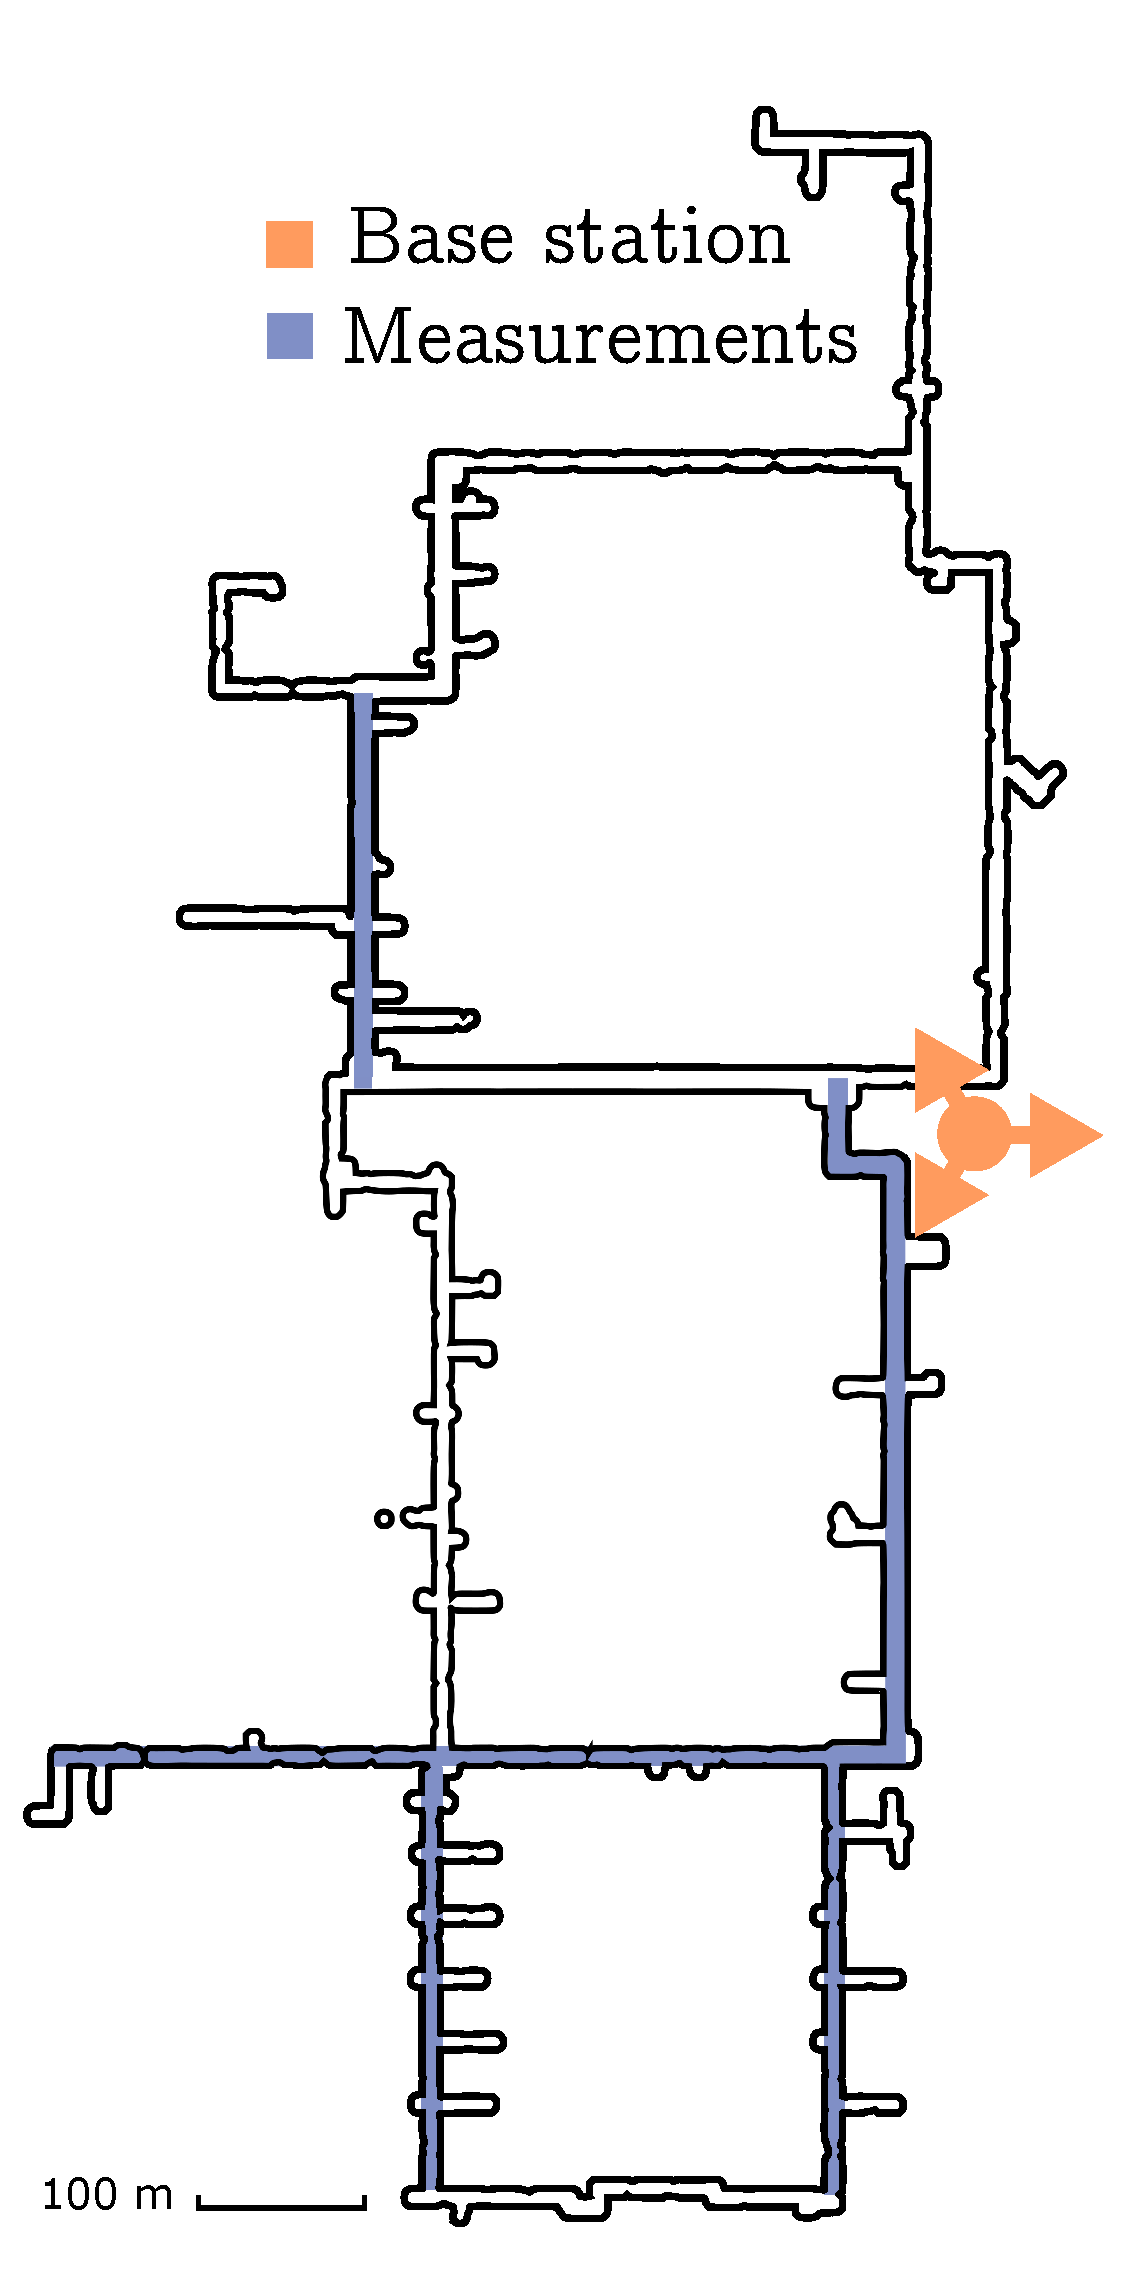
\includegraphics[width=0.5\textwidth]{chapters/part_pathloss/figures/outdoor_to_indoor/Complete_tunnel_system.eps}
    \caption{The underground tunnels of The Technical University of Denmark campus. The areas of measurements are highlighted.}
    \label{fig:underground_tunnel_system}
\end{figure}



\subsection{LIDAR}
A complete LIDAR scan of the tunnel system have been conducted with a very granular resolution of $> 1$ cm. The LIDAR data provides with a set of $3$D coordinates $(x_i, y_i, z_i)$ for the entirety of the tunnel system. Accumulating to $\approx 20$ GB of files, with approximately $100$ million coordinate pairs. Custom LIDAR scripts have been written to process the data. The was largely enabled by libraries such as LasPy \cite{Grantbrown/laspy:1.0-1.4.} for LIDAR file processing, and \cite{alan_d_snow_2020_3714221} for coordinate conversion. Examples of the point cloud, and the data can be seen in Fig. \ref{fig:tunnel_cross_section} and Fig. \ref{fig:tunnel_3d_view}.

\begin{figure*}
    \centering
    \caption{Cross-sections of a tunnel corridor on the xz-plane. Details of pipes, ventilation and other indoor features are visible.}\label{fig:tunnel_cross_section}
    \subfloat[]{\includegraphics[width=0.3\textwidth]{chapters/part_pathloss/figures/outdoor_to_indoor/crossection_1.png}}
    \subfloat[]{\includegraphics[width=0.3\textwidth]{chapters/part_pathloss/figures/outdoor_to_indoor/crossection_2.png}}
    \subfloat[]{\includegraphics[width=0.3\textwidth]{chapters/part_pathloss/figures/outdoor_to_indoor/crossection_3.png}}
    \vspace{2em}
\end{figure*}

The LIDAR coordinate pairs are given in a coordinate systems related to that of the DTU campus termed DTULOK. A procedure for converting to the UTM32 system is provided along with the dataset, consisting of a so-called Helmert transformation. 


\begin{figure}
    \centering
    \includegraphics[width=\textwidth]{chapters/part_pathloss/figures/outdoor_to_indoor/3d_view.png}
    \caption{$3$D view of the LIDAR pointcloud limited on the Z-axis to show a horizontal cross-section.}
    \label{fig:tunnel_3d_view}
\end{figure}


\subsection{Setup}

\begin{table}[htbp]
\centering
\begin{tabular}{@{}l|l@{}}
\toprule
\# of measurement points       & $895$             \\ \midrule
TSMW/UE measurements per point & $1e6/10$          \\ \midrule
Operating frequency            & $820.5$ MHz       \\ \midrule
Bandwidth                      & $180$ kHz         \\ \midrule
Noise figure (TX/RX)           & $5$ dB/$3$ dB     \\ \midrule
TX power                       & $46$ dBm          \\ \midrule
Receiver antenna position      & Vertical          \\ \midrule
TX/RX antenna gain             & $5$ dBi/$5.8$ dBi \\ \bottomrule
\end{tabular}
\caption{Measurement configuration and parameters}\label{tab:measurement_configuration}
\end{table}

The setup consists of a \gls{r_and_s} TSMW Network Tester \cite{Manual2017} (as also utilized for drive-testing, see Appendix \ref{app:drive_test_study_2017} and \ref{app_drive_test_study_2020}). And a \gls{nbiot} device \cite{sodaq}. Antennas for both the TSMW, and the \gls{nbiot} device was mounted vertically on a trolley. Utilizing a laptop with a set of parallel measurement scripts, measurements from both the TSMW and \gls{nbiot} device were conducted for each measurement position. More specifically, a measurement was taken with constant intervals for individual corridors. This results in $N$ measurements for each corridor, ideally equidistant spaced with $1$ to $2$ m. For each decided measurement position, the following measurements were taken

\begin{itemize}
    \item $1e6$ \gls{iq} samples (TSMW)
    \item $10$ \gls{rsrp} Measurements distributed over $20$ seconds (\gls{nbiot} device)
\end{itemize}


The \gls{iq} samples were taken utilizing a low-pass filter centered around the \gls{nbiot} operating carrier frequency given the bandwidth of a single narrowband of $180$ kHz. An overview can be found in Table \ref{tab:measurement_configuration}. 

The \gls{rsrp} measured was averaged over all samples taken at each measurement position to average out any time-variant impairments that may have influenced the \gls{rsrp} at time of measurements.. 



\subsection{Indoor positioning}
In order to utilize the LIDAR scan for indoor positioning, a procedure was developed. It can be summarized as the following step-wise procedure. It consists of the following steps:

\begin{enumerate}
    \item Identify start and end positions of measurement campaigns within the $3$D point cloud.
    \item Interpolate measurement positions ($x, y$) given the start and end positions and the number $N$ measurements conducted.
    \item Look-up the interpolated coordinates to obtain ($x, y, z$) pairs.
    \item Convert local coordinate system (DTULOK) to UTM32/WSG84
\end{enumerate}

Accurate identification of the start and end positions within the point cloud (step 1) is paramount to high accuracy for the remainder of the measurement positions. In order to achieve accurate identification, the step was split into two procedures, a) ensuring the start and end positions was well documented with pictures and can visually be identified using e.g. a large pipe or other significant characteristics of the environment. b) an interactive program was created to narrow down such characteristics within the point cloud. An example can be seen on Fig. \ref{fig:tunnel_3d_view}. 

The interpolation (step 2) assumes equidistant measurements. It is fair to assume some errors may introduce themselves during the measurements, however, by ensuring the total distance between the start and end position is divided into $N$ segments, the overall equidistant error is averaged out.

The look-up of coordinates (step 3) consisted of computing the distance (euclidean) to LIDAR coordinate pairs. The closest point within the point cloud was then extracted as the coordinate. Due to the high resolution, on average the closest point was within a margin of $1$ cm.

The LIDAR data operates within a coordinate system localized to the area of measurements. A conversion (step 4)  to more generic coordinate systems such as UTM32 and WSG84 (Latitude, Longitude) \cite{alan_d_snow_2020_3714221} completed the indoor positioning procedure. 


\section{Evaluation of indoor KPIs}
The literature for indoor attenuation states that 1) tunnel geometry is considered the main influence on attenuation for propagation in tunnels, and 2) current models for \gls{o2i} use a simple indoor distance metric. Having access to the high resolution LIDAR data enables the engineering for indoor distance metrics with high accuracy. 


\subsection{Feature Engineering}
The bearing between the receiving and transmitting antenna (also known as the azimuth angle $\phi$) can be determined by the WGS$84$ coordinates of the measurement position and the transmitting antenna. Additionally, the altitude information provided by the LIDAR data, offers means for computing the elevation angles (the height of the transmitter is known). Thus, the accurate indoor position in $3$D enables simple computation of the azimuth ($\phi$) and elevation ($\theta$) angles. Furthermore, this in combination with the LIDAR data enables distance calculations in both $2$D and $3$D space. 

In order to be capable of computing the require indoor distance metrics, a few requirements are needed. Firstly, the tunnel geometry must be quantified such that distances can be computed to intersecting tunnel walls and edges. Secondly, height of the terrain must be know, at points in space where the "straight-as-the-crow-flies" path to and from the transmitting antenna intersects with the terrain. Formalizing the tunnel geometry was done by inspecting the LIDAR data and designing so-called boundary boxes in $3$D space. Thus, the boundary boxes determine the geometry of the measured tunnel for a given set of measurements. By doing so, and applying trigonometry, the following set of distance metrics in $3$D space was derived.

\begin{itemize}
    \item Indoor distance to the intersecting tunnel wall/edge $d_{in}$.
    \item Penetration distance, distance between the tunnel wall/edge and the terrain $d_{pen}$.
    \item Average $2$D distance to intersecting corridor $d_{cor,avg}$
\end{itemize}


\begin{figure}
    \centering
    \includegraphics{chapters/part_pathloss/figures/outdoor_to_indoor/inside_distance_illustration.eps}
    \caption{Distance metrics utilizing tunnel geometry and accurate indoor positions using elevation angles $\theta$}
    \label{fig:inside_distance_xz}
\end{figure}

\begin{figure}
    \centering
    \includegraphics{chapters/part_pathloss/figures/outdoor_to_indoor/inside_distance_illustration_xyplane.eps}
    \caption{Distance metrics utilizing tunnel geometry and accurate indoor positions using azimuth angles $\phi$}
    \label{fig:inside_distance_xy}
\end{figure}

\noindent A few edge cases arose when using the engineered boundary boxes of the tunnel geometry. Firstly, a set of measurements were almost directly below that of the transmitter (as seen by Fig. \ref{fig:underground_tunnel_system}). This resulted in a set of elevation angles, where the tunnel edge/wall was not the correct intersection between the "straight-as-the-crow-flies" path and the tunnel geometry. Instead, the roofing of the tunnel was the \emph{entry} point of the direct path. This required a re-computation of the distance metrics using a more advanced $3$D trigonometry approach. 

Secondly, some parts of the corridors consisted of several intersecting corridors. This meant that the distance to the tunnel edge/wall became dependent on a non-rectangular boundary box covering the tunnel measured. Such a boundary box is time-consuming and exhaustive to create in $3$D space. However, by doing so the engineering of the feature $d_{cor,avg}$ was enabled using unique identifers for each intersecting tunnel across the system.

Finally, the terrain information for computing and deriving the penetration distance did not include any buildings. A so-called \gls{dtm} \cite{kortforsyningen} was utilized for extracting altitude information, effectively providing an accurate approximation of the terrain covering the area of the underground tunnel system.


\subsection{Results}

\begin{table}
    \centering
    \begin{tabular}{@{}l|ll@{}}
    \toprule
    Regressors               & $R^2$ & Residual MSE \\ \midrule
    $3$D distance              & $0.285$ & $74.973$       \\
    $d_{in,2D}$              & $\mathbf{0.026}$ & $\mathbf{102.098}$      \\
    $d_{in,3D}$              & $0.026$ & $102.097$      \\
    $d_{pen,3D}$             & $0.017$ & $103.022$      \\
    $d_{pen,3D} + d_{in,2D}$ & $0.005$ & $104.335$      \\
    $d_{cor,avg}$            & $\mathbf{0.148}$ & $\mathbf{89.286}$       \\
    $d_{pen,3D} + d_{in,2D}+d_{cor,avg}$ & $0.150$ & $89.276$       \\
    $d_{pen,3D} + d_{in,3D}+d_{cor,avg}$ & $0.150$ & $89.276$       \\
    $\phi + \theta$          & $\mathbf{0.173}$ & $\mathbf{86.763}$       \\ \bottomrule
    \end{tabular}
    \caption{Results of linear regression using OLS \cite{seabold2010statsmodels}}\label{tab:ols_results}
    \vspace{1em}
\end{table}
\noindent The measured \gls{rsrp} concatenated for all measurement subsets (i.e. corridors) are seen in Fig. \ref{fig:indoor_distance_reg} as a function of the $3$D distance (a), and $d_{in,2d}$ (b). Also shown is the prediction of the basic path loss offered by the \gls{3gpp} \gls{uma} model as given by partly by Eq. (\ref{eq:uma_nlos_pathloss_max}). The full path loss model can be found in \cite{38211}. Several (easy separately) clusters are observed for \gls{rsrp} as a function of $d_{in,2d}$, as seen in Fig. \ref{fig:indoor_distance_reg}(b), corresponding to each of the different corridors in which measurements were conducted.

\begin{figure}
    \centering

    \subfloat[Theoretical path loss model vs \gls{rsrp} measurements]{\includegraphics[width=0.8\textwidth]{chapters/part_pathloss/figures/outdoor_to_indoor/results/d3d_rsrp_3gpp.eps}}
    \\
    \subfloat[Indoor distance]{\includegraphics[width=0.8\textwidth]{chapters/part_pathloss/figures/outdoor_to_indoor/results/d2d_wall_rsrp.eps}}
    
    \caption{The prediction provided by the theoretical path loss model $PL_b$ in Eq. (\ref{eq:o2i_pl}) is shown in (a). The indoor distance for all measurements in shown in (b).}\label{fig:indoor_distance_reg}

\end{figure}

The results of a linear regression using \gls{ols} are observed in Table. \ref{tab:ols_results}. The inner workings of the \gls{ols} method are further described in \cite{seabold2010statsmodels}. Briefly summarized it consists of minimizing the sum-of-squares (as is given by Eq. (\ref{eq:sum-of-squares}) using a simple linear model formulation of roughly $y=ax+b$ with the objective to find $a$ and $b$ (a more refined definition can be found in \cite{M.Bishop2006}). 

The results of the linear regression shows a correlation coefficient $R^2$ of $0.026$, with a residual \gls{mse} of $102.098$ using the indoor distance metric of $d_{in,2d}$. Adding and using the elevation angle to obtain $d_{in,3d}$ offers no increase or decrease in the linear model performance. The use of $d_{pen}$ in $3$D have a decrease in  $R^2$ of $\approx 0.001$ compared to the metric of $d_{in}$, and an increase in the residual \gls{mse} of $\approx 1$ dB. Most noticeably is the increase in linear predictive performance when using the parameter $d_{cor,avg}$, and furthermore when utilizing the azimuth and elevation angles $\phi, \theta$.


The predictive performance of utilizing the \gls{o2i} path loss model given by Eq. (\ref{eq:o2i_pl}) is shown in Fig. \ref{fig:mae_boxplot_o2i_pl_in}. The indoor distance parameter of Eq. (\ref{eq:o2i_pl_in}) is altered to use the engineered features of indoor distance, and penetration distance, and a combination of. In other words, the parameter of $d_{in}$ is substituted with the engineered distance features. The \emph{none} case is the use of Eq. (\ref{eq:o2i_pl}) but without the term of $PL_{in}$. It can be seen that the average predictive error of $9.9$ dB is achieved using no terms for attenuation related to indoor distances. A decrease in predictive performance, e.g. an increase in \gls{mae} of $\approx 1.1$ dB is observed utilizing $d_{in,2d}$ as an indoor distance parameter. The performance decreases as the remainder of the engineered features are utilized, peaking at $\approx 26.9$ dB of error using $d_{in,3d}+d_{pen,3d}$ as the indoor distance metric. Finally, it can be said that the performance generally decrease with an increase in distance indoor distance utilizing the proposed model of Eq. (\ref{eq:o2i_pl}).

\begin{figure}
    \centering
    \includegraphics{chapters/part_pathloss/figures/outdoor_to_indoor/results/mae_boxplot.eps}
    \caption{\gls{mae} predictive \gls{rsrp} performance utilizing Eq. (\ref{eq:o2i_pl}) using different indoor distance parameters.}
    \label{fig:mae_boxplot_o2i_pl_in}
\end{figure}

\subsection{Discussion}
The additional path loss based on indoor distance does not in the current state reflect that of Deep-indoor situations. The model of estimating loss associated indoor with indoor distance offer an increase in predictive error of \gls{rsrp} as the indoor distance increase. This is caused by 1) the losses associated with penetration (i.e. $PL_{tw}$) does not reflect the mean attenuation satisfactory, and 2) the model uses a constant term that is distance based. As highlighted by the results of the linear regresssion, using any of the indoor distance metrics of $d_pen$ or $d_in$ is a poor choice of a predictor using a linear model than compared to 1) features of tunnel geometry $d_{cor,avg}$, and 2) angles of azimuth and elevation. From these findings it indicates that A) tunnel geometry-based features are superior to indoor distance features and B) The geo-statistics of the measurement area is complex and thus \gls{rsrp} is highly dependent on local variability. In summary, the findings of A) highlights the importance of tunnel geometry in \gls{o2i} propagation scenarios, and B) Attenuation is largely based on localization, which indicates complex local variability terms.

The engineering of such indoor features of $d_{pen}$ and $d_{in}$ is not a trivial task for underground tunnel systems. Regardless of the features having reduced importance for \gls{rsrp}, obtaining such features is a challenge and is furthermore not suited for use in empirical path loss models. The proposed empirical models should maintain a set of features that are feasible to obtain to motivate the purpose of such models. In this particular case of a tunnel system, the use of any indoor distance metrics to outer wall can be computed using the accurate LIDAR data. However, this is considered a unique data source and is not a common practice in most deep-indoor scenarios. In other words, the attenuation term based on indoor distance provided by Eq. (\ref{eq:o2i_pl_in}) is not only a poor model for tunnel systems, it also requires a feature that in most cases is a challenge to obtain. Instead, and as indicated by the results, local features of tunnel geometry may offer improved predictive performance, and fewer challenges in terms of engineering the required data. For instance, measuring any distance inside of the tunnel can simply be done with measuring tape and requires no features of accurate indoor position or complex tunnel geometry data. Finally, it is indicated by the results that any empirical model capable of offering satisfactory predictions in such a deep-indoor situation must consider two essential terms for attenuation 1) the distance to the transmitter and 2) extra attenuation terms based on localized tunnel geometry. The remainder is set as future work for the obtained set of measurements.

\subsection{Conclusion }

A comprehensive procedure for obtaining accurate indoor positioning using LIDAR data was developed along with a completed measurement campaign for \gls{nbiot} \gls{rsrp} values. The LIDAR data enabled the engineering of indoor distance parameters for using in existing empirical \gls{o2i} path loss models. A statistical analysis utilizing linear models shows a poor performance reflected by such indoor distance parameters. Instead, features related to localization (angles) and tunnel geometry (average distance to intersecting corridors) shows improved importance for predicting \gls{rsrp}. This was furthermore validated when substituting the engineered indoor distance metrics into existing empirical path loss models for indoor attenuation. Removing the term for indoor attenuation from the \gls{o2i} path loss model offered improved predictive results (of $1.1$ to $26$ dB \gls{mae}). Finally, additional efforts should be spent towards engineering features in deep-indoor scenarios representing local tunnel geometry that are first and foremost feasible to obtain. 

\section{Deep Learning}

The above introduced and discussed project of path loss prediction in deep-indoor scenarios is considered unfinished and have a few near-future relevant milestones. Most noticeably, such milestones are related in areas of feature engineered. This, as seen from Chapter \ref{ch:satelliteImages}, is an area where tools from \gls{dl} thrive however with a few caveats and requirements. This section will seek to elaborate on possible applications of \gls{dl} within the area of feature engineering for deep-indoor propagation scenarios.

\paragraph{Data quantity}

Achieving the data quantity required for the application of \gls{dl} methods for automatic feature engineering is a significant draw-back. The LIDAR data might seem like an obvious choice for feature engineered, but it is ultimately limited by the measurements conducted. The discrete measurement procedure of equidistant measurement positions is a requirement for accurate indoor positioning, but limits the amount of measurements done. Thus, if a measurement procedure can be established that 1) enables continouous measurements (like common drive-testing practices) and 2) ensures accurate indoor positioning. The data quantity requirements for utilizing \gls{dl} can be satisfied. 

\paragraph{Formalization of raw data}
The LIDAR data seems useful as a source of raw data containing the necessary tunnel geometry information. However, it may to some extend contain too many data points for feasible runtimes and processing. Efforts of manipulating the data to be applicable for processing within tools of \gls{dl} is a necessary step for further model formalization. In some sense, the idea behind the utilization of satellite images could be transferred to deep-indoor situations. For instance, if the LIDAR data could be engineered in such a way that would embed the main characteristics of the tunnel system and allow for processing with convolutional layers. It could provide with a pipeline of adaptive filters that possibly can be used to infer and identify features of importance. This could then be utilized in future path loss models and thus relevant for empirical models and future studies. 


\section{Identified Challenges}
In this chapter the predictive performance of \gls{o2i} empirical path loss models in a deep-indoor propagation scenario have been evaluated for different indoor distance parameters. A procedure of deriving accurate indoor distance parameter have been presented and consequently discussed. Challenges of utilizing empirical models in deep-indoor propagation scenario, and the necessary steps required, have been identified and can be summarized as follows:

\begin{itemize}
    \item Indoor/underground distance parameters in underground tunnel systems is not trivial to engineer.
    \item Indoor attenuation terms for current empirical models (\gls{3gpp} $38901$ UMa) needs to be reevaluated for underground systems.
    \item Tunnel characteristics and geometry remains difficult to formalize for use in path loss estimation.
    \item A Deep Learning-based application is limited by data quantities regulated by the necessary steps for achieving accurate indoor positions.
\end{itemize}


\section{Summary}
The procedure of obtaining radio measurements with accurate indoor positions for the tunnel system at The Technical University of Denmark have consisted of two  distinct iterations. In \cite{Malarski2019InvestigationAttenuation}, a simple indoor position was derived using laser scanners providing with difference in x and y space. This approach translated poorly to long tunnels and required a difference procedure. This procedure is the majority of content in this chapter, and as presented in \cite{Thrane2020ExperimentalScenario}. Specifically, the outcome of the above detailed research can be reduced to the concrete following items

\begin{itemize}
    \item Current empirical path loss models offer poor performance in deep-indoor scenarios for \gls{nbiot}.
    \item Local tunnel features are more important for the prediction of received power than indoor/underground distances.
    \item Deep Learning may be able to engineer relevant features, but require significant work in formalizing the required data.
\end{itemize}

\chapter{Deep Learning for Radio Propagation Modelling}\label{ch:dl_radio_summary}
Radio propagation modelling is a difficult and complex task. The purpose of a radio propagation model is to provide the most accurate estimations of signal quality metrics. But as seen throughout this chapter, selecting the right model is a complicated procedure for any mobile communication system. The supposedly performance increase provided by highly detailed ray-tracing models is in any case expected to outperform simple empirical models. However, as seen in in chapter \ref{ch:channelmodellingbasics} this is not necessarily the case. Empirical path loss models are known and have been shown to offer a simple and effective model for approximating received power in mobile communication system. This, with additional statistics on large-scale fading phenomenon offer useful margins for use in the simplest of link-budget analysis and overall communication system design. 

The data complexity associated with the use of empirical models reduce the need for any complex data engineering. This is not the case for ray-tracing solutions. In Chapter \ref{ch:satelliteImages} a novel \gls{dl} method for estimating received signal \glspl{kpi} for use in mobile communication systems have been presented. The method is shown to be capable of utilizing different geographical images and features with overall low data engineering complexity and be capable of improving predictions for unseen locations. Doing so while keeping a low generalization error across different regions and data sources. Not only does this ensure a simple pipeline for estimating signal metrics it also ensures that the method is sufficiently simple to use. This is a key property and enables the many applications that have made traditional empirical models incredibly useful. For instance, in greenfield deployment situations where propagation specific data may be unavailable, and therefore ray-tracing is not a possibility. By embedding expert knowledge, e.g. utilizing the knowledge provided by the empirical path loss models with \gls{dl}, an improvement of predicting signal quality metrics have been achieved.

The deployment of devices in deep indoor areas is expected to increase with the development of such technologies as \gls{nbiot} and battery operated sensors. Wireless channel models are important for designing the communication infrastructure enabling these many sensor applications. In chapter \ref{ch:deepindoor} the challenge of modelling radio propagation in deep indoor situations is presented. It is shown that the current empirical models available does not offer satisfactory prediction performance. Novel solutions for generating scale-able features are clearly required. For instance, it has been shown that the geometry of underground structures is essential for estimating signal quality parameters. But, incorporating this information into existing models is an unsolved problem. In the chapter it is identified that \gls{dl} is a promising tool for developing generalized features that are useful for estimating signal quality parameters in underground scenarios.

Radio propagation models generally consider a trade-off between performance and data complexity. Traditional modelling techniques utilizing simple empirical expressions are useful because they require simple features. \gls{dl} is capable of extending this essential property, by including data that may be simple to obtain but is extremely challenging to infer features from. For instance, the meta-data that is geographical images. It is simple and easy to obtain these images but challenging to develop an algorithm so they can be used directly for improving estimation of received signal quality parameters. \gls{dl}-based models are effective solutions for keeping data complexity of radio propagation models low while keeping the predictive performance high.


\epigraphhead[350]{.}
\part{Uplink is desperate for attention}
\chapter{Pilot sequence}\label{ch:pilot_sequence}

Mobile technologies have come a long way for exchanging control information and channel dedicated to control information have been designed for most mobile technologies. An important part of control information is information related to the channel conditions. This information can help make correct and optimized decisions given the radio conditions that is experienced on a given link. Such information is vital to the optimization of \gls{mimo} transmission, due to the selection and configuration of the transmission. From how the symbols should be coded, to how the transmission mode should be configured. The configuration of all parameters related to transmission are in general terms based on:

\begin{enumerate}
    \item Channel conditions between the transmitter and the receiver (in both uplink and downlink)
    \item Network-wide state
\end{enumerate}

In order to obtain information of the channel conditions, specific signals (also called reference or pilot signals) are used to sample the channel. Such information is also termed \gls{csi}, and have a long list of use cases in both uplink and downlink transmission.

In this chapter an introduction to reference signals used in wireless communication will be given. A focus will be on the uplink for one primary reason; \emph{Large quantities of \gls{csi} data is obtained at the base stations which have significant processing capabilities and fewer energy constraints than user terminals \cite{Studer2018}}. The large amount of raw \gls{csi} data from uplink transmission is a promising place to look for relevant and feasible \gls{dl} solutions as the practicality of computational processing is simplified compared to downlink transmission. This chapter works as an introduction to Chapter \ref{ch:channel_estimation} and \ref{ch:channel_q_learning}. The content of the chapter is organized as follows. An introduction to noticable litterature related to pilot optimization is given with an emphasis on uplink and relevant problems hereof. Finally, an introduction to the specifics of the pilot signals are given


\section{Introduction}\label{sec:pilot_introduction}

Recently, with the promotion of 5G related solutions, beamforming in \gls{mimo} systems have been hailed as a main driver for pursuing high capacity gains. With the addition of technologies such as \gls{mmwave}, the capacity gains provided by efficient beamforming can offer many Gbps of capacity \cite{Ahmed2018APerspectives}. The task of obtaining updated \gls{csi} is paramount to the efficiency of \gls{mimo} transmission \cite{Lee2012TheInterference, Medard2000TheChannel}. The reference signals used to obtain \gls{csi} are standardized in 4G and 5G in both downlink and uplink. However, as recent studies has shown the increased number of required pilots have a significant impact on the network and the terminals \cite{Elijah2016ASystem}. The use of pilot schemes in both \gls{tdd} and \gls{fdd} systems require significant coordination to avoid interference. As the number of pilots increase across the cellular systems the magnitude of interference is expected to increase. This has recently gained large interest in the research community and has been termed \emph{pilot contamination}. 

% To enable the exchange of such information, 2 elements are required. 1) reference signals that are known in order to deduce the channel conditions and 2) a channel on which the information can be exchanged both in downlink and uplink. Such reference signals are also termed \emph{pilot sequences} and is a common practice is communication systems for obtaining insight in the link characteristics. 

% Recently a large amount of studies have notified the research community that a significant number of pilots are used for various reasons. And furthermore, such pilots are the enabler of complex technologies such as \gls{mimo} and effective beamforming. The number of required pilots have increased to improve data transmission speeds and this have a significant impact on both the network and the terminals  

% In case of \gls{tdd}, it can be argued that the link characteristics are reciprocal and thus shared in both uplink and downlink direciton. However, in the case of \gls{fdd} this is not the case. 


The consequences of pilot contamination in \gls{tdd} systems is well described and outlined in the comprehensive work found in \cite{Elijah2016ASystem}. In \gls{tdd} systems, the idea of channel reciprocity is a key feature for minimizing the pilot contamination. The authors in \cite{Elijah2016ASystem} identify the sources of pilot contamination as related to three major factors

\begin{enumerate}
    \item Non-orthogonal pilot schemes
    \item Hardware impairments
    \item Non-reciprocal transceivers
\end{enumerate}

The sharing of non-orthogonal pilots between cells in a multi-cell system (with frequency reuse) cause inter-cell interference to be the main source of pilot contamination. The effect of pilot contamination results in imperfect and noisy \gls{csi} which have a direct impact on performance of the \gls{mimo} system. (A complete list of relevant literature that study the effect of imperfect channel knowledge can be found in \cite{Elijah2016ASystem}). However, allocating more pilots to achieve good channel knowledge also have significant drawback in terms of overhead. In other words, a trade-off exist between pilots needed for obtaining channel knowledge and the result of imperfect channel knowledge. The optimization of pilots is thus two fold; by increasing the number of pilots the overhead increases (which have an impact on the \gls{se}). Decreasing the number of pilots, results in imperfect channel knowledge which also have an impact on \gls{se}.

For \gls{fdd} systems the problem is amplified furthermore as no reciprocal channel knowledge is available (non-reciprocal transceivers). In short, the problem of pilot contamination for heavy loaded \gls{fdd} systems are equally troublesome and even furthermore, the channel estimation is required in both downlink and uplink. This has sparked papers such as \cite{ZirwasKeySystem} that argue if massive \gls{mimo} in \gls{fdd} systems in even a reasonable idea at all. The authors show that a significant overhead (in the range of  $40$ to $50\%$) in \gls{fdd} systems are required for obtaining perfect \gls{csi}. This furthermore sparks the important question: "How to feedback \gls{csi} of downlink channels to the \gls{enb}?". The authors propose the use of a coded \gls{csi} RS pilot scheme that can improve the overall spectral efficiency. Solutions like this are necessary to enable the use of massive \gls{mimo} for downlink in \gls{fdd} systems. But how about uplink? As the authors also state, uplink \gls{csi} is obtained through use of pilot sequences such as the \gls{srs}. The \gls{srs} sequence in \gls{tdd} systems allow \gls{csi} to be obtained for both uplink and downlink streams due to the reciprocal transceivers. This means, that the required overhead can be significantly reduced as only pilots are required transmitted in uplink. This furthermore means, the complex channel estimation can be performed at the \gls{enb}. 

In summary, the problem and consequences of pilot contamination is complex and uncertain. On one hand, the overhead required for \gls{fdd} systems might be a bottleneck that means unfeasible implementation of massive \gls{mimo} solutions. On the other hand, \gls{tdd} systems require extensive coordination for uplink pilot schemes to avoid interference. The purpose of this thesis is to outline and progress solutions using \gls{ml}-type solutions and for this practical feasibility is current the main obstacle that needs to be overcome. The application of Deep Learning requires data that is feasible to obtain. For now, and as mentioned eariler, this is assumed present at the base station. The same quantity of data is in practice available at the terminals, however, the cost associated with processing the \gls{csi} data at the terminals might outweigh the benefits of having such a solution. For such reason this limits, the initial principle of applying Deep Learning to related problems in uplink, e.g. where the data is available at the base station. Before conveying and arguing why Deep Learning can offer novel solution, one must first study existing solutions available in the literature. In particular, a few papers springs forward with interesting solutions to complicated problems of improving the much needed pilots. The task remains the same, improve channel estimation accuracy given \gls{csi} data using sparse pilot sequences. If the pilot sequences can be sparse and highly adaptive, the overhead of the needed pilots can in turn be reduced to combat the defined pilot contamination. 

\subsection{Noticable litterature}
As outlined in Section \ref{sec:pilot_introduction}, one of the key-issues with pilot contamination is inter-cell interference. In \cite{Galati2017UplinkMIMO} a collection of schemes for UL SRS allocations are presented to avoid inter-cell interference. In particular this consists of coordinating the use of sequences between neighboring base stations. The authors do an excellent job in presenting relevant metrics for contamination (in terms of interference between pilot sequences), for instance the trade-off between the achievable downlink \gls{mimo} throughput and the magnitude of contamination. The authors show the shortcomings of traditional SRS allocation strategies and present a reuse strategy consisting of segmentation in terms of OFDM symbols, or e.g. time. The reuse strategy is two-told, either aggressively sharing resources or protecting some resources with the aim of decrease interference from neighboring cells. A list of related literature along with a brief summary of state of the art is given within \cite{Galati2017UplinkMIMO} and reference herein.

The notion of improving channel estimation accuracy is also documented to be a valid approach to reducing pilot contamination. This specifically is presented in work such as \cite{Simko2013AdaptiveSystems} and \cite{Simko2013DesignPatterns}. In short, the authors show that adaptive pilot patterns can optimize the channel estimation and thus lowering the amount of needed pilots. In \cite{Simko2013AdaptiveSystems} the authors present a diamond-shaped pilot symbol pattern (distributed temporal and spatially) with adaptive parameters that can offer a (up to) $80\%$ gain in a \gls{siso} system and up to $850\%$ in a $4 \times 4$ \gls{mimo} system. By adjusting the pilot symbol patterns based on the fundamental radio characteristics, the channel characteristics can be approximated using the least amount of samples. This is presented as an upper bound of a constrained capacity evaluation. In \cite{Simko2013DesignPatterns} the authors discuss the problems related to the core issue of feedback overhead. The authors show that by constraining the adaptive pilot patterns a wide range of Doppler spreads and delay spreads can be supported, resulting in requiring only 4 bits for feedback. 

% A comphrensive review and survey on hybrid beamforming techniques for 5G solutions can be found in  \cite{Ahmed2018APerspectives}. The authors discuss the importance of \gls{csi} for massive \gls{mimo} communication systems, and furthermore, it comes more important 


% \cite{Muppirisetty2018Location-AidedSystems}


\section{Sounding Reference Signal}\label{sec:srs_sequence_definition}

The \gls{srs} is a term for pilot signals sent in uplink and as defined by 3GPP for LTE and 5G systems. The pilot schemes are detailed in technical documents \cite{36211, 3GPP2020TS15} for LTE and LTE-A systems. For 5G systems \gls{srs} is detailed in the technical documents \cite{38211, 3GPP2020TS15b}. For both systems, the Zadoff-Chu sequence is used as basis for the pilot symbols due to the excellent properties of orthogonality. Secondly, \gls{srs} pilots are always transmitted on the last \gls{ofdm} symbol of the scheduled subframe, if any only if, a transmission comb does not enable additional \gls{ofdm} symbols to be utilized. Finally, the \gls{srs} configuration is determined by the serving cell, and can be adjusted to specific requirements. An example of an \gls{srs} pilot sequence can be seen in Fig. \ref{fig:srs_pilot_example}.

\begin{figure}
    \centering
    \includegraphics{chapters/part_uplink/figures/srs_pilot_example.eps}
    \caption{An example of an \gls{srs} sequence with \texttt{srs-FreqHopping} enabled over $300$ subcarriers.}
    \label{fig:srs_pilot_example}
\end{figure}


This section will attempt to detail the necessary details from the standardization documents required for posing and visualizing the nature of the \gls{srs} pilot sequence. The section will furthermore outline the difference between LTE and 5G standardization in an attempt to structure and detail trends for future standardization documents. 

\subsection{Configuration parameters}
The documents \cite{36211,3GPP2020TS15} (36211 and 36213) contains the majority of the information related to the standardization of the \gls{srs} sequence for LTE systems. The information is extremely comprehensive and considers all combinations of configurations in LTE systems. In brief terms, \gls{srs} considers 2 trigger types; Periodic or a single pilot sequence, also called \emph{type 0}. Usually the configuration of \emph{type 0} is determined by higher layer parameters. Asynchronous \emph{type 1} is triggered by the \gls{dci}. For each trigger type, depending on the mode of operation e.g. \gls{tdd} or \gls{fdd} a difference in not only available configurations but also available parameters can be found. In short, it is a set of complicated and complex configuration interactions. Furthermore, each \gls{ue} may configure \gls{srs} on each serving cell. A large number of parameters are essential for the configuration of the \gls{srs} sequence, however, some are essential for configuring fundamental characteristics such as bandwidth and periodicty. These are given in Table \ref{tab:srs_config_param}.

% Please add the following required packages to your document preamble:
% \usepackage{booktabs}
\begin{table*}[]
\begin{tabular}{@{}llp{8cm}@{}}
\toprule
Parameter            & Notation  & Description                                                           \\ \midrule
-                    & $n_{RRC}$    & Starting physical resource block (determined by \texttt{freqDomainPosition})   \\
srs-ConfigIndex      & $I_{SRS}$    & Table lookup index for periodicty $T_{SRS}$ and subframe offset $T_{offset}$   \\
srs-Bandwidth        & $B_{SRS}$    & Bandwidth of the SRS sequence                                        \\
srs-SubframeOffset   & $T_{offset}$ & Subframe offset configuration                                         \\
srs-SubframePeriod   & $T_{SRS}$    & Periodicity configuration                                             \\
srs-HoppingBandwidth & $b_{hop}$    & Bandwidth of frequency hopping                                        \\
srs-BandwidthConfig  & $C_{SRS}$    & Cell-specific bandwidth parameter                                     \\ \bottomrule
\end{tabular}
\vspace{1em}
\caption{Essential \gls{srs} configuration parameters}\label{tab:srs_config_param}
\end{table*}

The remainder of the needed parameters for constructing the \gls{srs} sequence are given by various tables in \cite{36211,3GPP2020TS15}. For instance, having an uplink bandwidth of $40$ to $60$ resource blocks refers to Table 5.5.3.2-2 in 36.211, which given the configuration of the cell-specific bandwidth $C_{SRS}$, and the bandwidth of the \gls{ue} $B_{SRS}$, determines the length of the resulting Zadoff-Chu sequence, and the position over time. The $I_{SRS}$ parameters refers to Table 5.5.3.3-1 in 36.211, that determines the periodicity and the transmission offset.


\paragraph{NR}
A set of documents details the configuration of \gls{srs} sequences in 5G systems \cite{38211, 3GPP2020TS15b} (38211 and 38213). A similar use of parameters, and interactions can be observed from the technical documents. Most noticeably is the simplification of the table look ups required for determining the length of the resulting \gls{srs} sequence. This also means that $C_{SRS}$ assumes integers from $[0,.., 63]$ instead of $[0,..,7]$ split over 4 different tables. For \gls{nr}, Table 6.4.1.4.3-1 in 38211 contains the much needed information required for the \gls{srs} bandwidth configuration.

\chapter{Improving Channel Estimation}\label{ch:channel_estimation}

Estimating the channel in wireless transmission is essential and paramount to achieving effective communication. This estimating the channel effectively improves the recovery of the received bits by \emph{equalizing} the imposed channel conditions as presented in Chapter \ref{ch:mlbasics} discussing the use of adaptive filters. In simple terms, the operation of equalization implies the channel effects are removed such the original bits can be recovered with a reduced amount of errors. However, in order to do so, channel estimation is required, i.e. computing and approximating the channel matrix $H$ \cite{Cho2010MIMO-OFDMMATLAB}. Achieving accurate channel estimations is directly translatable to improved transmission data rates, and furthermore enables the practicalities of the essential \gls{mimo} solutions. This chapter will present a brief overview of existing channel estimation techniques and discuss the application of the Deep Learning toolbox herein. 

A comprehensive survey of existing methods can be found in  \cite{Cho2010MIMO-OFDMMATLAB, Liu2014ChannelOFDM} and references herein. Two common families of channel estimation methods are commonly presented throughout the literature, and are termed \gls{dde} and \gls{pe}. The former is also known as blind channel estimation where the channel statistics are derived from the demodulated data. The latter (and the methods related) is the primary scope of this chapter. \gls{pe} utilize known reference signals, also known as pilot signals, to calculate the channel conditions and the matrix $H$.


\section{Pilot-based channel estimation techniques}\label{sec:channel_estimators}
The pilot signals, e.g. pilot symbols can be used to estimate the channel conditions by using a preamble of symbols that is known to both the transmitter and the receiver. Such pilot symbols have to be placed in both time and frequency in order to capture the necessary information for estimating the channel. On top of the pilot symbols a estimation strategy is employed to minimize the number of required pilots. The estimation strategy involves estimating the entirety of the channel response using only a few samples and therefor decreasing the transmission overhead associated with pilot symbols. These pilot symbols, while they are essential, occupy bandwidth that may otherwise be used for valuable data transmission.

We denote a communication system by the following (simplified) operation in frequency.


\begin{equation}
    Y = X \cdot H + \epsilon
\end{equation}

Where $Y$ is the received signal, $X$ is the transmitted signal, $H$ are the channel conditions and $\epsilon$ is measurement noise. The task is to estimate the channel matrix $H$ using pilot signals. If a full knowledge of Y, for all frequency components over time can be obtained, a perfect estimation of the channel $H$ can be achieved. Of course limited by the interval of the pilot signals. However, in practice it would mean that no components can be used for actual data transmission, thus the objective is to minimize the amount of pilot signals and maximize the knowledge of the matrix $H$. A channel estimator function, $Z(\cdot)$ is used for this purpose, obtaining an estimation $\hat{H}$ of the matrix $H$ by applying techniques to a sparse and noisy amount of received pilot signals $Y_p$. 

\begin{equation}
    \hat{H} = Z(Y_p)
\end{equation}

By knowing the location of the received pilot signals, in both time and frequency, techniques can be applied to estimate the matrix $H$. Improving the performance of the a channel estimator is directly translatable to optimizing the transmission, as the necessary sub-systems can more accurately demodulate, equalize and decode the received signal with fewer errors.


\subsection{Traditional methods}

Various methods exist for obtaining the function $Z(\cdot)$ \cite{Oyerinde2012ReviewSystems}. One example is the linear estimator denoted by the use of \gls{ls} estimation (essentially the adaptive filter mentioned in Chapter \ref{ch:mlbasics}). This is a very simple method as opposed to the \gls{mmse} channel estimation that requires statistical knowledge of the channel but can offer improved performance. Both are essentially linear estimators resulting in a linear interpolation between the received pilot symbols but with different performance \cite{Cho2010MIMO-OFDMMATLAB}. There are many channel estimation methods utilized in \gls{ofdm}-based systems (\gls{lte}), an overview can be found in \cite{Liu2014ChannelOFDM}. Traditionally, such methods are tasked with estimating the channel frequency response and denoted by the channel matrix $H$. Recently parametric-based models have gained attention due to the capabilities of estimating the matrix even with a sparse set of pilots.

\subsection{Deep Learning Techniques}
The paper \cite{SoltaniDeepEstimation} sparked initial interest of utilizing Deep Learning for channel estimation problems. Traditional methods are effectively interpolation methods, and Deep Learning methods can be trained to operate in the same manner. 

The authors in \cite{SoltaniDeepEstimation} utilize so-called image super resolution techniques for improving channel estimation. The intuition here is that the observed and received resource grid is essentially an image consisting of a width (time) and a height (frequency). The resource grid is subjected to a super-resolution algorithm that essentially considers a resource grid using only a few pilots a low-resolution image and is tasked with learning and provided a high-resolution image. An implementation of the work documented by the authors have been completed and can be found in Appendix XX. Upon implementation, several shortcomings was identified. 

It has been shown that \gls{ml} models are effective in learning optimal channel estimators as shown by the work in \cite{Neumann2018LearningEstimator}. The authors show that a relatively simple \gls{cnn} can be trained to approximate the performance of an unrestricted \gls{mmse} estimator with reduced computational complexity.  

The content of this chapter is thus the formalization of a novel \gls{cnn} model structure applied to a supervised channel estimation problem. Furthermore, the channel estimation is contingent on sparse and noisy pilot signals as provided by the uplink \gls{srs} sequence. The content of Section \ref{sec:cnn_channel_estimator} presents the learning objectives and the problem formalization.  Furthermore, the architecture of the model is presented along with the resulting channel estimation performance compared to that of traditional channel estimation methods.


\section{Residual Convolutional Network}\label{sec:cnn_channel_estimator}

A so-called \gls{cnn} with residual connection is presented for improving channel estimation performance. The application is constrained by using limited pilot symbols formalized as \gls{srs} sequences which are present in the uplink transmission in \gls{lte} and \gls{nr} mobile systems. More specifically, the contribution of this section can be summarized as follows:
\begin{itemize}
\item A novel \gls{cnn} model is formalized using residual connections between input and output modules.
\item It is shown that a \gls{cnn} model can be trained supervised to predict and extrapolate uplink \gls{csi} of a fast-varying channel in time and frequency at $6$ GHz.
\item The proposed method is shown to outperform current \gls{ls} estimators with a factor of up to 19.
\item It is shown how pilot overhead scale with the channel estimation error using sparse \gls{srs} sequences
\end{itemize}


\subsection{Learning objectives}
The scope of the learning objective is reduced to a so-called \gls{siso} transmission case, thus only a single transmitting and receiving antenna is used for the simulated mobile environment. This simplifies the results and the resulting comparatitive study.
\begin{figure*}
    \centering
    \includegraphics{chapters/part_uplink/figures/channel_estimation_approach_v2.eps}
    \caption{The Deep Channel Estimator is tasked with estimating the channel conditions $H$ from the received \gls{srs} sequence $\hat{G}$.}
    \label{fig:my_label}
\end{figure*}
We define $H[t]$ as the frequency response of the time-variant channel at time $t$. We furthermore define $G[t]$ as a generated and transmitted \gls{srs} sequence for some bandwidth $W$ and with some configuration $C$. Bold $\mathbf{H}$ and $\mathbf{G}$ denotes the sequence of past $m$ samples; e.g. $\mathbf{H} = H[t],H[t-1],...,H[t-m]$.

\begin{equation}\label{eq:channel_est_input}
    \mathbf{\hat{G}} = \mathbf{G} \mathbf{H}
\end{equation}

The received and demodulated \gls{srs} sequence $\mathbf{\hat{G}}$ is denoted by Eq. (\ref{eq:channel_est_input}) where the operation is seen as a multiplication, thus $\mathbf{\hat{G}}$ is in the frequency domain over the used subcarriers denoted by $W$.

\begin{equation}\label{eq:data_imputation}
    \mathbf{\widetilde{H}} =   \mathbf{Z}(\mathbf{\hat{G}},W_Z, \theta_Z)
\end{equation}


Due to the configuration of $\mathbf{G}$, $\mathbf{\hat{G}}$ is sparse and thus not a full approximation of the channel over the bandwidth. We seek to learn a mapping function $\mathbf{Z}$ that maps between $\mathbf{\hat{G}}$ and the full frequency response of the channel denoted $\mathbf{\tilde{H}}$ as described by Eq. (\ref{eq:data_imputation}), this we also term \emph{data imputation} due to the sparsity of the input data.


\begin{equation}\label{eq:loss_function_channel_est}
    W_Z, \theta_Z = {arg\,min} \frac{1}{T}\sum_t || \mathbf{\widetilde{H}} - \mathbf{H}|| ^2
\end{equation}

We seek to obtain the best set of weights, $W_Z$ that minimizes the mean squared error between the sparse \gls{srs} sequence and the actual frequency response of the channel. To do this, we construct a deep convolutional neural network. The intuition behind the the architecture is to compress the sparse sequence and extract relevant information from it. A decompressor type output structure is then tasked with learning the right "reconstruction" from a latent and compressed layer. This model structure is similar to the hour-glass structure as used in state-of-the-art image processing models such as \cite{DeepPrior}. 

\subsection{Data foundation}
The problem is formalized as a supervised problem where the channel conditions are the target values. The objective of the deep learning model is then to approximate the channel matrix $H$ using a sparse and noisy received \gls{srs} sequence $\hat{G}$. An example of a transmitted \gls{srs} sequence and the resulting received \gls{srs} sequence can be seen in Fig. \ref{fig:srs_sequence_example}. 

\begin{figure*}
    \centering
    \subfloat[Transmitted \gls{srs} sequence]{\includegraphics[width=0.33\textwidth]{chapters/part_uplink/figures/G.eps}}
    \subfloat[Channel conditions]{\includegraphics[width=0.33\textwidth]{chapters/part_uplink/figures/H.eps}}
    \subfloat[Received \gls{srs} sequence]{\includegraphics[width=0.33\textwidth]{chapters/part_uplink/figures/G_hat.eps}}
    \vspace{2em}
    \caption{The \gls{srs} sequence essentially serves as a \emph{mask} for the channel conditions resulting in a sparse matrix of received channel coefficients.}
    \label{fig:srs_sequence_example}
\end{figure*}

A set of channel conditions are emulated using the \gls{tdl} model as specified by $3$GPP and ITU \cite{3GPP38901, ITU2412} and as described in Section \ref{sec:stochastic_channel_model}. The implementation of both the channel model and the \gls{srs} sequence is detailed in Section \ref{ch:monster}. The \gls{srs} sequence is generated using several parameters, some related to bandwidth, some related to the periodicity. A brief introduction can be found in Section \ref{sec:srs_sequence_definition}. A set of channel conditions and \gls{srs} sequences are simulated. The specific parameters can be found in Table \ref{tab:sim_param_channel_est}. Several parameters are noted in terms of vectors. This is to indicate that the training dataset is composed of several variarities of both periods, and \gls{srs} sequences. More specifically, the dataset is composed of the configurations as depicted in Fig. \ref{fig:data_channel_estimation}. For a total of $6000$ frames the channel conditions were emulated using the \gls{tdl} model. Two separate datasets were emulated with different seeds but same characteristics, composing a test and training set. 

\begin{figure}
    \centering
    \includegraphics{chapters/part_uplink/figures/data_channel_estimation.eps}
    \caption{A variety of \gls{srs} sequences are produced with different configurations. A single frame from each configuration is visualized in the bottom row. }
    \label{fig:data_channel_estimation}
\end{figure}



\begin{table}[]
\centering
\begin{tabular}{l|l}
\toprule
\textbf{Parameter}                 & \textbf{Value} \\ \midrule
$f_c$ & $6$ GHz \\
NULRB         & $25$             \\
$C_{SRS}$   &  $[2,3]$               \\
$B_{SRS}$ & $[0,3]$ \\
Period & $[2, 5, 10]$ ms \\
\# Frames per config & $1000$ \\
\# Total frames & $6000$ \\
Delay spread  & $300e-9$         \\
Delay profile & TDL-E          \\
% Doppler Shift & $D_S = \frac{f_c v}{c}$ \\
% Coherence time & $T_D = \frac{1}{4D_S}$ \\
% Coherence bandwidth & $\frac{1}{2T_D}$ \\
% \# Frames & 2000 \\
User velocity & 5 m/s         
\end{tabular}
\vspace{1em}
\caption{Simulation parameters used for data set generation.}
\label{tab:sim_param_channel_est}
\end{table}

\subsection{Model Architecture}
The model architecture can be described as an hour-glass type Deep Learning model, as usually seen used in auto-encoders \cite{Nielsen2015}. The model architecture is visualized in Fig. \ref{fig:model_architecture_channel_estimation}. In brief terms the model is tasked with observing sparse and noisy \gls{srs} sequence and through a set of dimensionality reducing layers it obtains a latent layer, $\mathcal{L}$, which is tasked with learning the most important characteristics of the channel. A set of up-scaling layers are then applied to scale from the reduced dimension of the latent layer $\mathcal{L}$ to the original dimensions of the resource grid. This allows for optimization using the loss function seen in Eq. (\ref{eq:loss_function_channel_est}) using the true channel conditions $\mathbf{H}$. Moreover, the model takes use of so-called residual connections. The use of residual connections have shown to be effective in image recognition problems, as the information bottleneck impose by the dimensionality reduction layers restricts learning and the \emph{knowledge} passed through the sequential layers of the model \cite{He2016DeepRecognition}. In simple terms, the symmetrical properties of the hour-glass type model allows for connections between the input and the output layers. 

\begin{figure*}
    \centering
    \includegraphics{chapters/part_uplink/figures/model_architecture.eps}
    \caption{Model architecture for Deep Learning based channel estimation utilizing an hour-glass structure with residual connections.}
    \label{fig:model_architecture_channel_estimation}
\end{figure*}

A set of standard components for building deep learning models are utilized in this model architecture. A brief overview of the layers and their respective definitions can be found in Section \ref{ch:dlbasics}. For this particular model, the model can be split into 3 separate parts, we term these the \emph{input, latent and output} modules, and define them as $\mathcal{I}(\cdot), \mathcal{L}(\cdot), \mathcal{O}(\cdot)$ respectively. Thus the model $Z(\cdot)$ is composed of three sub-modules, i.e. 

\begin{equation}
    Z(\mathbf{\hat{G}}) = \mathcal{O}\{\mathcal{L}[\mathcal{I}(\mathbf{\hat{G}})]\}
\end{equation}

\paragraph{Input module}
The input module, $\mathcal{I}(\cdot)$, is tasked with applying a set of image processing operations to the matrix $\mathbf{\hat{G}}$. These can furthermore be specified (in sequence) as:

\begin{enumerate}
    \item $2$D Convolution
    \item \gls{relu} activation function
    \item Batch Normalization
    \item Max Pooling
\end{enumerate}

We term this sequence a single \emph{layer} in the input module. The input module consists of a total of $3$ layers, each utilize the above procedure.

\paragraph{Latent module}
The latent module, $\mathcal{L}(\cdot)$, is tasked with conveying the reduced information of the observed \gls{srs} sequence from the \textit{input module} to a set of fully connected and adaptive weights. For this module only a single layer is considered. The layer consists of the following sequence
\begin{enumerate}
    \item Fully-connected dense layer
    \item \gls{relu} activation function
    \item Drop-out
\end{enumerate}

\paragraph{Output module}
The output module, $\mathcal{O}(\cdot)$, is tasked with interpreting the reduced information of the latent layer and produce an image that is the same size as the input image. This is completed using a sequence of interpolation and up-sampling filters. Specifically, a single layer of the output module is the output of the sequence below:

\begin{enumerate}
    \item Upsampling
    \item 2D Interpolation
    \item \gls{relu} activation function
    \item Batch Normalization
\end{enumerate}


\paragraph{Residual connections}
Each of the input and output modules consist of 3 \emph{layers}. A connection between the layers are added. If $\mathcal{I}(\cdot)_3$ denotes the output of the final layer in the input module, a connection is added to the first layer of the output module as follows $\mathcal{O}(\cdot)_{1}^{'} = \mathcal{I}(\cdot)_3  + \mathcal{O}(\cdot)_1$. In order to establish such a connection the size of the tensors must be the same size. The residual connections are visualized in Fig. \ref{fig:model_architecture_channel_estimation} for each of the input and output layers. This was shown during training to improve performance with $50-70\%$.

\paragraph{Implementation}
The full implementation of the model can be found in Appendix \ref{app:impl_channel_estimation}.


\paragraph{Hyperparameters}
A grid search was utilized to discover the best performing hyper-parameters. The parameters for the convolutional layers can be seen in Table \ref{tab:channel_estimation_hyperparameters_conv}. The remainder of the hyper-parameters can be seen in Table. \ref{tab:channel_estimation_hyperparameters}


\begin{table*}[]
\begin{tabular}{@{}lllllll@{}}
\toprule
Layer/Parameter & Kernel Size & Padding & Stride & Filters & Leaky ReLU & Max Pooling \\ \midrule
$\mathcal{I}_1$            & (9,9)       & 4       & 1      & 10      & 0.2        & (2,2)       \\
$\mathcal{I}_2$              & (1,1)       & 0       & 1      & 10      & 0.1        & (2,2)       \\
$\mathcal{I}_3$            & (5,5)       & 2       & 1      & 1       & 0.2        & (2,2)       \\
$\mathcal{L}_1$              & -           & -       & -      & -      & -          & -           \\
$\mathcal{O}_1$              & -           & -       & -      & 1       & ReLU       & -           \\
$\mathcal{O}_2$               & -           & -       & -      & 10      & ReLU       & -           \\
$\mathcal{O}_3$               & -           & -       & -      & 10      & ReLU       & -           \\ \bottomrule
\end{tabular}
\vspace{2em}
\caption{Parameters of the convolutional layers used in the model. The layers of the output module interpolate the tensors to the size of the corresponding input module layer.}\label{tab:channel_estimation_hyperparameters_conv}
\end{table*}

\begin{margintable}
\begin{tabular}{@{}ll@{}}
Parameter     & Value  \\ \midrule
Learning Rate & $0.001$  \\
Drop-out      & $0.05$   \\
Weight Decay  & $0.0001$ \\
M             & $75$     \\
Batch size    & $60$    \\ \bottomrule
\end{tabular}
\caption{Hyper-parameters for the deep channel estimation model.}\label{tab:channel_estimation_hyperparameters}
\end{margintable}

% \paragraph{Data augmentation}
% The different \gls{srs} sequences utilized offer a limited dataset. Upon inspection of training it was observed that by increasing the number of differences in observation improved generalization. More specifically, this was completed by introducing 2 strategies for augmenting the data. A set of so-called masks were applied. This procedure was only enabled due to the availability of the true channel conditions over all resource elements.

% \begin{itemize}
%     \item Random sampling of points from the channel conditions, limited by the original length of the \gls{srs} sequence
%     \item Random adjustment of the position of the \gls{srs} sequence in frequency. E.g. adjusting the starting frequency position randomly.
% \end{itemize}

% The results of utilizing such data augmentation are described below.

\subsection{Results}
The convergence result of the training can be seen in Fig. \ref{fig:training_test_error_channel_estimator}. The performance during testing is lower than training. This is due to the use of dropout layers, such layers are not enabled during testing (unless Bayesian approximation is applied). This ensure the best generalization and thus performance of the model is achieved when testing. A learning rate scheduler was applied, meaning an early stopped was executed when the learning rate dropped below a certain magnitude (See \ref{subsec:lr_scheduler}).
\begin{figure}
    \centering
    \includegraphics{chapters/part_uplink/figures/results/channel_estimation/Training_test_error.eps}
    \caption{The \gls{mse} of the model during training and evaluated on the test set each \emph{epoch}}
    \label{fig:training_test_error_channel_estimator}
\end{figure}

The model is evaluated for each \gls{srs} configuration as visualized in Fig. \ref{fig:data_channel_estimation}. The results in terms of normalized \gls{mse} can be observed in Fig. \ref{fig:srs_configuration_error_boxplot} for all used configurations. Two common interpolation methods are added for comparison, more specifically, a linear estimator, and a spline estimator (degree $3$) \cite{2020SciPy-NMeth}.  For the sparse \gls{srs} sequences, where frequency hopping is in full effect, the proposed method outperforms regular interpolaters significantly. For instance, for \emph{config $3$} the regular estimators performs poorly when faced with the sparse nature of the configuration. The performance of the spline estimator for \emph{config $3$} is on average at $1.5$ which is not visualised on the plot due to the magnitude in difference. The performance of the proposed method decrease as the period of the \gls{srs} sequence is increased as noted by \emph{config 0, 1} and \emph{2}. This is also the case for \emph{config $3$, $4$} and $5$ but to a much less degree. In any case the proposed method outperforms common channel estimation functions by, in the best case (\emph{config $3$}) by a factor of $19$, and in the worst case a factor of $5$ (\emph{config $0$}).
\begin{figure*}
    \centering
    \includegraphics{chapters/part_uplink/figures/results/channel_estimation/srs_configuration_error_boxplot.eps}
    \caption{Evaluation of the proposed method compared to common channel estimators for different configurations of \gls{srs} sequence. (Lower is better)}
    \label{fig:srs_configuration_error_boxplot}
\end{figure*}

Examples of predictions for all the different configurations can be observed in Fig. \ref{fig:prediction_example_grid}. The estimated channel $\mathbf{\widetilde{H}}$ is seen along with the true channel conditions.
\begin{figure}
    \centering
    \includegraphics[width=1.1\textwidth]{chapters/part_uplink/figures/results/channel_estimation/prediction_example_grid.eps}
    \caption{Prediction examples of the proposed method.}
    \label{fig:prediction_example_grid}
\end{figure}

\subsection{Discussion}
The proposed method for channel estimation is trained at a set of fundamental channel characteristics. These channel characteristic are formalized using a set of simulation parameters, such as user velocity and the carrier frequency. The resulting coherence time and bandwidth of these parameters are considered the fundamental characteristics of the channel. From the visual examples of the predictions, some sense of the coherence time can be observed. For the given simulation parameters, the resulting coherence time is \textcolor{red}{XX} ms, which can be visually inspected from both the true channel conditions and the estimated channel conditions in Fig. \ref{fig:prediction_example_grid}. For instance, the predicted channel conditions of row 1 (\emph{config $0$}) a change in channel magnitude is observed 4-5 times which approximates the number of coherence blocks within the time frame visualised. However, a key issue of training arises. If the proposed method is capable of fundamentally deconstructing the channel conditions from a sparse set of measurements, how well would it be able to deconstruct a sparse set of measurements with inherently different channel characteristics? And furthermore, how often would the training be required? Unfortunately such questions are difficult to answer without doing additional experiments and evaluations. A solution to this is presented in Section \ref{sec:research_trends_channel_estimation}.

The method performs well for sparse \gls{srs} sequences, as seen by the performance of \emph{config} $0$ to $2$. A decrease in channel estimation performance, is observed with an increase in the periodicity of the \gls{srs} sequence.  This is also the case in \emph{config} $3$ to $5$, but with a significantly lower impact. This leads to believe that the channel estimation performance is determined the periodicity and bandwidth of the \gls{srs} sequence. It is shown that the proposed method outperforms traditional channel estimation functions such as the spline or the linear channel estimator. Traditional approaches of channel estimation require tricks of the trade to reduce and remove values of overfitting or extrapolation where no \gls{srs} sequence is available. This is not the case for the proposed deep learning based channel estimator.

Ultimately, improving channel estimation reduces the amount of sub-optimal transmission configurations. For instance, in a channel-aware scheduler, certain multi-path fading components are utilized to improve the \gls{sinr} of a certain set of \glspl{ue}. Having inaccurate or incomplete channel estimation would mean sub-optimal decisions in choosing such components for scheduling and thus a reduced data rate. The current results are presented for a \gls{siso} transmission case and remains untested for a \gls{mimo} transmission case. The high dimensionality of \gls{mimo} pilot signals are essentially and fundamentally good for the further development and application of deep learning based channel estimators, but remains to be tested. 

\subsection{Conclusion}
A channel estimator for \gls{srs} pilot sequences of different configurations have been presented. The proposed method utilize image processing capabilities from the toolbox of Deep Learning to learn from from the sparse samples provided by such pilots configurations in a supervised fashion. The results show that the proposed method is capable of improving channel estimation performance significantly compared to traditional channel estimators such as linear and spline, in a \gls{siso} uplink transmission case. The channel estimation performance is improved by up to a factor of $19$ compared to traditional methods. In conclusion, Deep Learning utilizing image processing techniques is a suited interpolator that can be applied to channel estimation in \gls{lte} and \gls{nr} uplink transmission.

\section{Uncertainty measure}
Given the learning capabilities of the deep channel estimator, and the above presented achievable error. It was perceived that the proposed approach is capable of generalizing channel characteristics given a wide range of sparse \gls{srs} sequences. If such is the case, and the model is well-tuned, it would be expected that future channel characteristics can be inferred given the past experiences. It was thus desired to explore such an application, where the learned model is also capable of providing an intelligent decision regarding the most optimal placement of the future pilot sequence. In order to do so, the idea of utilizing Bayesian Approximation seemed appropriate (as described in \ref{ch:mlbasics}), since dropout layers are utilized in the model structure. The model can be \gls{mc} sampled to obtain an approximation of the posterior distribution. Taking an action for optimized placement can then be formalized as the corresponding sequence of necessary initial steps:

\begin{enumerate}
    \item Initialize an empty resource grid, place an initial pilot sequence randomly
    \item Sample the learned model with the sparse resource grid to obtain a posterior distribution of the entire resource grid
    \item Average over I and Q components for all \gls{ofdm} symbols
    \item Obtain the standard deviation over the entire resource grid.
    \item Find the sequence of subcarriers across the entire frame with the highest standard deviation.
\end{enumerate}

The subcarriers with the highest standard deviation are a set of subcarriers where the learned channel estimator is most uncertain in the predictions. The hypothesis is that by utilizing this information the next pilot sequence can then be placed in a position that would improve channel estimation predictions. Step 2-5 are then repeated for any future subframes where a pilot placement is to be predicted. The number of samples required in step 2 is directly related to the accuracy of the posterior distribution approximation, given that the model represents a good approximation of the underlying function. For this particular set of results, the network is sampled $100$ times. Specifically, step 5 is completed by averaging the standard deviation over all symbols for the entire frame. The subcarriers that have the highest standard deviation is then found. The future pilot sequence is placed such that $N/2$ samples of the pilot bandwidth is distributed on either side of the subcarrier with maximum standard deviation. The results for utilizing the uncertainty metric for a pilot placement strategy can be found below. 

An example of the placement procedure can be found in Fig. \ref{fig:decision_example} for a fixed periodicity. The cold start of the algorithm is presented, thus the first sequence is placed at random. The maximum standard deviation is used for placing the next pilot sequence which in turn lowers the channel estimation error. The first two pilot sequences are presented, along with the last two over a duration of $75$ ms for $300$ subcarriers. 

\begin{figure}
    \centering
    \includegraphics{chapters/part_uplink/figures/results/channel_estimation/decision_example_imshow.eps}
    \caption{The initial decisions of pilot placement achieved by sampling the uncertainty metric of the \gls{dnn}.}
    \label{fig:decision_example}
\end{figure}

\subsection{Results}
In order to evaluate the strategy of the uncertainty, the length of the pilot sequence is varied. This is described in terms of overhead (\%). Overhead is the percentage of all available resource elements versus resource elements over an entire frame used for the pilot sequence. The results can be seen in Fig. \ref{fig:overhead_channel_estimation} (lower is better). Three schemes for pilot placement are compared to the proposed method. 

1) A random scheme where a pilot sequence with a defined length (determined by the overhead percentage) is placed at random throughout the frame. 

2) The actual SRS sequence with enabled frequency hopping. Examples of this can be see in Fig. \ref{fig:prediction_example_grid}. 

3) The utilized uncertainty metric for placing the next set of pilots.

It can be seen that placing pilots randomly for up to $3\%$ of overhead outperforms both schemes for placing pilots. The utilized \gls{srs} sequence offers improved channel estimation performance than the use of the uncertainty metric for up to $3\%$ of overhead. After which both the proposed method and the \gls{srs} sequence outperform placing pilots randomly. A linear increase in channel estimation performance is observed with an increase in overhead. The proposed method outperforms the use of regular \gls{srs} sequences with $2-17\%$ from $3-9\%$ overhead respectively.

\begin{figure}
    \centering
    \includegraphics{chapters/part_uplink/figures/results/channel_estimation/overhead_comparison_scheme.eps}
    \caption{Channel estimation performance of different pilot placement schemes}
    \label{fig:overhead_channel_estimation}
\end{figure}


\subsection{Discussion}
A decrease in channel estimation performance at lower percentage of overhead ($0$ to $3\%$) is observed for the proposed method of pilot placement compared to that of non-channel-aware pilot placement schemes. This amount of overhead effectively reduces the bandwidth of the pilot sequence resulting in a sparsity increase. As was observed for the deep channel estimator the increase in sparsity, not only in time but also in frequency, decreases the resulting channel estimation error. More specifically, the overhead of $3\%$ accumulates to a bandwidth of \textcolor{red}{XX} subcarriers. So, the decrease in channel estimation error is related to the pilot sparsity. This indicates that the learned channel estimation function, at sparse \gls{srs} sequences, does not represent the underlying function of the channel. Which makes sense, since if the available pilots are reduced the \gls{csi} available for learning is also reduced. In short, the performance decrease at lower overhead percentages show the key issue of the proposed method; training examples.

The deep channel estimator is trained in a supervised fashion, meaning that the true channel conditions is required to be known. This is due to the desire in learning the function that is capable of mapping from a pilot sequence to the channel conditions over the entire resource grid. In practice such data sets could be created by utilizing a set of intelligent masks and data augmentation techniques on full bandwidth pilot sequences for every coherence block. For \glspl{ue} moving at high velocity this approach may result in unfeasible training routines as the coherence block would likely be faster than the expected computational time required for updating the weights.

In order to effectively provide a reasonable approximation of the posterior distribution, the model is required to be sampled a sufficiently amount of times. Increasing the number of samples effectively increases the accuracy of the posterior distribution approximation, however at the cost of increased computational runtimes. The proposed method for pilot placement, as it may provide with improved channel estimation results compared to non-channel-aware schemes, suffer from large computational complexity when \gls{mc} sampling the network. In order for this method to be feasible for practical systems a significant number of challenges are identified (See Section \ref{sec:channel_estimation_challenges}). 

\subsection{Conclusion}
A pilot placement method for improving channel estimation performance have been proposed using Bayesian approximation techniques on a learned deep channel estimator function. The learned deep channel estimator is sampled to offer an approximation of the posterior distribution over the entire resource grid, which is used to infer the best position of future pilot sequences. The proposed method is capable of outperforming standardized \gls{srs} sequences, and random placements when the sparsity of the pilot sequence is reduced to at least $3\%$ of overhead with up to $17\%$. Significant challenges in terms of runtime and computational complexity have been identified for use in practical \gls{lte} and \gls{nr} systems. Finally, it has been shown that increased optimization of channel estimation can be achieved by strategically placing future pilots to exploit the statistics of the channel learned through the \gls{dnn} structures.

\section{Deep prior channel estimation}\label{sec:research_trends_channel_estimation}
A key challenge of the proposed method can be narrowed down to the practicalities of training. It is unknown based on the current results how it performs for differences in channel characteristics, but non the less, the data set for training the model in a supervised fashion needs to be constructed. A solution for this is proposed by the authors in \cite{Balevi2019}. A state-of-the-art image algorithm known as \emph{Deep Image Prior} is applied on \gls{mimo} channel estimation for an \gls{lte} cellular systems. \emph{Deep Image Prior} is a method published in \cite{DeepPrior} that utilize a search for an optimum solution in the space of neural network parameters. In other words, a method like the one developed in this thesis seek to minimize an objective function (sum-of-squares) with a search in the input space. This is done by varying the input and the output and learning through errors to obtain the best set of parameters. \emph{Deep Image Prior} on the other hand seeks to find the set of neural network parameters that offer the best prediction. This is not done by searching in input space, but rather done searching the in space of the neural network parameters. The intuition is that the structure of the network can by itself sufficiently capture the necessary statistics - without requiring any training. The authors show that a convolutional neural network without any supervised training is capable of outperforming \gls{ls} channel estimation for varying levels of \gls{snr}. The authors report a reduction of needed pilots by $68\%$ in an \gls{lte} transmission case with a channel coherence time interval of $4.5$ ms.

Deep Learning for channel estimation seem like a valuable tool for exploiting the correlations in the resource grid of \gls{ofdm} symbols. The use of the convolutional layers, as reported by results in this thesis, and by state-of-the-art published research are ideal for capturing the statistics for accurate channel estimations. Furthermore, with the dimensionalty increase of \gls{mimo} systems the scalability properties of the convolutional layers in the \gls{dnn} is favourable for maintaining low complexity channel estimators. It has been shown that by using Deep Learning-based channel estimators the needed number of pilots can effectively be reduced. This is essential for solving future issues related to \emph{pilot contamination}. The overhead and coordination required for pilot signals in future \gls{mimo} system cause significant issues and has has been termed \emph{pilot contamination}. The core issues of \emph{pilot contamination} are outlined in the next Chapter (see Chapter \ref{ch:channel_q_learning}), along with the application of a Deep Reinforcement Learning algorithm based on the experiences documented in this chapter.

\section{Identified Challenges}\label{sec:channel_estimation_challenges}
In this chapter the application of Deep Learning for channel estimation has been shown. Furthermore, a method for placing pilots to improve future channel estimation have been presented. The challenges of utilizing \gls{dnn} for channel estimation have been discussed throughout this chapter. A summary of the most noticable challenges associated with deep channel estimators can be found below
\begin{itemize}
    \item Obtaining a training set for a deep channel estimator
    \item Deep channel estimators are contingent on coherence time
    \item Pilot placement strategies using posterior approximation techniques using \gls{mc} sampling of \gls{dnn} are computational not feasible.
\end{itemize}

\section{Summary}
The resource grid of \gls{lte} and \gls{nr} systems spanning time and frequency components are well suited for deep learning methodologies and image processing techniques. The experiences and results obtained through this chapter has laid the foundation for the novel solution presented in  Chapter \ref{ch:channel_q_learning}. The outcome of the above research can be summarized as the following.

\begin{itemize}
    \item Convolutional layers are efficient in learning correlation present in OFDM resource grids using \gls{srs} sequences
    \item A deep channel estimator can significantly reduce the required pilots for accurate channel estimation.
    \item Novel solutions for further optimizing channel estimation can be engineered via pilot placement techniques 
\end{itemize}
\chapter{Pilot placement method using Deep Q-Learning}\label{ch:channel_q_learning}


The importance of \gls{csi} data for transmission optimization have been outlined and described in Chapter \ref{ch:pilot_sequence}. Several techniques for improving both the information obtained from the channel, but also the channel estimators have been detailed in Chapter \ref{ch:channel_estimation}. In this chapter a novel solution for pilot optimization is presented. The method uses Deep Q-Learning to optimize the placement of the pilots. The chapter will be structured as follows. Section \ref{sec:optimal_pilot_placement} will introduce the problem and the taken approach. Section \ref{sec:reinforcement_learning_principles} will introduce the terms associated with deep reinforcement learning. Section \ref{sec:interactive_environment} will contain a description of the simulation environment and the required parameters. It will furthermore detail the implementation requirements to the method.  Section \ref{sec:RL_results} will present the results of the proposed method and is extended by the discussion in Section \ref{sec:RL_discussion}. A conclusion is presented in \ref{sec:RL_conclusion} and a compressed summary is given in \ref{sec:RL_summary} along with the most important challenges faced.

The content of this chapter largely corresponds to the work published in \cite{Thrane2020PilotQ-Learning}. However, this chapter extends the published results in an attempt to document the findings of the iterative work completed. 





\section{Optimal pilot placement}\label{sec:optimal_pilot_placement}
Using the so-called \gls{srs} sequences in uplink, several optimization issues arise. Most significantly, 1) ideal pilot placement given the channel estimator function and the statistics, 2) Avoiding inter-cell interference between non-orthogonal pilot configurations. So in other words, the placement of the pilots needs to consider the channel estimator and the channel statistics but also interfering source e.g. other users and their respective configuration. This is thus a complicated optimization problem that require fundamental knowledge of two complex environments, the channel conditions and the users in the radio environment. 

The authors in \cite{Simko2013AdaptiveSystems} design an ideal placement strategy which is derived using the auto-correlation function of the channel. Obtaining this function is in practice not a feasible operation. The primary purpose of the novel solution presented in this chapter is to avoid the need for this auto-correlation function and learn all necessary statistics through iterative learning of interacting with the radio environment. 

\begin{figure*}
\includegraphics[width=\textwidth]{chapters/part_uplink/figures/RL_introduction_maindrawing.eps}
\caption{The user transmits a pilot sequence over the air to the \gls{enb}. The channel estimation accuracy is directly related to the interference caused by other users in the environment, but also the placement of the pilots.}\label{fig:RL_introduction_maindrawing}
\end{figure*}


We consider a mobile environment to consist of multiple users within a given cell, as visualized in Fig \ref{fig:RL_introduction_maindrawing}. Each user have a corresponding pilot configuration which, in practice, is defined as outlined in Section \ref{srs_sequence_definition}. The channel imposed on each transmitted pilot sequence is then a result of physical interactions, e.g. common radio impairments of large-scale and small-scale fading (more information can be found in Section \ref{ch:channelmodellingbasics}) and other users the interference caused by overlapping sequences (as visualized in Fig. \ref{fig:RL_srs_configuration_overlap}. Furthermore, this might be enhanced by neighboring cells and the respective users within. The channel imposed on the transmitted pilot sequence is thus complex and consists of several intractable factors. 

\begin{figure}
    \centering
    \includegraphics{chapters/part_uplink/figures/RL_srs_configuration_overlap.eps}
    \caption{The limited adaptability of \gls{srs} configurations can result in non-orthogonality between pilots.}\label{fig:RL_srs_configuration_overlap}
\end{figure}


\subsection{Common notations}
In order to formalize the problem, a few notations are required. The notations are similar to the content on Chapter \ref{ch:channel_estimation}. The spatial and temporal domain of cellular systems such as LTE and \gls{nr} operate in frequency and time with distinct definitions of frequency and time components. In other words, frequency is defined in terms of the number of \gls{ofdm} subcarriers while time is defined in terms of \emph{subframes} corresponding to a duration of $1$ ms. In this particular case we define a sequence of \gls{ofdm} carriers of past $m$ subframes with bold: $\mathbf{H} = H[t],H[t-1],...,H[t-m]$. where $t$ denote the round (or i.e. subframe) and thus $t - m$ denote the time of $m$ subframes prior. Additionally, capital letters (such as $H$) is considered in the frequency domain. We introduce a few notations and definitions as follows

\begin{itemize}
    \item $H_j$ frequency response for a time-variant channel for some user $j$
    \item $G_j$ is the generated and transmitted \gls{srs} sequence for some user $i$ with configuration $C_j$ and bandwidth $W$
    \item $\hat{G_j}$ is the received and demodulated \gls{srs} sequence for some user $j$
    \item $\widetilde{H_j}$ is the estimated channel response for some user $j$
\end{itemize}

Visual examples of both, $H_j$, $\widetilde{H_j}$, $\hat{G_j}$ can be seen in Chapter \ref{ch:channel_estimation}, more specifically Fig. \ref{fig:prediction_example_grid}. Using these notations we can define $\hat{\mathbf{G_j}}$ as a function of the time-variant channel and the \gls{ici} present in the radio environment. This is seen in Eq. (\ref{eq:received_signal_model})
\begin{equation}\label{eq:received_signal_model}
    \hat{\mathbf{G_j}} = \mathbf{G_j} \cdot \mathbf{H_j} + \overbrace{\sum_{j \neq i}^N \mathbf{G_j} \cdot \mathbf{H_j}}^{ICI}
\end{equation}

The estimated channel can then be denoted as follows:
\begin{equation}\label{eq:channel_estimation_function}
    \widetilde{\mathbf{H_j}} = Z(\mathbf{\hat{G_j}}) 
\end{equation}

Where $Z(\cdot)$ is the channel estimator function as detailed in Section \ref{sec:channel_estimators}. It can thus be seen from Eq. (\ref{eq:received_signal_model}) and (\ref{eq:channel_estimation_function}) that the channel estimation quality is corrupted by the magnitude of \gls{ici}. The channel estimation is thus not only an estimation of channel characteristics but also the interfering pilots contaminating the radio environment.

\section{Reinforcement Learning principles}\label{sec:reinforcement_learning_principles}
The subject of reinforcement learning contains many principles and terms which can be confusing to the average reader. This section will thus contain a brief summary of the essential terms required for maintaining an understanding of how reinforcement learning works. The tool that compose the tool of Deep Q-learning consists of Deep Learning terms and thus deep reinforcement learning. The area of deep reinforcement learning have gained a lot of attention due to recent work such as a computer learning to play Atari games \cite{MnihPlayingLearning}, defeating world champions in complicated games such as Go \cite{Silver2016MasteringSearch} and recently destroying players in Starcraft II \cite{Vinyals2019GrandmasterLearning}. Deep Reinforcement Learning have revolutionized control and information theory by being capable of predicting the most likely future states given billions of possible states without actually having to compute all combinations. Before dwelling into Deep Reinforcement Learning, a short introduction to reinforcement learning is given.

Being capable of mapping a state to an action to maximize a reward is the essence of reinforcement learning. The performance of reinforcement learning systems is heavily based on the quality of the feature representation. Deep Learning systems have been shown to be capable of extracting high quality features from high dimensional data (as also illustrated in \ref{ch:satelliteImages}). In essence, it is the same paradigm applied to reinforcement learning problems. However, a few challenges exist. More noticeably the data quantity in reinforcement environments is significantly less used in other deep learning applications. For example, state of the art deep learning algorithms have learned from large quantities of data which is not the case in reinforcement learning situations. Reinforcement Learning algorithms learn from a sparse, noisy and delayed reward signal which is quite the opposite from large quantities of data \cite{Sutton2017ReinforcementSecond}. 

The area of Deep Reinforcement Learning use many principles and definitions. A collection of the essential definitions can be found below


\subsection{Definitions}
\begin{table}[h!]
    \centering
    \footnotesize{
    \begin{tabular}{l|l}
        Definition & Symbol  \\ \hline
        Reward & $r_i$ \\
        Critic & $Q(s, a)$ \\
        Target Critic & $Q'(s, a)$\\
        Critic Parameters & $\theta_Q$ \\
        Discount Factor & $\gamma$ \\
        Value function target & $y_i$ \\
        Observation & $s$ \\
        Next observation & $s'$ \\
        Action & $a$ \\
        Next Action & $a'$ \\
    \end{tabular}
    \caption{Common symbols used in Deep Q-learning}
    \label{tab:deep_q_learning_symbols}
    }
\end{table}

\paragraph{Episode}
Consists of a finite number of steps and ends at some defined state. For instance, when game over is reached or the end of some predefined sequence of steps. In this case, when a predefined set of scheduling rounds are completed.

\paragraph{Agent}
The module that learns and acts. The objective of the agent is to maximize a set of rewards by taking actions. This is the model the reinforcement learning algorithm is to learn.

\paragraph{Environment}
A system that provides a state, responds to actions and offers feedback in terms of rewards. The agent interacts with the environment to learn how states, actions and rewards associate with each other.

\paragraph{Policy}
The mapping of a given state to a specific action. This is commonly given as a lookup table or a function.

\paragraph{Reward signal}
The goal of reinforcement learning problems. The reinforcement learning model is tasked with maximizing the reward and can only influence it through the taken actions.

\paragraph{Value function}
Defines (or approximates) what is good in the long run given the observed state. The value function can be seen as the expected reward for a given state and until the end of the defined episode. 

\paragraph{Q value}
A measure of the overall expected reward given an action $a$ in a state $s$. Denoted as the output measure of  the critic function $Q(s, a)$. Similar to a value function, however a slight difference in when the reward is observed. The Q value is a measure of the expected reward of the episode after an action has been taken.


\section{Learning objective}
The purpose of the learning algorithm is two-fold, and based on the hypothesis that there exist such a sequence of pilot, that is capable of 1) minimizing the contamination and 2) improving interpolation methods by strategically placing pilots in time and frequency. The algorithm used for this is of type \emph{Deep Reinforcement Learning}, more specifically a \emph{Deep Q-Learning} algorithm. The method utilize a set of neural networks to 1) extract latent information from the radio environment and 2) interact with the environment. The interaction with the environment is done using a set of predefined actions and a reward function thus the main objective is to improve the channel estimation by adjusting the placement of the \gls{srs} sequence. This can be formalized in terms of maximizing rewards over the duration of an episode. Using a Q-learning system the objective is to maximize the expected reward

\begin{equation}\label{eq:bellman-equation}
    y_i = Q(s, a) = r_i + \gamma \text{max}_{a'} Q^{'}(s', a' | \theta_Q')
\end{equation}

This is also known as the Bellman Equation (rewritten to use Q values, a comphrensive proof can be found in \cite{Sutton2017ReinforcementSecond}) that describes the value of a state as the decomposition of the immediate reward, $r_i$ and the next state $s'$ and action $a'$. A discount factor is added, termed $\gamma$, this weights immediate rewards versus long-term rewards and is subject to optimization. We can rewrite Eq. (\ref{eq:bellman-equation}) to consider the channel estimation for a user $j$  as follows

\begin{equation}\label{eq:value-function}
    y_i = Q(s, a) = r_i + \gamma \text{max}_{a'} Q^{'}(\mathbf{\widetilde{H_{j,i}^{'}}}, a^{'} | \theta_Q')
\end{equation}

Thus the Q value of the current state is determined by 1) the observed reward for a given action and 2) a weighted Q value of the next state given the next action. So how do we determine the best action? The value function determines the expected reward for a given state, thus the action that offers the greatest Q value is the best action, of course given that the value function is well designed. This can be written as

\begin{equation}\label{eq:critic-action}
    a = \arg \text{max}_{a} \; Q(s, a | \theta_Q)
\end{equation}

In other words, for a given set of parameters, the action $a$ that maximizes the Q value is the best action which leads back to Eq. (\ref{eq:bellman-equation}). This can be rewritten using the notation for the channel estimation for a specific user $j$ as follows

\begin{equation}\label{eq:critic-action}
    a = \arg \text{max}_{a} \; Q(\mathbf{\widetilde{H_{j}}}, a | \theta_Q)
\end{equation}

What this intuitively means is that the Q value provided by observing the channel estimation should determine the best pilot placement. The best pilot placement being learned through the reward function. If the reward function is designed to optimize future channel estimation error, the action, e.g. the pilot placement, will thus be an action that improves future channel estimation.

\subsection{Actions}
An action is defined as a set of inputs that are given to the environment. It is thus the only way for the \emph{agent} to interact with the environment. In this particular case, the pilot positioning is the only thing the agent is capable of adjusting. The well-defined standards of LTE and NR (as described briefly in Section \ref{sec:srs_sequence_definition}) allows for a direct mapping to a finite set of actions. To simplify the positioning and e.g. the configuration of the pilot sequence only the position in frequency is considered. The complex interaction of higher layer protocols and lower level decisions is reduced to a simple action space as:

\begin{equation}
   a \in [0, 1, 2, ..., 9]
\end{equation}

Where each integer denotes a starting position in frequency (i.e. subcarrier index) which is ultimately determined by the bandwidth allocated to the \gls{srs} sequence. The bandwidth is split into $M$ parts, this means the starting position can be translated into a subcarrier index using the following:

\begin{equation}
    F_{pos} = M \cdot a
\end{equation}

Where $M$ can be computed as $(\text{NULRB} \cdot 12) / |a| = M$ where $|a|$ is the total number of actions available. 

\subsection{Reward function}

Designing the reward is essential to the effectiveness of the reinforcement learning agent \cite{Sutton2017ReinforcementSecond}. In this particular work an extrinsic reward is used due to the simplicity, however, state of the art argues that intrinsic rewards result in improved results and stability of the learning process \cite{SinghIntrinsicallyLearning} due to the improved exploration properties. The discussion of extrinsic rewards and intrinsic rewards is beyond the scope of this thesis. The simplistic extrinsic rewards outweighs the difficulties and complex properties of intrinsic rewards for the problem presented. 

The \gls{mse} metric is used for measuring the channel estimation accuracy. Thus, the estimation accuracy is measured using the true channel conditions. The \gls{mse} of the channel estimation for a given state $s$, at a given time $t$ for a given user $j$ is formalized using Eq. (\ref{eq:sum-of-squares}), e.g.

\begin{equation}\label{eq:mse_channel_estimation}
    \text{MSE}_{j,t} = \frac{1}{N} \sum_{k = 0}^{N} ( |\mathbf{H_{k,j}}| - |\mathbf{\widetilde{H_{k,j}}}| )^2
\end{equation}

Where $k$ and thus $N \in H_{n \times m}$ is used as the index of the matrix. The \gls{mse} is formalized as the absolute error squared between the channel estimation and the true channel conditions. Using this metric of error, the reward can be designed such that the \emph{agent} learns an action that improves channel estimation. The reward is then formalized as the difference in the channel estimation error between a current state and the next state, or the current state and the previous state as follows

\begin{equation}
    \Delta \text{MSE}_j = \text{MSE}_{i,t} - \text{MSE}_{i,t+1}
\end{equation}

The intuition here is that taking an action that improves the channel estimation for the next step offers a positive $\Delta$ value, as the error is lower than previous. This means that the reward can be designed around the nominal difference in \gls{mse}. In other words, taking an action that increases the error between the channel estimation and the true channel conditions returns a $\Delta \text{MSE}$ value that is negative. Several reward functions can be formalized using the error difference (which is also known as a extrinsic reward function). A reward function that heavily penalize wrong decisions can be defined as:

\begin{equation}\label{eq:reward_minus_5}
r(\Delta \text{MSE}) = \begin{cases}
1 &\Delta \text{MSE} >= 0\\
-5 &\Delta \text{MSE} < 0
\end{cases}
\end{equation}

\noindent And a less heavy penalty

\begin{equation}\label{eq:reward_minus_1}
r(\Delta \text{MSE}) = \begin{cases}
1 &\Delta \text{MSE} >= 0\\
-1 &\Delta \text{MSE} < 0
\end{cases}
\end{equation}

\begin{figure}
    \centering
    \includegraphics{chapters/part_uplink/figures/reward_example_figure.eps}
    \caption{Using the error difference directly results in a linear reward. Using a step function such as Eq. (\ref{eq:reward_minus_5}) simplifies the learning.}
    \label{fig:reward_example_figure}
\end{figure}

The result of both will be presented, and a discussion will follow later in this chapter. However, before doing so, the Deep Learning model and the subsequent steps of the Deep Q-learning algorithm will be summarized and outlined.

\subsection{Deep Q-network}

The critic network provides with the Q values for learning. Deep Learning principles have been shown prior to be capable of handling data with large dimensionality. The principles and methods of Deep Learning can be translated to Q-Learning, and thus the name Deep Q-Learning. The purpose of the critic network is to learn through observations of the current environmental state which action maximizes the expected reward as noted by Eq. (\ref{eq:bellman-equation}). In other words, by observing \gls{csi} data and adjusting the placement of the \gls{srs} pilots the expected reward (the channel estimation performance) is to be maximized. Using methodologies of Deep Learning Models, the model can essentially be constructed as a Deep Learning model which we from this point on term a \gls{dqn}. Shown in Chapter \ref{ch:channel_estimation}, convolutional layers have shown to be effective at dealing with raw \gls{csi} data, which is the main heuristic followed in the design of the \gls{dqn}. Through the nonlinear transformations of the \gls{dqn}, the raw \gls{csi} data is transformed, using updated parameters into useful latent information. The parameters of the critic network is updated using principles of backpropagation and require a loss function. If the reader can recall, an example of such a loss function is the common sum-of-squared error function (Eq. (\ref{eq:sum-of-squares})). The loss function used in this work, utilize the sum-of-squared error and can be rewritten using terms and notations relevant which results in Eq. (\ref{eq:critic-loss})

\begin{equation}\label{eq:critic-loss}
     L = \frac{1}{M} \sum_{i=1}^M(y_i - Q(\mathbf{\widetilde{H_{j,i}}}, a| \theta_Q)^2)
\end{equation}


\noindent The parameters of the target critic are updated using:

\begin{equation}\label{eq:critic-target}
    \theta_{Q'} = \tau \theta_Q + (1-\tau ) \theta_{Q'}
\end{equation}

\noindent Where $\tau$ is a smoothing parameter that assists in the stability and convergence of the iterative learning. In other words, the parameters of the target \gls{dqn} are updated using a decomposition of the current critic parameters and the target critic parameters. Two set of parameters for the critic network are stored, this is also what is termed the critic and the target critic. The parameters of the target critic (noted $\theta_{Q'}$) are updated using the parameters of the critic (noted $\theta_Q$). In summary, 

\begin{enumerate}
    \item The weights of the critic network is updated using backpropagation wrt. $\theta_Q$ and the loss in Eq. (\ref{eq:critic-loss})
    \item The target critic is updated using Eq. (\ref{eq:critic-target})
\end{enumerate}

\subsection{Discount factor}
The discount factor $\gamma$ in Eq. (\ref{eq:bellman-equation}) represents how future rewards are discounted. If close to $0$, immediate rewards are pursued, while if close to $1$, long-term future rewards are pursued. The equation defines the discounted rewards for a given state sequence, for each of which a reward is observed. The discount factor can also be seen as the "impatience" factor. A $\gamma = 1$ offers only additive rewards while $\gamma = 0$ use the immediate reward of the current state. 

\subsection{Greedy Exploration}
At the end of each training step, if $\epsilon$ is greater than $\epsilon_{min}$, then it is updated with $\epsilon = \epsilon (1-\alpha_{\epsilon}$). Where we defined $\epsilon$ as the probability threshold to selection an random randomly from a uniform distribution or select the action that maximizes the state-action value function. The purpose of this is to ensure the model explores the state space, as maximizing the long-term rewards might include actions that does not explicitly improve the next channel estimation.




\subsection{DQN algorithm}\label{subsec:dqn_algorithm}
\begin{figure}
    \centering
    \includegraphics[width=\textwidth]{chapters/part_uplink/figures/RL_dqn_architecture_simplified.eps}
    \caption{Flow of the \gls{dqn} architecture}
    \label{fig:dqn_architecture_simplified}
\end{figure}

The algorithm for the \gls{dqn} can be summarized as visualized in Fig. \ref{fig:dqn_architecture_simplified}, and as follows: 


\begin{enumerate}
    \item Observe $\mathbf{\widetilde{H_j}}$ from the environment and select a random action $a$ with probability $\epsilon$. Otherwise select an action provided by the \emph{critic value function} Eq. \ref{eq:critic-action}.
    \item Execute the action $a$ and observe the reward $r$ along with the next observation $\mathbf{\widetilde{H_j^{'}}}$
    \item Store this experience in a buffer (memory replay)
    \item Sample a mini-batch of $M$ experiences from the buffer
    \item If the observation $\mathbf{\widetilde{H_j^{'}}}$ is a terminal state the value function is set to $r$ otherwise we use Eq. \ref{eq:value-function}
    \item Update parameters of the critic network using the loss function in Eq. \ref{eq:critic-loss} and the gradient wrt. 
    \item Update the target critic using Eq. \ref{eq:critic-target}
\end{enumerate}


\section{Model architecture}
The Q-network consists of several layers and modules, as visualized in Fig. \ref{fig:rl_q_network}. The Q-network is split into 3 paths for handling: 1) the observations, 2) the actions and 3) the output. 

\paragraph{The \textbf{observation path}} denotes the use of a convolutional neural network where $\widetilde{\mathbf{H_j}}$ is given as input. The objective of this path is to extract necessary information from the channel estimation that can aid in the learning process. The input size is of $N \times T \times C$ where $N$ is the number of subcarriers, $T$ is the number of subframes e.g. \gls{ofdm} symbols and $C$ is the number of channels (real and imaginary part of the channel estimation). A sequence of three convolutional blocks are used each with a stride of $[2, 2]$ and no maximum pooling operation. The \textit{\gls{relu}} activation function is used between the layers. Each layer considers 40 filters, each with the corresponding kernel size: $[5,5], [3,3]. [2,2]$. 

\paragraph{The \textbf{action path}} denotes the use of a 2-layer \gls{nn}. The purpose of the \gls{nn} is to be capable of learning any complex interactions between the choice of an action and a given observation. A fully connected linear neural network is used, with no activation function. 

\paragraph{The \textbf{output path}} considers the combination of the action path and the observation path. This is to enable the learning of any complex interactions. A single-layer \gls{nn} with $30$ neurons and no activation function is used where the input is given as the sum of the output of the action path and the observation path. The output of the \textbf{output path} provides with the Q value used for the \textit{value function}. 

\begin{figure}
    \centering
    \includegraphics{chapters/part_uplink/figures/RL_Q_network.eps}
    \caption{The Q-network considers 3 submodules. One for observations, one for actions and one for the Q value output.}
    \label{fig:rl_q_network}
\end{figure}


\section{Interactive Environment}\label{sec:interactive_environment}
Reinforcement learning require interactions with an environment that provides observations, change based on actions and offer a feedback for the given action. Efficient implementations of these environments is a necessity and is subject to much research. Several computational tricks are needed for complex systems \cite{Hafner2017TensorFlowTensorFlow}, as a slow learning process significantly hinders progress in terms of model structure and reward functions. In this particular work, the environment have relatively large complexity due to the multi-user channel conditions and interference computations. However, a few tricks can be applied as described in this section.

\subsection{Cellular system emulator}
The cellular system shown in Fig. \ref{fig:RL_introduction_maindrawing} require a fundamental solid channel model for emulating fast and slow-fading impairments. It must also be capable of computing the interference of the pilot sequences between the users in the cell. Moreover, the system needs to be capable of responding within the time frames used in such cellular systems. The use of the \gls{srs} sequence (and optimization hereof) provides us with the time scale required. The observations of the channel estimation is a response to a given \gls{srs} sequence and must thus share the time scale of the \gls{srs} sequence. In other words, the observation is therefor defined with time steps of the \gls{srs} sequence, which (if the reader can recall from Section \ref{sec:srs_sequence_definition}) at minimum $1$ ms, and at most $10$ ms. It seems fair that the system operates using standard principles such as subframes ($1$ ms) and fullframes ($10$ subframes e.g. $10$ ms). Due to the nature of the \gls{srs} sequence, the channel estimator used must consider the \gls{ofdm} symbols where no pilots are placed. As recalled from Section \ref{sec:srs_sequence_definition}, the pilots are placed on the last \gls{ofdm} symbol of the used subframe. 


\subsection{Implementation}
The implementation is subject to constraints as will be outlined in this section. First and foremost the implementation must provide with feasible runtimes for training such \glspl{nn} in a iterative manner. Moreover, hyper-parameters are expected to be scanned, as we saw in Chapter \ref{ch:satelliteImages} requiring a large amount of experiments. Initially, the environment was tasked computing all necessary elements during training. For example, emulating the channel conditions, computing interference and doing the channel estimation. It was quickly discovered that this introduce a computational bottleneck. Instead, the channel conditions was precomputed and then loaded into the system. Since the actions of the systems change the magnitude of interference, the interference computation must remain in the system. The alternative (precomputing all possible combinations) was deemed not feasible for implementation. The implementation flow is visualized in Fig. \ref{fig:environment_implementation}. 
\begin{figure*}
    \centering
    \includegraphics{chapters/part_uplink/figures/environment_implementation.eps}
    \caption{Channel conditions are simulated over $M$ frames and stored in \texttt{.mat} files. The environment is tasked with loading, computing interference and channel estimation.}
    \label{fig:environment_implementation}
\end{figure*}

Firstly, the channel conditions are obtained (loaded) upon creation of the environment. This prepares the channel conditions to be access each iteration. The implementation follows a sequence of steps. In other words, a sequence of operations are applied at each iteration for data processing that is not directly related to the Q-learning algorithm. Additionally, we can refine the \emph{episode} term to use relevant terms from cellular systems. We define an \emph{episode} as $1000$ frames of an LTE system. The iterations of the system is then subframe based, which means that $10000$ iterations are available.  The sequence for each iteration can then be outlined as follows:

\begin{enumerate}
    \item Access the channel conditions $H_j$ for each user $j$.
    \item Sample the channel conditions using the pilot configuration $C_j$ (determined by the action $a$) to obtain $G_j$
    \item Compute the received pilots using Eq. (\ref{eq:received_signal_model}) using $H_j$ from interfering users to obtain $\hat{G_j}$
    \item Add $\hat{G_j}$ to a FIFO for channel estimation
    \item Estimate the channel using Eq. (\ref{eq:channel_estimation_function}) spatially and temporally
    \item Execute the Q-learning algorithm following Section \ref{subsec:dqn_algorithm}
\end{enumerate}

\subsection{Emulation parameters}
The channel model used for emulating fast-fading impairments is determined on a set of parameters. The parameters, e.g. delay-profile and the delay spread can be seen in Table \ref{tab:sim_param}. The implementation is completed using the \gls{monster} library as described in Chapter \ref{ch:monster}. 

\begin{table}[h]
\centering
\begin{tabular}{l|l}
\toprule
\textbf{Parameter}                 & \textbf{Value} \\ \midrule
Carrier frequency $f_c$ & $2.0$ GHz \\
NULRB         & $50$             \\
Delay spread  & $300e-9$         \\
Delay profile & TDL-E          \\
User velocity & $5$ m/s \\   
Number of users & $4$ \\
SRS periodicity & $2$ ms 
\end{tabular}
\vspace{1em}
\caption{High level parameters used for the documented results}
\label{tab:sim_param}
\end{table}


\section{Intelligent results}\label{sec:RL_results}
The method is investigated using two distinct experiments. The primary methods of evaluation is related to two essential properties, 1) Learning the channel statistics under influence of interference and no interference, and 2) Avoiding interference by performing effective actions given the observed channel estimation. The overall parameters used for the Q-learning algorithm is observed in Table \ref{tab:q_learning_param}.

\begin{table}[h]
\centering
\begin{tabular}{l|l}
\toprule
\textbf{Parameter}                 & \textbf{Value} \\ \midrule
\# Training Episodes & $1000$ \\
\# Rounds Per Episode & $200$ \\
$\epsilon$ & $0.3$\\
$\gamma$ & $1e-4$ \\
SINR & $5$ dB (constant) \\
Interference occupancy & $50\%$
\end{tabular}
\vspace{1em}
\caption{Q-learning parameters}
\label{tab:q_learning_param}
\end{table}

In order to evaluate the proposed method the trained model is kept constant, using a constant set of parameters. A fixed set of interference is used, this is noted as occupying $50\%$ of the total resources in frequency. The magnitude of \gls{sinr} is kept constant at $5$ dB. This is to isolate the following described experiments. The reward as a function of scheduling rounds during training can be observed in Fig. \ref{fig:training_stats_qlearning}. An average reward of $\approx -300$ is observed per episode, consisting of 1000 rounds. This means, than on average, $\approx 100/21$ of all taken actions during a single episode have resulted in a worse channel estimation and thus a penalty of $-5$.
\begin{figure*}
    \centering
    \includegraphics{chapters/part_uplink/figures/results/training_statistics.eps}
    \caption{The reward over the number of scheduling rounds utilized for learning. }\label{fig:training_stats_qlearning}
\end{figure*}
\subsection{Experiments}
Two set of experiments are defined, $\mathcal{A}$ and $\mathcal{B}$. They differ in the nature of the added interference. Again, this is to evaluate the trained model using the parameters from Table \ref{tab:q_learning_param}, thus the model is only evaluated (tested) on the two set of experiments. The evaluation experiments are visualized in Fig. \ref{fig:subcarrier_index_experiment}.


\begin{figure}
    \centering
    \includegraphics{chapters/part_uplink/figures/subcarrier_index_experiment_setup.eps}
    \caption{The proposed method is evaluate using two seperate }
    \label{fig:subcarrier_index_experiment}
\end{figure}

\paragraph{Fixed interference - $\mathcal{A}$}
The model is trained at a fixed source of interference, however, what happens if the magnitude of interference changes? This experiment seeks to investigate the obtained channel statistics and ensure its not a sub-optimal solution contingent on the interfering source. In other words, the interfering source is kept constant occupying $50\%$ of the available spectrum, but the magnitude of interference in these subcarriers are varied.

\paragraph{Dynamic interference - $\mathcal{B}$}
The model is trained at a static and non-realistic scenario. The purpose of this experiment is to evaluate the performance in a more realistic configuration, and more so evaluate the magnitude of generalization achieved. The interference source is thus changed from being a static interfering source to a secondary user transmitting a similar pilot sequence. The secondary user can adjust the bandwidth of the pilot sequence to explore the proposed method in situations where no interference is present. The bandwidth is adjusted and presented in the results in terms of \emph{\% Interference on available resources}. This uses experiment utilize $j$-number of precomputed channel conditions. The interference is computed using Eq. \ref{eq:received_signal_model}, where each user $j$ have different channel conditions $H_j$. The magnitude of interference, e.g. the \gls{sinr}, is scaled to particular values to evaluate a difference in spatial positioning of the users and thus a difference in the magnitude of interference.


\paragraph{Test data}
For both evaluation experiments, a separate test set is utilized. The test set differs from the training set with a seed, which offers a difference in channel conditions with the same fundamental parameters and characteristics.

\paragraph{Benchmarking schemes}
To showcase the performance of the proposed method, two simple methods for pilot configuration and thus placement are implemented. These are termed, \emph{static} and \emph{random}. The pilot sequence used in the \emph{static}-scheme utilize a static pilot sequence configuration. In other words, the actions taken by the \emph{static}-scheme is constant and not contingent on \gls{csi} observations. The \emph{random}-scheme uses random actions sampled from a uniform distribution and is thus random over the duration of simulation (again, does not observe any \gls{csi}) 
 \begin{figure}
    \centering
    \includegraphics{chapters/part_uplink/figures/results/SINR_sweep.eps}
    \caption{Channel estimation performance (\gls{mse}) as a function of \gls{sinr} evaluted over $1000$ frames.}
    \label{fig:RL_sinr_sweep}
\end{figure}

\subsection{Fixed interference -  $\mathcal{A}$}\label{subsec:RL_results_A}

\begin{figure}
    \centering
    \includegraphics{chapters/part_uplink/figures/results/SINR_sweep_diff.eps}
    \caption{Difference in channel estimation performance (\gls{mse}) between the proposed method and a random selection of pilot positions.}
    \label{fig:RL_SINR_sweep_diff}
\end{figure}
The results of $\mathcal{A}$ can be observed initally in Fig. \ref{fig:RL_sinr_sweep}. The dashed line denote the magnitude of \gls{sinr} where the model is trained. The \gls{mse} error is the average channel estimation error squared over the duration of the algorithm as noted by Table \ref{tab:q_learning_param}.  The error of the training and test set are shown to visualize the achieved generalization. If the reader can recall from chapter \ref{ch:channelmodellingbasics} this is also termed the \emph{generalization gap}. It can be observed from the figure that the proposed model outperforms the basic schemes from $0$ to $20$ dB of \gls{sinr}, even though the model is only trained at $5$ dB. The gap between the test error and the random scheme decreases at $15-20$ dB. The static scheme keeps the transmitted pilots at the same position being completely contaminated by the interfering source, and is thus under a constant magnitude of \gls{sinr}. The standard deviation, $\sigma$ of the random scheme is shown, which offers a lower and upper bound of $\pm 0.15$ dB \gls{mse}.


The difference between the proposed method (both in training and testing) and the random scheme is visualized in Fig. \ref{fig:RL_SINR_sweep_diff}. It directly shows the gap (i.e. difference in \gls{mse} in dB) between the proposed model and a random scheme for varying values of \gls{sinr}. In other words, it shows the achievable gain between the proposed model and the random scheme, which can be seen as having a decreasing trend with an increase in \gls{sinr}. This shows that the proposed method is capable of \emph{avoiding} the static interfering source, by taking actions contingent on the observations of the channel estimator. Which means that the method is capable of improving channel estimation by reducing the contamination in the received \gls{srs} sequence. A maximum channel estimation performance gain can be seen at around $0$ dB of \gls{sinr} of approximately $0.6$ dB for test, and $0.8$ dB for training. 



\subsection{Dynamic interference}\label{subsec:RL_results_B}
\begin{figure}
    \centering
    \includegraphics{chapters/part_uplink/figures/results/MSE_Interference.eps}
    \caption{Channel estimation performance (\gls{mse}) as contamination increases.}
    \label{fig:RL_MSE_Interference}
\end{figure}
In Fig. \ref{fig:RL_MSE_Interference} the \gls{mse} channel estimation performance is shown as the amount of contaminated subcarriers is increased from no contamination to full bandwidth contamination. The transmitted pilot sequence span $10\%$ of the available resources. The proposed method is shown in terms of performance during training and testing. The static scheme can be seen to degrade in performance, as the amount of contaminated subcarriers increase. A saturation is reached at the bandwidth of the transmitted pilot sequence ($10\%$ corresponding to $60$ subcarriers). The random scheme is shown with $\pm \sigma$ from the uniform distribution, and the magnitude of which can be seen to decrease as the amount of contaminated subcarriers increases. The training and test performance of the proposed method is shown, and the dashed line at $50\%$ contamination illustrates the dataset at which the method is trained. It can be seen that the test performance of the method is approximately constant for $0$ to $60\%$ contamination. A steady decrease in performance is observed, when additional contamination is present in the radio environment. 

\begin{figure}
    \centering
    \includegraphics{chapters/part_uplink/figures/results/MSE_Interference_zoomedin.eps}
    \caption{Channel estimation performance (\gls{mse}) as contamination increases. See Fig. \ref{fig:RL_MSE_Interference}.}
    \label{fig:RL_MSE_Interference_zoomedin}
\end{figure}

When no contamination is present, the proposed method (during training) outperforms the random scheme with $0.05$ dB. however, during testing, no performance gains can be seen from $0\%$ to $5\%$. This can further be observed in Fig. \ref{fig:RL_MSE_Interference_zoomedin}. At $50\%$ contamination, the proposed model outperforms, the random scheme by $\approx 0.5$ dB and the static scheme by $\approx 0.9$ dB. The static scheme corresponds to doing nothing, and the performance is the effect of $5$ dB \gls{sinr} contamination. The random scheme shows a performance gain of $\approx 0.3$ dB compared to the static scheme. The performance of the proposed method reaches a minimum when full contamination is reached, or an overlap between the bandwidth of the transmitted pilot sequence and the available subcarriers that are not contaminated. Thus, from $90\%$ of contamination, the performance saturates and reaches similar values to that of the random scheme. 

\begin{figure}
    \centering
    \includegraphics{chapters/part_uplink/figures/results/action_timeseries.eps}
    \caption{Actions taken over the duration of the first 200 subframes on the test set}
    \label{fig:RL_action_timeseries}
\end{figure}

The actions taken by the algorithm can be observed in Fig. \ref{fig:RL_action_timeseries}. It shows the area where contamination is present, and the actions taken under $5$ dB and $20$ dB of \gls{sinr}. This is to study the performance decrease for higher \gls{sinr} values as presented in Fig. \ref{fig:RL_SINR_sweep_diff}. For $5$ dB \gls{sinr}, only a single action is taken such that the pilots are placed with an overlap in the area of contamination. This is similar when applied at $20$ dB \gls{sinr}.





\subsection{Discussion}\label{sec:RL_discussion}
The results presented in this section shows the generalized performance of the proposed approach. More specifically, as the magnitude of \gls{sinr} is varied (as presented in Section \ref{subsec:RL_results_A}), it can be seen that a near constant level of channel estimation performance (approximately $-1.2$ dB) can be achieved regardless of change in the magnitude of interference. It is thus indicative that the method is capable of avoiding the contaminated subcarriers, where interference is present. However, it can also be seen that the performance of the random scheme is similar (and in some cases even outperforms) the method at higher levels of \gls{sinr} (seen from $15$ to $20$ dB of \gls{sinr}). This could indicate, that the method does not utilize information in subcarriers where contamination is present. In other words, the method does not explore the part of the spectrum where contamination is residing. This means, that even though the subcarriers are contaminated statistical knowledge of the channel can be improved by considering samples in the contaminated area. This is illustrated by the lower bound available by the random scheme (which does not care about the contamination areas). At lower values of \gls{sinr}, the proposed method a performance gain of up to $0.6$ dB compared to the random scheme. 

At varying levels of contamination, i.e. interfering subcarriers (Section \ref{subsec:RL_results_B}), the method can be observed to offer nearly constant levels of performance for up to $60\%$ of the spectrum being contaminated. After which, the performance decrease almost linearly with an increase in contamination. The identical performance of the random scheme and the proposed method at $0\%$ to $5\%$ contamination does offer evidence that the proposed method can obtain no better knowledge of the channel statistics than by randomly sampling it. The gap between the training and the testing of the method does indicate that additional information is available that can improve the channel estimation. Thus, the proposed method is not capable of capturing the entirety of the channel statistics on a test set, which is evidence that the \gls{dqn} model can be further improved when observing the \gls{csi} and the actions. 

The distribution of the taken actions at lower and higher levels of \gls{sinr} highlight the exploration capabilities of the proposed method. It is expected that the exploration increases as \gls{sinr} increases, due to the lower influence of the interference on the channel estimation performance. This however is not the case. Similar distributions are observed for significant differences in levels of \gls{sinr}, which leads to believe that the method suffers from exploration issues. However, it is also the case that the model is only trained at $5$ dB of \gls{sinr} thus it does not possess the knowledge that channel estimation can be improve at lower levels of \gls{sinr}. A solution here could be to include conditions of channel estimation error under different levels of \gls{sinr}.


\subsection{A different reward function}
\begin{figure*}
    \centering
    \includegraphics[width=0.5\textwidth]{chapters/part_uplink/figures/results/rewardadjustsment_-1/SINR_sweep.eps}
    \includegraphics[width=0.45\textwidth]{chapters/part_uplink/figures/results/rewardadjustsment_-1/SINR_sweep_diff.eps}
    \caption{The performance of reward function Eq. (\ref{eq:reward_minus_1}) for different levels of \gls{sinr}}
    \label{fig:RL_different_reward_-1}
\end{figure*}

\noindent The previously presented results is obtained by using a harsh reward function, e.g. Eq. (\ref{eq:reward_minus_5}). So what happens if the reward is less harsh? A core discussion and conclusion of the present results show that the method possess issues of exploration. In simple terms, the method avoids a penalty of $-5$ which can lead to believe that the learning is restricted. In Fig. \ref{fig:RL_different_reward_-1} the results of using a penalty of $-1$, i.e. Eq. (\ref{eq:reward_minus_1}) is used. It shows a performance increase of up to $0.5$ dB compared to the random scheme, which is less than previously shown (by $-0.1$ dB).   

The resulting action space for the first 200 subframes is shown in Fig. \ref{fig:RL_different_reward_-1_actions}. The number of actions taken in the contaminated area is increased compared to Fig. \ref{fig:RL_action_timeseries} for higher values of \gls{sinr}. Over a significant duration of the subframes a single constant action is taken. This can be observed from $\approx 70$ ms to $\approx 170$ ms.

\begin{figure}
    \centering
    \includegraphics{chapters/part_uplink/figures/results/rewardadjustsment_-1/action_timeseries.eps}
    \caption{Actions taken for a less harsh reward function Eq. (\ref{eq:reward_minus_1})}
    \label{fig:RL_different_reward_-1_actions}
\end{figure}

The evaluation of a different reward function (with a less harsh penalty) does not result in improved performance, on the contrary, it worsens the performance at lower levels of \gls{sinr}. Even though exploration is increased, it seems to be in vain and at the cost of being too conservative in taking actions.


\section{Discussion}
It is the purpose of the method to improve on two complex tasks related to the performance of channel estimation. Thus improve channel estimation performance by learning the channel statistics and placing pilots such that 1) interpolation accuracy is maximized, and 2) avoiding contamination. The method can be seen to be highly effective at avoiding contamination, illustrated by the near constant channel estimation performance at both varying levels of \gls{sinr} and subcarriers influenced by contamination. This offers evidence that the design of the method is sufficient for offering a feasible solution for (2), so what about (1)? 

The identical performance of the method during testing and the random scheme at levels of no contamination or full contamination offers evidence that the channel statistics are not generalized and thus the interpolation accuracy is not maximized. However, the gap between the training and the test set does indicate that this is a matter of model tuning and improved training. The model is simply not extracting the necessary statistics from the raw \gls{csi} data using the \gls{dqn}. Wether this is due to ineffective learning given the reward function, or if the \gls{dqn} can be improved is left for future exploration experiments.

The computational complexity and runtime hereof is with the current implementation quite significant. A sequence of tricks of the trade (e.g. computing channel conditions offline) have been applied to speed up training. Moreover, the training have been accelerated by a GPU to further improve the conditions. Regardless of these initiatives, the training over 1000 episodes, each with 1000 subframes, takes approximately 24 hours of training. This is a serious bottleneck for future advances on this subject. The channel estimator function have been identified as a root cause of the lengthy runtimes. Precomputing the interpolation between the pilots is not possible due to it being completely dependent on the actions taken by the method.



\section{Conclusion}\label{sec:RL_conclusion}
It has been shown that Deep Reinforcement Learning, more specifically, \gls{dqn} is capable of improving channel estimation performance through pilot placement of \gls{srs} sequences. The proposed method outperforms simple schemes that are not channel aware, by up to $0.6$ dB at low \gls{sinr}. The method can place the pilots in frequency to succesfully avoid contamination parts of the spectrum. A  near constant channel estimation error of $\approx -1.2$ dB using a linear channel estimator is achieved from $0$ to $20$ dB of \gls{sinr} with a slight performance increasing trend as \gls{sinr} increases. Varying the amount of contamination present in the spectrum (not only the magnitude but also the span of subcarriers) provides also a constant channel estimation error (of also $\approx -1.2$ dB) for up to $60\%$ of the spectrum. After, a slight decrease of performance is seen until the bandwidth spanned by the \gls{srs} pilot sequence, e.g. $90 \%$ of the spectrum contaminated. 

The proposed method is capable of obtaining channel statistics that can improve the interpolation function of the channel estimator, however with a few caveats. A channel estimation performance gain of $0.05$ dB is reported comparing to random sampled subcarriers of the spectrum. Finally, A generalization gap between training and testing is reported and identified as a sub-optimal training routine related to one of two core issues, 1) exploration imposed by the reward function and 2) information bottleneck when observing the raw \gls{csi}.

\section{Identified challenges}\label{sec:RL_challenges}
A method for placing \gls{srs} pilots in uplink using Deep Reinforcement Learning have been documented in this Chapter. Channel estimation gains have been shown for different configurations of contamination. The results, discussion and conclusion has contributed towards a more intelligent cellular system where pilot contamination can be mitigated using learned models. A few challenges has been identified along the way, and can be reduced to the following essential points:

\begin{itemize}
    \item Exploration of reinforcement learning actions does not equal improved performance.
    \item Computational complexity is a major bottleneck for further advances.
    \item Fundamental changes, such as user velocities and delay spread, to the channel characteristics is largely untested.
    \item The current reward function based on channel estimation performance is not practically feasible.
\end{itemize}


\section{Summary}\label{sec:RL_summary}
Processing \gls{ofdm} symbols of received \gls{csi} using image processing techniques is beneficial for self-learning reinforcement learning systems. The Deep Reinforcement Learning algorithm is shown to be capable of learning how pilot placement affect the resulting channel estimation performance. The proposed method is capable of avoiding pilot contamination sources. The method learns the necessary mapping between a pilot placement and the observed \gls{csi} in order to effectively deduce the best future pilot placement. The feasibility of using such a method in mobile communication systems have been discussed. The method is capable of operating completely autonomous and therefor require no complex data set engineering unlike the supervised methods as presented in Chapter \ref{ch:channel_estimation}. This reduces the implementation bottleneck and highlights the feasibility of a Deep Reinforcement Learning application in future cellular networks. The specific outcome of the above detailed method can be summarized as follows

\begin{itemize}
    \item Deep Q-Learning algorithms are effective at learning improved \gls{srs} sequence placement from observed \gls{csi}. 
    \item The proposed method can actively avoid unknown contamination sources by interacting with the radio environment. 
    \item Deep Reinforcement Learning is subject to improved implementations for use in mobile communication system research. 
\end{itemize}



\epigraphhead[350]{.}
\part{Cellular Networks and Deep Learning}
\chapter{Contributions}\label{ch:contributions}
Documented in this dissertation are several novel methods for applying Deep Learning to mobile communication systems. The scope of the dissertation has been on the physical layer of the cellular domain, which means the proposed \gls{dl} methods have been applied at data related to radio propagation statistics. Deep Learning models dictates large and raw quantities of data. Radio propagation statistics possess these properties, presenting them suitable for \gls{dl}-based solutions. 

Current \acrfull{enb}, and future \gls{gnb} already utilize radio propagation statistics for many purposes; for instance the action of channel estimation as highlighted in chapter \ref{ch:channel_estimation}. Traditional methods make use of this data through engineered algorithms and solutions. However, as shown throughout this dissertation \gls{dl} is highly effective at processing raw \gls{csi} for converting and translating the otherwise unsensible channel statistics into something tangible. \gls{dl}-based solutions enable the processing of raw \gls{csi}, providing simplification and improvement of existing processes dependent on channel statistics.

This chapter summarises the contributions provided in this dissertation. The remainder of the chapter discusses the current and future applications of Deep Learning in cellular and mobile networks, primarily based on the efforts produced throughout the PhD project behind this dissertation. The source code for many of the documented methods can be found in a single repository \cite{Thrane2020RepositoryLearning}.

\section{Dissertation contributions}

Outlining the contributions of the dissertation results in the following specific items

\begin{itemize}
    \item Chapter \ref{ch:channelmodellingbasics}, No path loss performance gain is found using complex ray-tracing compared to existing empirical models.
    \item Chapter \ref{ch:satelliteImages}, Deep Learning can significantly improve path loss estimation for unseen locations
    \item Chapter \ref{ch:satelliteImages}, Geographical Images contain information useful for path loss prediction that can be extracted with supervised learning
    \item Chapter \ref{ch:deepindoor}, Deep-indoor propagation characteristic is shown to be determined by a complex combination of geo-statistical features
    \item Chapter \ref{ch:deepindoor}, Deep Learning is identified as an essential tool for engineering features used for modelling deep-indoor propagation.
    \item Chapter \ref{ch:channel_estimation}, Channel estimation in uplink transmission can significantly be improved by using Deep Learning.
    \item Chapter \ref{ch:channel_q_learning}, Deep Reinforcement Learning can enable autonomous solutions for designing optimum pilot placement in uplink.
\end{itemize}

In addition to these contributions, efforts have been spent in an attempt to outline the fundamental principles of the theory behind the methodologies behind both \acrfull{ml} and \acrfull{dl} (see chapter \ref{ch:mlbasics}), but also wireless channel models for mobile communication (see chapter \ref{ch:channelmodellingbasics}). Additionally, a description of reference signals used in both \gls{lte} and \gls{nr} networks for uplink signals have been provided (see chapter \ref{ch:pilot_sequence})


\section{Optimization procedures}
The contributions can furthermore be discussed in general terms of optimisation application. While Deep Learning is a powerful tool, the methodologies associated with the learning procedures require a significant interpretation when discussing the feasibility of the solution. It is thus essential to summarise not only the provided gains of the solutions but also the noticeable challenges - mainly associated with computational complexity and run-time hereof. Optimising is the act of effectively improving a process without the violation of constraints. In mobile communication networks, such constraints are many but primarily related to two items, time and memory. Thus, it is crucial to outline the contributions from applications and the practical constraints of mobile communication systems.

The dissertation introduces the optimisation of future cellular networks. Thus it is necessary to discuss the optimisation properties provided by the proposed Deep Learning methods, furthermore, to infer and absorb general knowledge that can contribute to future novel solutions for improving cellular networks.

The contributions can be grouped into the properties of the resulting optimisation approach. In cellular networks, and the maintenance of which, the optimisation is achievable at many levels. We can group the operational complexity of the significant contributions into offline, quasi-real-time and real-time applications. More specifically, the underlying complexity of the contributed Deep Learning-based solutions is feasible for a particular set of optimisation procedures. We define offline optimisation procedures as the use of algorithms or models where the run-time and availability is not required to be constrained in time. Examples of this can be empirical path loss models for use in the planning phase for cellular base station deployment. Of course, it would be pleasant if the computational complexity is within some timing constraints, as to not delay the planning for too long. Quasi-real-time applications do consider timing constraints but are not stringent, unlike real-time applications and operations. 

For instance, utilising Deep Learning for path loss estimation, as seen in Chapter \ref{ch:satelliteImages} offer accurate predictions in an unseen scenario with low data complexity but also a low model complexity. It is expected that autonomous driving and cognitive network is dependent on low complexity models that are accurate. Thus the contribution here is two-fold, 1) an improvement to path loss prediction can be engineered by using Deep Learning and 2) It does not require unfeasible computational complexity to do so. In short, the contributions of Chapter \ref{ch:satelliteImages} is not only related to the obtained accurate path loss estimations but also the application in which such a solution can be utilised. It is believed, and shown, that Deep Learning is capable of enabling future novel solutions requiring high accuracy path loss estimations operating within real-time or at least quasi-real-time constraints. 

Improving channel estimation is a real-time application due to immediate changes to channel statistics. It could be argued that in some cases of stationary users, the changes to channel statistics only require quasi-real-time optimisation. However, regardless, it is considered a requirement of the optimisation procedure that it can be completed in real-time. The contributions of the chapter \ref{ch:channel_estimation} shows that this is to some extent, possible but with a few apparent caveats. Changes in fundamental channel characteristics cause immediate changes in the channel statistics, which is unexplored for the documented deep learning-based channel estimator. The contribution is limited to the initial exploration and performance comparison of the using \gls{dnn} methodologies, of which the performance gain is significant compared to traditional methods. Thus the contribution is limited to the application of channel estimation for stationary or slow-moving \glspl{ue}. Additional work is required for analysing the practical feasibility of both trained and untrained \gls{dnn} in channel estimation solutions.

In \ref{ch:channel_q_learning} the area of optimising channel estimation is attacked from the point of strategically placing pilots to exploit the channel statistics. Unlike the deep channel estimator, the improvements are not gained by improving traditional channel estimators, but rather interacting in such a way with the environment that exploits the observed channel statistics. 


\section{Challenges}
Several different implementations have been completed and documented throughout this dissertation. During the development, implementation and testing of the methods, many challenges have been identified. These challenges are essential contributions to put forward for the future development of the proposed methods or related approaches. The practical challenges have been attempted discussed throughout each chapter of this dissertation. The result of this discussion is vital for identifying and concluding overall challenges for \gls{ml}-based solutions in mobile communication networks.


\subsection{Interpretation}
As identified from chapter \ref{ch:satelliteImages} (See Section \ref{sec:identified_challenges_satellite}) the use of convolutional layers on geographical images is effective for estimating path loss, but are difficult to interpret. Generally, the methods used in wireless communication are traditionally based on known theory and well-studied techniques, methods that through mathematics, can be proven and fully understood. This transparency is not entirely there yet for \gls{dl}-based solutions \cite{Samek2017ExplainableModels} but must be said to be a  requirement for any technique used in systems such as mobile communication systems to ensure reliability. It is thus important to know when and if given techniques and solutions break in order to engineer reliable systems. This challenge is also identified through the methods of Chapter \ref{ch:channel_estimation} and \ref{ch:channel_q_learning}. 

\subsection{Implementation}
As noted by the key findings of Chapter \ref{ch:channel_q_learning} and the use of Deep Reinforcement Learning, a severe bottleneck for future development and research was identified as being related to the core implementation. The implementation challenges were primarily related to the mobile network environment. In order to effectively learn, the environment of interaction needs to be as realistic as possible. Improved implementations are critical to more experiments and better hyper-parameters. By reducing the time required for training the \gls{dl}, more time can be spent on evaluating the capabilities of the proposed architecture and the required hyper-parameters. The training time is intertwined with the challenges of obtaining the best performing model complexity for generalising the learning problem. The model complexity is adjusted through the use of hyper-parameters. Finding the right hyper-parameters is a time consuming and exhaustive task, and thus an identified challenge that is of increased importance for future \gls{dl}-enabled solutions.

\subsection{Training data}
The majority of the proposed \gls{ml} solutions presented in this dissertation have been a \emph{supervised} algorithm, thus learning the mapping between inputs and outputs have been the learning objective. With the exception of Chapter \ref{ch:channel_q_learning} where Deep Reinforcement Learning is utilized. Supervised solutions suffer from data acquisition, as a training set is required. Moreover, a test set is also required to ensure generalisation is partly achieved. For some applications, this may be simple to obtain however as seen for the supervised deep channel estimator in Chapter \ref{ch:channel_estimation} it is a massive problem for the practical considerations of such a solution. Deep Reinforcement Learning is a suitable approach if given limited training data, as the problem can still be formalised in a supervised manner. Thus, the identified challenge here is how to effectively determine the practical feasibility of obtaining a training set, as it will determine the usefulness of the learned method. 

\section{Deep Learning in Cellular Networks}

In chapter \ref{ch:monster}, the question \emph{"Is Deep Learning applicable to Mobile Communication systems?"} was posed. As shown by the content of the dissertation, \acrlong{dl} is a powerful tool for optimisation and solving complex tasks. The methods shown in this dissertation have demonstrated tasks in mobile communication systems where \gls{dl} is applicable, and not at the cost of increased computational complexity. 

%Deep Learning is a powerful tool for optimisation and solving complex tasks. As shown by the content of the dissertation, %such solutions do not necessarily suffer from significant computational complexity.

The stringent requirements of time and memory in \gls{lte} and \gls{nr} mobile communication is crucial to abide by. The contributions of this dissertation have successfully demonstrated that such systems can coexist to further optimise complex tasks related to the physical layer of mobile communication. Next-generation communication systems are faced with even more extensive lists of constraints and requirements which increases the difficulties of engineering optimised solutions. As found throughout literature, and demonstrated in this dissertation - Deep Learning tools are expected to play a vital role in the engineering of future solutions. If not explicitly, then implicitly through automatized learning of relevant features in the massive storage of radio measurement data. The design of an effective communication system is ultimately reduced to the fundamental understanding of the propagation channel. Any additional information that can be squeezed out of channel statistics can consequently aid the communication system in increasing coverage, capacity and reliability.

So in general terms, what has been learned by applying Deep Learning to issues related to mobile communication? The complexity of a modern cellular system is staggering and will increase with the \emph{necessary} increase in capacity needs. It is shown that complex task associated with radio propagation can be improved through the use of automatized adaptive models such as \gls{dnn}. Furthermore, many computational tasks of computer vision are almost directly translatable to the physical layer of cellular systems. The complexity increase of future systems will require novel and solutions for not only improving and optimising the capacity of such systems but also in terms of management. It may be that a direct optimisation of capacity can introduce unnecessary complexity that is so difficult and complex to manage.

The application of Deep Learning has revolutionised many computational tasks; however, it is yet to revolutionise the area of mobile communication. The potential for major improvements are there, yet, it is contingent on a fundamental question of reliability. One of the identified challenges of applying \gls{dl} models is \emph{interpretation}. The cascaded architecture of complex layers learned through iterations can be difficult if not impossible, to interpret. Perceptive insight in mobile communication systems and sub-systems hereof is paramount to effective transmission, thus integrating a \gls{dl} that just \emph{works} regardless of incredible performance improvements are bound to be a reliability issue. The introduction of \emph{expert knowledge/model-aid} in chapter \ref{ch:satelliteImages} improves the interpretation properties of the model. The model is no longer tasked with learning the entirety of the problem but aided with well-known and proven theory. This approach greatly improves the interpretation as the \gls{dl} model and can show important insights into the variability offered by the model for data points not observed during training. The embedding of \emph{expert knowledge} is seen as an essential approach for the feasibility of a \gls{dl}-based application in future mobile communication systems.
\chapter{Conclusion}\label{ch:conclusion}

This dissertation has aimed to unravel and supply answers for the question \emph{"Is Deep Learning applicable to Mobile Communication Systems?"}. Current and future mobile communication systems are becoming increasingly sophisticated in order to increase the capacity and coverage for end users. The introduction of new capacity-increasing solutions impose complexity issues that are challenging to manage and thus optimize. Therefore, novel methods for optimizing the planning and operation of mobile communication systems are vital to ensure future capacity demands can be realized.

The dissertation has presented several novel \acrlong{dl} applications for mobile communication systems. By applying techniques of computer vision and the embedding of expert knowledge to radio channel state information, complex tasks have been approximated through iterative learning and performance has been improved. Correctly, it has been shown that \acrlong{dl} is a powerful and useful tool with many practical applications on the physical layer of mobile communication systems. For instance, \acrlong{dl} has been applied for path loss estimation using additional data of geographical images and expert knowledge to boost predictive performance in unseen propagation scenarios. Additionally, the adaptive self-learning algorithms of deep reinforcement learning have been applied successfully to combat pilot contamination and reduce the overhead required for channel estimation. The results offer evidence that \acrlong{dl} is to be a necessary component for future mobile communication systems.

Also, the dissertation presents comparative studies of current traditional methodologies for coverage and capacity estimation. The results show that current methods with comprehensive computational complexity offer similar performance to the simplest of empirical models. Finally, it is presented that propagation models for complex deep indoor scenarios are lacklustre and require additional research.

It can be concluded that \acrlong{dl} applies to the physical layer of Mobile Communication Systems, as impressive performance have been obtained on complex and challenging tasks. It is found that efficient implementations are paramount to the development of future \acrlong{dl}-based solutions. Efficient implementations reduce the time-consuming aspect of discovering the best model complexity and enable the exploration of generalization capabilities. 

While \acrlong{dl} has been shown to offer impressive results, it is paramount that the scope of application is adequately identified. For instance, current mobile communications systems work exceptionally well and are reliable systems. The results show that while significant improvements can be achieved on complex tasks, the associated transparency of the methods may be unforgiving in edge case scenarios. It has been shown that the interpretation of \acrlong{dl} methods can be improved by introducing expert knowledge into the training process. Doing so limits the \acrlong{dl}-based solutions to correct the well-known, tested and reliable theory that compose the current systems. It is, therefore, a finding of the dissertation that the integration of \acrlong{dl}-solutions must initially be achieved for sub-systems where no requirements to reliability are enforced. 

\acrlong{dl} have the capabilities to revolutionalize much of the complexity associated with modern mobile communication systems. While the resulting model structures may be convoluted and complicated, they are enabling innovative solutions that cellular systems need. If the reliability can be ensured, and the learned deep models can be understood, \acrlong{dl} can maximize the efficiency of mobile communication systems beyond traditional engineering capabilities.



% The integration of such concepts as expert knowledge or model-aided in the training of \acrlong{dl}-based solutions is a necessity to overcome transparency issues. This limits the \acrlong{dl}-based solutions to correct the well-known, tested and reliable theory that current systems are based on. 

% Novel applications of \gls{dl} in mobile communication systems must consider practical requirements. While \gls{dl} has been hailed as an essential element for future systems, it is paramount that the scope of \gls{dl}-based solutions are identified. For instance, current mobile communications systems work extremely well and are reliable systems. The integration of \gls{dl}-solutions must initially be achieved for sub-systems where no requirements to reliability is enforced. This thesis provides insight into the feasibility of \gls{dl}-enabled solutions on the physical layer of mobile communication systems. The results show that while significant improvements can be achieved on complex tasks, the associated transparency of the methods may be unforgiving in edge case scenarios. The integration of such concepts as expert knowledge or model-aided in the training of \gls{dl}-based solutions is a necessity to overcome transparency issues. This limits the \gls{dl}-based solutions to correct the well-known, tested and reliable theory that current systems are based on. 

% This have specifically resulted in advancements for the general application of \gls{dl} methods for mobile communication systems. 

% The content of this thesis has been to explore novel methods and approaches using \gls{dl} tools and methods. This thesis has resulted in several advancements for applying \gls{dl} to complex tasks in mobile communication systems. Additionally, the thesis presents the study of current traditional channel models and the resulting predictive performance. Especially, the use of computer vision techniques are highly transferable to complex problems associated with the uncertainty of the radio environment. The results offer evidence that \gls{dl} is to be a necessary component for future mobile communication systems. The results show furthermore that the physical layer is an appropriate place to achieve significant optimization gains. 








\appendix
\chapter{Drive test study July 2017}\label{app:drive_test_study_2017}

A drive test of the Technical University of Denmark campus area was performed by students under Henrik L. Christiansen. The data obtained have later been utilized for research related to path loss modelling. The drive test was conducted using professional drive test equipment supplied by \gls{r_and_s}. More specifically, the equipment utilized was a TSMW \cite{Manual2017}, along with the software ROMES \cite{ROMESmanual}. Two antennas was mounted on top of the vehicle, each with independent RF front-ends for parallel measurements.

The \gls{rsrp} and \gls{rsrq} as a function of antenna separation distance is shown in figure \ref{fig:drive_test_2017_example}.
The area covered by this study is visualized in Fig. \ref{fig:drivetest_area} along with the \gls{rsrp} measurement. All measurements are added on-top of each other, and the location of the base station is shown.

\begin{marginfigure}
\includegraphics[]{appendix/figures/drive_test_equipment.png}
\caption{The TSMW was used in conjunction with the ROMES software suite. This offers a replayable drive test, and allows for an export of desired metrics. Such as LTE reference parameters \gls{rsrp} etc.}
\end{marginfigure}

A majority of LTE bands were scanned. However, two particular frequencies of the resulting drive test were used for the creation of the data set in \cite{1xf4-eg98-19}. The distribution of the samples can be observed in Table \ref{tab:drive_test_2017}.

\begin{table}[]
\centering
\begin{tabular}{@{}ll@{}}
\toprule
Frequency {[}MHz{]} & Samples                      \\ \midrule
811                 & 33970                        \\
2630                & 23616                        \\ \midrule
Total               & 57586      \\ \bottomrule
\end{tabular}
\caption{The amount of measurements at 811 and 2630 MHz}\label{tab:drive_test_2017}
\end{table}


\begin{figure*}
    \centering
    \includegraphics[width=0.8\textwidth]{appendix/figures/drive_test_2017_811_2630_example.png}
    \caption{\gls{rsrp} and \gls{rsrq} measurements over increased antenna separation distance between transmitter and receiver}
    \label{fig:drive_test_2017_example}
\end{figure*}

\begin{figure*}
    \centering
    \includegraphics[width=0.7\textwidth]{appendix/figures/drivetest_2017_scatter.png}
    \caption{All \gls{rsrp} measurements along with the location of the base station.}
    \label{fig:drivetest_area}
\end{figure*}


\chapter{Drive test study February 2020}\label{app_drive_test_study_2020}

A drive study was completed in early 2020, and can be found at \cite{keyt-8g44-20}. The area of the Technical University of Denmark was driven in a similar fashion as the 2017 study. A \gls{r_and_s} TSMW \cite{Manual2017}, along with the software ROMES \cite{ROMESmanual} was utilized for obtaining the measurements. The amount of frequencies scanned in the data set can be found in Table \ref{tab:drive_test_2020}.

Examples of \gls{rsrp} measurements and the measured area can be found in Fig. \ref{fig:drive_test_2020_scatter} for a multitude of \glspl{pci}. The frequencies shown are $811$ (63, 64, 65) and $2630$ (294, 298, 302) MHz, however, separated per sector of a single site. 

\begin{margintable}
\begin{tabular}{@{}ll@{}}
\toprule
Frequency {[}MHz{]} & Samples                      \\ \midrule
796                 & 1208                         \\
811                 & 1024                         \\
1815                & 2612                         \\
1835                & 2788                         \\
1870                & 3397                         \\
2160                & 3428                         \\
2630                & 2330                         \\
2645                & 4301                         \\
2660                & 1789                         \\ \midrule
Total               & 22877	 \\ \bottomrule
\end{tabular}
\caption{Measured frequencies and the resulting amount of measurements}\label{tab:drive_test_2020}
\end{margintable}

\begin{figure*}
    \centering
    \includegraphics[width=0.95\textwidth]{appendix/figures/pci_63_64_65_scatter.png}
    \includegraphics[width=0.95\textwidth]{appendix/figures/pci_294_298_302_scatter.png}
    \caption{\gls{rsrp} Measurements of the driven area for two sites operating at different frequencies of 811 and 2630 MHz.}
    \label{fig:drive_test_2020_scatter}
\end{figure*}

\chapter{Ray-tracing model}\label{app:ray_tracing_model}

A ray-tracing model of the Technical University of Denmark have been during the processes related to this dissemination been developed. The ray-tracing model have been implemented following the details as most described in Section \ref{sec:ray-tracing}. This includes the processes of obtaining the necessary data and ensuring it is complaint with modern ray-tracing engines. Remcom Wireless Insite have been used for the ray-tracing engine, by importing a variety of data sources a full 3D model can be constructed. The software uses full 3D ray-propagation techniques accelerated by \gls{gpu}.

The obtained ray-tracing model have been used for published research papers, in particular the work found in \cite{Thrane2019ComparisonGHz, Thrane020ModelAidedDeepLearning, Thrane2020DeepKnowledge}.

\section{Data sources}

The processes for construcing the 3D polygons consisted of a relatively simple procedure using the available \gls{lidar} scans \cite{kortforsyningen}. By common practice, two scans are available, a so-called \gls{dtm} and \gls{dsm}. The former is processed to contain only height information of the terrain, while the latter contains all altitude information thus including buildings. Open-source \gls{gis} software suites such as QGIS \cite{QGISDevelopmentTeam2020QGISSystem} was used for processing the \gls{lidar} scans and zonal descriptions. The process can be described as follows. 
\begin{enumerate}
    \item Import \gls{dtm} \gls{lidar} data into QGIS as a \texttt{.geotiff} file. Ensure the coordinate reference system of the files is respected.
    \item Import \gls{dsm} \gls{lidar} data into QGIS
    \item Extract effective height. I.e. the difference between terrain height and surface height. This results in a layer with the effective height of buildings from ground level.
    \item Import zonal descriptions, i.e. building shapes and \emph{footprints} using data from \cite{OpenstreetMapWiki}.
    \item Compute and extract zonal statistics for each zone. The result is the effective heights for all building.
\end{enumerate}

The product of the above procedure results in a 3D model that can be imported into the ray-tracing engine. The result of this can be seen on Fig. \ref{fig:raytracing_model_example}. Furthermore, the terrain information can be imported resulting in buildings being placed correctly within the 3D environment.


\section{3D model}

The complexity of the ray-tracing model is determined by the number of faces present in the environment. This is ultimately determined by 1) the polygons imported, and 2) the terrain. Doing ray-tracing for a single point is effectively a computation and determination of which  \emph{rays} and the respective path are most probable within the environment. Thus, the complexity of computation and runtime hereof is determined by the total number of faces in the environment. The statistics can be seen in Table \ref{tab:ray_prop}.

\begin{table}[]
\begin{center}
\begin{tabular}{l|l}
Reflections         & 6  \\ \hline
Diffractions        & 1  \\ \hline
Area Size           & 14 $km^2$ \\ \hline
Number of buildings & 3917 \\ \hline
Number of faces     & 16563 \\ \hline
Building material   & Concrete/Brick  \\ \hline
Material Permittivity & $4.4$ to $5.3$ F/m \\ \hline
\end{tabular}
\end{center}
\caption{Properties of the ray-tracing model implemented in Remcom.}\label{tab:ray_prop}
\vspace{-1em}
\end{table}

The positions of the measurements provided by drive tests can be imported as receiver antennas into the environment. Tools for doing so have been developed for version \emph{3.3.3} of Wireless Insite. Many of the scripts can be found in the repository associated with this dissertation. (See \ref{ch:contributions})

\begin{figure}
    \centering
    \includegraphics{appendix/figures/raytracing_3d_model_example.png}
    \caption{Screenshot from Wireless Insite with the imported 3D polygons and terrain data. Buildings are colored by height.}
    \label{fig:raytracing_model_example}
\end{figure}


%\section{Ray-tracing model calibration}



\chapter{Hyper-parameter logger}

A simple library for controlling machine learning based experiments was created during the project. The module is available for \texttt{python} and can be found at \url{https://pypi.org/project/experimentlogger-jathr/}. The module consists of two primary classes

\begin{itemize}
    \item \texttt{Environment}
    \item \texttt{ExperimentLogger}
\end{itemize}


The \texttt{Environment} class is used to identify folders for store experiments and results. Each experiment is initialize and constructed using the \texttt{ExperimentLogger} class. Different modes of storage is available, using either a \texttt{mongodb} database or simple \texttt{json} file systems.

The configuration of the \gls{ml} model is assigned as a pythonic dictionary, An example of use are given as below 

% \begin{lstlisting}[language=Python, basicstyle=\footnotesize, keywordstyle=\ttb\color{deepblue}, emphstyle=\ttb\color{deepred}, stringstyle=\color{deepgreen}]
%     exp = Experiment('file', config=args.__dict__, root_folder='exps/')
%     results_dict = dict()
%     results_dict['train_loss'] = train_loss
%     results_dict['test_loss'] = test_loss
%     exp.results = results_dict
%     exp.save()
% \end{lstlisting}

% In this paricular example, the configuration is given to the \texttt{Experiment} class, along with a root folder for storage of the \texttt{json} files. A dictionary of results is defined as two arrays. The resulting output file can be see as below for a single epoch of the model utilizng satellite images as defined in Chapter \ref{ch:satelliteImages}:

% \begin{lstlisting}[language=Python, basicstyle=\footnotesize, keywordstyle=\ttb\color{deepblue}, emphstyle=\ttb\color{deepred}, stringstyle=\color{deepgreen}]
% {
%     "config": {
%         "batch_size": 50,
%         "channels": 1,
%         "cuda": true,
%         "data_augmentation_angle": 20,
%         "epochs": 1,
%         "image_size": [
%             256,
%             256
%         ],
%         "kernel_size": [[5, 5],
%             [3, 3],
%             [3, 3],
%             [3, 3],
%             [2, 2],
%             [2, 2]],
%         "lr": 0.001,
%         "model_mode": "features-only",
%         "nn_layers": [
%             200,
%             200
%         ],
%         "no_cuda": false,
%         "no_data_augment": false,
%         "num_features": 9,
%         "offset_2630": -4,
%         "offset_811": 13,
%         "out_channels": [
%             200,
%             100,
%             50,
%             25,
%             12,
%             1
%         ],
%         "out_channels_l1": 200,
%         "seed": 1,
%         "use_images": false,
%         "weight_decay": 1e-05
%     },
%     "date": "2019-08-15 12:14:32.418196",
%     "results": {
%         "test_loss": [
%             0.09800209419828065
%         ],
%         "train_loss": [
%             0.0782160713331194
%         ]
%     }
% }
% \end{lstlisting}
\chapter{Submitted research papers}\label{app:submitted_papers}

A total of three papers have been submitted for peer-review. The peer-review process has not been completed upon final entry of this dissertation. Therefor, they are included in the original state with no peer-review comments implemented.

\section{Experimental Evaluation of Empirical NB-IoT Propagation Modelling in a Deep-Indoor Scenario}
\noindent \textbf{Thrane, J.} \&  Malarski, K. M. \& Christiansen, H. L. \& Ruepp, S. \textit{Experimental Evaluation of Empirical NB-IoT Propagation Modelling in a Deep-Indoor Scenario}. IEEE Globecom 2020, submitted \cite{Thrane2020ExperimentalScenario} 
\includepdf[pages=-]{appendix/papers/deep_indoor_paper.pdf}



\section{Pilot Placement Method for Future Cellular Systems in Uplink at 2 GHz using Deep Q-Learning}
\noindent \textbf{Thrane, J.} \& Christiansen, H. L. \textit{Pilot Placement Method for Future Cellular Systems in Uplink at 2 GHz using Deep Q-Learning}. IEEE OJVT 2020, submitted \cite{Thrane2020PilotQ-Learning} 
\includepdf[pages=-]{appendix/papers/rl_paper.pdf}




\section{Deep Learning-based Signal Strength Prediction Using Geographical Images and Expert Knowledge}
\noindent \textbf{Thrane, J.} \&  Sliwa, B. \& Wietfeld, C. \& Christiansen, H. L. \textit{Deep Learning-based Signal Strength Prediction Using Geographical Images and Expert Knowledge}. IEEE Globecom 2020, submitted \cite{Thrane2020DeepKnowledge}
\includepdf[pages=-]{appendix/papers/osm_picture_paper.pdf}

%%
% The back matter contains appendices, bibliographies, indices, glossaries, etc.







\backmatter



%\bibliographystyle{plainnat}
{\footnotesize
\printbibliography}


%\printindex

\end{document}

